\documentclass[12pt]{ucsddissertation}
% mathptmx is a Times Roman look-alike (don't use the times package)
% It isn't clear if Times is required. The OGS manual lists several
% "standard fonts" but never says they need to be used.
%\usepackage{mathptmx}
\usepackage[NoDate]{currvita}
\usepackage{array}
\usepackage{tabularx}
\usepackage{booktabs}
\usepackage{ragged2e}
\usepackage{microtype}
\usepackage[breaklinks=true,pdfborder={0 0 0}]{hyperref}
\usepackage{graphicx}

\AtBeginDocument{%
	\settowidth\cvlabelwidth{\cvlabelfont 0000--0000}%
}

% OGS recommends increasing the margins slightly.
\increasemargins{.1in}

%%%%% NEW MATH DEFINITIONS %%%%%

\usepackage{hyperref}
\usepackage{url}
\usepackage{microtype}
\usepackage{graphicx} %[dvipdfmx]
\usepackage{booktabs} 
\usepackage{multirow}

\usepackage{bbm}% for professional tables
\usepackage{hyperref}
\usepackage{tikz}
\usepackage{wrapfig}
\usepackage{amssymb}
\usepackage{mathtools}
\usepackage{wrapfig}
\usepackage{float}

\usepackage{amsmath,amsfonts,bm, amsthm}
\usepackage[ruled, lined, linesnumbered, commentsnumbered, longend]{algorithm2e}
\usepackage[normalem]{ulem}
\newcommand{\stkout}[1]{\ifmmode\text{\sout{\ensuremath{#1}}}\else\sout{#1}\fi}


\usepackage{microtype}
\usepackage{balance}
\usepackage{enumitem}
\usepackage{hyperref}
\usepackage{url}
\usepackage{bbold}
\newtheorem*{claim}{Claim} 
\usepackage[margin=1em]{caption}
\usepackage{subcaption}

\AtBeginDocument{%
%\setlength{\abovecaptionskip}{0pt}% if captions above content
\setlength{\belowcaptionskip}{12pt}% if captions below content
}

\newcommand{\M}[1]{{\mathbf{#1}}} % matrix
\newcommand{\T}[1]{{\mathcal{#1}}} % tensor
\newcommand{\V}[1]{{\mathbf{#1}}} % vector
\newcommand{\real}{{\mathbb{R}}} % real
\captionsetup{format=plain}



%%%%%%%%%%%%%%%%%%%%%%%%%%%%%%%%
% THEOREMS
%%%%%%%%%%%%%%%%%%%%%%%%%%%%%%%%
% \theoremstyle{plain}
% \newtheorem{theorem}{Theorem}[section]
% \newtheorem{proposition}[theorem]{Proposition}
% \newtheorem{lemma}[theorem]{Lemma}
% \newtheorem{corollary}[theorem]{Corollary}
% \theoremstyle{definition}
% \newtheorem{definition}[theorem]{Definition}
% \newtheorem{assumption}{Assumption}
% \newtheorem*{theorem*}{Theorem}


\theoremstyle{definition}
\newtheorem{theorem}{Theorem}
\newtheorem*{theorem*}{Theorem} %restate theorems
\newtheorem*{proposition*}{Proposition} %restate proposition
\newtheorem{lemma}{Lemma}
%\newtheorem{proposition}{Proposition}[theorem]
%eventually change to above version
\newtheorem{proposition}[theorem]{Proposition} 
\newtheorem{corollary}{Corollary}[theorem]
\newtheorem{definition}{Definition}[section]
\newtheorem{assumption}{Assumption}[section]
\newtheorem{notation}[theorem]{Notation}
\newtheorem{remark}{Remark}[theorem]



% \newtheorem{theorem}{Theorem}
\newtheorem*{prop*}{Proposition}
\newcommand{\rhoreg}{\rho_{\mathrm{reg}}}
\newcommand{\rhoin}{\rho_{\mathrm{in}}}
\newcommand{\rhoout}{\rho_{\mathrm{out}}}
\newcommand{\Rot}{\mathrm{Rot}}
\newcommand{\SOtwo}{\mathrm{SO}(2)}
\newcommand{\SO}{\mathrm{SO}}
\newcommand{\tout}{t_{\mathrm{out}}}
\newcommand{\tin}{t_{\mathrm{in}}}
\newcommand{\N}{[1\!\!:\!\!N]}



%\theoremstyle{plain}
% \newtheorem{theorem}{Theorem}[section]
% \newtheorem{proposition}[theorem]{Proposition}
% \newtheorem{lemma}[theorem]{Lemma}
% \newtheorem{corollary}[theorem]{Corollary}
% \newtheorem{assumption}{Assumption}
% \theoremstyle{definition}
% \newtheorem{definition}[theorem]{Definition}
% \theoremstyle{remark}
% \newtheorem{remark}[theorem]{Remark}

% Mark sections of captions for referring to divisions of figures
\newcommand{\figleft}{{\em (Left)}}
\newcommand{\figcenter}{{\em (Center)}}
\newcommand{\figright}{{\em (Right)}}
\newcommand{\figtop}{{\em (Top)}}
\newcommand{\figbottom}{{\em (Bottom)}}
\newcommand{\captiona}{{\em (a)}}
\newcommand{\captionb}{{\em (b)}}
\newcommand{\captionc}{{\em (c)}}
\newcommand{\captiond}{{\em (d)}}

% Highlight a newly defined term
\newcommand{\newterm}[1]{{\bf #1}}


% Figure reference, lower-case.
\def\figref#1{figure~\ref{#1}}
% Figure reference, capital. For start of sentence
\def\Figref#1{Figure~\ref{#1}}
\def\twofigref#1#2{figures \ref{#1} and \ref{#2}}
\def\quadfigref#1#2#3#4{figures \ref{#1}, \ref{#2}, \ref{#3} and \ref{#4}}
% Section reference, lower-case.
\def\secref#1{section~\ref{#1}}
% Section reference, capital.
\def\Secref#1{Section~\ref{#1}}
% Reference to two sections.
\def\twosecrefs#1#2{sections \ref{#1} and \ref{#2}}
% Reference to three sections.
\def\secrefs#1#2#3{sections \ref{#1}, \ref{#2} and \ref{#3}}
% Reference to an equation, lower-case.
\def\eqref#1{eqn~\ref{#1}}
% Reference to an equation, upper case
\def\Eqref#1{Eqn~\ref{#1}}
% A raw reference to an equation---avoid using if possible
\def\plaineqref#1{\ref{#1}}
% Reference to a chapter, lower-case.
\def\chapref#1{chapter~\ref{#1}}
% Reference to an equation, upper case.
\def\Chapref#1{Chapter~\ref{#1}}
% Reference to a range of chapters
\def\rangechapref#1#2{chapters\ref{#1}--\ref{#2}}
% Reference to an algorithm, lower-case.
\def\algref#1{algorithm~\ref{#1}}
% Reference to an algorithm, upper case.
\def\Algref#1{Algorithm~\ref{#1}}
\def\twoalgref#1#2{algorithms \ref{#1} and \ref{#2}}
\def\Twoalgref#1#2{Algorithms \ref{#1} and \ref{#2}}
% Reference to a part, lower case
\def\partref#1{part~\ref{#1}}
% Reference to a part, upper case
\def\Partref#1{Part~\ref{#1}}
\def\twopartref#1#2{parts \ref{#1} and \ref{#2}}

\def\ceil#1{\lceil #1 \rceil}
\def\floor#1{\lfloor #1 \rfloor}
\def\1{\bm{1}}
\newcommand{\train}{\mathcal{D}}
\newcommand{\valid}{\mathcal{D_{\mathrm{valid}}}}
\newcommand{\test}{\mathcal{D_{\mathrm{test}}}}

\def\eps{{\epsilon}}


% Random variables
\def\reta{{\textnormal{$\eta$}}}
\def\ra{{\textnormal{a}}}
\def\rb{{\textnormal{b}}}
\def\rc{{\textnormal{c}}}
\def\rd{{\textnormal{d}}}
\def\re{{\textnormal{e}}}
\def\rf{{\textnormal{f}}}
\def\rg{{\textnormal{g}}}
\def\rh{{\textnormal{h}}}
\def\ri{{\textnormal{i}}}
\def\rj{{\textnormal{j}}}
\def\rk{{\textnormal{k}}}
\def\rl{{\textnormal{l}}}
% rm is already a command, just don't name any random variables m
\def\rn{{\textnormal{n}}}
\def\ro{{\textnormal{o}}}
\def\rp{{\textnormal{p}}}
\def\rq{{\textnormal{q}}}
\def\rr{{\textnormal{r}}}
\def\rs{{\textnormal{s}}}
\def\rt{{\textnormal{t}}}
\def\ru{{\textnormal{u}}}
\def\rv{{\textnormal{v}}}
%\def\rw{{\textnormal{w}}}
\def\rx{{\textnormal{x}}}
%\def\ry{{\textnormal{y}}}
\newcommand{\ry}[1] {{\color{magenta} [RY: #1] } }
\newcommand{\edit}[1] { #1 } 
\newcommand{\sofi}[1] {{\color{blue} [sophia: #1] }}
\newcommand{\plusminus}[1] { \scriptsize{$\pm$ #1}}
\def\rz{{\textnormal{z}}}
% Random vectors
\def\rvepsilon{{\mathbf{\epsilon}}}
\def\rvtheta{{\mathbf{\theta}}}
\def\rva{{\mathbf{a}}}
\def\rvb{{\mathbf{b}}}
\def\rvc{{\mathbf{c}}}
\def\rvd{{\mathbf{d}}}
\def\rve{{\mathbf{e}}}
\def\rvf{{\mathbf{f}}}
\def\rvg{{\mathbf{g}}}
\def\rvh{{\mathbf{h}}}
\def\rvu{{\mathbf{i}}}
\def\rvj{{\mathbf{j}}}
\def\rvk{{\mathbf{k}}}
\def\rvl{{\mathbf{l}}}
\def\rvm{{\mathbf{m}}}
\def\rvn{{\mathbf{n}}}
\def\rvo{{\mathbf{o}}}
\def\rvp{{\mathbf{p}}}
\def\rvq{{\mathbf{q}}}
\def\rvr{{\mathbf{r}}}
\def\rvs{{\mathbf{s}}}
\def\rvt{{\mathbf{t}}}
\def\rvu{{\mathbf{u}}}
\def\rvv{{\mathbf{v}}}
\def\rvw{{\mathbf{w}}}
\def\rvx{{\mathbf{x}}}
\def\rvy{{\mathbf{y}}}
\def\rvz{{\mathbf{z}}}

% Elements of random vectors
\def\erva{{\textnormal{a}}}
\def\ervb{{\textnormal{b}}}
\def\ervc{{\textnormal{c}}}
\def\ervd{{\textnormal{d}}}
\def\erve{{\textnormal{e}}}
\def\ervf{{\textnormal{f}}}
\def\ervg{{\textnormal{g}}}
\def\ervh{{\textnormal{h}}}
\def\ervi{{\textnormal{i}}}
\def\ervj{{\textnormal{j}}}
\def\ervk{{\textnormal{k}}}
\def\ervl{{\textnormal{l}}}
\def\ervm{{\textnormal{m}}}
\def\ervn{{\textnormal{n}}}
\def\ervo{{\textnormal{o}}}
\def\ervp{{\textnormal{p}}}
\def\ervq{{\textnormal{q}}}
\def\ervr{{\textnormal{r}}}
\def\ervs{{\textnormal{s}}}
\def\ervt{{\textnormal{t}}}
\def\ervu{{\textnormal{u}}}
\def\ervv{{\textnormal{v}}}
\def\ervw{{\textnormal{w}}}
\def\ervx{{\textnormal{x}}}
\def\ervy{{\textnormal{y}}}
\def\ervz{{\textnormal{z}}}

% Random matrices
\def\rmA{{\mathbf{A}}}
\def\rmB{{\mathbf{B}}}
\def\rmC{{\mathbf{C}}}
\def\rmD{{\mathbf{D}}}
\def\rmE{{\mathbf{E}}}
\def\rmF{{\mathbf{F}}}
\def\rmG{{\mathbf{G}}}
\def\rmH{{\mathbf{H}}}
\def\rmI{{\mathbf{I}}}
\def\rmJ{{\mathbf{J}}}
\def\rmK{{\mathbf{K}}}
\def\rmL{{\mathbf{L}}}
\def\rmM{{\mathbf{M}}}
\def\rmN{{\mathbf{N}}}
\def\rmO{{\mathbf{O}}}
\def\rmP{{\mathbf{P}}}
\def\rmQ{{\mathbf{Q}}}
\def\rmR{{\mathbf{R}}}
\def\rmS{{\mathbf{S}}}
\def\rmT{{\mathbf{T}}}
\def\rmU{{\mathbf{U}}}
\def\rmV{{\mathbf{V}}}
\def\rmW{{\mathbf{W}}}
\def\rmX{{\mathbf{X}}}
\def\rmY{{\mathbf{Y}}}
\def\rmZ{{\mathbf{Z}}}

% Elements of random matrices
\def\ermA{{\textnormal{A}}}
\def\ermB{{\textnormal{B}}}
\def\ermC{{\textnormal{C}}}
\def\ermD{{\textnormal{D}}}
\def\ermE{{\textnormal{E}}}
\def\ermF{{\textnormal{F}}}
\def\ermG{{\textnormal{G}}}
\def\ermH{{\textnormal{H}}}
\def\ermI{{\textnormal{I}}}
\def\ermJ{{\textnormal{J}}}
\def\ermK{{\textnormal{K}}}
\def\ermL{{\textnormal{L}}}
\def\ermM{{\textnormal{M}}}
\def\ermN{{\textnormal{N}}}
\def\ermO{{\textnormal{O}}}
\def\ermP{{\textnormal{P}}}
\def\ermQ{{\textnormal{Q}}}
\def\ermR{{\textnormal{R}}}
\def\ermS{{\textnormal{S}}}
\def\ermT{{\textnormal{T}}}
\def\ermU{{\textnormal{U}}}
\def\ermV{{\textnormal{V}}}
\def\ermW{{\textnormal{W}}}
\def\ermX{{\textnormal{X}}}
\def\ermY{{\textnormal{Y}}}
\def\ermZ{{\textnormal{Z}}}

% Vectors
\def\vzero{{\bm{0}}}
\def\vone{{\bm{1}}}
\def\vmu{{\bm{\mu}}}
\def\vtheta{{\bm{\theta}}}
\def\va{{\bm{a}}}
\def\vb{{\bm{b}}}
\def\vc{{\bm{c}}}
\def\vd{{\bm{d}}}
\def\ve{{\bm{e}}}
\def\vf{{\bm{f}}}
\def\vg{{\bm{g}}}
\def\vh{{\bm{h}}}
\def\vi{{\bm{i}}}
\def\vj{{\bm{j}}}
\def\vk{{\bm{k}}}
\def\vl{{\bm{l}}}
\def\vm{{\bm{m}}}
\def\vn{{\bm{n}}}
\def\vo{{\bm{o}}}
\def\vp{{\bm{p}}}
\def\vq{{\bm{q}}}
\def\vr{{\bm{r}}}
\def\vs{{\bm{s}}}
\def\vt{{\bm{t}}}
\def\vu{{\bm{u}}}
\def\vv{{\bm{v}}}
\def\vw{{\bm{w}}}
\def\vx{{\bm{x}}}
\def\vy{{\bm{y}}}
\def\vz{{\bm{z}}}

% Elements of vectors
\def\evalpha{{\alpha}}
\def\evbeta{{\beta}}
\def\evepsilon{{\epsilon}}
\def\evlambda{{\lambda}}
\def\evomega{{\omega}}
\def\evmu{{\mu}}
\def\evpsi{{\psi}}
\def\evsigma{{\sigma}}
\def\evtheta{{\theta}}
\def\eva{{a}}
\def\evb{{b}}
\def\evc{{c}}
\def\evd{{d}}
\def\eve{{e}}
\def\evf{{f}}
\def\evg{{g}}
\def\evh{{h}}
\def\evi{{i}}
\def\evj{{j}}
\def\evk{{k}}
\def\evl{{l}}
\def\evm{{m}}
\def\evn{{n}}
\def\evo{{o}}
\def\evp{{p}}
\def\evq{{q}}
\def\evr{{r}}
\def\evs{{s}}
\def\evt{{t}}
\def\evu{{u}}
\def\evv{{v}}
\def\evw{{w}}
\def\evx{{x}}
\def\evy{{y}}
\def\evz{{z}}

% Matrix
\def\mA{{\bm{A}}}
\def\mB{{\bm{B}}}
\def\mC{{\bm{C}}}
\def\mD{{\bm{D}}}
\def\mE{{\bm{E}}}
\def\mF{{\bm{F}}}
\def\mG{{\bm{G}}}
\def\mH{{\bm{H}}}
\def\mI{{\bm{I}}}
\def\mJ{{\bm{J}}}
\def\mK{{\bm{K}}}
\def\mL{{\bm{L}}}
\def\mM{{\bm{M}}}
\def\mN{{\bm{N}}}
\def\mO{{\bm{O}}}
\def\mP{{\bm{P}}}
\def\mQ{{\bm{Q}}}
\def\mR{{\bm{R}}}
\def\mS{{\bm{S}}}
\def\mT{{\bm{T}}}
\def\mU{{\bm{U}}}
\def\mV{{\bm{V}}}
\def\mW{{\bm{W}}}
\def\mX{{\bm{X}}}
\def\mY{{\bm{Y}}}
\def\mZ{{\bm{Z}}}
\def\mBeta{{\bm{\beta}}}
\def\mPhi{{\bm{\Phi}}}
\def\mLambda{{\bm{\Lambda}}}
\def\mSigma{{\bm{\Sigma}}}

% Tensor
\DeclareMathAlphabet{\mathsfit}{\encodingdefault}{\sfdefault}{m}{sl}
\SetMathAlphabet{\mathsfit}{bold}{\encodingdefault}{\sfdefault}{bx}{n}
\newcommand{\tens}[1]{\bm{\mathsfit{#1}}}
\def\tA{{\tens{A}}}
\def\tB{{\tens{B}}}
\def\tC{{\tens{C}}}
\def\tD{{\tens{D}}}
\def\tE{{\tens{E}}}
\def\tF{{\tens{F}}}
\def\tG{{\tens{G}}}
\def\tH{{\tens{H}}}
\def\tI{{\tens{I}}}
\def\tJ{{\tens{J}}}
\def\tK{{\tens{K}}}
\def\tL{{\tens{L}}}
\def\tM{{\tens{M}}}
\def\tN{{\tens{N}}}
\def\tO{{\tens{O}}}
\def\tP{{\tens{P}}}
\def\tQ{{\tens{Q}}}
\def\tR{{\tens{R}}}
\def\tS{{\tens{S}}}
\def\tT{{\tens{T}}}
\def\tU{{\tens{U}}}
\def\tV{{\tens{V}}}
\def\tW{{\tens{W}}}
\def\tX{{\tens{X}}}
\def\tY{{\tens{Y}}}
\def\tZ{{\tens{Z}}}


% Graph
\def\gA{{\mathcal{A}}}
\def\gB{{\mathcal{B}}}
\def\gC{{\mathcal{C}}}
\def\gD{{\mathcal{D}}}
\def\gE{{\mathcal{E}}}
\def\gF{{\mathcal{F}}}
\def\gG{{\mathcal{G}}}
\def\gH{{\mathcal{H}}}
\def\gI{{\mathcal{I}}}
\def\gJ{{\mathcal{J}}}
\def\gK{{\mathcal{K}}}
\def\gL{{\mathcal{L}}}
\def\gM{{\mathcal{M}}}
\def\gN{{\mathcal{N}}}
\def\gO{{\mathcal{O}}}
\def\gP{{\mathcal{P}}}
\def\gQ{{\mathcal{Q}}}
\def\gR{{\mathcal{R}}}
\def\gS{{\mathcal{S}}}
\def\gT{{\mathcal{T}}}
\def\gU{{\mathcal{U}}}
\def\gV{{\mathcal{V}}}
\def\gW{{\mathcal{W}}}
\def\gX{{\mathcal{X}}}
\def\gY{{\mathcal{Y}}}
\def\gZ{{\mathcal{Z}}}

% Sets
\def\sA{{\mathbb{A}}}
\def\sB{{\mathbb{B}}}
\def\sC{{\mathbb{C}}}
\def\sD{{\mathbb{D}}}
% Don't use a set called E, because this would be the same as our symbol
% for expectation.
\def\sF{{\mathbb{F}}}
\def\sG{{\mathbb{G}}}
\def\sH{{\mathbb{H}}}
\def\sI{{\mathbb{I}}}
\def\sJ{{\mathbb{J}}}
\def\sK{{\mathbb{K}}}
\def\sL{{\mathbb{L}}}
\def\sM{{\mathbb{M}}}
\def\sN{{\mathbb{N}}}
\def\sO{{\mathbb{O}}}
\def\Prob{{\mathbb{P}}}
\def\prob{{\mathbb{P}}}
\def\sQ{{\mathbb{Q}}}
\def\sR{{\mathbb{R}}}
\def\sS{{\mathbb{S}}}
\def\sT{{\mathbb{T}}}
\def\sU{{\mathbb{U}}}
\def\sV{{\mathbb{V}}}
\def\sW{{\mathbb{W}}}
\def\sX{{\mathbb{X}}}
\def\sY{{\mathbb{Y}}}
\def\sZ{{\mathbb{Z}}}

% Entries of a matrix
\def\emLambda{{\Lambda}}
\def\emA{{A}}
\def\emB{{B}}
\def\emC{{C}}
\def\emD{{D}}
\def\emE{{E}}
\def\emF{{F}}
\def\emG{{G}}
\def\emH{{H}}
\def\emI{{I}}
\def\emJ{{J}}
\def\emK{{K}}
\def\emL{{L}}
\def\emM{{M}}
\def\emN{{N}}
\def\emO{{O}}
\def\emP{{P}}
\def\emQ{{Q}}
\def\emR{{R}}
\def\emS{{S}}
\def\emT{{T}}
\def\emU{{U}}
\def\emV{{V}}
\def\emW{{W}}
\def\emX{{X}}
\def\emY{{Y}}
\def\emZ{{Z}}
\def\emSigma{{\Sigma}}

% entries of a tensor
% Same font as tensor, without \bm wrapper
\newcommand{\etens}[1]{\mathsfit{#1}}
\def\etLambda{{\etens{\Lambda}}}
\def\etA{{\etens{A}}}
\def\etB{{\etens{B}}}
\def\etC{{\etens{C}}}
\def\etD{{\etens{D}}}
\def\etE{{\etens{E}}}
\def\etF{{\etens{F}}}
\def\etG{{\etens{G}}}
\def\etH{{\etens{H}}}
\def\etI{{\etens{I}}}
\def\etJ{{\etens{J}}}
\def\etK{{\etens{K}}}
\def\etL{{\etens{L}}}
\def\etM{{\etens{M}}}
\def\etN{{\etens{N}}}
\def\etO{{\etens{O}}}
\def\etP{{\etens{P}}}
\def\etQ{{\etens{Q}}}
\def\etR{{\etens{R}}}
\def\etS{{\etens{S}}}
\def\etT{{\etens{T}}}
\def\etU{{\etens{U}}}
\def\etV{{\etens{V}}}
\def\etW{{\etens{W}}}
\def\etX{{\etens{X}}}
\def\etY{{\etens{Y}}}
\def\etZ{{\etens{Z}}}

% The true underlying data generating distribution
\newcommand{\pdata}{p_{\rm{data}}}
% The empirical distribution defined by the training set
\newcommand{\ptrain}{\hat{p}_{\rm{data}}}
\newcommand{\Ptrain}{\hat{P}_{\rm{data}}}
% The model distribution
\newcommand{\pmodel}{p_{\rm{model}}}
\newcommand{\Pmodel}{P_{\rm{model}}}
\newcommand{\ptildemodel}{\tilde{p}_{\rm{model}}}
% Stochastic autoencoder distributions
\newcommand{\pencode}{p_{\rm{encoder}}}
\newcommand{\pdecode}{p_{\rm{decoder}}}
\newcommand{\precons}{p_{\rm{reconstruct}}}

\newcommand{\laplace}{\mathrm{Laplace}} % Laplace distribution

\newcommand{\E}{\mathbb{E}}
\newcommand{\Ls}{\mathcal{L}}
\newcommand{\R}{\mathbb{R}}
\newcommand{\emp}{\tilde{p}}
\newcommand{\lr}{\alpha}
\newcommand{\reg}{\lambda}
\newcommand{\rect}{\mathrm{rectifier}}
\newcommand{\softmax}{\mathrm{softmax}}
\newcommand{\sigmoid}{\sigma}
\newcommand{\softplus}{\zeta}
\newcommand{\KL}{D_{\mathrm{KL}}}
\newcommand{\Var}{\mathrm{Var}}
\newcommand{\standarderror}{\mathrm{SE}}
\newcommand{\Cov}{\mathrm{Cov}}
% Wolfram Mathworld says $L^2$ is for function spaces and $\ell^2$ is for vectors
% But then they seem to use $L^2$ for vectors throughout the site, and so does
% wikipedia.
\newcommand{\normlzero}{L^0}
\newcommand{\normlone}{L^1}
\newcommand{\normltwo}{L^2}
\newcommand{\normlp}{L^p}
\newcommand{\normmax}{L^\infty}

\newcommand{\parents}{Pa} % See usage in notation.tex. Chosen to match Daphne's book.

\DeclareMathOperator*{\argmax}{arg\,max}
\DeclareMathOperator*{\argmin}{arg\,min}

\DeclareMathOperator{\sign}{sign}
\DeclareMathOperator{\Tr}{Tr}
\let\ab\allowbreak

\newcommand{\Dcal}{\mathcal{D}_{cal}}
\newcommand{\Dtrain}{\mathcal{D}_{train}}
\newcommand{\Dtest}{\mathcal{D}_{test}}
\newcommand{\Dcalone}{\mathcal{D}_{cal-1}}
\newcommand{\Dcaltwo}{\mathcal{D}_{cal-2}}
\newcommand{\infinityvec}{\{ \boldsymbol{\infty} \}}




%\captionsetup[table]{skip=10pt}

% ---

% Required information
\title{Probabilistic Deep Learning for Uncertainty Quantification and Decision-Making}
\author{Sophia Huiwen Sun}
\degree{Computer Science}{Doctor of Philosophy}
% Each member of the committee should be listed as Professor Foo Bar.
% If Professor is not the correct title for one, then titles should be
% omitted entirely.
\chair{Professor Eta Theta}
\cochair{Professor Gamma Delta} % Optional
% Your committee members (other than the chairs) must be in alphabetical order
\committee{Professor Lambda Kappa}
\committee{Professor Iota Mu}
\committee{Professor Epsilon Zeta}
\degreeyear{2025}

% Start the document
\begin{document}
% Begin with frontmatter and so forth
\frontmatter
\maketitle
\makecopyright
\makesignature
% Optional
\begin{dedication}
\setsinglespacing
\raggedright % It would be better to use \RaggedRight from ragged2e
\parindent0pt\parskip\baselineskip
In recognition of reading this manual before beginning to format the
doctoral dissertation or master's thesis; for following the
instructions written herein; for consulting with OGS Academic Affairs
Advisers; and for not relying on other completed manuscripts, this
manual is dedicated to all graduate students about to complete the
doctoral dissertation or master's thesis.

In recognition that this is my one chance to use whichever
justification, spacing, writing style, text size, and/or textfont that
I want to while still keeping my headings and margins consistent.
\end{dedication}
% Optional
\begin{epigraph}
% \vfil
% \begin{center}
% Reason is just as cunning as she is powerful. Her cunning consists principally in her mediating activity, which, by causing objects to act and re-act on each other in accordance with their own nature, in this way, without any direct interference in the process, carries out reason's intentions.
% \vskip\baselineskip
% \textit{-- G. W. F. Hegel }
% \end{center}
% \vfil
\vskip0pt plus.5fil
\setsinglespacing
{\flushright
“We demand rigidly defined areas of doubt and uncertainty!”
\vskip\baselineskip
-- Vroomfondel in \textit{The Hitchhiker’s Guide to the Galaxy},  \\ by Douglas Adams \par }
\vfil

% \noindent Writing, at its best, is a lonely life. Organizations for
% writers palliate the writer's loneliness, but I doubt if they improve
% his writing. He grows in public stature as he sheds his loneliness and
% often his work deteriorates. For he does his work alone and if he is a
% good enough writer he must face eternity, or the lack of it, each day.

% \vskip\baselineskip
% \hskip0pt plus1fil\textit{Ernest Hemingway}\hskip0pt plus4fil\null

% \vfil
\end{epigraph}

% Next comes the table of contents, list of figures, list of tables,
% etc. If you have code listings, you can use \listoflistings (or
% \lstlistoflistings) to have it be produced here as well. Same with
% \listofalgorithms.
\tableofcontents
\listoffigures
\listoftables

% Preface
% \begin{preface}
% Almost nothing is said in the manual about the preface. There is no
% indication about how it is to be typeset. Given that, one is forced to
% simply typeset it and hope it is accepted. It is, however, optional
% and may be omitted.
% \end{preface}

% Your fancy acks here. Keep in mind you need to ack each paper you
% use. See the examples here. In addition, each chapter ack needs to
% be repeated at the end of the relevant chapter.
\begin{acknowledgements}
I would like to acknowledge Professor Eta Theta for his support as the
chair of my committee. Through multiple drafts and many long nights,
his guidance has proved to be invaluable.

I would also like to acknowledge the ``Smith Clan'' of lab~28, without
whom my research would have no doubt taken fives times as long. It is
their support that helped me in an immeasureable way.

Chapter 2, in full, is a reprint of the material as it appears in
Numerical Grid Generational in Computational Fluid Mechanics~2009.
Smith, Laura; Smith, Jane~D., Pineridge Press,~2009. The dissertation
author was the primary investigator and author of this paper.

Chapter 3, in part, has been submitted for publication of the material
as it may appear in Education Mechanics,~2009, Smith, Laura; Smith,
Jane~D., Trailor Press,~2009. The dissertation author was the primary
investigator and author of this paper.

Chapter 5, in part is currently being prepared for submission for
publication of the material. Smith, Laura; Smith, Jane~D\@. The
dissertation author was the primary investigator and author of this
material.
\end{acknowledgements}

% Stupid vita goes next
% \begin{vita}
% \noindent
% \begin{cv}{}
% \begin{cvlist}{}
% \item[2018] Bachelor of Arts, Wellesley College
% \item[2025] Doctor of Philosophy, University of California, San Diego
% \end{cvlist}
% \end{cv}

% This puts in the PUBLICATIONS header. Note that it appears inside
% % the vita environment. It is optional.
% \publications
% \noindent``Distributions of Control Points in a System for Analysis of Stress
% Distribution'' IRE Transactions of the I.R.E\@. Professional Group on
% Automatic Control, vol. AC-7, pp 272--289, September 2005

% This puts in the FIELDS OF STUDY. Also inside vita and also
% % optional.
% \fieldsofstudy
% \noindent Major Field: Engineering (Specialization or Focused Studies)
% \vskip\baselineskip
% Studies in Applied Mathematics\par
% Professors Alpha Beta and Gamma Delta
% \vskip\baselineskip
% Studies in Mechanices\par
% Professors Epsilon Zeta and Eta Theta
% \vskip\baselineskip
% Studies in Electromagnetism\par
% Professors Iota Kappa and Lambda Mu
% \end{vita}

% Put your maximum 350 word abstract here.
\begin{dissertationabstract}
The Abstract begins here. The abstract is limited to 350 words for a
doctoral dissertation. It should consist of a short statement of the
problem, a brief explanation of the methods and procedures employed in
generating the data, and a condensed summary of the findings of the
study. The abstract may continute onto a second page if necessary. The
text of the abstract must be double spaced.
\end{dissertationabstract}

% This is where the main body of your dissertation goes!
\mainmatter

% Optional Introduction
% \begin{dissertationintroduction}
% \end{dissertationintroduction}

\chapter{Introduction}
\section{Backgrounds}
\label{sec:intro_background}


Modern neural networks are very powerful predictive models, but they are often incapable of recognizing when their predictions may be wrong.


Uncertainty Quantification (UQ) is a key building block of reliable machine learning systems.

\begin{table}[h]
\centering
\begin{tabular}{ll}
\hline
\textbf{Notation} & \textbf{Meaning} \\
\hline
$P, p$ & probability measure, density or mass function \\
$\mathcal{X}, x, x_i$ & instance space, instance \\
$\mathcal{Y}, y, y_i$ & output space, outcome \\
$\gF, f, f_\theta$ & function space, prediction model, model parametrized by $\theta$ \\
%$\pi(y)$ & possibility/plausibility of outcome $y$ \\
$f(x)$ & outcome $y \in \mathcal{Y}$ for instance $x$ predicted by model $f$ \\
$p_{\theta}(y \mid x) = p(y \mid x, \theta)$ & probability of  $y$ given $x$, prediction model parametrized by  $\theta$ \\
$\ell$ & loss function \\
%$h^*, \hat{h}$ & risk-minimizing hypothesis, empirical risk minimizer \\
$\mathbb{E}(X)$ & expected value of random variable $X$ \\
$\text{Var}(X)$ & variance of random variable $X$ \\
$\mathbbm{1} \{\cdot\}$ & indicator function \\
$\gD, \Dtrain, \Dcal$ & dataset, training dataset, calibration dataset \\ 
\hline
\end{tabular}
%\vspace{1em}
\caption{Notations used through this paper.}
\end{table}

\subsection{Aleatoric and Epistemic Uncertainty}

A useful framework for analyzing uncertainty in machine learning prediction models is the distinction of \textit{aleatoric} and \textit{epistemic} uncertainty.

\textit{Aleatoric uncertainty} (from Latin ``alea" meaning dice) represents irreducible environmental stochasticity—inherent randomness in states and actions that cannot be reduced through additional data collection.

\textit{Epistemic uncertainty} (from Greek ``episteme" meaning knowledge) captures model uncertainty due to limited information during learning, which can be reduced with more data and better model understanding.

The standard decomposition of predictive uncertainty into aleatoric and epistemic parts is usually expressed via the law of total variance as in \Eqref{eq:aleatoric_epistemic_decomp} \cite{mackay2003information}, where $x\in \gX$ is the input, $y\in \gY$ is the output, $\gD$ is the dataset and $\theta$ is the learned model parameters.

\begin{equation}
\text{Var}[y|x, \gD] = \underbrace{\mathbb{E}_{p(\theta|D)}[\text{Var}[y|x,\theta]]}_{\text{Aleatoric}} + \underbrace{\text{Var}_{p(\theta|\gD)}[\mathbb{E}[y|x,\theta]]}_{\text{Epistemic}}
\label{eq:aleatoric_epistemic_decomp}
\end{equation}



In practice, disentangling the two types of uncertainty is nontrivial. \cite{Gal2017uncertainty}  models aleatoric uncertainty through learned variance $\delta^2(x)$ as network output, while epistemic uncertainty emerges through Monte Carlo Dropout variance across multiple forward passes.
\cite{devries2018learning} measures the total uncertainty and the aleatoric uncertainty and consider the epistemic uncertainty as the difference between the two.

\subsection{Conformal Prediction}
 Conformal prediction (CP) is a popular distribution-free UQ method that provides finite sample coverage guarantees without placing assumptions on the underlying data generating process \cite{vovk2005algorithmic}.

\section{Significance of Uncertainty Quantification}

A natural question to ask is: why is uncertainty quantification important, and how does it help us to make better decisions?


I want to hereby discuss the type of problems that uncertainty quantification can help us to solve, and hence the type of problems we focus on in this thesis.

In Benjamin Recht's \cite{recht2025uncertainty} blog post series on action-impact and forecasting, he showed that the faster the decision frequency, the less of a role uncertainty quantification played. In cases where feedback is reflected in the observations quickly, the feedback control itself mitigates the impact of uncertainty. This explains why certainty equivalent methods are effective in many 



"Better uncertainty quantification is not going to improve emergency surgeries. It’s not going to improve macroeconomic policy either." These statements seem too broad to me. To say that better uncertainty quantification can't improve settings like macroeconomic policy making sounds like you're saying there is no value in considering how predicted distributions across different models compare. But my experience with policy makers (such as with central bankers, who have invited me to their conferences several times based on their interests in expressing uncertainty) is that decision makers often perceive value in attempts to quantify uncertainty, even if they know the assumptions behind any particular quantification can't be verified. I.e., the problems we tend to see with uncertainty quantification in some of these contexts are not that uncertainty quantification isn't useful or we shouldn't be trying to improve on our methods, it's that some people expect the "small world" view of uncertainty that we can quantify within some model to capture all of our uncertainty. So I wouldn't say better uncertainty quantification is necessarily useless in these settings.


\section{Problem Formulation}
\label{sec:intro_problem}

\subsection{Probabilistic Forecasting}

A key metric for  is calibration and sharpness.

\subsection{Post-hoc Uncertainty Calibration}

\subsection{Decision making}

\part{Uncertainty Quantification of Time Series Models}

\chapter{Probabilistic Equivariance of Dynamics Modeling}
% \documentclass[12pt, final]{l4dc2023}
% \usepackage{microtype}
% \usepackage{booktabs}
% \usepackage{balance}
% \usepackage{enumitem}
% \usepackage{hyperref}
% \usepackage{url}
% %\usepackage{subfigure}
% \usepackage{wrapfig}
% \usepackage[format=plain]{caption}
% \usepackage{bbold}
% \newtheorem*{claim}{Claim} 
% %\usepackage{amssymb,amsmath}
% %\usepackage{algorithm2e}
% \RestyleAlgo{ruled}
% \usepackage{floatrow}
% \newcommand{\M}[1]{{\mathbf{#1}}} % matrix
% \newcommand{\T}[1]{{\mathcal{#1}}} % tensor
% \newcommand{\V}[1]{{\mathbf{#1}}} % vector
% \newcommand{\real}{{\mathbb{R}}} % real
% % %\newtheorem{theorem}{Theorem}[section]
% % \newtheorem{corollary}{Corollary}[theorem]
% % \newtheorem{lemma}[theorem]{Lemma}
% % \newtheorem{definition}[theorem]{Definition}
% % \newtheorem{proposition}[theorem]{Proposition}
% \usepackage{hyperref}
% \usepackage{wrapfig}
% \captionsetup{format=plain}


% %%%%% NEW MATH DEFINITIONS %%%%%

\usepackage{hyperref}
\usepackage{url}
\usepackage{microtype}
\usepackage{graphicx} %[dvipdfmx]
\usepackage{booktabs} 
\usepackage{multirow}

\usepackage{bbm}% for professional tables
\usepackage{hyperref}
\usepackage{tikz}
\usepackage{wrapfig}
\usepackage{amssymb}
\usepackage{mathtools}
\usepackage{wrapfig}
\usepackage{float}

\usepackage{amsmath,amsfonts,bm, amsthm}
\usepackage[ruled, lined, linesnumbered, commentsnumbered, longend]{algorithm2e}
\usepackage[normalem]{ulem}
\newcommand{\stkout}[1]{\ifmmode\text{\sout{\ensuremath{#1}}}\else\sout{#1}\fi}


\usepackage{microtype}
\usepackage{balance}
\usepackage{enumitem}
\usepackage{hyperref}
\usepackage{url}
\usepackage{bbold}
\newtheorem*{claim}{Claim} 
\usepackage[margin=1em]{caption}
\usepackage{subcaption}

\AtBeginDocument{%
%\setlength{\abovecaptionskip}{0pt}% if captions above content
\setlength{\belowcaptionskip}{12pt}% if captions below content
}

\newcommand{\M}[1]{{\mathbf{#1}}} % matrix
\newcommand{\T}[1]{{\mathcal{#1}}} % tensor
\newcommand{\V}[1]{{\mathbf{#1}}} % vector
\newcommand{\real}{{\mathbb{R}}} % real
\captionsetup{format=plain}



%%%%%%%%%%%%%%%%%%%%%%%%%%%%%%%%
% THEOREMS
%%%%%%%%%%%%%%%%%%%%%%%%%%%%%%%%
% \theoremstyle{plain}
% \newtheorem{theorem}{Theorem}[section]
% \newtheorem{proposition}[theorem]{Proposition}
% \newtheorem{lemma}[theorem]{Lemma}
% \newtheorem{corollary}[theorem]{Corollary}
% \theoremstyle{definition}
% \newtheorem{definition}[theorem]{Definition}
% \newtheorem{assumption}{Assumption}
% \newtheorem*{theorem*}{Theorem}


\theoremstyle{definition}
\newtheorem{theorem}{Theorem}
\newtheorem*{theorem*}{Theorem} %restate theorems
\newtheorem*{proposition*}{Proposition} %restate proposition
\newtheorem{lemma}{Lemma}
%\newtheorem{proposition}{Proposition}[theorem]
%eventually change to above version
\newtheorem{proposition}[theorem]{Proposition} 
\newtheorem{corollary}{Corollary}[theorem]
\newtheorem{definition}{Definition}[section]
\newtheorem{assumption}{Assumption}[section]
\newtheorem{notation}[theorem]{Notation}
\newtheorem{remark}{Remark}[theorem]



% \newtheorem{theorem}{Theorem}
\newtheorem*{prop*}{Proposition}
\newcommand{\rhoreg}{\rho_{\mathrm{reg}}}
\newcommand{\rhoin}{\rho_{\mathrm{in}}}
\newcommand{\rhoout}{\rho_{\mathrm{out}}}
\newcommand{\Rot}{\mathrm{Rot}}
\newcommand{\SOtwo}{\mathrm{SO}(2)}
\newcommand{\SO}{\mathrm{SO}}
\newcommand{\tout}{t_{\mathrm{out}}}
\newcommand{\tin}{t_{\mathrm{in}}}
\newcommand{\N}{[1\!\!:\!\!N]}



%\theoremstyle{plain}
% \newtheorem{theorem}{Theorem}[section]
% \newtheorem{proposition}[theorem]{Proposition}
% \newtheorem{lemma}[theorem]{Lemma}
% \newtheorem{corollary}[theorem]{Corollary}
% \newtheorem{assumption}{Assumption}
% \theoremstyle{definition}
% \newtheorem{definition}[theorem]{Definition}
% \theoremstyle{remark}
% \newtheorem{remark}[theorem]{Remark}

% Mark sections of captions for referring to divisions of figures
\newcommand{\figleft}{{\em (Left)}}
\newcommand{\figcenter}{{\em (Center)}}
\newcommand{\figright}{{\em (Right)}}
\newcommand{\figtop}{{\em (Top)}}
\newcommand{\figbottom}{{\em (Bottom)}}
\newcommand{\captiona}{{\em (a)}}
\newcommand{\captionb}{{\em (b)}}
\newcommand{\captionc}{{\em (c)}}
\newcommand{\captiond}{{\em (d)}}

% Highlight a newly defined term
\newcommand{\newterm}[1]{{\bf #1}}


% Figure reference, lower-case.
\def\figref#1{figure~\ref{#1}}
% Figure reference, capital. For start of sentence
\def\Figref#1{Figure~\ref{#1}}
\def\twofigref#1#2{figures \ref{#1} and \ref{#2}}
\def\quadfigref#1#2#3#4{figures \ref{#1}, \ref{#2}, \ref{#3} and \ref{#4}}
% Section reference, lower-case.
\def\secref#1{section~\ref{#1}}
% Section reference, capital.
\def\Secref#1{Section~\ref{#1}}
% Reference to two sections.
\def\twosecrefs#1#2{sections \ref{#1} and \ref{#2}}
% Reference to three sections.
\def\secrefs#1#2#3{sections \ref{#1}, \ref{#2} and \ref{#3}}
% Reference to an equation, lower-case.
\def\eqref#1{eqn~\ref{#1}}
% Reference to an equation, upper case
\def\Eqref#1{Eqn~\ref{#1}}
% A raw reference to an equation---avoid using if possible
\def\plaineqref#1{\ref{#1}}
% Reference to a chapter, lower-case.
\def\chapref#1{chapter~\ref{#1}}
% Reference to an equation, upper case.
\def\Chapref#1{Chapter~\ref{#1}}
% Reference to a range of chapters
\def\rangechapref#1#2{chapters\ref{#1}--\ref{#2}}
% Reference to an algorithm, lower-case.
\def\algref#1{algorithm~\ref{#1}}
% Reference to an algorithm, upper case.
\def\Algref#1{Algorithm~\ref{#1}}
\def\twoalgref#1#2{algorithms \ref{#1} and \ref{#2}}
\def\Twoalgref#1#2{Algorithms \ref{#1} and \ref{#2}}
% Reference to a part, lower case
\def\partref#1{part~\ref{#1}}
% Reference to a part, upper case
\def\Partref#1{Part~\ref{#1}}
\def\twopartref#1#2{parts \ref{#1} and \ref{#2}}

\def\ceil#1{\lceil #1 \rceil}
\def\floor#1{\lfloor #1 \rfloor}
\def\1{\bm{1}}
\newcommand{\train}{\mathcal{D}}
\newcommand{\valid}{\mathcal{D_{\mathrm{valid}}}}
\newcommand{\test}{\mathcal{D_{\mathrm{test}}}}

\def\eps{{\epsilon}}


% Random variables
\def\reta{{\textnormal{$\eta$}}}
\def\ra{{\textnormal{a}}}
\def\rb{{\textnormal{b}}}
\def\rc{{\textnormal{c}}}
\def\rd{{\textnormal{d}}}
\def\re{{\textnormal{e}}}
\def\rf{{\textnormal{f}}}
\def\rg{{\textnormal{g}}}
\def\rh{{\textnormal{h}}}
\def\ri{{\textnormal{i}}}
\def\rj{{\textnormal{j}}}
\def\rk{{\textnormal{k}}}
\def\rl{{\textnormal{l}}}
% rm is already a command, just don't name any random variables m
\def\rn{{\textnormal{n}}}
\def\ro{{\textnormal{o}}}
\def\rp{{\textnormal{p}}}
\def\rq{{\textnormal{q}}}
\def\rr{{\textnormal{r}}}
\def\rs{{\textnormal{s}}}
\def\rt{{\textnormal{t}}}
\def\ru{{\textnormal{u}}}
\def\rv{{\textnormal{v}}}
%\def\rw{{\textnormal{w}}}
\def\rx{{\textnormal{x}}}
%\def\ry{{\textnormal{y}}}
\newcommand{\ry}[1] {{\color{magenta} [RY: #1] } }
\newcommand{\edit}[1] { #1 } 
\newcommand{\sofi}[1] {{\color{blue} [sophia: #1] }}
\newcommand{\plusminus}[1] { \scriptsize{$\pm$ #1}}
\def\rz{{\textnormal{z}}}
% Random vectors
\def\rvepsilon{{\mathbf{\epsilon}}}
\def\rvtheta{{\mathbf{\theta}}}
\def\rva{{\mathbf{a}}}
\def\rvb{{\mathbf{b}}}
\def\rvc{{\mathbf{c}}}
\def\rvd{{\mathbf{d}}}
\def\rve{{\mathbf{e}}}
\def\rvf{{\mathbf{f}}}
\def\rvg{{\mathbf{g}}}
\def\rvh{{\mathbf{h}}}
\def\rvu{{\mathbf{i}}}
\def\rvj{{\mathbf{j}}}
\def\rvk{{\mathbf{k}}}
\def\rvl{{\mathbf{l}}}
\def\rvm{{\mathbf{m}}}
\def\rvn{{\mathbf{n}}}
\def\rvo{{\mathbf{o}}}
\def\rvp{{\mathbf{p}}}
\def\rvq{{\mathbf{q}}}
\def\rvr{{\mathbf{r}}}
\def\rvs{{\mathbf{s}}}
\def\rvt{{\mathbf{t}}}
\def\rvu{{\mathbf{u}}}
\def\rvv{{\mathbf{v}}}
\def\rvw{{\mathbf{w}}}
\def\rvx{{\mathbf{x}}}
\def\rvy{{\mathbf{y}}}
\def\rvz{{\mathbf{z}}}

% Elements of random vectors
\def\erva{{\textnormal{a}}}
\def\ervb{{\textnormal{b}}}
\def\ervc{{\textnormal{c}}}
\def\ervd{{\textnormal{d}}}
\def\erve{{\textnormal{e}}}
\def\ervf{{\textnormal{f}}}
\def\ervg{{\textnormal{g}}}
\def\ervh{{\textnormal{h}}}
\def\ervi{{\textnormal{i}}}
\def\ervj{{\textnormal{j}}}
\def\ervk{{\textnormal{k}}}
\def\ervl{{\textnormal{l}}}
\def\ervm{{\textnormal{m}}}
\def\ervn{{\textnormal{n}}}
\def\ervo{{\textnormal{o}}}
\def\ervp{{\textnormal{p}}}
\def\ervq{{\textnormal{q}}}
\def\ervr{{\textnormal{r}}}
\def\ervs{{\textnormal{s}}}
\def\ervt{{\textnormal{t}}}
\def\ervu{{\textnormal{u}}}
\def\ervv{{\textnormal{v}}}
\def\ervw{{\textnormal{w}}}
\def\ervx{{\textnormal{x}}}
\def\ervy{{\textnormal{y}}}
\def\ervz{{\textnormal{z}}}

% Random matrices
\def\rmA{{\mathbf{A}}}
\def\rmB{{\mathbf{B}}}
\def\rmC{{\mathbf{C}}}
\def\rmD{{\mathbf{D}}}
\def\rmE{{\mathbf{E}}}
\def\rmF{{\mathbf{F}}}
\def\rmG{{\mathbf{G}}}
\def\rmH{{\mathbf{H}}}
\def\rmI{{\mathbf{I}}}
\def\rmJ{{\mathbf{J}}}
\def\rmK{{\mathbf{K}}}
\def\rmL{{\mathbf{L}}}
\def\rmM{{\mathbf{M}}}
\def\rmN{{\mathbf{N}}}
\def\rmO{{\mathbf{O}}}
\def\rmP{{\mathbf{P}}}
\def\rmQ{{\mathbf{Q}}}
\def\rmR{{\mathbf{R}}}
\def\rmS{{\mathbf{S}}}
\def\rmT{{\mathbf{T}}}
\def\rmU{{\mathbf{U}}}
\def\rmV{{\mathbf{V}}}
\def\rmW{{\mathbf{W}}}
\def\rmX{{\mathbf{X}}}
\def\rmY{{\mathbf{Y}}}
\def\rmZ{{\mathbf{Z}}}

% Elements of random matrices
\def\ermA{{\textnormal{A}}}
\def\ermB{{\textnormal{B}}}
\def\ermC{{\textnormal{C}}}
\def\ermD{{\textnormal{D}}}
\def\ermE{{\textnormal{E}}}
\def\ermF{{\textnormal{F}}}
\def\ermG{{\textnormal{G}}}
\def\ermH{{\textnormal{H}}}
\def\ermI{{\textnormal{I}}}
\def\ermJ{{\textnormal{J}}}
\def\ermK{{\textnormal{K}}}
\def\ermL{{\textnormal{L}}}
\def\ermM{{\textnormal{M}}}
\def\ermN{{\textnormal{N}}}
\def\ermO{{\textnormal{O}}}
\def\ermP{{\textnormal{P}}}
\def\ermQ{{\textnormal{Q}}}
\def\ermR{{\textnormal{R}}}
\def\ermS{{\textnormal{S}}}
\def\ermT{{\textnormal{T}}}
\def\ermU{{\textnormal{U}}}
\def\ermV{{\textnormal{V}}}
\def\ermW{{\textnormal{W}}}
\def\ermX{{\textnormal{X}}}
\def\ermY{{\textnormal{Y}}}
\def\ermZ{{\textnormal{Z}}}

% Vectors
\def\vzero{{\bm{0}}}
\def\vone{{\bm{1}}}
\def\vmu{{\bm{\mu}}}
\def\vtheta{{\bm{\theta}}}
\def\va{{\bm{a}}}
\def\vb{{\bm{b}}}
\def\vc{{\bm{c}}}
\def\vd{{\bm{d}}}
\def\ve{{\bm{e}}}
\def\vf{{\bm{f}}}
\def\vg{{\bm{g}}}
\def\vh{{\bm{h}}}
\def\vi{{\bm{i}}}
\def\vj{{\bm{j}}}
\def\vk{{\bm{k}}}
\def\vl{{\bm{l}}}
\def\vm{{\bm{m}}}
\def\vn{{\bm{n}}}
\def\vo{{\bm{o}}}
\def\vp{{\bm{p}}}
\def\vq{{\bm{q}}}
\def\vr{{\bm{r}}}
\def\vs{{\bm{s}}}
\def\vt{{\bm{t}}}
\def\vu{{\bm{u}}}
\def\vv{{\bm{v}}}
\def\vw{{\bm{w}}}
\def\vx{{\bm{x}}}
\def\vy{{\bm{y}}}
\def\vz{{\bm{z}}}

% Elements of vectors
\def\evalpha{{\alpha}}
\def\evbeta{{\beta}}
\def\evepsilon{{\epsilon}}
\def\evlambda{{\lambda}}
\def\evomega{{\omega}}
\def\evmu{{\mu}}
\def\evpsi{{\psi}}
\def\evsigma{{\sigma}}
\def\evtheta{{\theta}}
\def\eva{{a}}
\def\evb{{b}}
\def\evc{{c}}
\def\evd{{d}}
\def\eve{{e}}
\def\evf{{f}}
\def\evg{{g}}
\def\evh{{h}}
\def\evi{{i}}
\def\evj{{j}}
\def\evk{{k}}
\def\evl{{l}}
\def\evm{{m}}
\def\evn{{n}}
\def\evo{{o}}
\def\evp{{p}}
\def\evq{{q}}
\def\evr{{r}}
\def\evs{{s}}
\def\evt{{t}}
\def\evu{{u}}
\def\evv{{v}}
\def\evw{{w}}
\def\evx{{x}}
\def\evy{{y}}
\def\evz{{z}}

% Matrix
\def\mA{{\bm{A}}}
\def\mB{{\bm{B}}}
\def\mC{{\bm{C}}}
\def\mD{{\bm{D}}}
\def\mE{{\bm{E}}}
\def\mF{{\bm{F}}}
\def\mG{{\bm{G}}}
\def\mH{{\bm{H}}}
\def\mI{{\bm{I}}}
\def\mJ{{\bm{J}}}
\def\mK{{\bm{K}}}
\def\mL{{\bm{L}}}
\def\mM{{\bm{M}}}
\def\mN{{\bm{N}}}
\def\mO{{\bm{O}}}
\def\mP{{\bm{P}}}
\def\mQ{{\bm{Q}}}
\def\mR{{\bm{R}}}
\def\mS{{\bm{S}}}
\def\mT{{\bm{T}}}
\def\mU{{\bm{U}}}
\def\mV{{\bm{V}}}
\def\mW{{\bm{W}}}
\def\mX{{\bm{X}}}
\def\mY{{\bm{Y}}}
\def\mZ{{\bm{Z}}}
\def\mBeta{{\bm{\beta}}}
\def\mPhi{{\bm{\Phi}}}
\def\mLambda{{\bm{\Lambda}}}
\def\mSigma{{\bm{\Sigma}}}

% Tensor
\DeclareMathAlphabet{\mathsfit}{\encodingdefault}{\sfdefault}{m}{sl}
\SetMathAlphabet{\mathsfit}{bold}{\encodingdefault}{\sfdefault}{bx}{n}
\newcommand{\tens}[1]{\bm{\mathsfit{#1}}}
\def\tA{{\tens{A}}}
\def\tB{{\tens{B}}}
\def\tC{{\tens{C}}}
\def\tD{{\tens{D}}}
\def\tE{{\tens{E}}}
\def\tF{{\tens{F}}}
\def\tG{{\tens{G}}}
\def\tH{{\tens{H}}}
\def\tI{{\tens{I}}}
\def\tJ{{\tens{J}}}
\def\tK{{\tens{K}}}
\def\tL{{\tens{L}}}
\def\tM{{\tens{M}}}
\def\tN{{\tens{N}}}
\def\tO{{\tens{O}}}
\def\tP{{\tens{P}}}
\def\tQ{{\tens{Q}}}
\def\tR{{\tens{R}}}
\def\tS{{\tens{S}}}
\def\tT{{\tens{T}}}
\def\tU{{\tens{U}}}
\def\tV{{\tens{V}}}
\def\tW{{\tens{W}}}
\def\tX{{\tens{X}}}
\def\tY{{\tens{Y}}}
\def\tZ{{\tens{Z}}}


% Graph
\def\gA{{\mathcal{A}}}
\def\gB{{\mathcal{B}}}
\def\gC{{\mathcal{C}}}
\def\gD{{\mathcal{D}}}
\def\gE{{\mathcal{E}}}
\def\gF{{\mathcal{F}}}
\def\gG{{\mathcal{G}}}
\def\gH{{\mathcal{H}}}
\def\gI{{\mathcal{I}}}
\def\gJ{{\mathcal{J}}}
\def\gK{{\mathcal{K}}}
\def\gL{{\mathcal{L}}}
\def\gM{{\mathcal{M}}}
\def\gN{{\mathcal{N}}}
\def\gO{{\mathcal{O}}}
\def\gP{{\mathcal{P}}}
\def\gQ{{\mathcal{Q}}}
\def\gR{{\mathcal{R}}}
\def\gS{{\mathcal{S}}}
\def\gT{{\mathcal{T}}}
\def\gU{{\mathcal{U}}}
\def\gV{{\mathcal{V}}}
\def\gW{{\mathcal{W}}}
\def\gX{{\mathcal{X}}}
\def\gY{{\mathcal{Y}}}
\def\gZ{{\mathcal{Z}}}

% Sets
\def\sA{{\mathbb{A}}}
\def\sB{{\mathbb{B}}}
\def\sC{{\mathbb{C}}}
\def\sD{{\mathbb{D}}}
% Don't use a set called E, because this would be the same as our symbol
% for expectation.
\def\sF{{\mathbb{F}}}
\def\sG{{\mathbb{G}}}
\def\sH{{\mathbb{H}}}
\def\sI{{\mathbb{I}}}
\def\sJ{{\mathbb{J}}}
\def\sK{{\mathbb{K}}}
\def\sL{{\mathbb{L}}}
\def\sM{{\mathbb{M}}}
\def\sN{{\mathbb{N}}}
\def\sO{{\mathbb{O}}}
\def\Prob{{\mathbb{P}}}
\def\prob{{\mathbb{P}}}
\def\sQ{{\mathbb{Q}}}
\def\sR{{\mathbb{R}}}
\def\sS{{\mathbb{S}}}
\def\sT{{\mathbb{T}}}
\def\sU{{\mathbb{U}}}
\def\sV{{\mathbb{V}}}
\def\sW{{\mathbb{W}}}
\def\sX{{\mathbb{X}}}
\def\sY{{\mathbb{Y}}}
\def\sZ{{\mathbb{Z}}}

% Entries of a matrix
\def\emLambda{{\Lambda}}
\def\emA{{A}}
\def\emB{{B}}
\def\emC{{C}}
\def\emD{{D}}
\def\emE{{E}}
\def\emF{{F}}
\def\emG{{G}}
\def\emH{{H}}
\def\emI{{I}}
\def\emJ{{J}}
\def\emK{{K}}
\def\emL{{L}}
\def\emM{{M}}
\def\emN{{N}}
\def\emO{{O}}
\def\emP{{P}}
\def\emQ{{Q}}
\def\emR{{R}}
\def\emS{{S}}
\def\emT{{T}}
\def\emU{{U}}
\def\emV{{V}}
\def\emW{{W}}
\def\emX{{X}}
\def\emY{{Y}}
\def\emZ{{Z}}
\def\emSigma{{\Sigma}}

% entries of a tensor
% Same font as tensor, without \bm wrapper
\newcommand{\etens}[1]{\mathsfit{#1}}
\def\etLambda{{\etens{\Lambda}}}
\def\etA{{\etens{A}}}
\def\etB{{\etens{B}}}
\def\etC{{\etens{C}}}
\def\etD{{\etens{D}}}
\def\etE{{\etens{E}}}
\def\etF{{\etens{F}}}
\def\etG{{\etens{G}}}
\def\etH{{\etens{H}}}
\def\etI{{\etens{I}}}
\def\etJ{{\etens{J}}}
\def\etK{{\etens{K}}}
\def\etL{{\etens{L}}}
\def\etM{{\etens{M}}}
\def\etN{{\etens{N}}}
\def\etO{{\etens{O}}}
\def\etP{{\etens{P}}}
\def\etQ{{\etens{Q}}}
\def\etR{{\etens{R}}}
\def\etS{{\etens{S}}}
\def\etT{{\etens{T}}}
\def\etU{{\etens{U}}}
\def\etV{{\etens{V}}}
\def\etW{{\etens{W}}}
\def\etX{{\etens{X}}}
\def\etY{{\etens{Y}}}
\def\etZ{{\etens{Z}}}

% The true underlying data generating distribution
\newcommand{\pdata}{p_{\rm{data}}}
% The empirical distribution defined by the training set
\newcommand{\ptrain}{\hat{p}_{\rm{data}}}
\newcommand{\Ptrain}{\hat{P}_{\rm{data}}}
% The model distribution
\newcommand{\pmodel}{p_{\rm{model}}}
\newcommand{\Pmodel}{P_{\rm{model}}}
\newcommand{\ptildemodel}{\tilde{p}_{\rm{model}}}
% Stochastic autoencoder distributions
\newcommand{\pencode}{p_{\rm{encoder}}}
\newcommand{\pdecode}{p_{\rm{decoder}}}
\newcommand{\precons}{p_{\rm{reconstruct}}}

\newcommand{\laplace}{\mathrm{Laplace}} % Laplace distribution

\newcommand{\E}{\mathbb{E}}
\newcommand{\Ls}{\mathcal{L}}
\newcommand{\R}{\mathbb{R}}
\newcommand{\emp}{\tilde{p}}
\newcommand{\lr}{\alpha}
\newcommand{\reg}{\lambda}
\newcommand{\rect}{\mathrm{rectifier}}
\newcommand{\softmax}{\mathrm{softmax}}
\newcommand{\sigmoid}{\sigma}
\newcommand{\softplus}{\zeta}
\newcommand{\KL}{D_{\mathrm{KL}}}
\newcommand{\Var}{\mathrm{Var}}
\newcommand{\standarderror}{\mathrm{SE}}
\newcommand{\Cov}{\mathrm{Cov}}
% Wolfram Mathworld says $L^2$ is for function spaces and $\ell^2$ is for vectors
% But then they seem to use $L^2$ for vectors throughout the site, and so does
% wikipedia.
\newcommand{\normlzero}{L^0}
\newcommand{\normlone}{L^1}
\newcommand{\normltwo}{L^2}
\newcommand{\normlp}{L^p}
\newcommand{\normmax}{L^\infty}

\newcommand{\parents}{Pa} % See usage in notation.tex. Chosen to match Daphne's book.

\DeclareMathOperator*{\argmax}{arg\,max}
\DeclareMathOperator*{\argmin}{arg\,min}

\DeclareMathOperator{\sign}{sign}
\DeclareMathOperator{\Tr}{Tr}
\let\ab\allowbreak

\newcommand{\Dcal}{\mathcal{D}_{cal}}
\newcommand{\Dtrain}{\mathcal{D}_{train}}
\newcommand{\Dtest}{\mathcal{D}_{test}}
\newcommand{\Dcalone}{\mathcal{D}_{cal-1}}
\newcommand{\Dcaltwo}{\mathcal{D}_{cal-2}}
\newcommand{\infinityvec}{\{ \boldsymbol{\infty} \}}





% The following packages will be automatically loaded:
% amsmath, amssymb, natbib, graphicx, url, algorithm2e

% Probabilistic symmetry for improved forecasting  

% \title[Probabilistic Symmetry for Multi-Agent Dynamics]{Probabilistic Symmetry for Multi-Agent Dynamics}
% \usepackage{times}
% Use \Name{Author Name} to specify the name.
% If the surname contains spaces, enclose the surname
% in braces, e.g. \Name{John {Smith Jones}} similarly
% if the name has a "von" part, e.g \Name{Jane {de Winter}}.
% If the first letter in the forenames is a diacritic
% enclose the diacritic in braces, e.g. \Name{{\'E}louise Smith}

% Two authors with the same address
% \coltauthor{\Name{Author Name1} \Email{abc@sample.com}\and
%  \Name{Author Name2} \Email{xyz@sample.com}\\
%  \addr Address}

% Three or more authors with the same address:
% \coltauthor{\Name{Author Name1} \Email{an1@sample.com}\\
%  \Name{Author Name2} \Email{an2@sample.com}\\
%  \Name{Author Name3} \Email{an3@sample.com}\\
%  \addr Address}

% Authors with different addresses:
\author{%
 \Name{Sophia Sun} \Email{sophiasun@eng.ucsd.com}\\
 \addr University of California, San Diego
 \AND
 \Name{Robin Walters} \Email{r.walters@northeastern.edu}\\
 \addr Northeastern University
  \AND
 \Name{Jinxi Li} \Email{jinxi.li@connect.polyu.hk}\\
 \addr Hong Kong Polytechnic University
  \AND
 \Name{Rose Yu} \Email{roseyu@ucsd.edu}\\
 \addr University of California, San Diego%
}

%\maketitle

% \begin{abstract}%
% Learning multi-agent dynamics is a core AI problem with broad applications in robotics and autonomous driving. While most existing works focus on deterministic prediction, producing probabilistic forecasts to quantify uncertainty is critical for downstream decision-making tasks such as motion planning and collision avoidance. 
% %Multi-agent dynamics often contains internal symmetry. 
% By leveraging the internal symmetry in multi-agent dynamics, specifically rotational equivariance, we can improve not only the accuracy, but also calibration of our probabilistic forecasts. We propose a novel deep dynamics model, Probabilistic Equivariant Continuous COnvolution (PECCO) for probabilistic prediction of multi-agent trajectories. PECCO extends equivariant continuous convolution to model the joint velocity distribution of multiple agents. It uses dynamics integration to propagate the uncertainty from velocity to position. We introduce Energy Score, a proper scoring rule, to evaluate probabilistic predictions. On both synthetic and real-world datasets, PECCO shows significant improvements in accuracy and calibration compared to non-equivariant baselines. 

% \noindent Our code is released at \url{https://github.com/Rose-STL-Lab/PECCO}. The appendix of the paper can be accessed at  \url{https://arxiv.org/abs/2205.01927}.
% \end{abstract}

% \begin{keywords}%
% Multi-Agent Modeling, Probabilistic forecasting, deep dynamics model, uncertainty quantification, equivariant neural networks
% \end{keywords}

\section{Introduction}
Predicting the future trajectory of multiple agents is a critical task with applications in autonomous driving \cite{argoverse}, social behavioral modeling \cite{sun2021multi}. %, and hurricane tracking \cite{hall2007statistical}
In practice, the problem is difficult due to the inherent stochasticity of human motion, and the strong inter-dependency among the agents where the number of interactions grows quadratically with the number of agents. Moreover, agent movements are often influenced by environmental features such as road markings, boundaries, and social preference, which are impossible to measure and model effectively. Such a partially observed setting introduces a significant amount of uncertainty. 
%. In practice, it is impossible to exactly measure all dependencies among the agents and the influence of the environment. 

Many recent works on learning multi-agent dynamics has shifted to probabilistic modeling as a principled framework to represent uncertainty \cite{mfp, trajectron++}. However, common metrics used in probabilistic trajectory predictions works, such as minimum average displacement of 6 samples (minADE) , do not fully reflect the quality of probabilistic forecasts. A probabilistic prediction should be \textit{calibrated} and \textit{sharp}; that is, the predicted distribution must cover likely future scenarios without being so broad and uncertain as to be useless. 

\begin{figure}[t]
    \centering
    \begin{subfigure}[b]{0.35\textwidth}
        \centering
        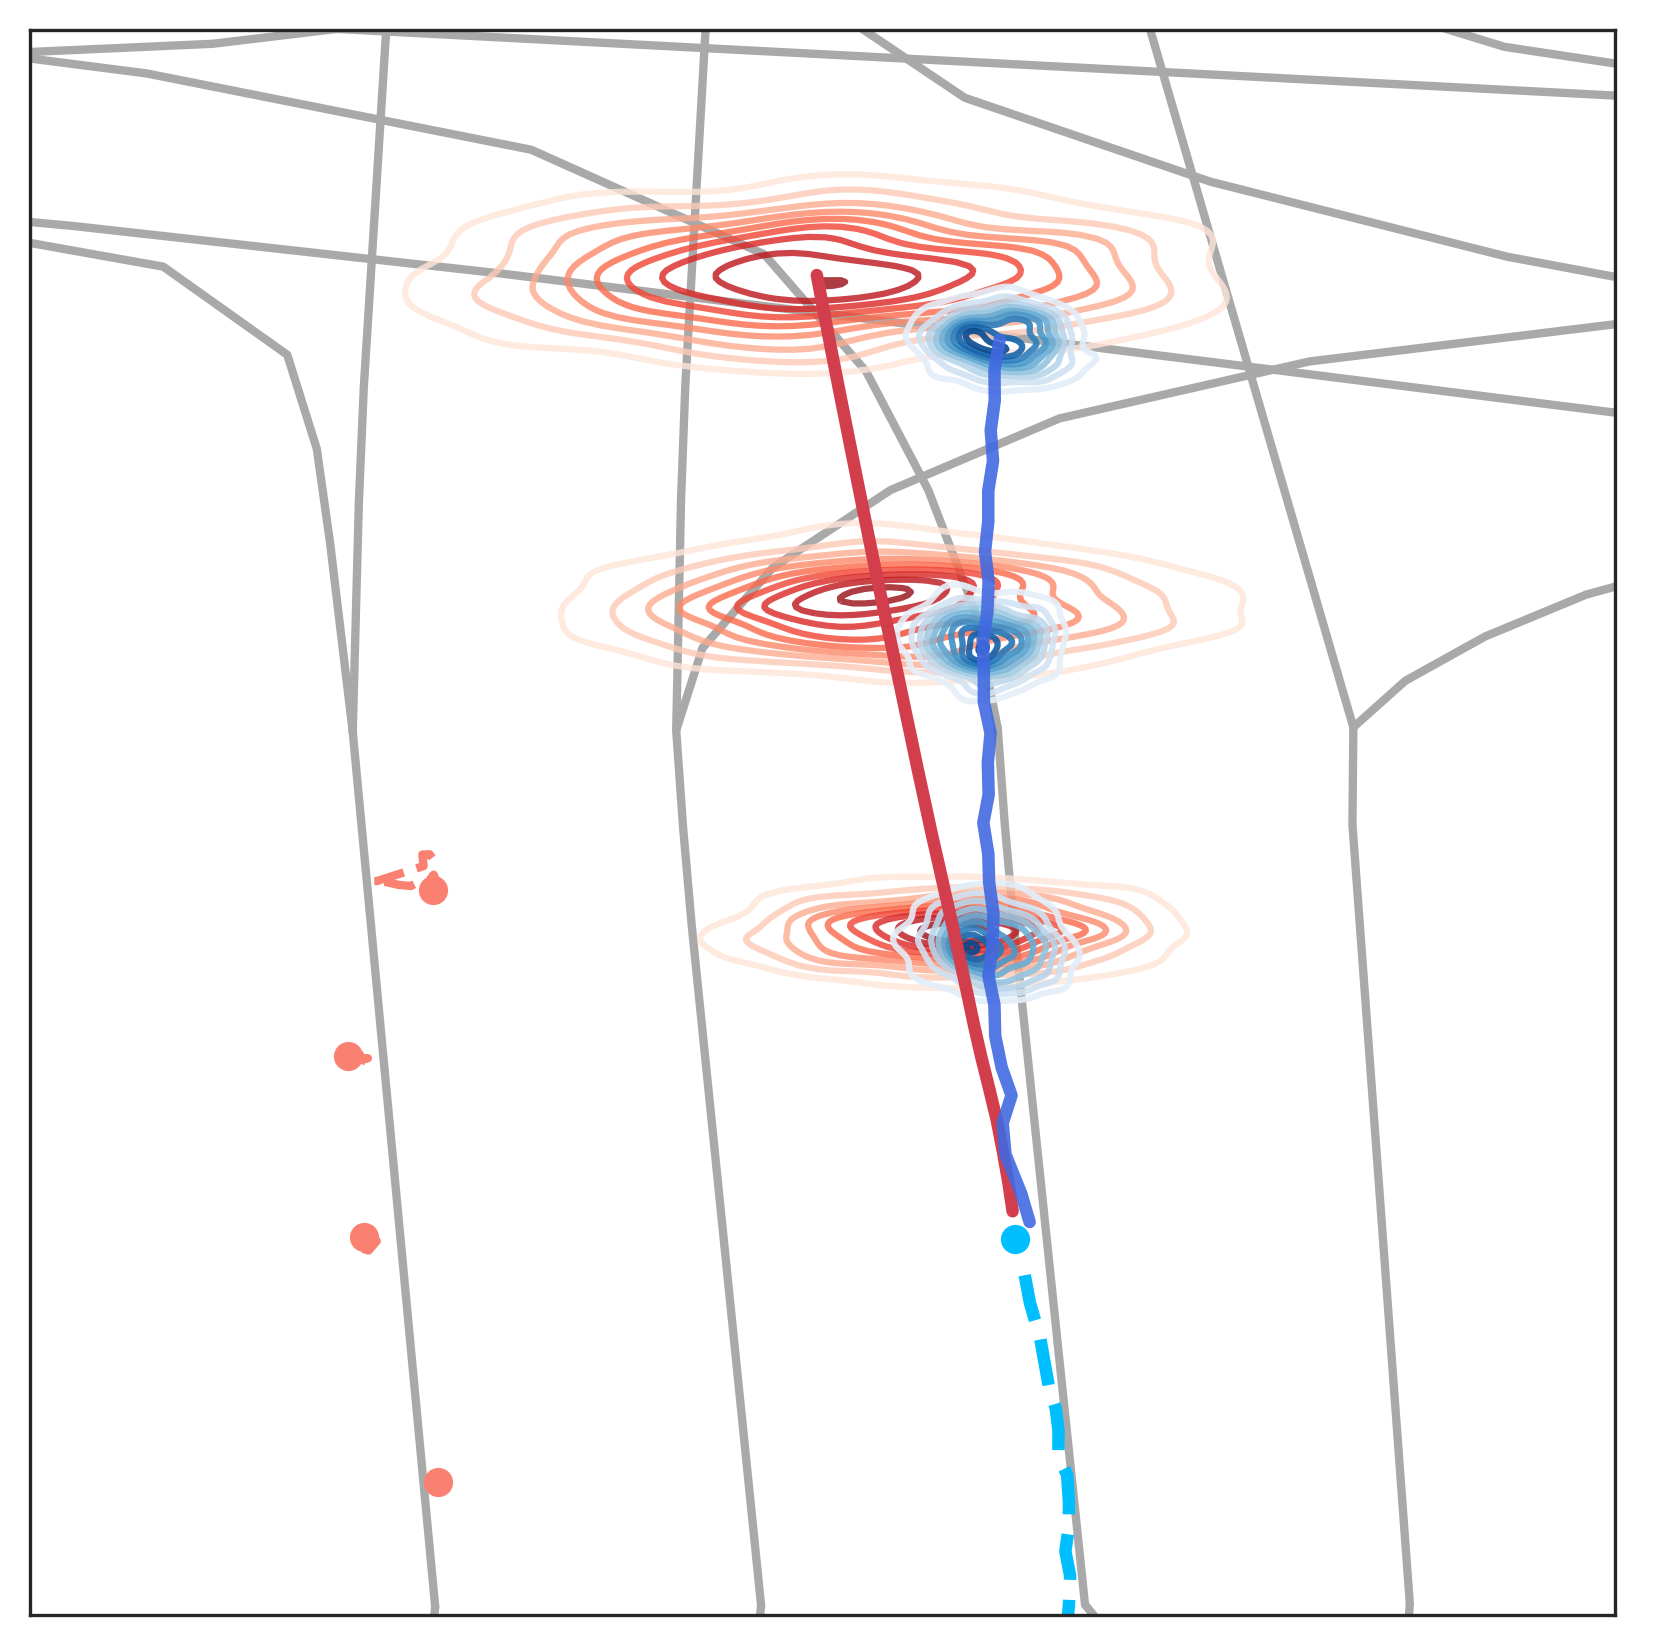
\includegraphics[width=\textwidth]{equivariance/figs/rot1.png}
        \caption{Original scene}
        \label{fig:noneq0}
    \end{subfigure}
    \hspace{2em}
    \begin{subfigure}[b]{0.35\textwidth}
        \centering
        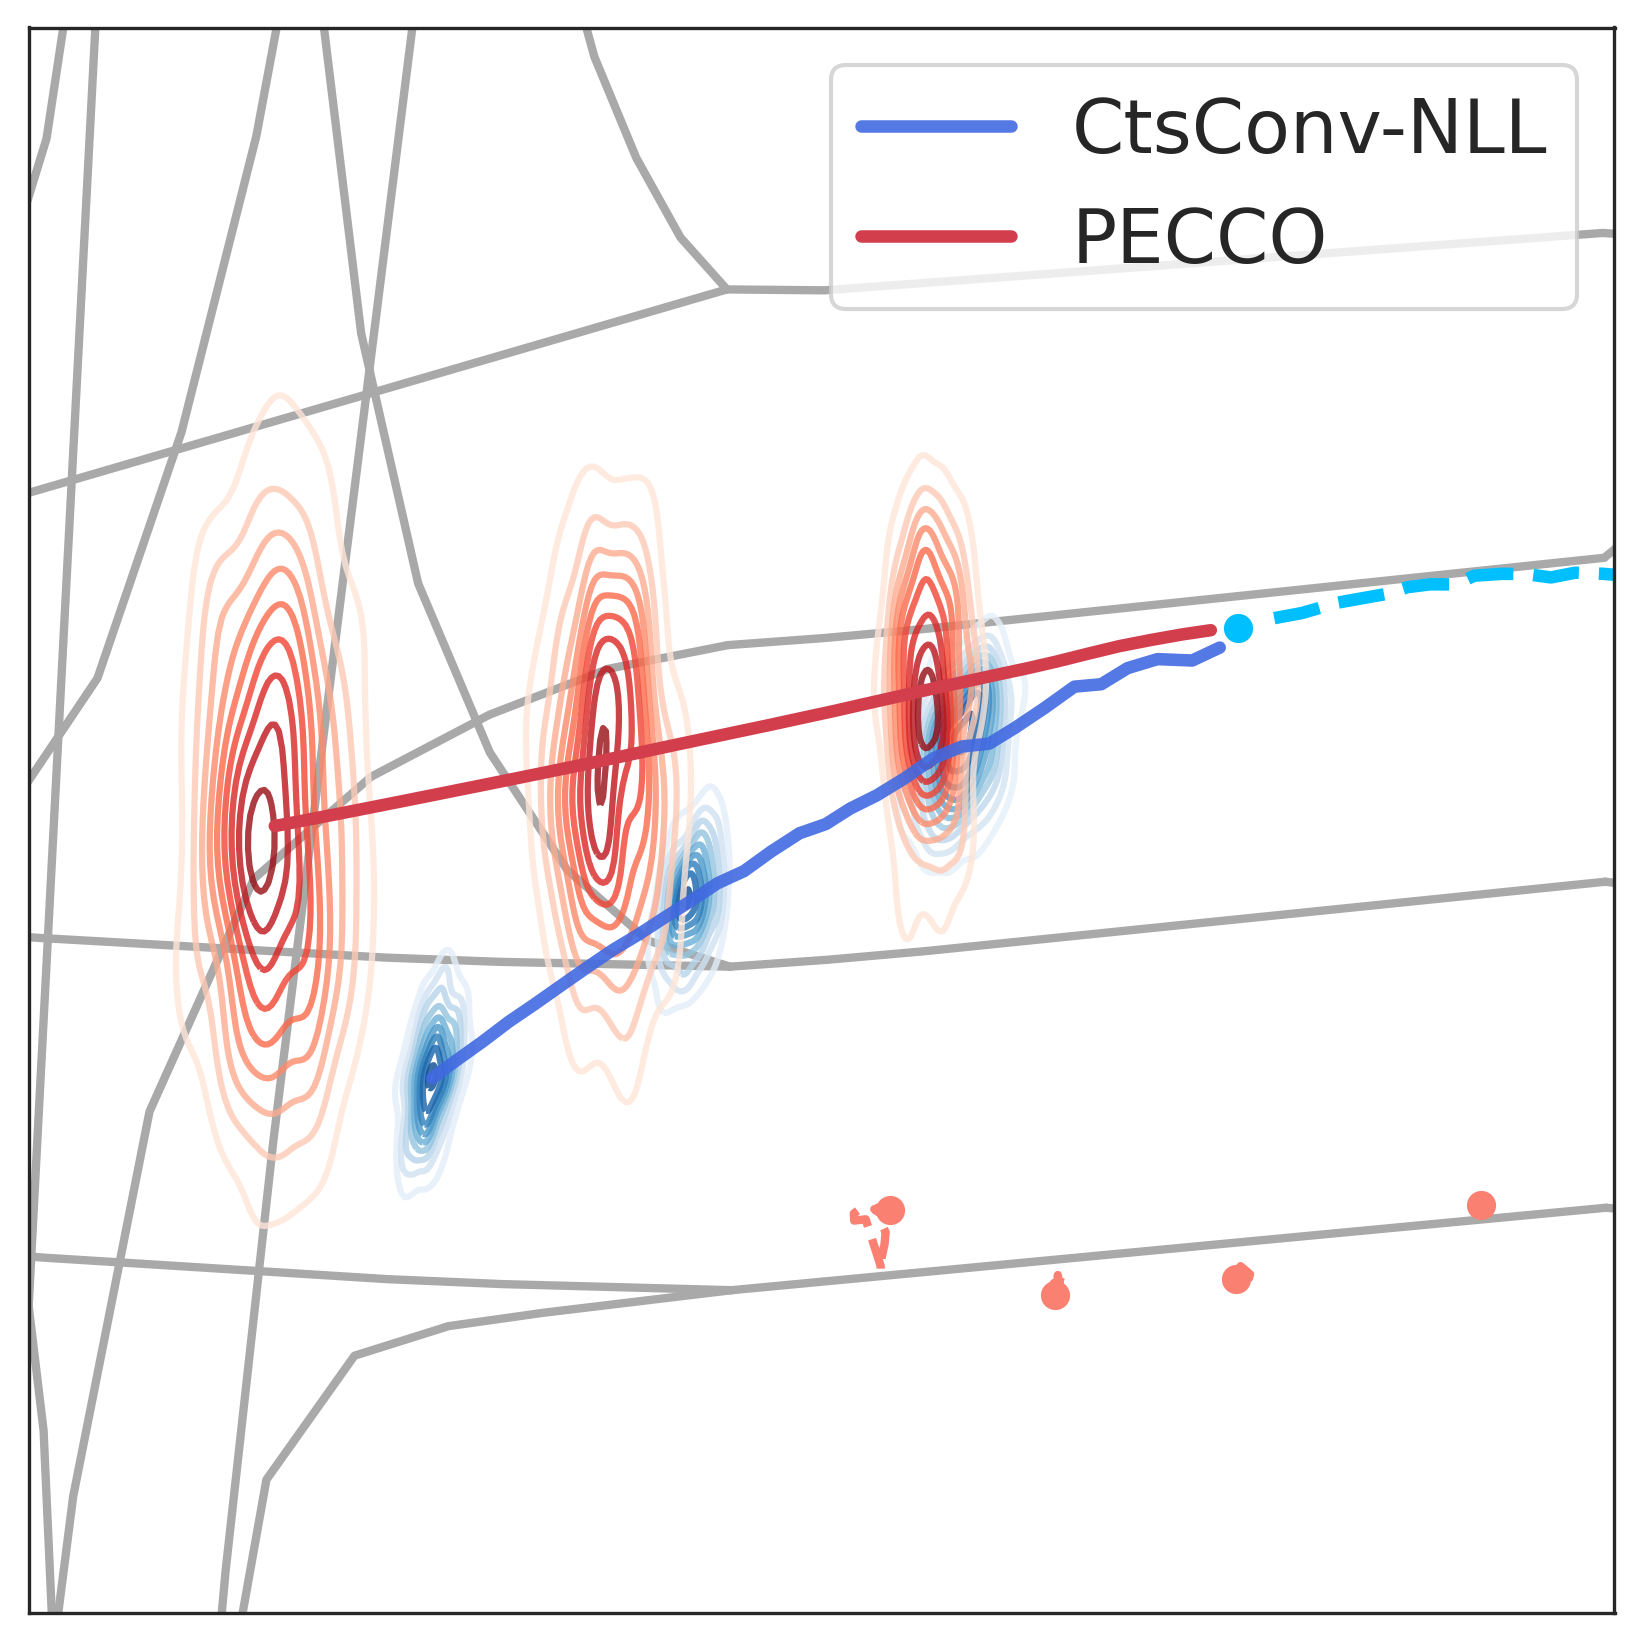
\includegraphics[width=\textwidth]{equivariance/figs/rot2.png}
        \caption{Rotated scene}
        \label{fig:eq0}
    \end{subfigure}
    \caption{Prediction on the same scene rotated by 90 degrees. PECCO is consistent in trajectory and uncertainty prediction, whereas the non-equivariant model (CtsConv) fails.}
    \label{fig:rotpred}
\end{figure}


In this paper, we propose a \textbf{P}robabilistic \textbf{E}quivariant \textbf{C}ontinuous \textbf{CO}nvolutional model (PECCO). PECCO is an equivariant probabilistic trajectory prediction model. Our key insight is to exploit \textit{symmetry} to estimate multidimensional conditional distributions with limited data.  We assume the predicted probability distribution is rotation and translation equivariant. That is, if the input data is transformed, the probability distribution will also be likewise transformed. In Figure \ref{fig:rotpred}, we see the same car approaching an intersection from either the south or east. The scenes are related by a $\pi/2$ rotation.  As the absolute compass direction is not particularly meaningful for local trajectory prediction, the model should thus output the same probability distributions over future trajectories for the car coming from the east as that coming from the north, but rotated by $\pi/2$.  Rotational equivariance not only allows our model to produce physically consistent predictions, the multiplicative nature of equivariance also allows us to model a probability space with a smaller sample size \cite{JMLR:v21:19-322}. For each sample which an equivariant model is trained on, an equivariant model learns as if it were trained on all transformations of that sample by the symmetry group \cite{wang2020incorporating}. 


PECCO also mitigates issues posed by other methods for enforcing equivariance such as data augmentation and normalization. Data augmentation adds rotated versions of data samples to the training dataset such that the model learns rotational equivariance. However, this slows training drastically, requires greater model capacity, and rarely achieves the level of equivariance or accuracy as equivariant neural networks \cite{trajectron++}. Data normalization is a technique that rotates the scene to the agent's reference frame for each data sample, as in \cite{vectornet}.  However, in the multi-agent setting, it is impossible to rotate the scene for multiple agents without a canonical reference frame. PECCO allows the weights to be relative to the local orientation of each agent without the need to rotate the scene repeatedly.   


Our main contributions are two folds: (1) We design an equivariant neural network, PECCO, for probabilistic forecast of multi-agent dynamics, and (2) we demonstrate that by incorporating symmetry, PECCO improves both calibration and sharpness of probabilistic forecasts on a synthetic particle dataset and two real-world benchmark datasets. 



% Effectively, we exploit a symmetry in the conditional probability distribution to factor out orientation, reducing dimensionality, and increasing the number of relevant samples for each prediction.  Intuitively, in order to make predictions for a given agent, our model will be able to generalize from similar samples in the training data regardless of which orientation or position those samples  occur in.     %that could be illustrated by showing say 10 samples in different orientations rotated to the same orientation to show a distribution.


  % Continuous convolution \cite{ummenhofer2019lagrangian} was designed \rw{has been used for} for particle-based fluid simulations. 
 %
%PECCO uses continuous convolution \cite{ctsconv} and enforces rotational equivariance as in \cite{ecco}, achieving more accurate and calibrated probabilistic forecasts. Continuous convolution generalizes discrete convolution and is useful for modeling interactions in many particle systems.

%   This way, our model is able to better estimate the probability for trajectory forecasts.
% Though similar  to graph convolution, like discrete convolution the weights are anisotropic and depend on the relative position of the two particles.   We use rotationally equivariant continuous convolutions as in \cite{ecco} in order to learn model weights which are relative to the local frame of each agent.  Our network is equivariant to rotation, translation, and permutation of particle labels, leading to improved coverage and consistency of predicted uncertainties. %generalization and consistency


% We evaluate our model on two datasets: Argoverse autonomous vehicle dataset \cite{argoverse} and TrajNet++ pedestrian trajectory forecasting challenge \cite{pedestriandata}. We demonstrate that in addition to enabling more accurate trajectory prediction, equivariance also improves the quality of uncertainty estimates in the context of trajectory prediction.


%\item We introduce a new metric, mean regional score (MRS), to evaluate the quality of probabilistic forecasts.
   

%In this work we present a multi-agent motion prediction model that are both equivariant and probablstic. 


% Trajectory prediction is one of the core tasks in AI,  from the movement of basketball players to fluid particles to car traffic \cite{sanchez2020learning, gao2020vectornet, shah2016applying}. 
% A common abstraction underlying these tasks is the movement of many interacting agents, analogous to  a many-particle system. Therefore,  understanding  the states of these particles, their  dynamics,  and hidden interactions is critical to accurate and robust trajectory forecasting.

% \begin{wrapfigure}{r}{0.5\textwidth}
% \vspace{-0.4cm}
%   \begin{center}
%     \includegraphics[width=0.5\textwidth,trim=40 30 40 20, clip]{figs/fig1.png}
%   \caption{Car trajectories in two scenes.  Though the entire scenes are not related by a rotation, the circled areas are.  \ours{} exploits this symmetry to improve generalization and sample efficiency.}
%   \end{center}
%   \vspace{-3mm}
%   \label{fig:twoscenes}
% \end{wrapfigure}

%  Even for purely physical systems such as in particle physics, the complex interactions among a large number of particles makes this a difficult problem.  For vehicle or pedestrian trajectories, this challenge is further compounded with latent factors such as human psychology.  Given these difficulties, current approaches require large amounts of training data and many model parameters. State-of-the-art methods in this domain such as %\cite{liang2020learning} and
%  \cite{gao2020vectornet}  
%  are based on graph neural networks. They do not exploit the physical properties of system and often make predictions which are not self-consistent or physically meaningful. Furthermore, they predict a single agent trajectory at a time instead of multiple agents simultaneously. %  \ry{need better argument}  
% % Furthermore, these methods adopt the perspective of a single agent in the scene, making it hard to produce consistent trajectories for all agents simultaneously. % 

% % \ry{this fig is taking too much space, make it compact}
% % \begin{figure}[b!]
% %     \centering
% %     \includegraphics[width=10cm,trim=0 0 0 20, clip]{figs/fig1.png}
% %     \caption{Car trajectories in two scenes.  Though the entire scenes are not related by a rotation, the circled areas.  ECCO exploits this symmetry to improve generalization and sample efficiency.}
% %     \label{fig:twoscenes}
% % \end{figure}




% Our model is built upon a key insight of  many-particle systems pertaining to intricate internal symmetry. Consider a model which predicts the trajectory of cars on a road.  To be successful, such a model must understand the physical behavior of vehicles together with  human psychology. It should distinguish left from right turns, and give consistent outputs for intersections rotated with different orientation. As shown in \autoref{fig:twoscenes}, a driver’s velocity rotates with the entire scene, whereas vehicle interactions are invariant to such a rotation. Likewise, psychological factors such as reaction speed or attention may be considered vectors with prescribed transformation properties. Data augmentation is a common practice to deal with rotational invariance, but it cannot guarantee invariance and requires longer training. Since rotation is a continuous group, augmentation requires sampling from infinitely many possible angles.

% %  In our model, this is achieved by considering all hidden layers to be vectors with the prescribed action of a symmetry group.



% In this paper, we propose an equivariant continuous convolutional model, \ours{}, for trajectory forecasting. % Continuous convolution \cite{ummenhofer2019lagrangian} was designed \rw{has been used for} for particle-based fluid simulations. 
%  %
%  Continuous convolution generalizes discrete convolution and is adapted to data in  many-particle systems with complex local interactions. \citet{ummenhofer2019lagrangian} designed a model using continuous convolutions for particle-based fluid simulations.
% %
% Meanwhile, equivariance to group symmetries has proven to be a powerful tool to integrate physical intuition  in physical science applications  \cite{wang2020incorporating, brown2019equivariant, kanwar2020equivariant}.  Here, we test the hypothesis that an equivariant model can also capture internal symmetry in non-physical human behavior. Our model utilizes a novel weight sharing scheme, torus kernels, and is rotationally equivariant.

% %  We perform an ablative study to validate the importance of different aspects of our model.
  
% We evaluate our model on two real-world trajectory datasets: Argoverse autonomous vehicle dataset \cite{chang2019argoverse}  and TrajNet++ pedestrian trajectory forecasting challenge \cite{kothari2020human}.       We demonstrate on par or better prediction accuracy to baseline models and data augmentation with fewer parameters, better sample efficiency, and stronger generalization properties.  Lastly, we demonstrate theoretically and experimentally that our polar coordinate-indexed filters have lower equivariance discretization error due to being better adapted to the symmetry group.  

% Our main contributions are as follows:
% \begin{itemize}
%     \item We propose \textbf{E}quivariant \textbf{C}ontinous \textbf{CO}nvolution (\ours{}), a rotationally equivariant deep neural network that can capture internal symmetry in trajectories. 
%     \item We  design \ours{} using a novel weight sharing scheme based on orbit decomposition and polar coordinate-indexed filters. We implement equivariance for both the standard and regular representation $L^2(\mathrm{SO}(2))$.
%     \item On benchmark Argoverse and TrajNet++ datasets, \ours{} demonstrates  comparable accuracy  while enjoying better generalization, fewer parameters, and better sample complexity.
%     % \item We demonstrate theoretically and experimentally that despite discretization our polar coordinate-indexed filters have very low equivariance error. \ry{not clear the significance}  
% \end{itemize}

\section{Related Work}
\paragraph{Trajectory Prediction.} 
% to potential-based methods such as Inverse Reinforcement Learning \cite{irl} and Recurrent Neural Networks (RNN) powered ones \cite{rnn1, sociallstm}.
%
Multi-agent trajectory forecasting has been extensively studied, 
approaches ranged from Kalman filters \cite{kalman1960} to non-linear Gaussian Process Regression models \cite{gaussianprocess}. However, these methods either rely on strong assumptions of the dynamics, or do not explicitly model multi-agent interactions. We refer readers to \cite{trajpredsurvey} for a comprehensive survey of such methods. 
%
Advancements in deep learning have allowed  flexible modeling of trajectory dynamics \cite{sociallstm, ctsconv, convsocialpooling, sophie, laneGCN, ecco, vectornet, simplex}, but they focus mainly on point estimation without uncertainty. 


% Various approaches explored leveraging the structure of physical data to encode neighboring vehicle interaction - from  grid representations \cite{convsocialpooling}, graph neural networks \cite{lanegraph, vectornet}, to simplicial complexes \cite{simplex}. 

% The former represent the distribution in the form of a 2-dimensional Gaussian Mixture Model (GMM) where the latter \ry{add details}. 

Recent methods have shifted to predicting distributions of  future trajectories, capturing uncertainty in dynamics. There are two main categories for probabilistic forecasting: (1) \textit{explicitly} via exact likelihood \cite{mfp, multipath,densetnt} and variational inference \cite{CVAE, trajectron++, desire}, or (2) \textit{implicitly} with Generative Adversarial Networks (GANs) \cite{socialgan,liu2019naomi}. Our work falls into the first category where we model the distributions parametrically. Parametric models allow us to evaluate the likelihood of future trajectories, which are useful for downstream planning tasks \cite{multipath, schwarting2018planning}.

%\cite{propogating} studies how perceptual uncertainty can be incorporated into trajectory prediction. 
Despite the development in probabilistic modeling, there is no standard metric for quantifying uncertainty of the prediction. Negative log likelihood often overfits the distribution \cite{guo2017calibration}, and best-of-n-sample results do not evaluate the full distribution \cite{rethinking}. We argue that probabilistic forecasts should accurately reflect the uncertainty in the model predictions. We propose using proper scoring rules such as Energy Score or mean interval score \cite{properscoring} for evaluating probabilistic forecasts. 
% For example, in the scenario of an intersection where there are many possible futures, nll-based methods often collapses to the most likely mode and underestimate the possible range of trajectories, whereas an interval-based method would \ry{what?}. %\sofi{example for MIS}
%Furthermore, by leveraging the internal symmetries of trajectories, our model produces more accurate and calibrated probabilistic forecasts.


%cite papers form ICLR ICML NeurIPS CVPR likely from community - reduce intelligent transport 

\paragraph{Equivariant Deep Learning.}
Geometric deep learning that leverages invariance and symmetries has found wide applications in areas ranging from image recognition \cite{bao2019equivariant, worrall2017harmonic, weiler2019e2cnn} to reinforcement learning \cite{equimdp}. Equivariant neural networks are studied for modeling dynamics as well - \cite{fuchs2020se} use $\mathrm{SE}(3)$-equivariant transformers to predict trajectories for a small number of particles as a regression task, and \cite{ecco} proposed a $\mathrm{S0}(2)$ equivariant continuous convolution for traffic trajectory prediction. All the methods mentioned above are deterministic. \cite{kohler2020equivariant} and \cite{ennormalizingflows} studies equivariant normalizing flows for modeling symmetric densities, however their domains focus on generative modeling and therefore differ from our work significantly. To our knowledge, no previous work has studied equivariant neural networks for probabilistic dynamics forecasting. 

\paragraph{Uncertainty Quantification (UQ).}
Uncertainty quantification is critical for risk assessment in safety-critical domains. Properly quantified uncertainties can be used to create probabilistic constraints and generate more robust planning and control strategies \cite{ostafew2016learning, bujarbaruah2019adaptive}. With the increasing use of deep learning in forecasting tasks, many works have UQ for neural networks \cite{saftyassurance, wu2021quantifying, guo2017calibration}. \cite{2021conformal} proposes a conformal prediction algorithm for 1D RNN forecasters with a prediction region with coverage guarantees. However, these works focus only on classification or 1-dimensional forecasts. \cite{salinas2019high, salinas2020deepar} use autoregressive RNNs for probabilistic forecasting of multiple time series, however, their method cannot explicitly model spatial relations. We present a model design for multi-agent dynamics and produce probabilistic distributions with better calibration.
% In our experiments, we show that the uncertainty distributions produced by deep generative models for trajectory forecasting are often not calibrated. Hence, better UQ methods are needed. In this work, we expand metrics from quantile and conformal prediction to the multivariate setting, and introduce a method to evaluate forecasted uncertainties.

\section{Background}
We give a short background on  symmetry and equivariance and their probabilistic extension.
%
\paragraph{Symmetry and Equivariance.}\label{subsec:symmetry}
A \emph{symmetry group} $G$  is a set together with a composition operation $\circ \colon G \times G \to G$ which is associative and has an identity and inverses. The group $G$ can transform a vector space $V$ by specifying a \emph{representation} which is a mapping $\rho \colon G \to \mathrm{GL}_n(V)$ sending each element of the group $G$ to an invertible $n \times n$ matrix such that $\rho(g_1 \circ g_2) = \rho(g_1) \rho(g_2)$.  

Given a function $f \colon X \to Y$ such that $G$ has representations $\rho_X$ and $\rho_Y$ acting on $X$ and $Y$ respectively, we say $f$ is $G$-\emph{equivariant} if for all $x \in X$ and $g \in G$, we have $\rho_Y(g)f(x) = f(\rho_X(g) x )$.  That is, a transformation of the input of $x$ induces a corresponding transformation of the output.  \emph{Invariance} for the function $f$ is a special case in which $\rho_Y(g)y = y$. 

% \paragraph{\texorpdfstring{$\mathbf{SO(2)}$}{SO(2)} Rotational Symmetry.}

% In this paper, we consider  equivariance to 2D planar rotations, $\SOtwo = \{ \Rot_\theta : 0 \leq \theta < 2 \pi \}$
% which has composition $\Rot_{\theta_1} \circ \Rot_{\theta_2} = \Rot_{(\theta_1 + \theta_2) \mathrm{mod} 2 \pi}$.  As a Lie group, $\SOtwo$ also has an underlying topological structure given by the manifold $S^1 \cong \lbrace \rvx \in \mathbb{R}^2 : \| \rvx \|=1 \rbrace$.  
% Here, we consider two specific representations of $\SOtwo$. 
% The \textit{standard representation} $\rho_1$ on $\mathbb{R}^2$ is by $2 \times 2$ rotation matrices. The \textit{regular representation} $\rhoreg$ on $L^2(\SOtwo) = \lbrace \varphi: \SOtwo \to \mathbb{R} : |\varphi|^2 \text{ is integrable} \rbrace$ is  $\rhoreg(\Rot_\phi)(\varphi) = \varphi \circ \Rot_{-\phi}$. Here $L^2$
% is a Hilbert space.

\paragraph{\texorpdfstring{$\mathbf{SO(2)}$}{SO(2)} Equivariant Continuous Convolution.}
% - ECOO impliments SO(2)-equiv cts conv.
% - add eqn for cts conv
Continuous convolution \cite{ummenhofer2019lagrangian} generalizes discrete convolution. The feature vector $\mathbf{f}^{(i)} \in \mathbb{R}^{c_\mathrm{in}}$ of particle $i$ forms a vector field $\mathbf{f}$, and the kernel of the convolution $K: \mathbb{R}^2 \mapsto \mathbb{R}^{c_\mathrm{out}\times c_\mathrm{in}}$ forms a matrix field: for each point $\mathbf{x} \in \mathbb{R}^2$, $K(\mathbf{x})$ is a $c_\mathrm{out}\times c_\mathrm{in}$ matrix. The continuous convolution is then defined by 
\[
 \mathbf{g}^{(i)} = \sum_j a(\|\mathbf{x}^{(j)} - \mathbf{x}^{(i)}\|) K(\mathbf{x}^{(j)} - \mathbf{x}^{(i)}) \cdot \mathbf{f}^{(j)}.
\]
By \cite{weiler2019e2cnn}, this is $\SOtwo$-equivariant if 
$
K(gv) = \rho_\mathrm{out}(g) K(v) \rho_\mathrm{in}(g^{-1})$.

ECCO \cite{ecco} defines the convolution kernel $K$ in polar coordinates $K(\theta, r)$. Let $\mathbb{R}^{c_\mathrm{in}}$ and $\mathbb{R}^{c_\mathrm{out}}$ be $\SOtwo$-representations $\rho_\mathrm{in}$ and $\rho_\mathrm{out}$ respectively, then the convolution kernel satisfies the equivariance condition as follows, making the continuous convolution $\SOtwo$-equivariant.
\[
 K(\theta + \phi, r) = \rho_\mathrm{out}(\mathrm{Rot}_\theta) K(\phi,r)\rho_\mathrm{in}(\mathrm{Rot}_\theta^{-1})
\]


%We say a function $f$ is group equivariant iff it satisfies 
%\[\rho(g) f(x) = f(\rho'g(x))  \] where $\rho(\cdot)$ and $\rho'(\cdot)$ are the representation of the group $g \in G$.

% If $X$ is a random variable, we need to define an estimator $\delta$ such that $\delta$ is G-equivariant.
% \[  \rho(g) \delta(x) = \delta (\rho'(g(x)), \quad \forall x \sim p(x) \]
% For example, $\delta$ can be the maximum likelihood estimator of a distribution. That is 
% \begin{equation}
%     \delta(X) = \max_{\theta} \sum_{i=1}^N \log p(\V{x}^{(i)}), \quad  \T{P}(X) = \{ p_{\theta}(\V{x}): \V{x}\in \Omega \}
%     \label{eqn:mle}
% \end{equation}
% where $\V{x} = (x_1, \cdots, x_T)$
% For a sequence of random variables, such as uncorrelated  standard normal distribution, it is rotational invariant. 

% \sofi{the definition of equivariance in a probabilistic setting (check frank noe papers for presentation and citations)}

% \ry{generalize De Finetti's theorem to other groups}

% Group action 
% \sofi{ROT function on a distribution (map from R2 to [0,1] satisfying integration to 1). Assume f is a gaussian PDF, show that it naturally extends. make whole story}


\paragraph{Calibration and Sharpness of Probabilistic Prediction.} 
It is desirable for a probabilistic prediction to be both \textit{calibrated} and \textit{sharp}. A model is \textit{calibrated} when the predicted probability correspond to the true probability of an event. In forecasting, calibration is often measured with \textit{coverage}, the probability of ground truth ${Y}$ falls into prediction region of confidence $\Hat{C}^{1-\alpha}$, $1-\alpha \in [0,1]$. 
\begin{align}
    P(Y \in \Hat{C}^{1-\alpha}) \geq 1- \alpha
    \label{eq:coverage}
\end{align}
%The forecast is \textit{valid} if it satisfies \autoref{eq:coverage}, and calibrated in case of equality.
Note that one can always obtain a calibrated prediction region by setting $\Hat{C}^{1-\alpha}$ to be the entire $Y$ space. We introduce the concept of  \textit{Sharpness}, which refers to the size of the prediction region $|\Hat{C}^{1-\alpha}|$. The balance between calibration and sharpness can be measured by a class of metrics called proper scoring rules \cite{properscoring}.
\vskip -0.1 in

%\section{Score Function for Probabilistic Forecast} 
%\input{secs/problem}
\section{PECCO}

\begin{figure}[ht!]
  \centering
  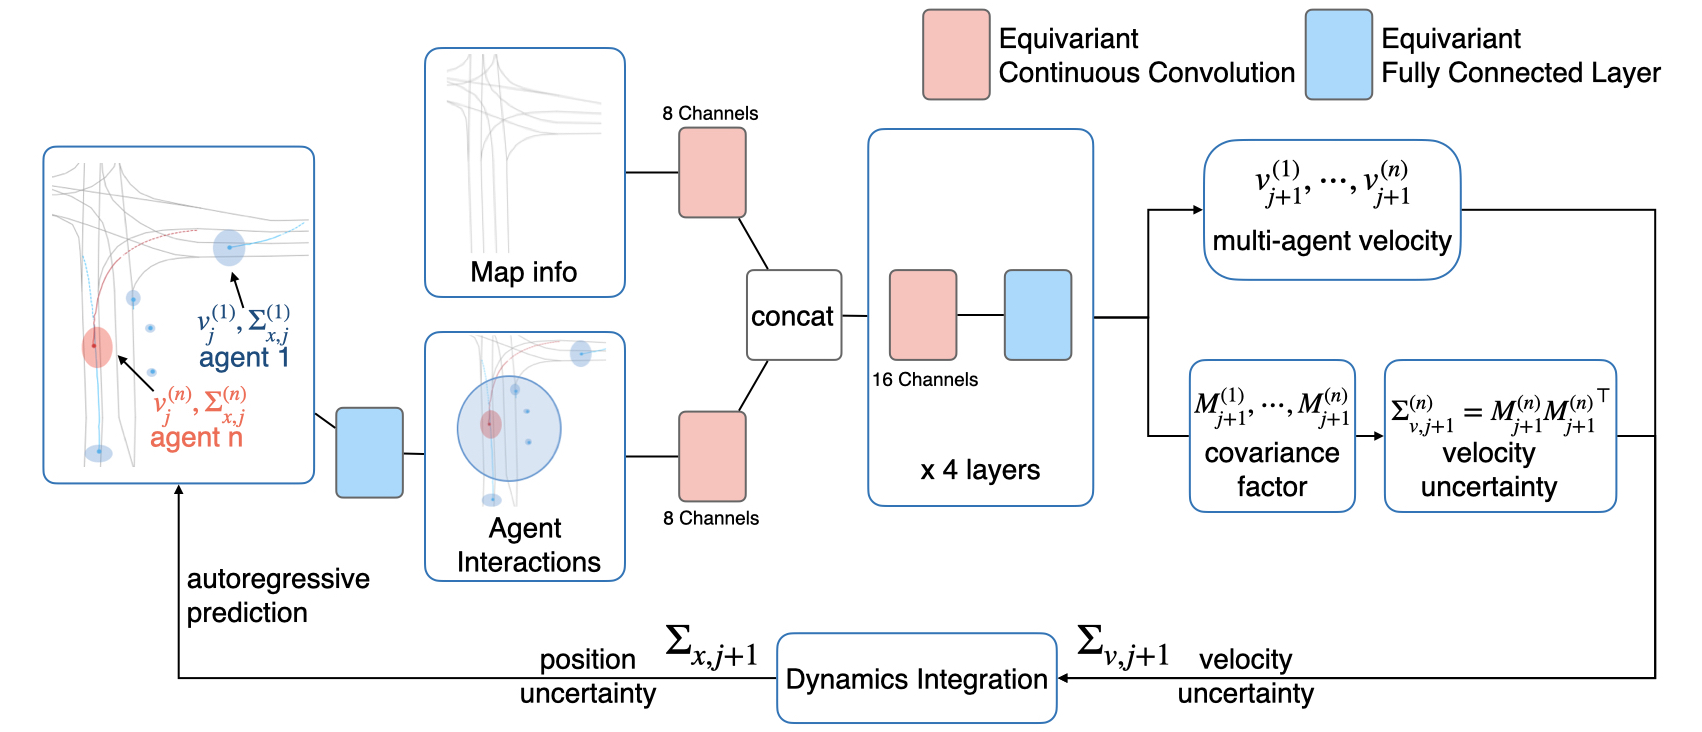
\includegraphics[width=1\linewidth]{equivariance/figs/model2.jpeg}
  %model.pdf
  \caption{Overview of PECCO's model architecture. Agent trajectories consisting of velocities and position uncertainties are encoded along with map information by equivariant continuous convolution and fully connected layers. The model outputs $v_{j+1}$ and $\Sigma_{v,j+1}$ for all agents, which we use to calculate position uncertainty $\Sigma_{x,j+1}$ via dynamics. The model takes in the forecast and predicts autoregressively.} 
  \label{fig:model}
\end{figure}

\subsection{Problem Setup}
 Given  past trajectories of $n$ agents over $t$ time steps $\{x_{j}^{(1)}, x_{j}^{(2)}, \cdots, x_{j}^{(n)} \}_{j=1}^t $, where  ${x}^{(i)}_{j} \in \mathbb{R}^2$ , and the environmental context information $\mathbf{e}$ including marker positions of map lane boundaries, we model the probability distribution of agents' positions over  $k$ future time steps  as $p_\theta( {x}_{t+1:t+k} | {x}_{1:t}, \mathbf{e})$, with ${x}_j = ({x}^{(1)}_{j},\cdots, {x}^{(n)}_{j})$ being the positions of all agents at time step $j$. We introduce  PECCO, a deep learning model that leverages rotational equivariance to produce probabilistic forecasts.


The high-level architecture of our model is illustrated in Figure \ref{fig:model}. PECCO takes as input the positions of all agents ${x}_{1:t}$ in the past, and the covariance matrix $\Sigma_{x,j}$ at time $j$. It outputs the probability distribution of each agents' velocity as a 2-D Gaussian $\T{N}(\mu_{v,j+1}^{(i)}$, $\Sigma_{v,j+1}^{(i)})$ for the next time step. The velocity distribution is then integrated into a position distribution $\mathcal{N}$($\mu_{x, j+1}^{(i)}$, $\Sigma_{x, j+1}^{(i)}$) through dynamics integration. PECCO predicts the future $k$ timesteps autoregressively. The output distributions are guaranteed to be rotational equivariant by our model implementation.

\subsection{Probabilistic Symmetry through Equivariant Neural Networks} 

Rotational equivariance effectively reduces the dimension of the data space by placing different samples in the same equivalence class. This improves data coverage for better probabilistic modeling. 

Intuitively, real-world trajectory dynamics has intrinsic symmetry. That is, if past trajectories and environmental data such as the map is rotated, then the probability of a rotated future trajectory will be equally likely. We can model the probability density function $p_\theta$ as an invariant function of its inputs as in \autoref{eqn:invariant_prob}. Here, each past and future position $x^{(i)}_j \in \mathbb{R}^2$ is transformed according the standard representation $\rho_1$.  
\begin{equation} \label{eqn:invariant_prob}   
    p_\theta( {x}_{t+1:t+k} | {x}_{1:t}, \mathbf{e}) = p_\theta( g{x}_{t+1:t+k} | g{x}_{1:t}, g\mathbf{e}) \quad \forall g\in \SOtwo
\end{equation}


%\rw{explicitly refer to factorization over agents and timesteps?}

In order to implement \autoref{eqn:invariant_prob}, we 
assume future positions  follow a multivariate normal distribution ${x}^{(i)}_{j} \sim N(\mu^{(i)}_{x,j},\Sigma^{(i)}_{x,j})$. This is a common assumption in trajectory forecasting literature \cite{trajpredsurvey} and provides a convenient parametric form for optimization and reasoning. In the following expositions we omit the underscore $x$ for simplicity.

We aim to construct an equivariant neural network $f_\theta$ that outputs the parameters $\mu^{(i)}_{j}$ and $\Sigma^{(i)}_{j}$ autoregressively, taking as input probability distributions over the positions of all agents in the past $k$ time steps
\[
\mu_{j+1},\Sigma_{j+1} = f_\theta(\mu_{j-t+1:j}, \Sigma_{j-t+1:j}, \mathbf{e}). 
\]
where $\mu_{j} = (\mu_{j}^{(1)},\ldots,\mu_{j}^{(n)})$ and $\Sigma_j = (\Sigma_{j}^{(1)},\ldots,\Sigma_{j}^{(n)})$ and $\mathbf{e}$ denotes environmental information.  

In this case, the equivariance of $f_\theta$ leads to the desired invariance of $p_\theta$. This may be seen as a partial evaluation or currying of the conditional probability density function which has the effect of transforming invariance to equivariance. The following proposition relates equivariant networks with probabilistic symmetry. See Appendix \ref{app:equiv_dist} for a proof.
\begin{proposition}[One step equivariance implies $n$-step equivariance] \label{prop:equivtoinvar}
If the one-step probabilistic forecasting model $f_\theta$ is $G$-equivariant, then the probability distribution $p_\theta( x_{t+1:t+k} | x_{1:t}, \mathbf{e})$ is invariant as in \autoref{eqn:invariant_prob}.
\end{proposition}

%\paragraph{Equivariant Conditional Normal Distributions.} 
In order to enforce $\SOtwo$-equivariance for $f_\theta$, the following proposition describes how the mean and covariance matrix for a 2-D  Gaussian  transforms under a rotation of $\mathbb{R}^2$. 

\begin{proposition}[SO(2) equivariance of multivariate Gaussian]  \label{prop:equivnormal}
Given multivariate normal distribution $\mathcal{N}(\mu,\Sigma)$ over $\mathbb{R}^2$ with probability density function $p_{\mu, \Sigma}$ and $g\in \SOtwo$, then $\mathcal{N}(g\mu, g\Sigma g^T)$ is also a multivariate normal distribution and $p_{g\mu, g\Sigma g^T} (v) = p_{\mu, \Sigma} (g^{-1}v)$ for all $v \in \mathbb{R}^2$.
\end{proposition}  

To ensure the covariance matrix of $f_\theta$ is positive-definite and symmetric, i.e. $\Sigma \in \mathrm{PosDefSym}_2(\mathbb{R})$, we make use of the following fact: 

\begin{proposition}[Equivariant maps constructing positive-definite symmetric matrices] \label{prop:pds}
The map
\begin{align}
    \varphi \colon \mathrm{GL}_2(\mathbb{R}) \to \mathrm{PosDefSym}_2(\mathbb{R}) , \quad 
    M \mapsto M M^T \label{eq:phi}
\end{align}
is surjective and equivariant. That is, for $g \in \SOtwo$ we have
\begin{align}
    \varphi(gM) &= g \varphi(M) g^{T} \label{eq:act_on_gl2}. 
\end{align}
Moreover, $\varphi$ admits a one-sided inverse which is also equivariant,
\begin{align}
        \psi \colon \mathrm{PosDefSym}_2(\mathbb{R}) \to \mathrm{GL}_2(\mathbb{R}), \quad    
        \Sigma \mapsto Q \Lambda^{\frac{1}{2}}
\end{align}
where $Q\Lambda Q^T$ is the eigendecomposition of $\Sigma$ and $Q$ is orthogonal. Together, $\varphi (\psi(\Sigma)) = \Sigma$.
\end{proposition}

As a consequence of Proposition \ref{prop:equivnormal} and Proposition \ref{prop:pds}, we can ensure that the predicted distribution transforms correctly under equivariance by (1) predicting an intermediate matrix $M$ for covariance, and (2) constraining $\tilde{f}_\theta$ to be equivariant with respect to the action in \autoref{eq:act_on_gl2}.
\begin{equation} \label{eq:ftheta}
\begin{aligned}    
    \mu_{j+1},M_{j+1} = \tilde{f}_\theta(\mu_{j-k:j}, M_{j-k:j}, \mathbf{e}), \;
    \Sigma_{j+1} = M_{j+1}M_{j+1}^T
\end{aligned}
\end{equation}
In this case, $\SOtwo$ acts by transforming the the columns of $M$ independently as vectors in $\mathbb{R}^2$.  Thus the data $(\mu_j^{(i)},\Sigma_j^{(i)})$ for each agent and time step is comprised of 3 copies of the standard representation $\rho_1$ as defined in Section \ref{subsec:symmetry}.  Given this $\SOtwo$ action, we can enforce $\SOtwo$-equivariance in the neural network $\tilde{f}_\theta$. Implementation details of  of the equivariant layers are provided in Appendix \ref{app:matrix}.


% \begin{proposition}
% If $f_{\theta}$ satisfies then $f_{\theta}$ is equivariant
% \end{proposition}

% [REFERNCE STUFF FROM APPENDIX HERE.  NO PROOFS JUST STATEMENT AND SHORT DESCRIPTION]


%\subsection{Kernel and Weight Sharing Scheme} 

\subsection{Dynamics Integration (dyna)} 
\label{sec:dyn_inte}
Instead of predicting the position directly, PECCO outputs a Gaussian distribution over \emph{velocity} as $\mathcal{N}(\mu_{v,j}, \Sigma_{v,j})$. More specifically, it predicts $(\mu_{v,j}, M_{v,j})$ at each time step and the covariance matrix $\Sigma_{v,j}$ is calculated as in Proposition \ref{prop:pds}. However, we want to obtain the  uncertainty over \textit{position} as $\Sigma_{x,j}$ and perform autoregressive forecasting. We leverage dynamics integration to propagate the uncertainty from velocity to position.


Assuming that all agents in the system can be approximated as linear discrete time dynamics ${x}_{j+1} = {x}_j + \Delta t \cdot  {v}_j $, we can obtain the uncertainty of predicted position $\Sigma_{x, j+1}$ by %  =  \Sigma_{p, t} + \Delta t \cdot \Sigma_{v,t+1}\cdot\Delta t 
\[ 
\Sigma_{x, j+1}
            = \Sigma_{x, j} + (\Delta t)^2 \, \Sigma_{v, j} + 2 \Delta t \cdot \text{cov}(x_j, v_j).
\]
%
We assume that the cross covariance matrix $\mathrm{cov}(x_j, v_j) $ is zero for simplicity 
following previous works \cite{trajectron++}. During training, gradients are calculated after entire trajectory is predicted autoregressively. A consequence of the additive uncertainty setup is that it enforces the uncertainty 
to grow monotonically over time, creating a ``cone of uncertainty".


\section{Experiments}

We show that our model produces accurate and more calibrated probabilistic forecast compared to baseline models on one synthetic and two real world trajectory prediction datasets: interacting particles, autonomous vehicle, and pedestrian movement. 
\subsection{Baselines}
%We compare our model PECCO against the following baselines:
\begin{itemize}
\itemsep0em 
   \item \texttt{LSTM-NLL} (variation of \cite{sociallstm}): An encoder-decoder LSTM model that predicts the mean and variance of a Gaussian distribution, optimizing likelihood of data. We also train a version with random rotation data augmentation \texttt{LSTM-aug}.
    \item \texttt{CtsConv} \cite{ummenhofer2019lagrangian}: Continuous convolution over point cloud data for trajectory prediction, a non-equivariant counterpart of PECCO. \texttt{CtsConv-aug} is trained with a data augmentation step where we randomly rotate the scenes. 
    %\item \texttt{ECCO} \cite{ecco}: State-of-the-art equivariant model for deterministic trajectory prediction. 
     \item \texttt{Multiple Futures Prediction (MFP)} \cite{mfp}: A encoder-decoder model for multimodal probabilistic trajectory forecasts.
     \item \texttt{Trajectron++} \cite{trajectron++}: State-of-the-art probabilistic trajectory prediction model with graph representation of agent interactions and conditional VAE architecture.
\end{itemize}
% For the deterministic models (\texttt{LSTM}, \texttt{CtsConv}), we modify them by training with Negative Log-Likelihood (NLL) and Mean Regional Score (MRS) as loss functions, the results for the deterministic baselines are in Appendix \ref{app:deterministic}.
%   \item \texttt{LSTM-NLL}: Encoder-decoder LSTM network trained optimizing mean negative log loss. Model only the agent / primary pedestrian.
%     \item \texttt{LSTM-MRS}:  Encoder-decoder LSTM network trained with mean regional score.
%     \item \texttt{LSTM-NLL-r}: Similar to LSTM-NLL, but with trajectory data rotated to face the same direction.
%     \item \texttt{LSTM-aug-r}: Similar to LSTM-MRS, but with trajectory data rotated to face the same direction.
%     \item \texttt{CtsConv-NLL}: Probabilistic continuous convolution trained with negative log-likelihood loss. It is non-equivariant counterpart of PECCO.
%     \item \texttt{CtsConv-MRS}: Probabilistic continuous convolution model trained with mean regional score loss.
%     \item \texttt{CtsConv-NLL-Aug}: Similar to CtsConv-NLL, with training data augmented by rotating the scenes by random angles.

\subsection{Evaluation Metrics.}
\begin{itemize}%[noitemsep, leftmargin=*]
\itemsep0em 
\item \textit{Minimum Average/Final Displacement Error} (minADE$_6$, minFDE$_6$):  average $l_2$ displacement error over $k$ steps, or average displacement of the final step, between predicted and ground truth trajectories. We report the minimum over 6 samples for probabilistic models. 
\item \textit{Negative Log Likelihood} (NLL): NLL of ground truth trajectories under predicted distributions.
%\item \textit{Mean Regional Score} (MRS): Score function for confidence region prediction introduced in \autoref{eq:mrs}. We report MRS for $\alpha=0.1$, the 90\% cofidence region. 
\item \textit{Energy Score} (ES) \cite{properscoring}: a proper scoring rule to measure calibration and sharpness of the predicted distribution $P$. The energy score for a distribution $P$ and the ground truth data $x$ is defined as: $\text{ES}(P, x) = E_{X \sim P} \| X - x \| - \frac{1}{2} E_{ X, X' \sim P} \| X - X' \| $. Here $X$ and $X'$ are independent samples from $P$. 
\item \textit{Coverage}: The empirical estimate of probability of the true value lying in the predicted interval, defined in  \eqref{eq:coverage}. We report the coverage of 90\% quantile of the predicted Gaussian. The  prediction is more \textit{calibrated} if the coverage is closer to 90\%.
\end{itemize}

% \subsection{Argoverse Motion Forecasting Dataset}
\subsection{Datasets.}
The particle dataset is a synthetic dataset of 5 particles interacting in spring dynamics \cite{nri} with dynamics noise. The models predict 20 time steps given 30 steps as input.
The Argoverse autonomous vehicle motion forecasting \cite{argoverse} is a widely used vehicle trajectory prediction benchmark. The task is to predict 3 second trajectories based on all vehicle history in the past 2 seconds recorded at 10Hz. 
%
TrajNet++ \cite{pedestriandata} is a popular pedestrian trajectory benchmark with a focus on agent-agent interaction scenarios. The task is to predict 12 time steps for agents given 9. We refer the reader to Appendix \ref{app:exp} for data and training details. 

%PECCO predicts all agents' trajectories jointly. The metrics for particle dataset is averaged over 5 particles. Following literature, we report on metrics for the agent vehicle (Argoverse) and primary pedestrian (TrajNet++). 
\subsection{Experimental Results}

\begin{table}
\centering
    \begin{tabular}{c|c c c}
     \toprule
  \textbf{Model} & MSE $\downarrow$ & NLL$\downarrow$  & ES  $\downarrow$\\ 
  \midrule
  LSTM & .016 &  -1.61 & 1.041 \\
  %Conditional Flow & .288 &  -0.42 & 0.928 \\
  CtsConv & .010 &  -0.81  & 0.667 \\
  PECCO & \textbf{.004} & \textbf{-0.83} & \textbf{0.467} \\
    \bottomrule
    \end{tabular}
\caption{PECCO outperforms baseline models in all metrics on the synthetic particles dataset. }
\label{tab:particles}
\end{table}

\begin{table}[t!]
\centering   \resizebox{\textwidth}{!}{
\begin{tabular}{ c|c c c c | ccc } 
 \toprule
  \textbf{Model} & minADE${}_6 \downarrow$ & minFDE${}_6 \downarrow$ & NLL$\downarrow$ & ES $\downarrow$& Cov@1s(\%) & Cov@2s & Cov@3s\\ 
\midrule
 \multicolumn{8}{c}{Argoverse}\\
 \midrule
LSTM-NLL   & 1.64 \plusminus{.05} & 4.17 \plusminus{.10} & 3.07 \plusminus{.08} & 2.31 \plusminus{.54} & 8.8 \plusminus{0.7} & 8.5 \plusminus{0.7} & 7.0 \plusminus{0.8} \\
LSTM-NLL-aug    & 1.61 \plusminus{.02} & 4.15 \plusminus{.08} & 2.78 \plusminus{.03} & 1.99 \plusminus{.46} & 10.1 \plusminus{1.5} & 10.5 \plusminus{1.0} & 9.8 \plusminus{1.9} \\
CtsConv-NLL  & 1.74 \plusminus{.03} & 4.43 \plusminus{.06} & 29.1 \plusminus{2.2} & 6.71 \plusminus{.70} & 6.3 \plusminus{2.2} & 0.02 \plusminus{.01} & 0.01 \plusminus{.01}\\
CtsConv-NLL-aug  & 1.66 \plusminus{.02} & 4.23 \plusminus{.06} & 11.81 \plusminus{.01} & 5.10 \plusminus{.35} & 11.9 \plusminus{2.1} & 1.7 \plusminus{0.5} & 0.02 \plusminus{.01} \\
Trajectron++   & 1.83 \plusminus{.02} & 3.85 \plusminus{.07} & \textbf{2.48} \plusminus{.27} & 3.92  \plusminus{.61} & 45.5 \plusminus{5.3} & 37.6 \plusminus{3.2}  & 34.9 \plusminus{2.5} \\
MFP  & 1.53 \plusminus{.04} & 3.77 \plusminus{.06} & 3.56 \plusminus{.02} & 2.33 \plusminus{.21} & 51.3 \plusminus{5.1} & 33.0 \plusminus{4.9} & 8.3 \plusminus{4.8} \\
\midrule
PECCO   & \textbf{1.39} \plusminus{.02}  & \textbf{3.41} \plusminus{.03} & 4.26 \plusminus{0.1} & \textbf{1.54} \plusminus{.16} & \textbf{74.9} \plusminus{0.6} & \textbf{78.6} \plusminus{2.8} & \textbf{84.5} \plusminus{2.9}\\
% \bottomrule
% \end{tabular}
% \caption{Performance comparison on the Argoverse dataset}
% \label{tab:arg-baseline}
% \end{table*}
% \begin{table*}[h]
% \centering
% \begin{tabular}{ c|c c c c|c c c } 
\toprule
 \multicolumn{8}{c}{TrajNet++}\\
%   \textbf{Model} & minADE${}_6 \downarrow$ & minFDE${}_6 \downarrow$ & NLL$\downarrow$ & MRS  $\downarrow$& Cov@4(\%) & Cov@8 & Cov@12\\ 
  \midrule
LSTM-NLL-aug & 0.85 \plusminus{.02} & 1.64 \plusminus{.03} & 2.78 \plusminus{.02} & -0.28 \plusminus{.09}  & 29.0 \plusminus{4.3} & 23.2 \plusminus{4.2} & 23.7\plusminus{3.9} \\
% LSTM-MRS-r  & 0.94 \plusminus{.01} & 1.84 \plusminus{.02} & 123.7 \plusminus{5.0} & \textbf{3.3} \plusminus{0.1} & 95.7 \plusminus{5.2} & \textbf{94.3} \plusminus{5.6} & 96.5 \plusminus{3.4} \\
CtsCov-NLL & 1.08 \plusminus{.02} & 2.36 \plusminus{.09} & 5.33 \plusminus{.08} & 1.67 \plusminus{.13}  & 43.8 \plusminus{10.6}  & 20.7 \plusminus{5.2} & 12.2 \plusminus{6.7} \\
% CtsConv-MRS & 0.96 \plusminus{.02} & 2.28 \plusminus{.07} & 5.97 \plusminus{.20} & 8.2 \plusminus{0.9} & \textbf{93.4} \plusminus{5.2} & 64.5 \plusminus{5.2} & 46.1 \plusminus{4.8} \\
CtsCov-NLL-aug &  0.92 \plusminus{.01 } & 1.76 \plusminus{.03} & 6.74 \plusminus{.21} & 1.42 \plusminus{.11}  & 62.1 \plusminus{3.3}  & 36.3 \plusminus{4.9} & 34.1 \plusminus{5.8} \\
Trajectron++  & 1.14 \plusminus{.03} & 2.31 \plusminus{.05} & 2.83 \plusminus{.12} & 0.98 \plusminus{.17} & 50.2 \plusminus{2.2} & 45.8 \plusminus{3.5} & 32.9 \plusminus{3.5}\\
MFP & 0.85 \plusminus{.02}  & 1.70 \plusminus{.04}  & \textbf{2.20} \plusminus{.04}  & 0.67 \plusminus{.08} & 79.1 \plusminus{4.3}  & 32.5 \plusminus{3.1}  & 22.8 \plusminus{3.2} \\
\midrule
PECCO & \textbf{0.59} \plusminus{.12}  & \textbf{1.06} \plusminus{.17} & 2.37 \plusminus{.04} & \textbf{-0.73} \plusminus{.10} &  \textbf{80.8} \plusminus{4.5} &  \textbf{85.9} \plusminus{2.3} &  \textbf{94.5} \plusminus{3.0} \\
\bottomrule
\end{tabular}
}
\caption{Performance comparison on benchmark datasets Argoverse and TrajNet++. Cov@$k$s(\%) refers to coverage at the $k$ second mark; prediction is more \textit{calibrated} if closer to 90\%. PECCO is more accurate and calibrated compared to non-equivariant baseline models.} 
\label{tab:big-table}
\end{table}


\textbf{Particles dataset.} We present experimental result for the synthetic particle dataset in Table 1. We visualize a test sample in \autoref{fig:particle} to qualitatively illustrate PECCO's improved accuracy and calibration. 

\noindent \textbf{Argoverse and TrajNet++.}
\autoref{tab:big-table} presents experimental results on two benchmark datasets. PECCO achieves better regression accuracy compared to non-equivariant baseline in terms of minADE and minFDE, with a notable 9\% improvement in minADE over the the best performing baseline, MFP. PECCO's improved probability coverage allows for more diverse sampling and hence can produce trajectories closer to ground truth. 

PECCO's probabilistic predictions are able to achieve consistently better coverage compared to other methods whose coverage deteriorates over time. Comparing LSTM-NLL and CtsConv-NLL with their augmented counterparts, LSTM-NLL-aug and CtsConv-NLL-aug, we can see that data augmentation through rotation improves both accuracy and calibration. PECCO leverages this symmetry to improve accuracy, maintain good calibration, and converge faster (\autoref{fig:dataeff}).

Figure \ref{fig:arg_experiment} visualizes a typical situation to illustrate this difference. We plot the predicted distribution at 10, 20, and 30 time steps of prediction (1 time step is 0.1 seconds). We can see the probable region predicted by LSTM-NLL explodes at timesteps 20 and 30, whereas CtsConv-NLL and MFP tend to be overconfident in their predictions. PECCO is able to predict a Gaussian that covers both cases of staying in the lane and changing to the right lane. 

\begin{figure}[t]
    \centering
    \begin{subfigure}[b]{0.32\textwidth}
        \centering
        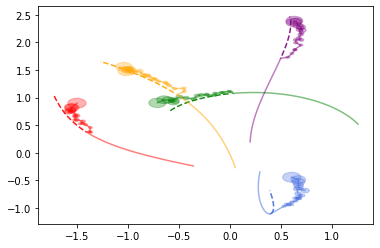
\includegraphics[width=\textwidth]{equivariance/figs/particle/lstm.png}
        \caption{LSTM}
        \label{fig:lstm}
    \end{subfigure}
    \hfill
    \begin{subfigure}[b]{0.32\textwidth}
        \centering
        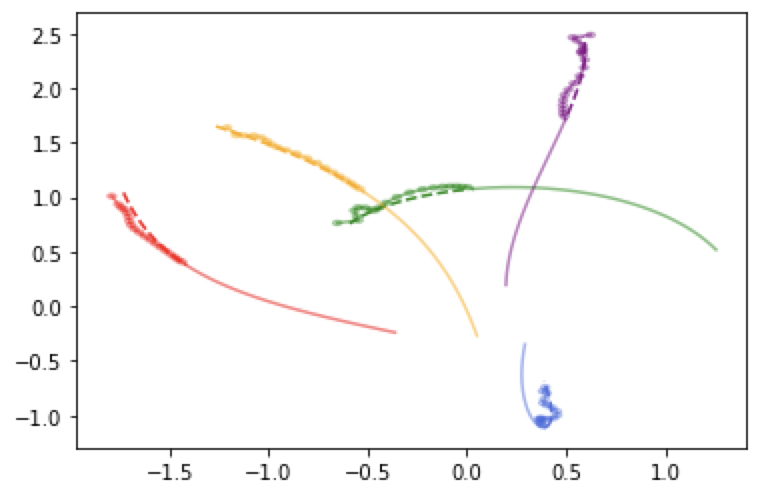
\includegraphics[width=\textwidth]{equivariance/figs/particle/ctsconv.jpg}
        \caption{CstConv}
        \label{fig:ctsconv}
    \end{subfigure}
    \hfill
    \begin{subfigure}[b]{0.32\textwidth}
        \centering
        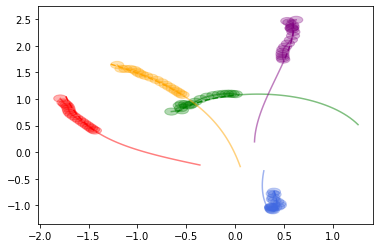
\includegraphics[width=\textwidth]{equivariance/figs/particle/pecco.png}
        \caption{PECCO}
        \label{fig:pecco}
    \end{subfigure}
    \caption{Comparison of prediction results between baselines. The solid lines are input timesteps to the models, the dotted lines ground truth, and the circles the 90\% confidence regions. We can see that PECCO achieves accurate results while maintaining good coverage.}
    \label{fig:particle}
\end{figure}


\begin{figure}[t]
\centering
\begin{subfigure}[t]{0.23\textwidth}
\centering
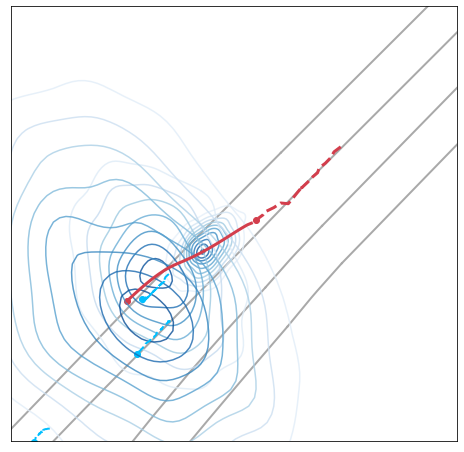
\includegraphics[width=\linewidth]{equivariance/figs/10049lstm.png}
\subcaption{LSTM-NLL}
\label{fig:sub1}
\end{subfigure}
% \begin{subfigure}[t]{0.23\textwidth}
%   \centering
%   \includegraphics[width=\linewidth]{figs/10049nll.png}
%   \subcaption{CtsConv-NLL}
%   \label{fig:sub2}
% \end{subfigure}
\begin{subfigure}[t]{0.23\textwidth}
\centering
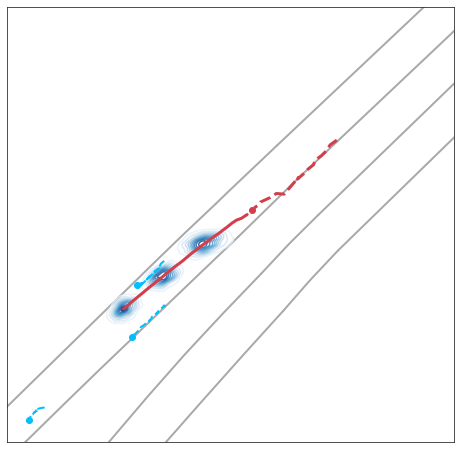
\includegraphics[width=\linewidth]{equivariance/figs/10049mis.png}
\subcaption{CtsConv-NLL}
\label{fig:sub3}
\end{subfigure}
\begin{subfigure}[t]{0.23\textwidth}
\centering
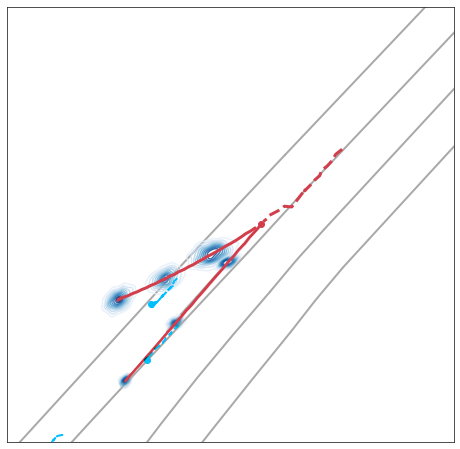
\includegraphics[width=\linewidth]{equivariance/figs/mfp.png}
\subcaption{MFP}
\label{fig:sub3a}
\end{subfigure}
\begin{subfigure}[t]{0.23\textwidth}
\centering
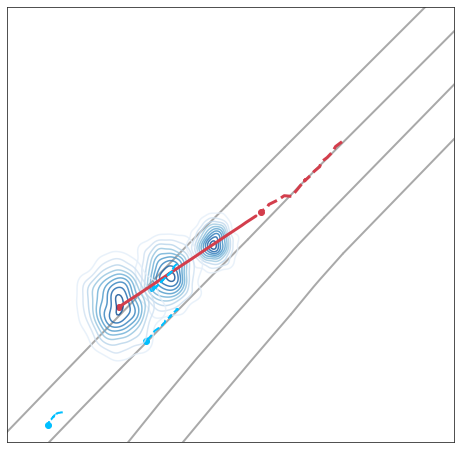
\includegraphics[width=\linewidth]{equivariance/figs/10049dyna.png}
\subcaption{PECCO}
\label{fig:sub4}
\end{subfigure}
\caption{Comparison of uncertainty predicted at a lane change. Red trajectories are the agent of interest in the same scenario. Note how the LSTM predicted uncertainty explodes after a few time steps, while CtsConv and MFP has overconfident distributions. PECCO is able to model possibility of both staying and lane change.}
\label{fig:arg-experiment}
\end{figure}

\begin{figure}
    \centering
      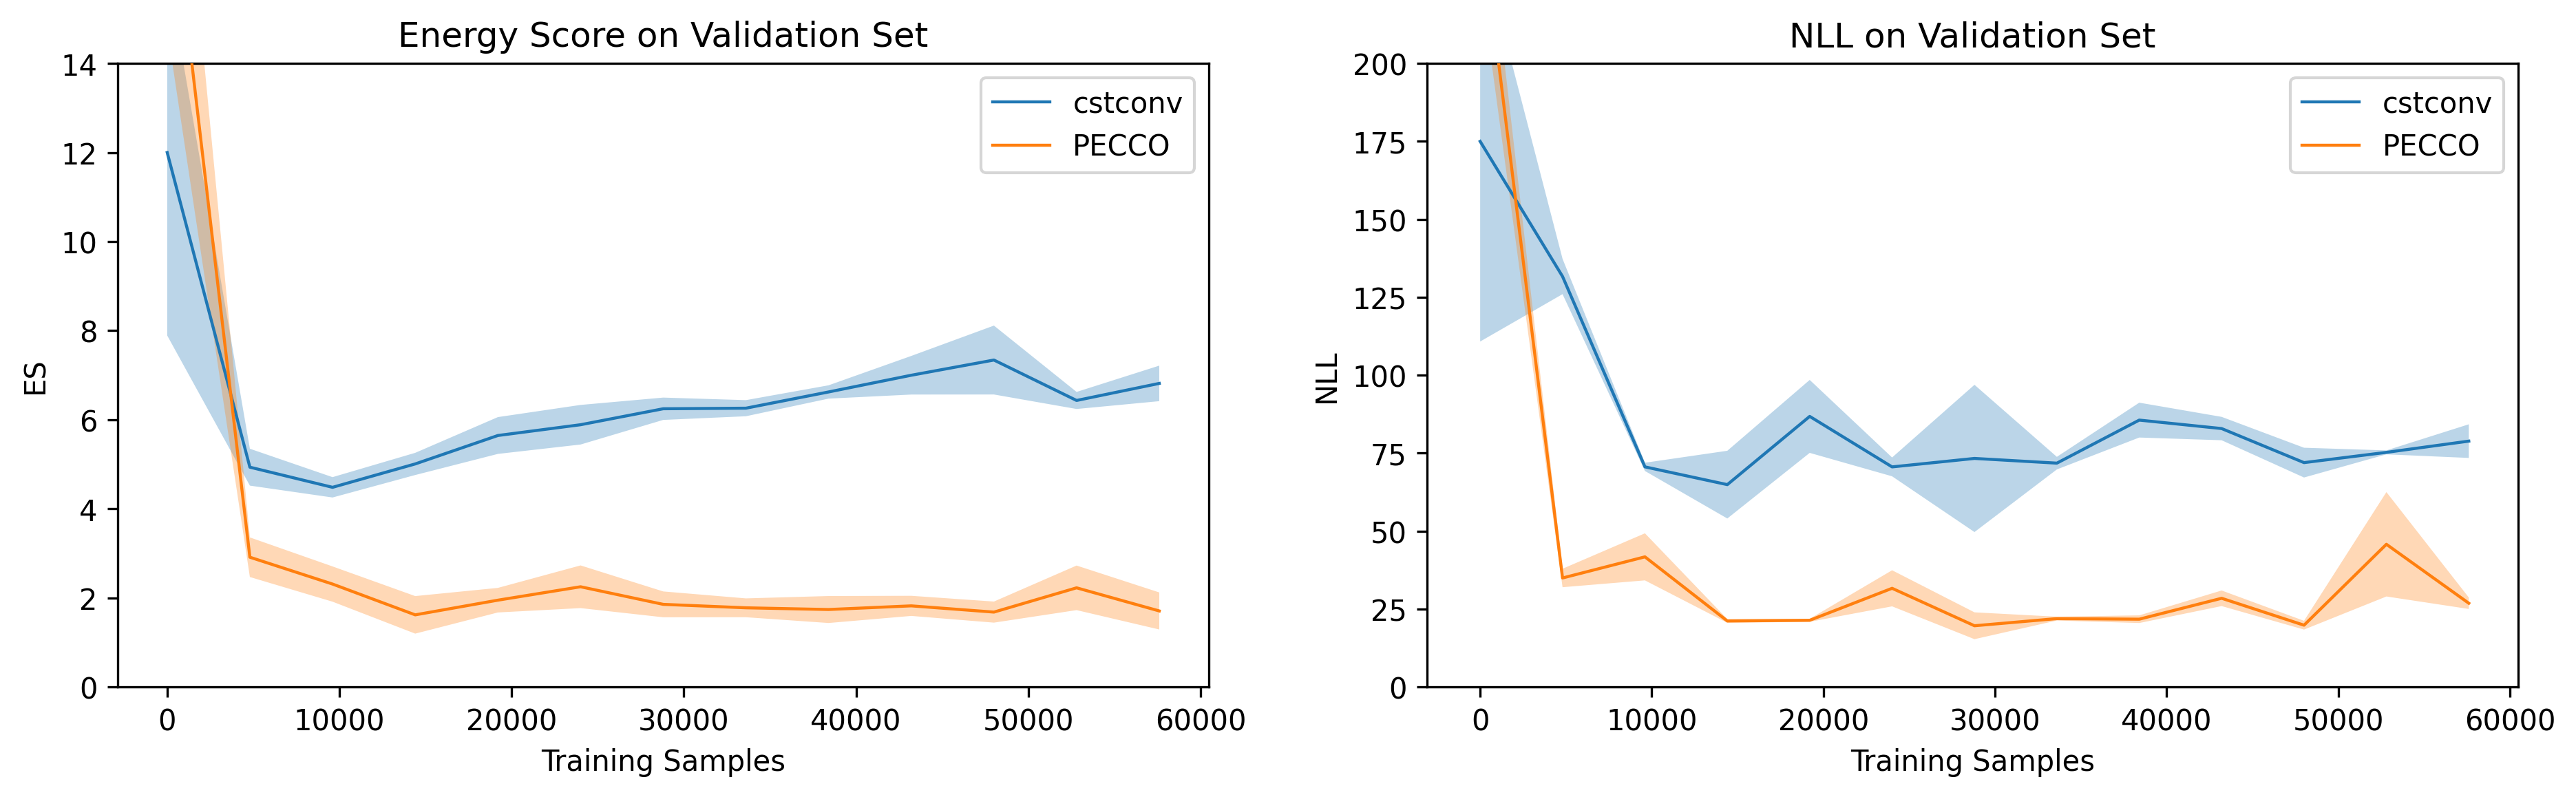
\includegraphics[width=.9\textwidth]{equivariance/figs/dataeff.png}
    \caption{With equivariance, PECCO is able to achieve better energy score and NLL with fewer data samples, compared to its non-equivariant counterpart.}
    \label{fig:dataeff}
\end{figure}

\begin{table*}[h]
\centering\resizebox{\textwidth}{!}{
\begin{tabular}{ c|c c c| ccc } 
 \toprule
  \textbf{Model} & minADE${}_6 \downarrow$ & minFDE${}_6 \downarrow$ & MRS $\downarrow$ & Cov@1s(\%) & Cov@2s & Cov@3s\\ 
\midrule
Conformal LSTM & 2.45 \plusminus{0.09}  & 4.68 \plusminus{0.15} & 198.1 \plusminus{12.0} & 90.1 \plusminus{0.1} & 92.7 \plusminus{0.1} & 92.8 \plusminus{0.1}\\
Conformal ECCO & 1.96 \plusminus{0.06} & 4.32 \plusminus{0.10} & 220.9 \plusminus{8.1} & \textbf{90.0} \plusminus{0.1} & \textbf{90.1} \plusminus{0.1} & \textbf{90.0} \plusminus{0.1} \\
\midrule
PECCO   & \textbf{1.39} \plusminus{.02}  & \textbf{3.41} \plusminus{0.03} & \textbf{8.52} \plusminus{0.16} & 74.9 \plusminus{0.2} & 93.6 \plusminus{0.8} & 92.5 \plusminus{0.9}\\
\bottomrule
\end{tabular}}
\caption{Comparison with conformal prediction methods on Argoverse dataset. PECCO produces a parametric distribution with a tighter confidence region (small MRS), whereby achieving better regression accuracy while maintaining competitive coverage.}
\label{tab:conformal}
\end{table*}


\subsection{Model Analysis}
%
\paragraph{Comparison with data augmentation and cannonicalization.}
Data augmentation and cannonicalization are popular methods to implicitly exploit symmetry in trajectory data. In Table 4 we compare PECCO to its nonequivariant counterparts with the addition of data augmentation and cannonicalization. Equivariance dramatically improves prediction performance in all aspects, especially calibration.

\begin{table}
\centering 
\begin{tabular}{ c | c c c c } 
 \toprule
  & minA/FDE$_6$ & NLL & Cov(\%) \\ 
 \midrule
  CtsConv & 1.74 / 4.43  & 29.13 & 2.2 \\
+cannon & 1.66 / 4.28 & 17.46  &  4.5  \\
+aug & 1.67 / 4.23  & 11.81  &  17.1 \\
equivariant & \textbf{1.39} / \textbf{3.41} & \textbf{4.26}  & \textbf{87.5} \\
\bottomrule
 \end{tabular}
\caption{Data Augmentation Comparison on the Argoverse Dataset.}
\label{tab:aug-ablation}
\end{table}

\paragraph{Dynamics Integration Ablation.}
Dynamic integration (dyna) introduced in Section \ref{sec:dyn_inte} enforces the uncertainty to grow monotonically over time. As an ablative study, Table 5 show that PECCO with  dynamic integration has much better calibration compared to if without; for the Argoverse dataset, the improved calibration also informs better performance on minADE/FDE.

\begin{table}
\centering 
\begin{tabular}{ c|c c c  } 
\toprule
\textbf{Argoverse} & minA/FDE$_6$ & NLL & Cov(\%) \\ 
\midrule
no-dyna & 1.52 / 3.76 & 9.72  & 38.6 \\
dyna & \textbf{1.39} / \textbf{3.41} & \textbf{4.26}  &  \textbf{87.5} \\
\toprule
\textbf{Pedestrian} & minA/FDE$_6$ & NLL & Cov(\%) \\ 
\midrule
no-dyna & \textbf{0.72} / 2.12 & 4.71 & 39.6  \\
dyna & 0.73 / \textbf{1.98} & \textbf{2.37}  & \textbf{83.7} \\
\bottomrule
\end{tabular}
\caption{Dynamics Integration (dyna) Ablation: using dyna encourages the uncertainty to grow over time and improves coverage.}
\label{tab:dynamics-ablation}
\end{table}


\paragraph{Comparison with Conformal Prediction.}
%Conformal prediction is a uncertainty quantification method with theoretical guarantees on coverage without imposing any assumptions about the underlying distribution.
We compare to two conformal prediction baselines \cite{2021conformal} (Appendix \ref{app:conformal} for details) in Table 3. Conformal methods achieve guaranteed $\geq 90\%$ coverage, but suffer in prediction accuracy due to having to split training data for calibration. Since conformal prediction does not output a distribution, we use another proper scoring rule Mean Regional Score (2d extension of mean interval score in \cite{properscoring}, see Appendix B) as metric. The conformal regions are much larger (higher MRS), which is less desirable for downstream decision making tasks.
%see appendix \ref{app:conformal} for details and qualitative visualization.
\section{Conclusion}
In this work we propose Probabilistic Equivariant Continuous Convolution (PECCO),  a novel  multi-agent probabilistic prediction method for improving uncertainty quantification. We design an equivariant neural network under which the predicted distributions transform correspondingly as inputs are transformed. We introduce the Energy Score metric to bring attention to the calibration of multivariate probabilistic forecasts. By leveraging equivariance, PECCO produces more accurate and calibrated probabilistic forecasts compared to existing methods on both synthetic and real-world datasets.
%A future direction of this work is to expand PECCO to produce multimodal forecasts. In this paper, we made the simplifying assumption that the uncertainties are 2-D normal distributions. By modifying PECCO to output a mixture of Gaussian, we can describe more complex trajectory distributions.


% Acknowledgments---Will not appear in anonymized version
%\acks{This work was supported in part by U.S. Department Of Energy, Office of Science, Facebook Data Science Research Awards, U. S. Army Research Office under Grant W911NF-20-1-0334, and NSF Grants \#2134274 and \#2146343. }

\pagebreak

\section{Proofs}
\label{app:equiv_dist}

\subsection{Proofs for Equivariance of Gaussians [Proposition \ref{prop:equivnormal}]}

In this section, we prove that the Gaussian probability density function is $\SOtwo$-equivariant.

\begin{prop*}
 Given multivariate normal distribution $\mathcal{N}(\mu,\Sigma)$ over $\mathbb{R}^2$ with probability density function $p_{\mu, \Sigma}$ and $g\in \SOtwo$, then $p_{g\mu, g\Sigma g^T} (v) = p_{\mu, \Sigma} (g^{-1}v)$ for all $v \in \mathbb{R}^2$.
\end{prop*}

\begin{proof}
\begin{align*}
P_{g\mu, g\Sigma g^T}(v) &= \frac{1}{2 \pi \det{(g\Sigma g^T)}} \exp{(-\frac{1}{2}(v-g\mu)^T (g \Sigma g^T)^{-1} (v - g\mu))} \\
 &= \frac{1}{2\pi \det{(\Sigma})} \exp{(-\frac{1}{2}(g^{-1}v-\mu)^T g^T g^{-T} \Sigma^{-1} g^{-1} g (g^{-1}v -\mu))} \\
&= \frac{1}{2\pi \det{(\Sigma})} \exp{(-\frac{1}{2}(g^{-1}v-\mu)^T \Sigma^{-1} (g^{-1}v -\mu))}\\ 
&= P_{\mu, \Sigma}(g^{-1}v) 
\end{align*}
\end{proof}


\begin{prop*} 
Given a normal distribution $\mathcal{N}(\mu,\Sigma)$, its group-actioned $\mathcal{N}(g\mu, g\Sigma g^T)$ is also a valid normal distribution. 
\end{prop*}

\begin{proof}
We prove the proposition by proving that $g\Sigma g^T$ is a symmetric positive definite matrix.

1) \textit{(Symmetry)} $(g\Sigma g^T)^T = g^{TT} \Sigma^T g^T = g\Sigma g^T$.

2) \textit{(Positive Definite)}  Let $v\in \mathbb{R}^2 $ and $v\neq 0$. Let $w = g^T v$, note that $w\neq 0$. Then $v^T g\Sigma g^T v =  w^T \Sigma w >0$, which implies $\Sigma$ is a positive definite matrix.  
\end{proof}

\subsection{Equivariance of construct for positive definite and symmetric $\Sigma$ [Proposition \ref{prop:pds}]}

%We want a neural network $f$ such that $z \xrightarrow[]{f} \mu, \Sigma$. $\mu$ is a $\rho_1$ feature. 

Note that every positive definite symmetric matrix can be written as $\Sigma = MM^T$ for some $M\in GL_2(\mathbb{R})$, so we can represent $\Sigma$ by a map $\varphi$ where
\begin{align*}
       \varphi \colon \mathrm{GL}_2(\mathbb{R}) &\to \mathrm{PosDefSym}_2(\mathbb{R})  \\ 
    M &\mapsto M M^T
\end{align*}

\begin{prop*}
$\varphi$ is $\SOtwo$-equivariant.
\end{prop*}
\begin{proof}
$\varphi (gMg^T) = gMg^T (gMg^T)^T = gMg^T g^{TT} M^T g^T = gMM^Tg^t = g\varphi(M)g^T $
\end{proof}

We defined the one-sided inverse of $\varphi$ as $\psi$:
\begin{align*}
        \psi \colon \mathrm{PosDefSym}_2(\mathbb{R}) &\to \mathrm{GL}_2(\mathbb{R})    \\ 
        \Sigma &\mapsto Q \lambda^{\frac{1}{2}}
\end{align*}
where $Q\lambda Q^T$ is the eigendecomposition of $\Sigma$ and $Q$ is orthogonal.   That is, $\varphi (\psi(\Sigma)) = \Sigma$.
\begin{prop*}
$\psi$ is $\SOtwo$-equivariant.
\end{prop*}
\begin{proof}
For symmetric positive definite matrix $\Sigma$, its eigenvector $v_i$ and eigenvalue $\lambda_i$ follows the eigenequation
\[
    \Sigma v_i = \lambda_i v_i .
\]
For $\forall g \in \SOtwo$, 
\[
  g\Sigma v_i = \lambda_i g v_i \implies g\Sigma g^{-1} g v_i = \lambda_i g v_i \implies (g\Sigma g^{-1}) (g v_i) = \lambda_i (g v_i) ,
\]
so $gv_i$ is an eigenvector to $g\Sigma g^{-1}$, with corresponding eigenvalue $\lambda_i$.

Therefore, 
\[
\psi (g\Sigma) = gQ\Lambda^{\frac{1}{2}} = g\psi (\Sigma).
\]
\end{proof}

% \subsection{Equivariance for Quadratic Form}
% Two n-ary quadratic forms $\phi$ and $\psi$ over $\R$ are equivalent if there exists a nonsingular linear transformation $M \in GL(n)$ such that $\phi(x) = \psi (Mx), \forall x\in \R^n$. Under the equivalence $M$, the symmetric matrix $A$ of $\phi$ and the symmetric matrix $B$ of $\psi$ are related by a change of bases: $A = M^TBM$.

% \begin{prop*}
% Given $\SOtwo$-equivariant neural network $f_1:\R^2\rightarrow \R^2$ and $f_2:\R^2\rightarrow \R^2$, for all non-zero $\rho_1$ feature $h \in \R^2$, defining the linear transformation $M(h) = [f_1(h), f_2(h)]$, the symmetric matrix $\Sigma(h) = M(h)M(h)^T$ for the corresponding quadratic form is equivariant.
% \end{prop*}
% \begin{proof}
% \begin{align*}
%     C(gh) & = M(gh)M(gh)^T = 
%     \begin{bmatrix} f_1(gh) & f_2(gh)\end{bmatrix}
%     \begin{bmatrix} f_1(gh)^T \\ f_2(gh)^T\end{bmatrix} \\
%     & = \begin{bmatrix} gf_1(h) & gf_2(h)\end{bmatrix}
%     \begin{bmatrix} f_1(h)^Tg^T \\ f_2(h)^Tg^T\end{bmatrix} \\
%     & = g\begin{bmatrix} f_1(h) & f_2(h)\end{bmatrix}
%     \begin{bmatrix} f_1(h)^T \\ f_2(h)^T\end{bmatrix}g^T \\ 
%     & = gM(h)M(h)^Tg^T = g\Sigma(h)g^T
% \end{align*}
% \end{proof}

% Since the covariance matrix $\Sigma$ is a positive definite symmetric matrix, it defines a quadratic form over $\R$. For non-zero $\rho_1$ feature $h \in \R^2$, we can define $\Sigma(h) =  M(h)M(h)^T$. Then the defined quadratic form $x^T\Sigma x$ is equivalent to standard quadratic form $x^Tx$ under equivalence $M(h)$, and this equivalence is equivariant. In other words, the neural network changes the bases of identity matrix equivariantly for covariance matrix.



\subsection{Proof of Proposition \ref{prop:equivtoinvar}: The Equivariant Model Gives an Invariant Conditional Distribution. }


We now prove Proposition \ref{prop:equivtoinvar}.

\begin{prop*}[Proposition \ref{prop:equivtoinvar}]
If the one-step probabilistic forecasting model $f_\theta$ is $G$-equivariant, then the conditional probability distribution $p_\theta( \mathbf{x}_{t+1:t+k} | \mathbf{x}_{1:t}, \mathbf{e})$ is invariant as in \autoref{eqn:invariant_prob}.
\end{prop*}

\begin{proof}
Since $\mathbf{x}_{1:t}$ are known, we define $\Sigma_{1:t} = \epsilon \mathrm{Id}$ for $\epsilon$ small approximating a delta distribution at $\mu_{1:t} = \mathbf{x}_{1:t}$.
We then evaluate $\mu_{j+1},\Sigma_{j+1} = f_\theta(\mu_{j-t+1:j}, \Sigma_{j-t+1:j}, \mathbf{e})$ autoregressively for $j=1,\ldots,k$.  Finally define 
\begin{equation}
\begin{aligned}
    p_\theta( \mathbf{x}_{t+1:t+k} | \mathbf{x}_{1:t}, \mathbf{e}) &=
    \prod_{j=1}^k  p_\theta( \mathbf{x}_{t+j} | \mathbf{x}_{j:t+j-1}, \mathbf{e}) \\
    &= \prod_{j=1}^k p_{N(\mu_{t+j},\Sigma_{t+j})}(\mathbf{x}_{t+j}). 
\end{aligned}
\label{eq:timeseriespdf}
\end{equation}

For $g \in \SOtwo$, we want to show 
\[
    p_\theta( g\mathbf{x}_{t+1:t+k} | g\mathbf{x}_{1:t}, g\mathbf{e}) = p_\theta( \mathbf{x}_{t+1:t+k} | \mathbf{x}_{1:t}, \mathbf{e}).
\]
  Thus for $g\mathbf{x}_{1:t}, g\mathbf{e}$ we initialize $g \mu_{1:t},g\Sigma_{1:t}g^{T}$ since $g\Sigma_{1:t}g^T = gg^T\Sigma_{1:t}= \Sigma_{1:t}$. Applying $f_\theta$ repeatedly and invoking equivariance, we obtain 
\begin{align}
    g\mu_{t+j},g\Sigma_{t+j}g^{T} = f_\theta(g\mu_{j:t+j-1}, g\Sigma_{j:t+j-1}g^{T}, g\mathbf{e}). 
\end{align}
for $j =1,\ldots,k$.  Then by \autoref{eq:timeseriespdf}, 
\[
    p_\theta( g\mathbf{x}_{t+1:t+k} | g\mathbf{x}_{1:t}, g\mathbf{e}) =
    \prod_{j=1}^k p_{N(g\mu_{t+j},g\Sigma_{t+j}g^{T})}(g\mathbf{x}_{t+j}).
\]
Then by Proposition \ref{prop:equivnormal} this is 
\[
  \prod_{j=1}^k p_{N(\mu_{t+j},\Sigma_{t+j})}(g^{-1}g\mathbf{x}_{t+j}),
\]
which cancels $g^{-1}g = 1$, and applying \autoref{eq:timeseriespdf} again gives  $p_\theta( \mathbf{x}_{t+1:t+k} | \mathbf{x}_{1:t} \mathbf{e})$.  
\end{proof}



\subsection{Proof that MRS is a strictly proper scoring rule}
\label{app:properscoring}

Scoring rules are summary measures to evaluate probabilistic forecasts; they take in the forecasted distribution and the event or value that materializes and assign a numerical score. As defined in \cite{properscoring},  a scoring rule is proper if it is maximized when the forecaster recovers the ground truth distribution. It is strictly proper if the maximum is unique.

\begin{prop*} 
MRS is a strictly proper score.
\end{prop*}
\begin{proof}
%For arbitrary predictive distributions $P$ and $Q \in \mathbb{R}$, $MRS(P,Q) \geq 0$. Moreover, $MRS(P,Q) = 0$ holds if and only if $P=Q$.
For arbitrary function $h$, we first define the scoring rule
\[
 S(R;z) = -|R| + \frac{1}{\alpha}(|R| - |R(z)|)\mathbb{1}\{z\in R^C\} + h(z),
\]
which means if the forecaster quotes region $R$ at the level $\alpha\in (0,1)$ and $z$ materializes, then the score $S(R;z)$ will be rewarded, where $R$ and $R(z)$ are defined as ellipsoid parametric by $\mu$ and $\Sigma$. Then the expected score under the probability measure $P\in \mathcal{P}$ which $z$ follows is defined as
\[
 S(R;P) = \int S(R;z) \, dP(z). 
\]
For $P\in \mathcal{P}$, let $R_*$ denote the unique true $P$-region at level $\alpha$. We say that scoring rule $S$ is strictly proper if 
\[
 S(R_*;P) \geq S(R;P),
\]
for all region $R$ and for all probability measures $P\in \mathcal{P}$, where equality holds if and only if $R = R_*$. 

We identify $P$ with the associated distribution function so that $P(R_*^C)=\alpha$. If $R_* \subset R$, then
\begin{align*}
    S(R_*;P) - S(R;P) & = \int -|R_*| \, dP(z) + \frac{1}{\alpha} \int_{R_*^C} (|R_*| - |R(z)|) \, dP(z) \\
    & + \int |R| \, dP(z) - \frac{1}{\alpha} \int_{R^C} (|R| - |R(z)|) \, dP(z) \\
    & = -|R_*| + |R| + \frac{1}{\alpha}|R_*|P(R_*^C) - \frac{1}{\alpha}|R|P(R^C) - \frac{1}{\alpha}\int _{R_*^C \setminus R^C} |R(z)| \, dP(z) \\
    & \geq |R| - \frac{1}{\alpha}|R|P(R^C) - \frac{1}{\alpha}|R|(P(R_*^C)-P(R^C)) \\
    & = 0, 
\end{align*}
as it is supposed to be. If $R \subset R_*$, then an analogous argument applies. 

Putting $h(z) = 0$ and reversing the sign of the scoring rule, yields the negatively oriented regional score. Finally, the mean score of this oriented regional score is our MRS, which is then proved to be proper.
\end{proof}


\section{Supplementary: Equivariant Matrix Output Layer Construction}
\label{app:matrix}

Let 
\[
    \rho_1(\theta) = \begin{pmatrix}
    \cos{\theta} & -\sin{\theta} \\
    \sin{\theta} & \cos{\theta}
    \end{pmatrix} 
    \qquad\qquad
        M = \begin{pmatrix}
    a & b \\
    c & d
    \end{pmatrix}
\]
where $a,b,c,d$ are trainable parameters.
Consider input $f \colon S^1 \to \mathbb{R}$, then
\[
F(f) = \int_{\theta=0}^{2\pi} f(\theta) \rho_1(\theta) M \rho_1(-\theta) d\theta.
\]
Define $\rho_{reg}(\phi)(f)(\theta) = f(\theta-\phi)$.  
\vspace{5px}
\begin{prop*}
The convolution $F$ is equivariant, i.e.,
\[
F(\rho_{reg}(\phi) f) = \rho_1(\phi) F(f) \rho_1(-\phi).
\]
\end{prop*}
\begin{proof}
We compute
\begin{align*}
    F(\rho_{reg} (\phi)f) 
    &= \int_{\theta=0}^{2\pi}  \rho_{reg}(\phi)(f)(\theta) \rho_1(\theta) M\rho_1(-\theta) d \theta \\
    &= \int_{\theta=0}^{2\pi}  f(\theta-\phi) \rho_1(\theta) M\rho_1(-\theta) d \theta \\
    &= \int_{u=-\phi}^{2\pi-\phi} f(u) \rho_1(u+\phi)M\rho_1(-u-\phi)du \quad (\text{substituting } u = \theta - \phi) \\ 
% \end{align*}
% Since the integrand is periodic, this is equal to integrating from $u=0$ to $u = 2\pi,$ 
% \begin{align*}
    &= \rho_1(\phi) \cdot \left( \int_{u=-\phi}^{2\pi-\phi} f(u) \rho_1(u)M\rho_1(-u)du \right) \cdot \rho_1(-\phi) \\
    &=  \rho_1(\phi) F(f) \rho_1(-\phi). 
\end{align*} 
The last substitution follows from the fact the integrand is periodic of period $2\pi$. Since the integral is over the whole circle, this equal to taking the limits of integration to be $0$ and $2\pi$.
\end{proof}

\vspace{3px}

\paragraph{Discritization.}
If the function $f$ is discretized, such that $f_i = f(i2\pi/n)$.  Then the mapping $F$ is given by 
\[
F(f) = \sum_{i=0}^{n-1} f_i \rho_1(i2\pi/n) M \rho_1(-i2\pi/n).
\]

\paragraph{Compatibilitiy with matrix exponential}

For a $n \times n$ matrix $M$ define 
\[
\exp(M) = \sum_{k=0}^\infty M^k/k!.
\]
Matrix exponentiation is equivariant with respect to conjugation.  That is for $g \in \mathrm{GL}_n(\mathbb{R})$, 
\[
\exp(gMg^{-1}) = \sum_{k=0}^\infty (gMg^{-1})^k/k!. 
\]
Now note that
\[
(gMg^{-1})^k = (gMg^{-1}) (gMg^{-1}) \ldots (gMg^{-1}) = gMM \ldots Mg^{-1} = g M^k g^{-1}.
\]
So then 
\[
\sum_{k=0}^\infty (gMg^{-1})^k/k! = \sum_{k=0}^\infty gM^kg^{-1}/k! = g \left( \sum_{k=0}^\infty M^k/k! \right) g^{-1} = g \exp(M) g^{-1}.
\]

\paragraph{Structured Network Output}

So the last layers of the neural network will be $\exp \circ F$ which outputs an invertible $2 \times 2$ matrix and satisfies 
\[
(\exp \circ F)(\rho_{reg}(\phi) f) = \rho_1(\phi) (\exp \circ F)(f) \rho_1(-\phi).
\]


\section{Supplementary: Baseline Algorithms}

\subsection{Score Function for Probabilistic Forecast}
% \subsection{Problem Formulation}

We consider a probabilistic approach to trajectory forecasting. Ideally, we want the predicted distribution to be both sharp and valid under the definition in \Eqref{eq:coverage}. To quantify the uncertainty, we review the classic score function Mean Interval Score (MIS) and derive a 2 dimensional extension, Mean Regional Score (MRS).

% \leo{Is 'interval' a proper terminology here? Empirically it's a 1-d concept, for n-d interval people always mean region with square bounding. It's confusing especially when the mean interval score below is a 1-d metric.} 

% For each agent in the scene, we estimate a sequence of $k$ prediction regions $\Hat{C}_{t+1:t+k}$ for $\mathbf{x}_{t+1:t+k}$. The intervals $\Hat{C}$ are dependent on a significance level $\alpha$, denoted  as $\Hat{C}^{\alpha}$. 

% given by $p_\theta( \mathbf{x}_{t+1:t+k} | \mathbf{x}_{1:t}, \mathbf{e})$,


\paragraph{Mean Interval Score.}
Mean Interval Score (MIS) is a proper scoring rule \cite{properscoring} for interval forecasts that rewards narrower confidence intervals and encourages coverage. 
%
Specifically, let $Y  \sim {P}_Y$ be a one-dimensional random variable, and an upper bound $u$, a lower bound $l$ be its estimated $\frac{\alpha}{2}$ and $(1-\frac{\alpha}{2})$ quantiles respectively, MIS is defined using samples $y_i \sim {P}_Y$.
 %
\begin{align}
    \mathrm{MIS}(u,l; Y) = \frac{1}{N} \sum_{i=1}^{N}[(u-l) +
     \frac{2}{\alpha}(y_i-u)\mathbb{1}\{y_i>u\}\nonumber 
     + \frac{2}{\alpha}(l-y_i)\mathbb{1}\{y_i<l\} ] 
    \label{eq:mis}
\end{align}
%
Where the three terms in  \Eqref{eq:mis} accounts for the width of the interval, and how much the sample point exceeds the upper bound and the lower bound, respectively. MIS has the advantage of being easy to compute and does not require the model to be parametric \cite{properscoring}. It can also be used as an objective function for probabilistic forecasting \cite{wu2021quantifying}. 


\paragraph{Mean Regional Score.}
For n-D distributions, we introduce a new metric called the Mean Region Score (MRS), which generalizes MIS to higher dimensions. 
%
Let $Z \sim {P}_Z$ be an n-dimensional continuous random variable. First, we need to generalize  $\alpha$-quantile and define the  confidence region. Let the region bordering $z$ as $R(z)$, the  confidence region of level $\alpha$ 
\begin{align}
R_P(\alpha) =  \inf \lbrace R(z)  | \int_{R(z)} P( z ) dz \geq \alpha \rbrace
\end{align}
is the smallest region whose probability exceeds  level $\alpha$.

\begin{figure}
    \centering
  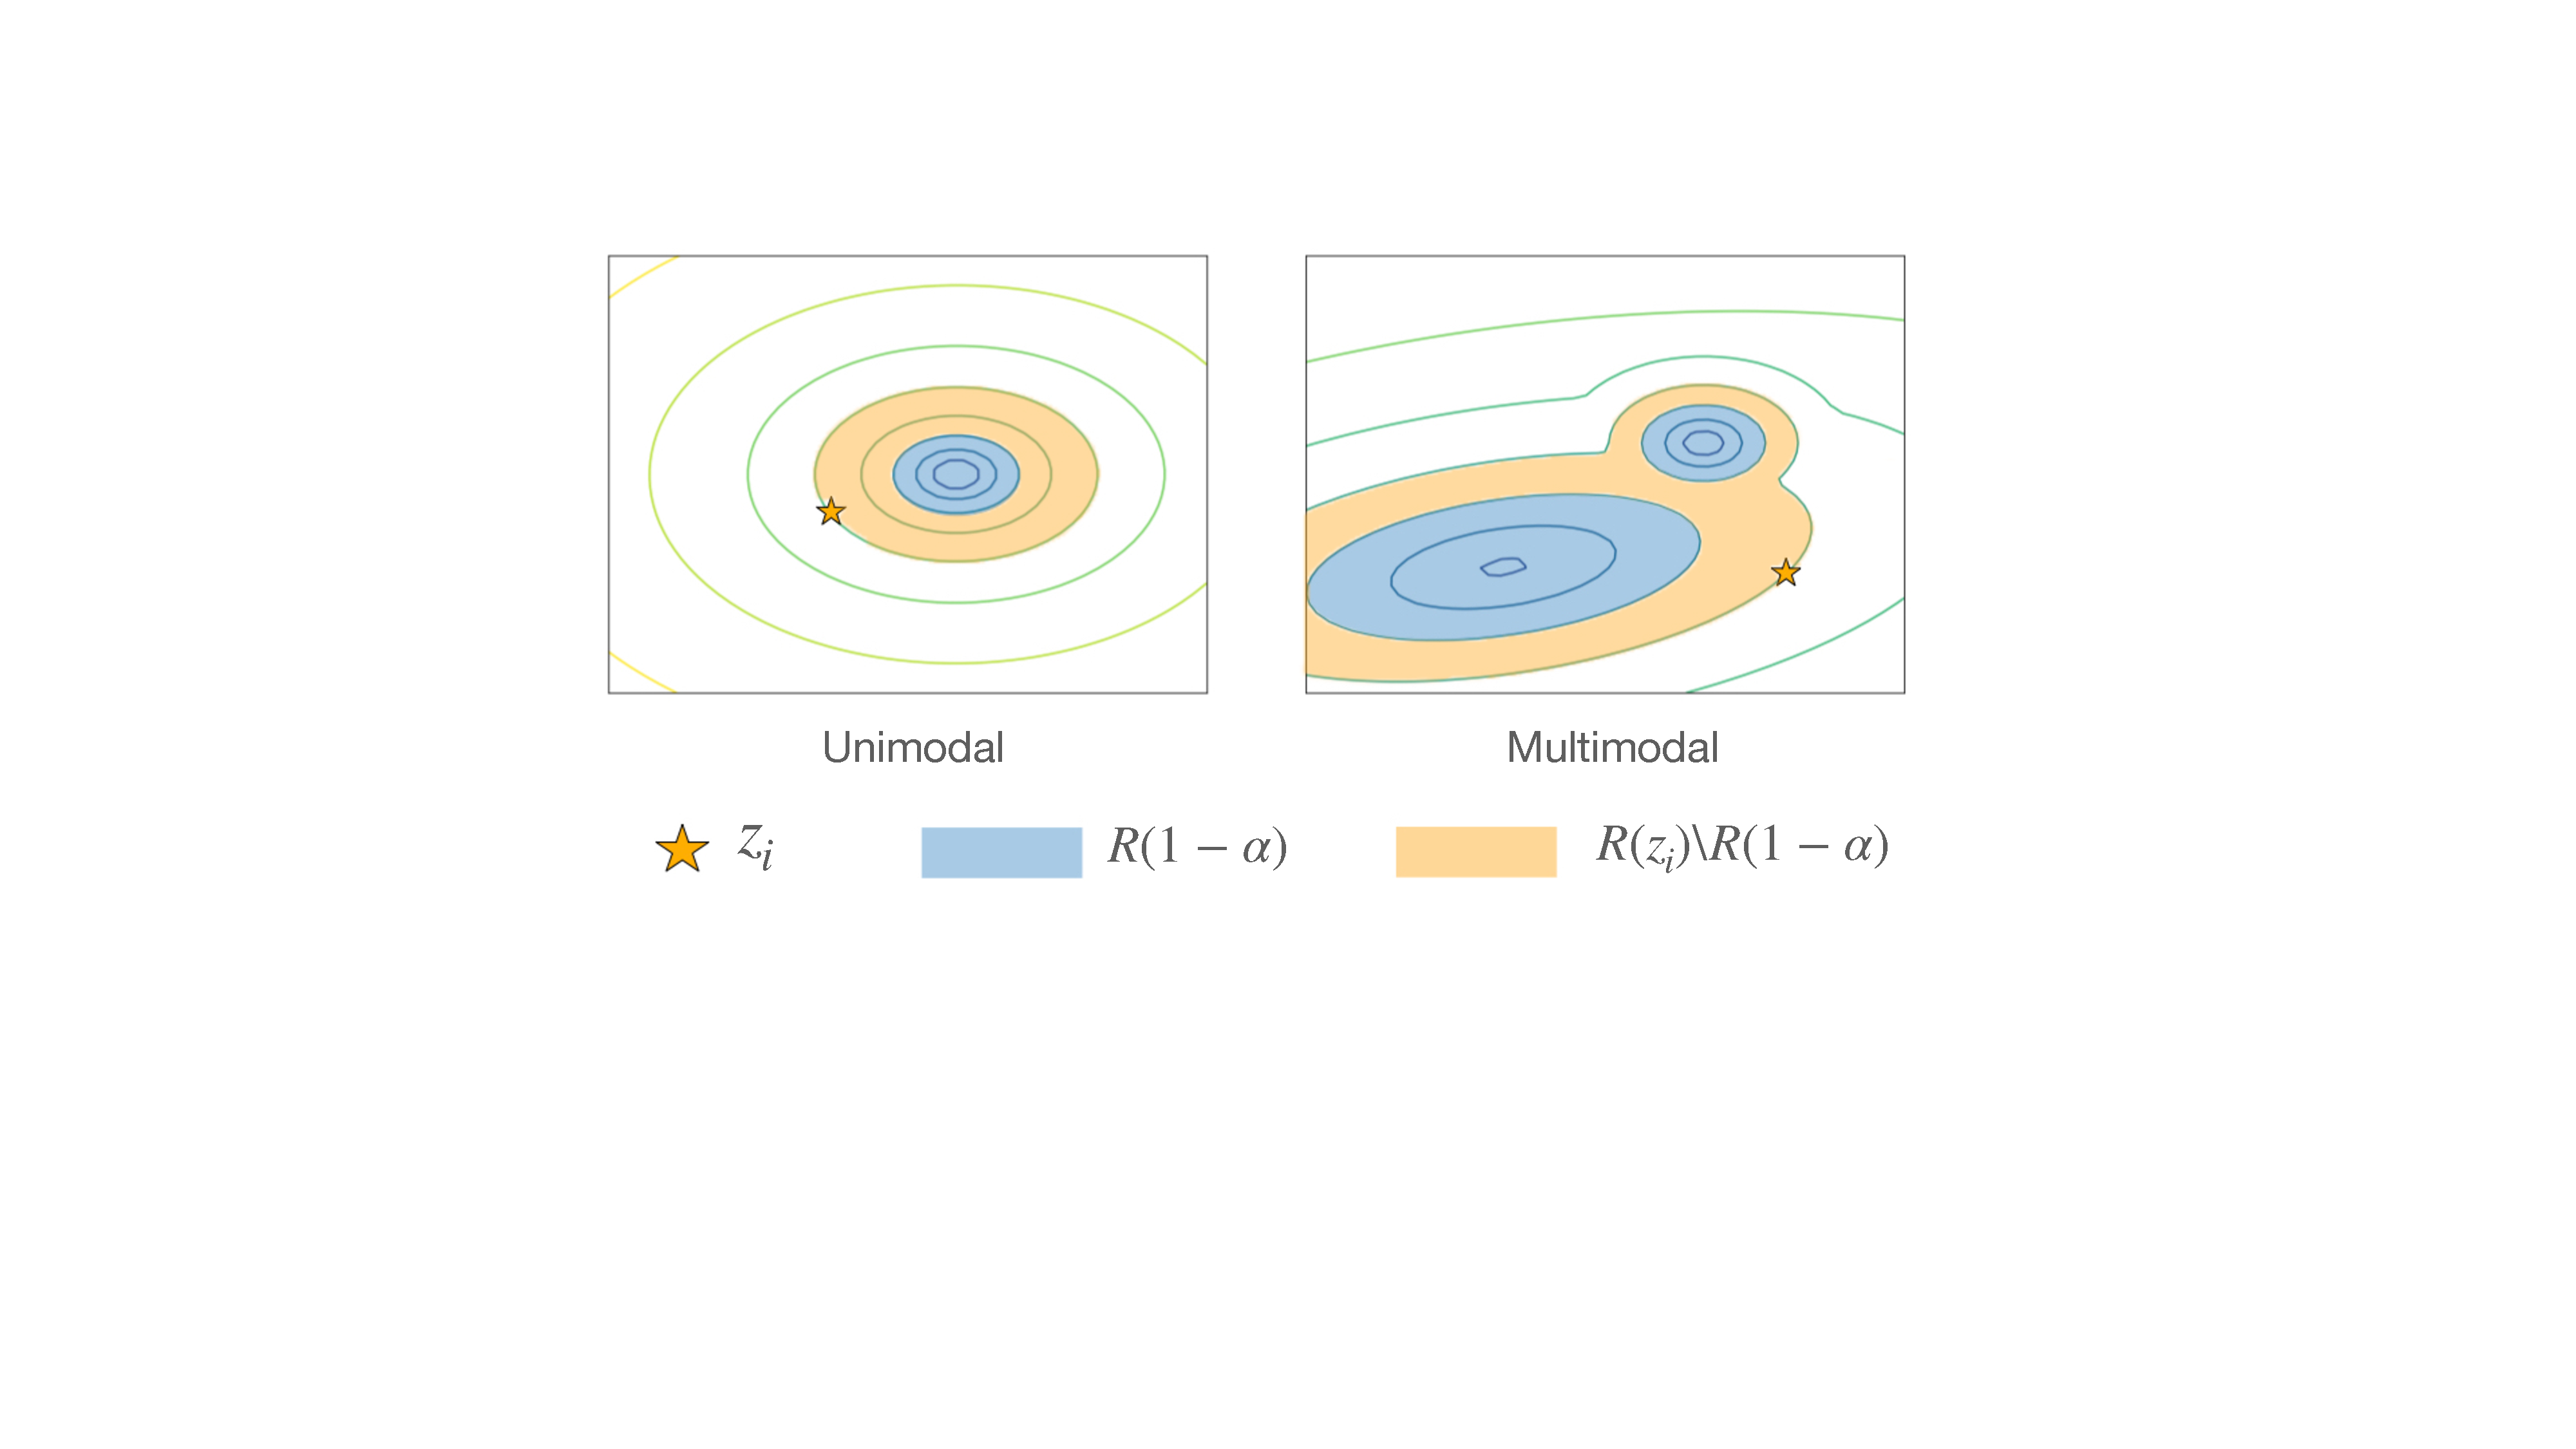
\includegraphics[width=.8\linewidth]{equivariance/figs/mrs.pdf}
  \caption{MRS illustration for   unimodal and multimodal distributions. Given a sample $z_i$, MRS  calculates the area of blue region plus that of the the orange region scaled by $1/\alpha$. }
  \label{fig:mrs}
\end{figure}
When the distribution is Gaussian $P_Z =\mathcal{N}(\mu, \Sigma)$ with mean $\mu \in \mathbb{R}^n$ and the covariance matrix $\Sigma \in \mathbb{R}^{2\times 2}$ that is positive definite. The $(1-\alpha)$ confidence region of an n-D multivariate normal distribution $P = \mathcal{N}(\mu, \Sigma)$ is an ellipsoid that can be written as \cite{slotani1964tolerance}:
\[
    R(1-\alpha) = \{ z| (z-\mu)^T \Sigma^{-1} (z-\mu) \leq  \chi_n^2(1-\alpha)\}.
\]
where $\chi_n^2$ is the chi-squared distribution with n degrees of freedom.
Then, for a given sample $z_i \in \mathbb{R}^n$, we can draw an ellipsoid whose edge coincides $z_i$ defined as 
\[
    R(z_i) = \{z|(z-\mu)^T\Sigma^{-1}(z-\mu) \leq c'\} 
\]
where $c' = (z_i - \mu)^T \Sigma^{-1} (z_i - \mu)$.


% The smallest confidence region of  $1-\alpha$ could be viewed as a superlevel set of points with probability greater than a threshold $\zeta_{1-\alpha}$. \cite{multimodalconfidence}




The MRS score of the $(1-\alpha)$ prediction interval thus can be evaluated as:
%
\begin{align}
    \mathrm{MRS}(R ;Z) = \frac{1}{N} \sum_{i=1}^N  [|R(1-\alpha)| +   \frac{1}{\alpha}| R(z_i) \backslash R(1-\alpha)| \mathbb{1} \{z_i \in R^C(1-\alpha)\}]
\label{eq:mrs}
\end{align}
where the first term  corresponds to the area of the confidence region and the second term measures how much each data $z_i$ deviates from the region. $|\cdot|$ measures the size of the set.  It is also easy to prove (see Appendix \ref{app:properscoring}) that MRS is a proper scoring rule \cite{properscoring}, which means MRS is optimized if and only if the distribution $P$ recovers that of $Z$.

Figure \ref{fig:mrs} illustrates MRS for both unimodal and multimodal distributions.  Note that when the distribution is single-modal, the confidence interval in \Eqref{eq:mrs} is both \textit{equally tailed} and the \textit{shortest} confidence interval. For  multi-modal distributions,  we solve for the \textit{smallest} confidence region to cover probable events. In appendix \ref{app:mrsgeneral} we present a method to estimate MRS for arbitrary 2-D distributions, where we divide the domain space into small grids to estimate density, and obtain $R(1-\alpha)$ and $R(z_i)$ by assembling high density regions.
%


%For an arbitrary distribution $P$ over $\mathbb{R}^2$, we can define the confidence region $S_P$ as the superlevel set $S_P(1-\alpha) = \lbrace x \in \mathbb{R}^2 | p(x) \geq c(\alpha) \rbrace$, where $c(\alpha)$ is defined such that 

\subsection{Empirical method for estimating MRS for general 2D distribution }
\label{app:mrsgeneral}

We present an empirical method to estimate MRS given any 2D distribution. We first discretize the 2D space that is the domain of the probability distribution into $n$ grid cells, indexing them as $g_i$ where $i\in \{1,\ldots,j\}$. Then we can numerically estimate the density of each grid cell $p(g_i)$ for $i= 1,\ldots,n$. The confidence region can be estimated by selecting the grid cells with the highest likelihoods until they sum to $1-\alpha$. 
\[
R(1-\alpha) = \bigcup_{i\in K} g_i, \quad K =  \text{argmin}_K: \Sigma_{i\in K} p(g_i) \geq 1-\alpha
\]
where $K$ is the superlevel set of grid cells $g_i$ whose empirical probability density is at least  $1-\alpha$.

Similarly, we define the estimated region 
\[ 
R (z_i) = \bigcup g_i \quad \text{ for } p(g_i) \geq p(z_i)
\]
as the superlevel set of data point $z_i$. This way, we can calculate MRS for any 2D using the estimated $R(1-\alpha)$ and $R(z_i)$ in the MRS formula. 
\[
    \mathrm{MRS}(R ;Z) = \frac{1}{N} \sum_{i=1}^N  [|R(1-\alpha)| +     \frac{1}{\alpha}| R(z_i) \backslash R(1-\alpha)| \mathbb{1} \{z_i \in R^C(1-\alpha)\}]
\]

Figure \ref{fig:empiricalmrs} illustrates the idea, this method is used to estimate the MRS scores for multimodal methods \texttt{Trajectron++} and \texttt{MFP} in our experiments.

\begin{figure}[!h]
  \centering
  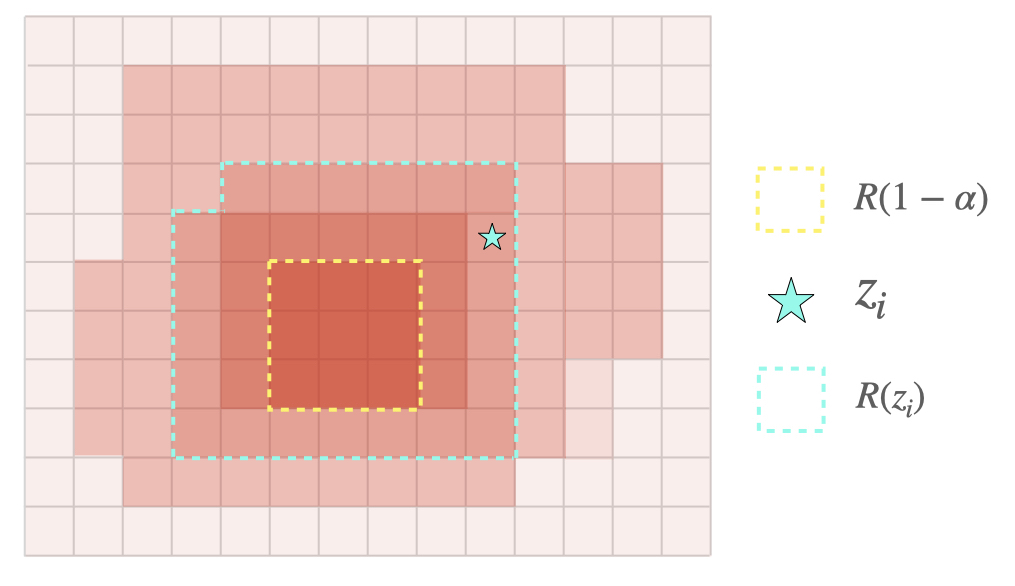
\includegraphics[width=.5\linewidth]{equivariance/figs/empmrs.jpeg}
  \caption{Illustration for empirical MRS estimation, where we calculate the probability density at each grid, and select the highest density grids to construct $R(z_i)$ and $R(1-\alpha)$. This way, we may approximate MRS numerically.}
  \label{fig:empiricalmrs}
\end{figure}


\subsection{Conformal algorithm for 2-D Time Series}
\label{app:conformal}
We extend the inductive conformal prediction (ICP) algorithm \cite{shafer2008tutorial} to conformally estimate a confidence region for 2D forecasts. Given an exchangeable set of trajectory observations $\mathcal{D} = \{ (\mathbf{x}_{1:t}^{(i)}, \mathbf{e}^{(i)}), \mathbf{x}_{t+1:t+k}^{(i)}\}_{i=1}^l$ and a new sample $(\mathbf{x}_{1:t}^{(l+1)}, \mathbf{e}^{(l+1)})$, the ICP algorithm returns $k$ prediction intervals,$[\Gamma^{\alpha}_1, \ldots, \Gamma^{\alpha}_k]$, one for each timestep, such that:
\[
\mathbb{P}[\: \forall j \in \{1,\ldots, k\}, \: x_{t+j} \in \Gamma^{\alpha}_j(\mathbf{x}^{(l+1)})\: ] \geq 1-\alpha
\]
for any underlying predictive model. This inequality is the \textit{validity} condition. \cite{2021conformal} proves the 1-D case for time-series forecasting validity; we leave proving it for the 2-D case for future work.

ICP requires an underlying forecasting model and a choice of nonconformity score. In our case, LSTM and ECCO are both models that take as input $(\mathbf{x}_{1:t}, \mathbf{e})$ and outputs $\mathbf{x}_{t+1:t+k}$. We select root mean square error (RMSE) as our nonconformity score as it is commonly used in the 1-d setting and naturally extends to high dimensions. We split the training set into the proper training set and a calibration set of equal size: $\mathcal{D} =\mathcal{D}_{train} \bigcup \mathcal{D}_{cal}$. We train our model $M$ on $\mathcal{D}_{train}$ and obtain the critical nonconformity scores $\hat{\gamma_1}, \ldots, \hat{\gamma_k}$ as in algorithm 1 in \cite{2021conformal}.
%\autoref{alg:conformal}.
Then, for input $(\mathbf{x}_{1:t}, \mathbf{e})$ and $ \hat{x}_{t+1:t+k} = M(\mathbf{x}_{1:t}, \mathbf{e})$ we can construct a set of confidence intervals 

\[
\Gamma^{\alpha}_j(\mathbf{x}^{(l+1)}_{(1:t)}) = \{ x\in \mathbb{R}^2 \; | \; RMSE(x, \hat{x}_j) \leq \hat{\gamma}_j\} \; \text{ for } j \in\{1,\ldots, k\} 
\]

We illustrate some example scenes with confidence regions provided by conformal-ECCO in figure \ref{fig:conformal}. Note that the regions for timestep $j$ are given by $\hat{\gamma}_j$, hence are the same for every scenario. With our choice of RMSE as the nonconformity score, the region is a circle; they appear elliptical due to scale compression. 
\begin{figure*}[ht]
    \centering
    \begin{subfigure}[b]{0.245\linewidth}
        \centering
        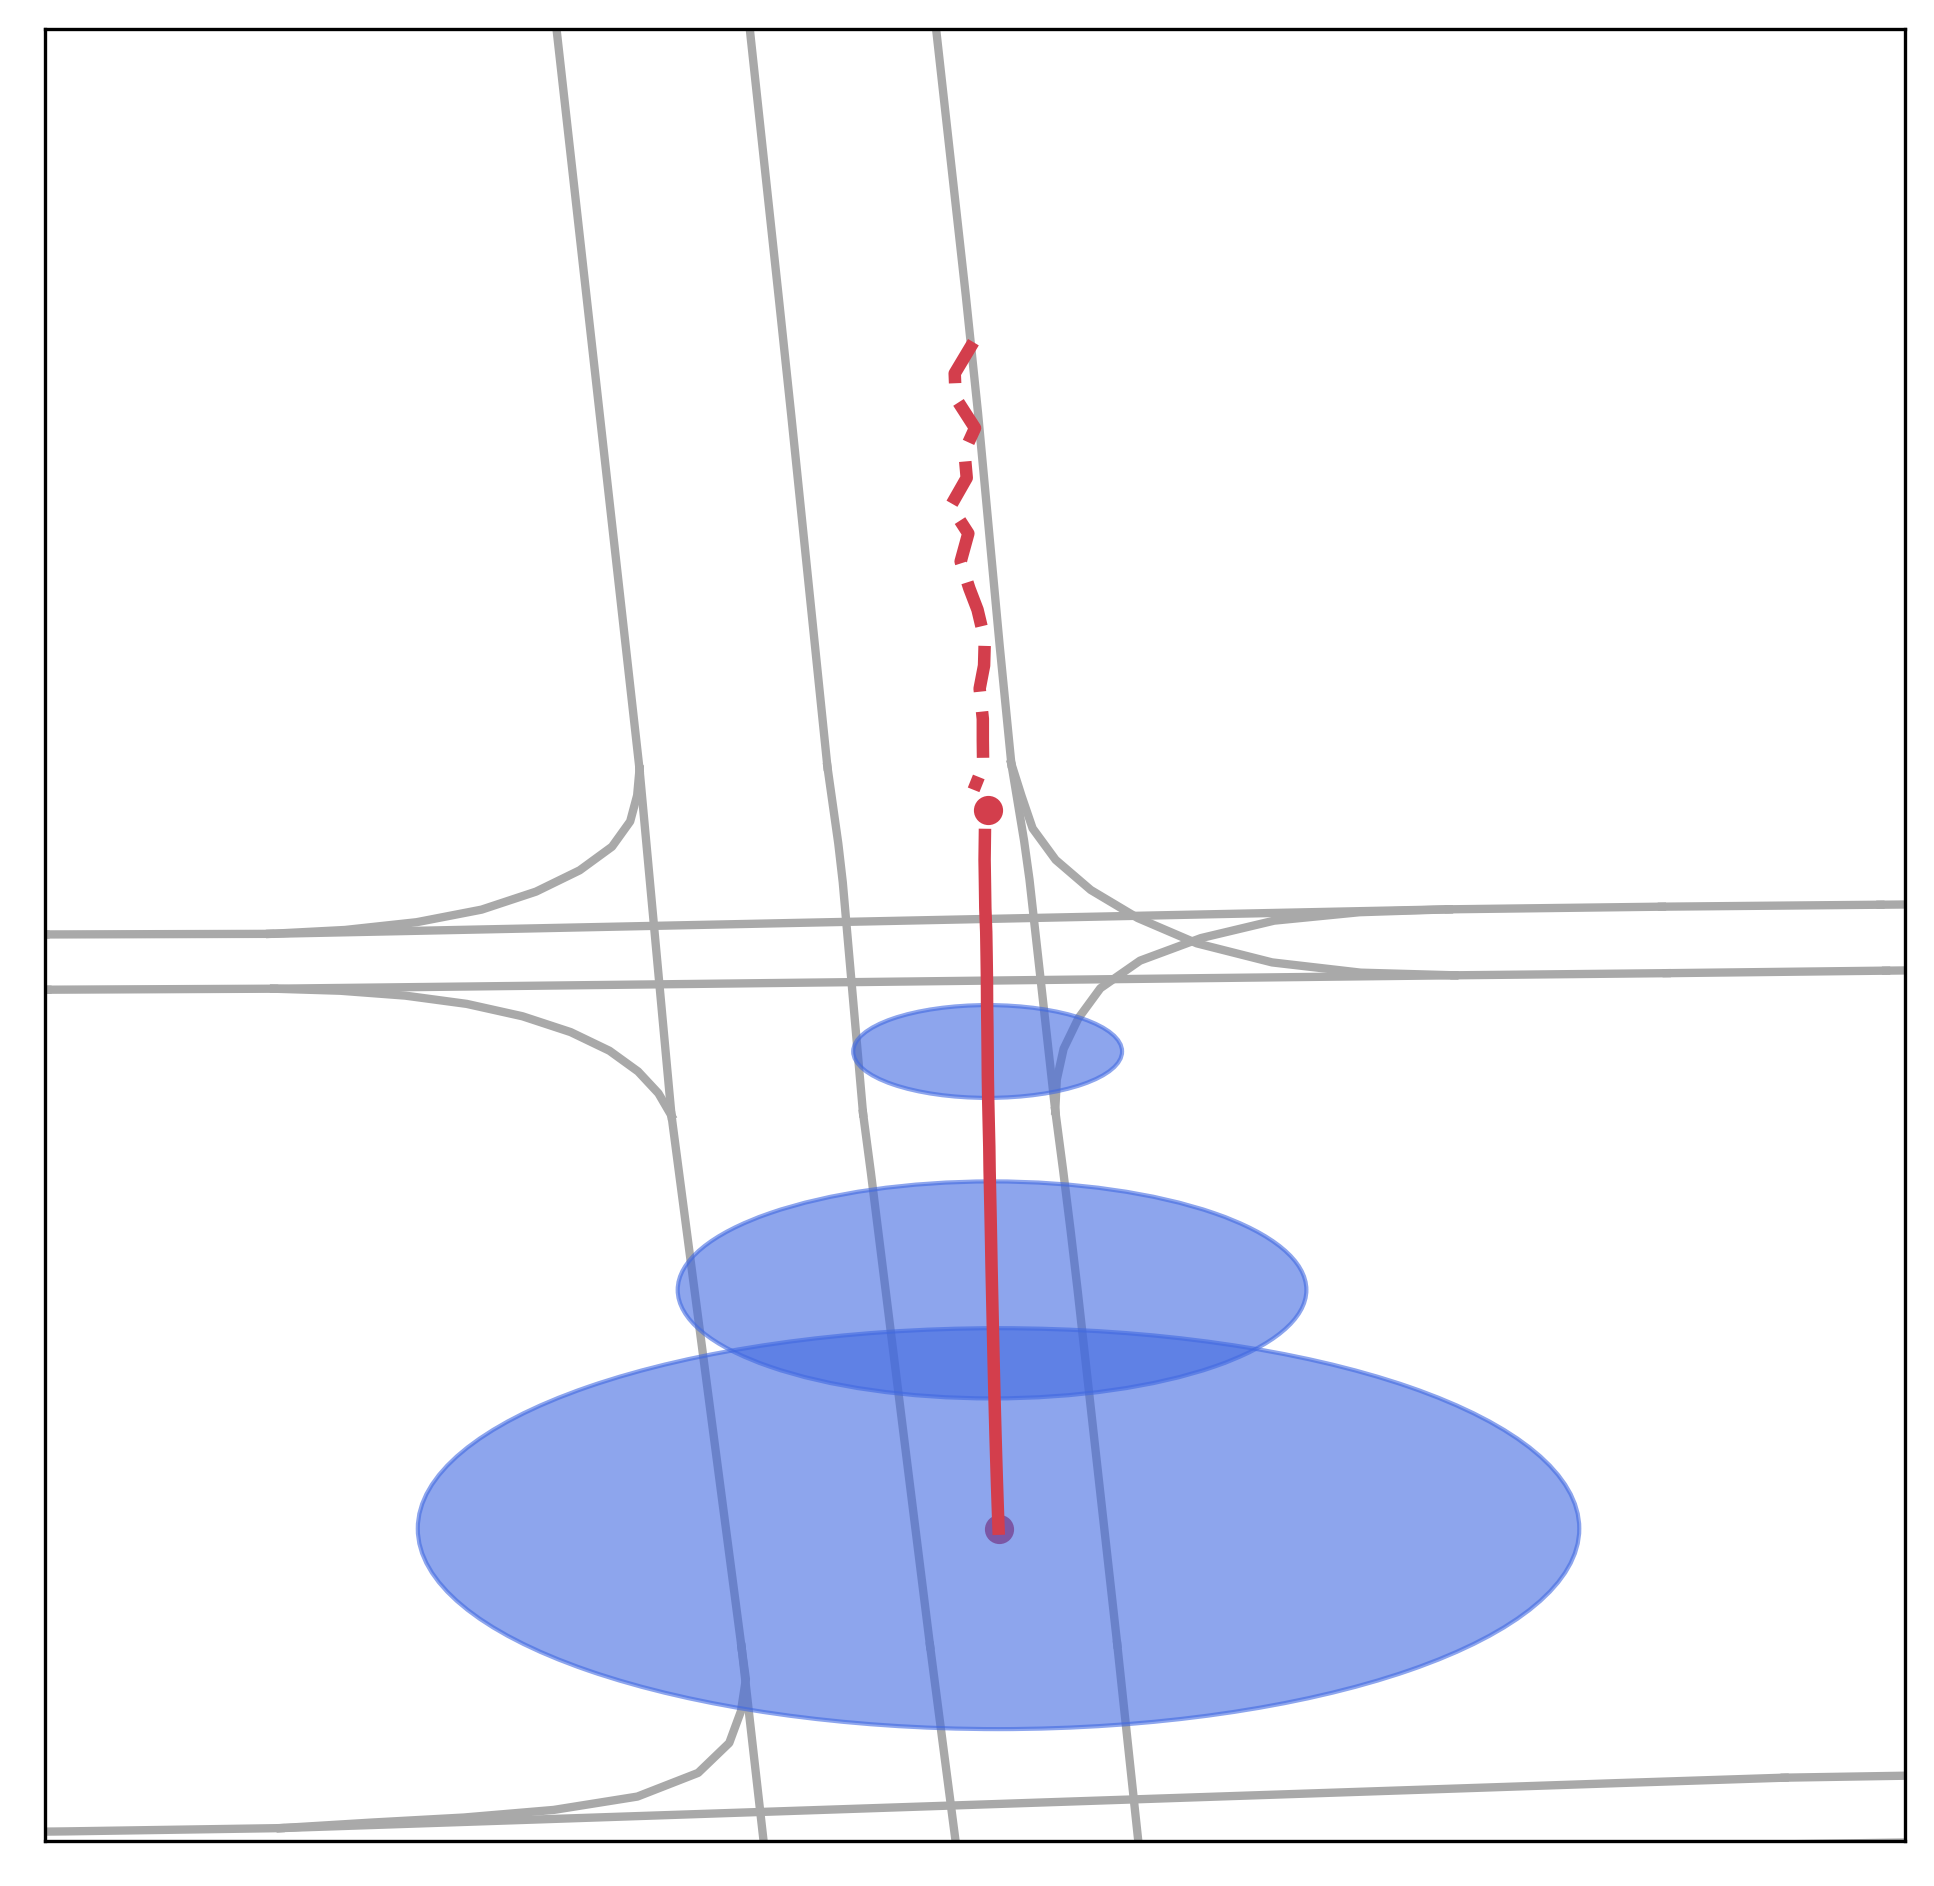
\includegraphics[width=\linewidth]{equivariance/figs/conf1.png}
        \caption{}
    \end{subfigure}%
    \begin{subfigure}[b]{0.245\linewidth}
        \centering
        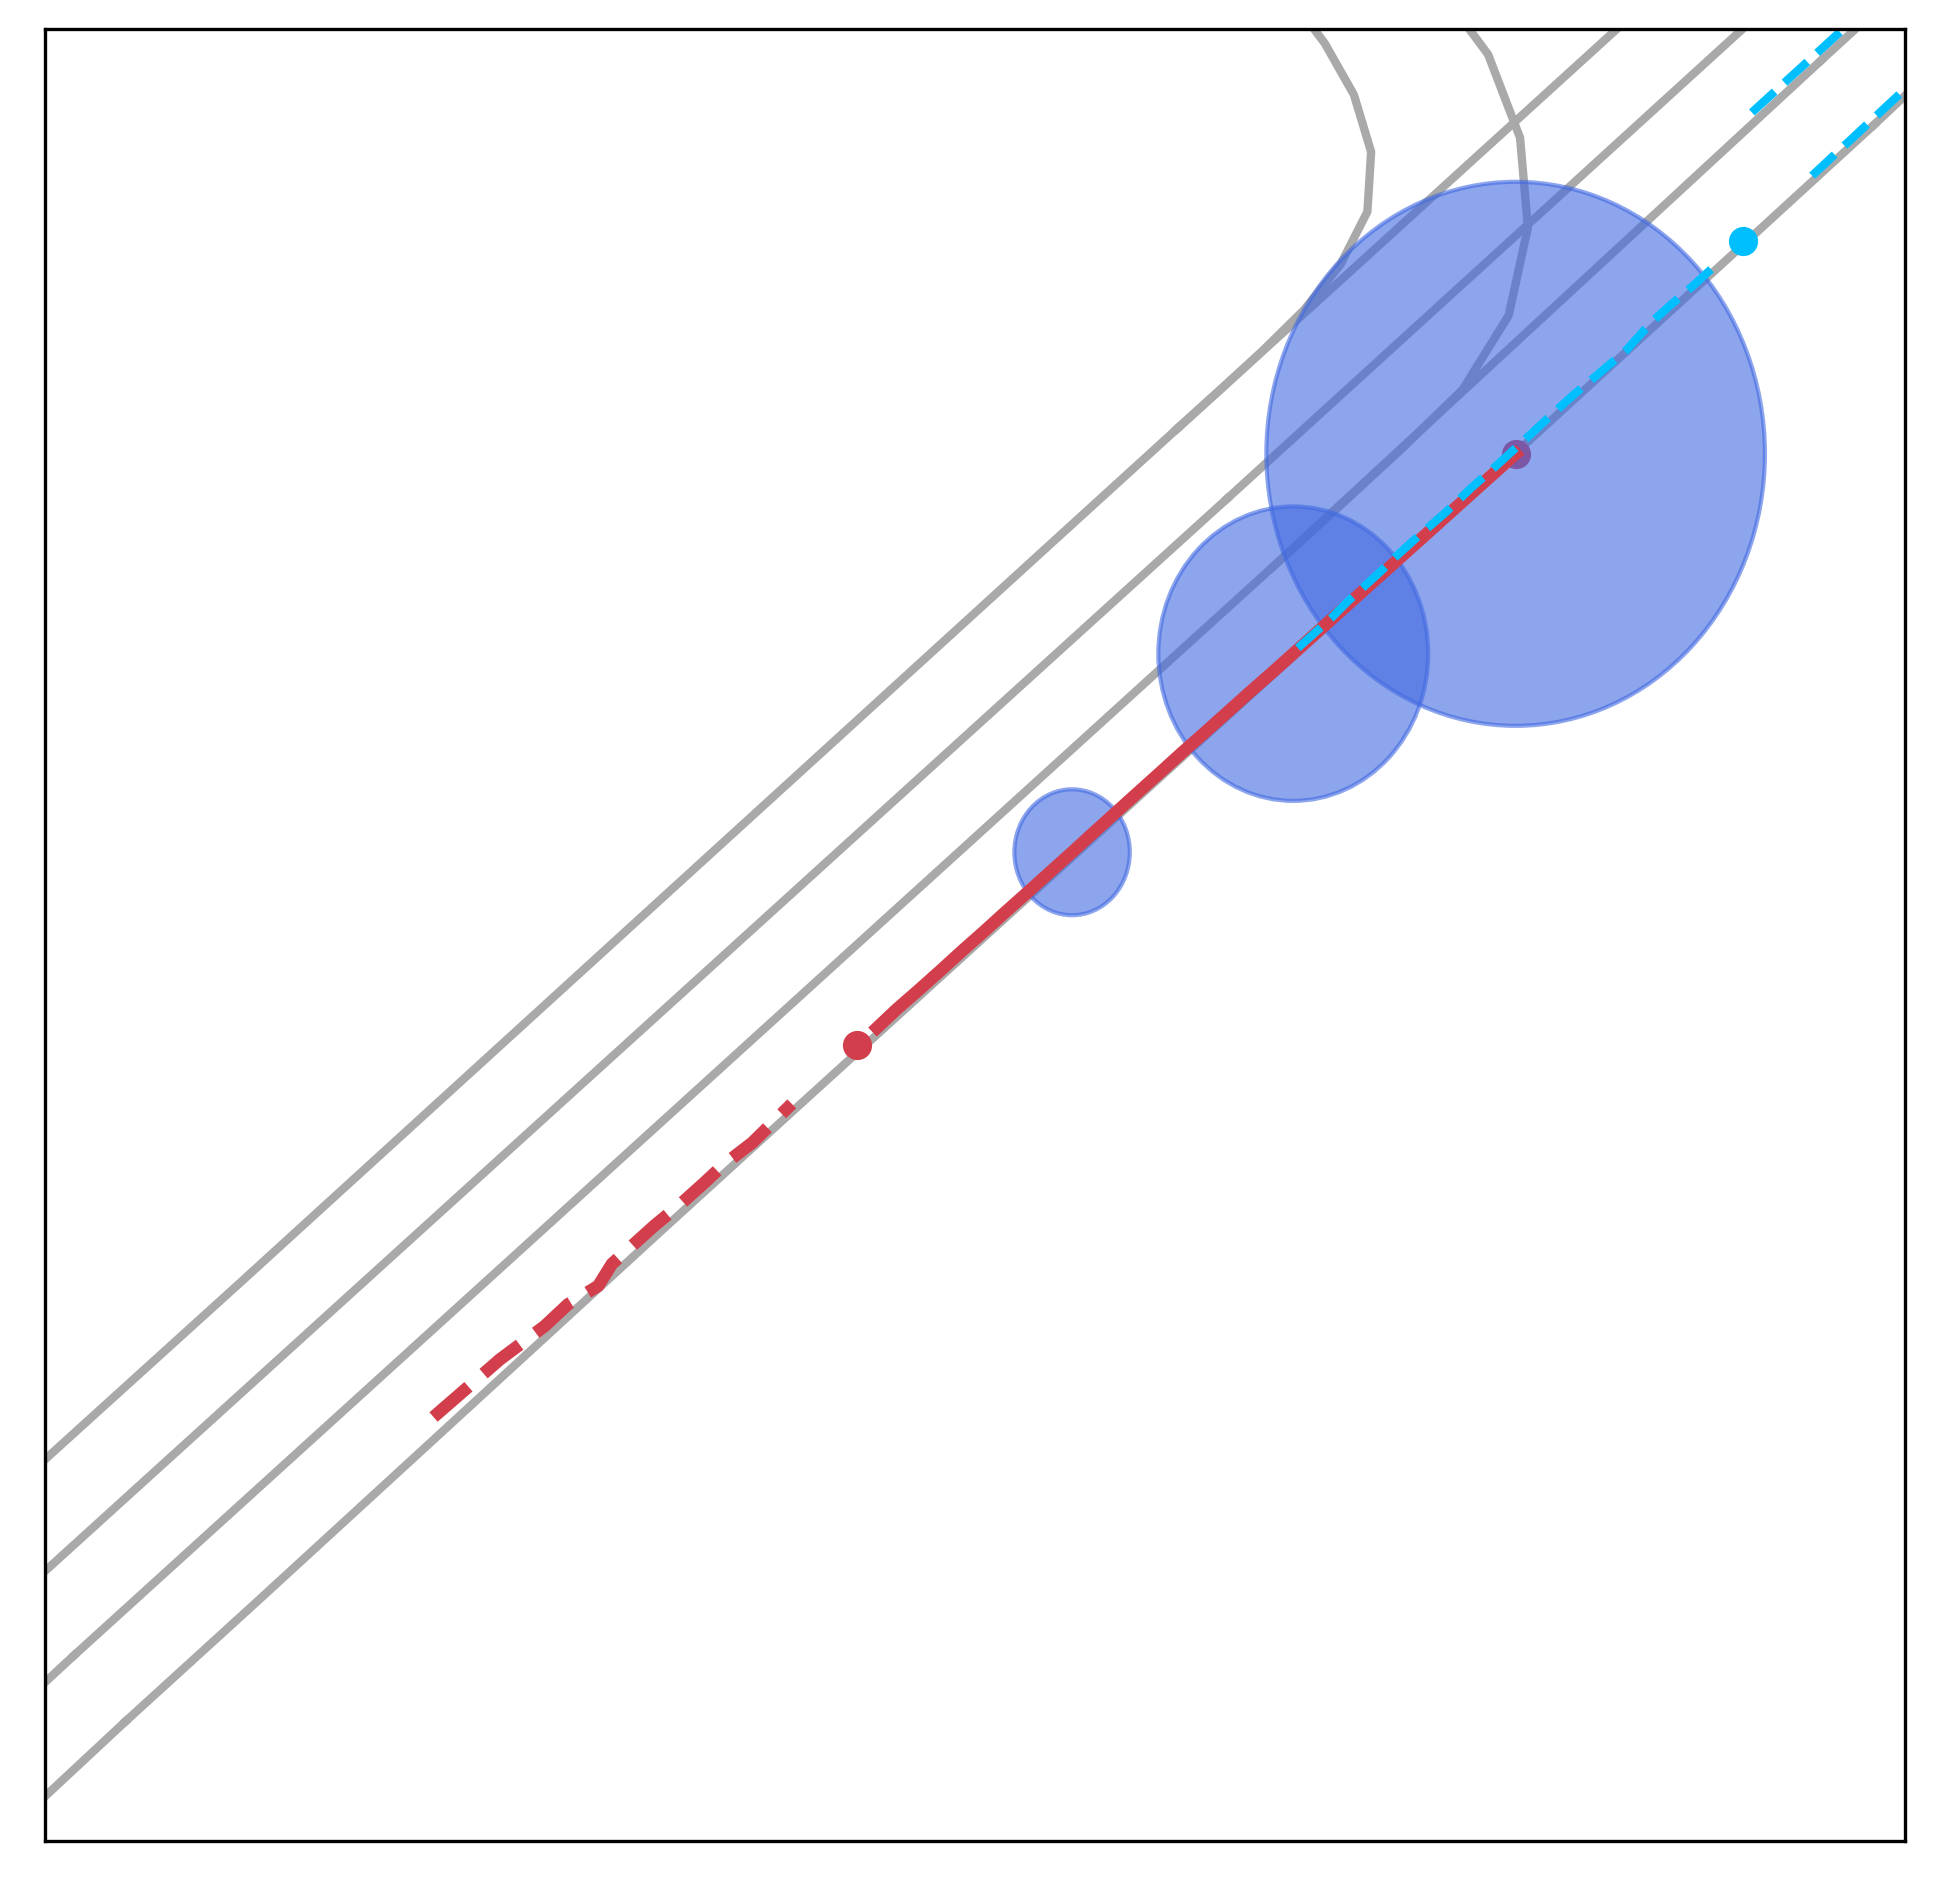
\includegraphics[width=\linewidth]{equivariance/figs/conf2.png}
        \caption{}
    \end{subfigure}%
    \begin{subfigure}[b]{0.245\linewidth}
        \centering
        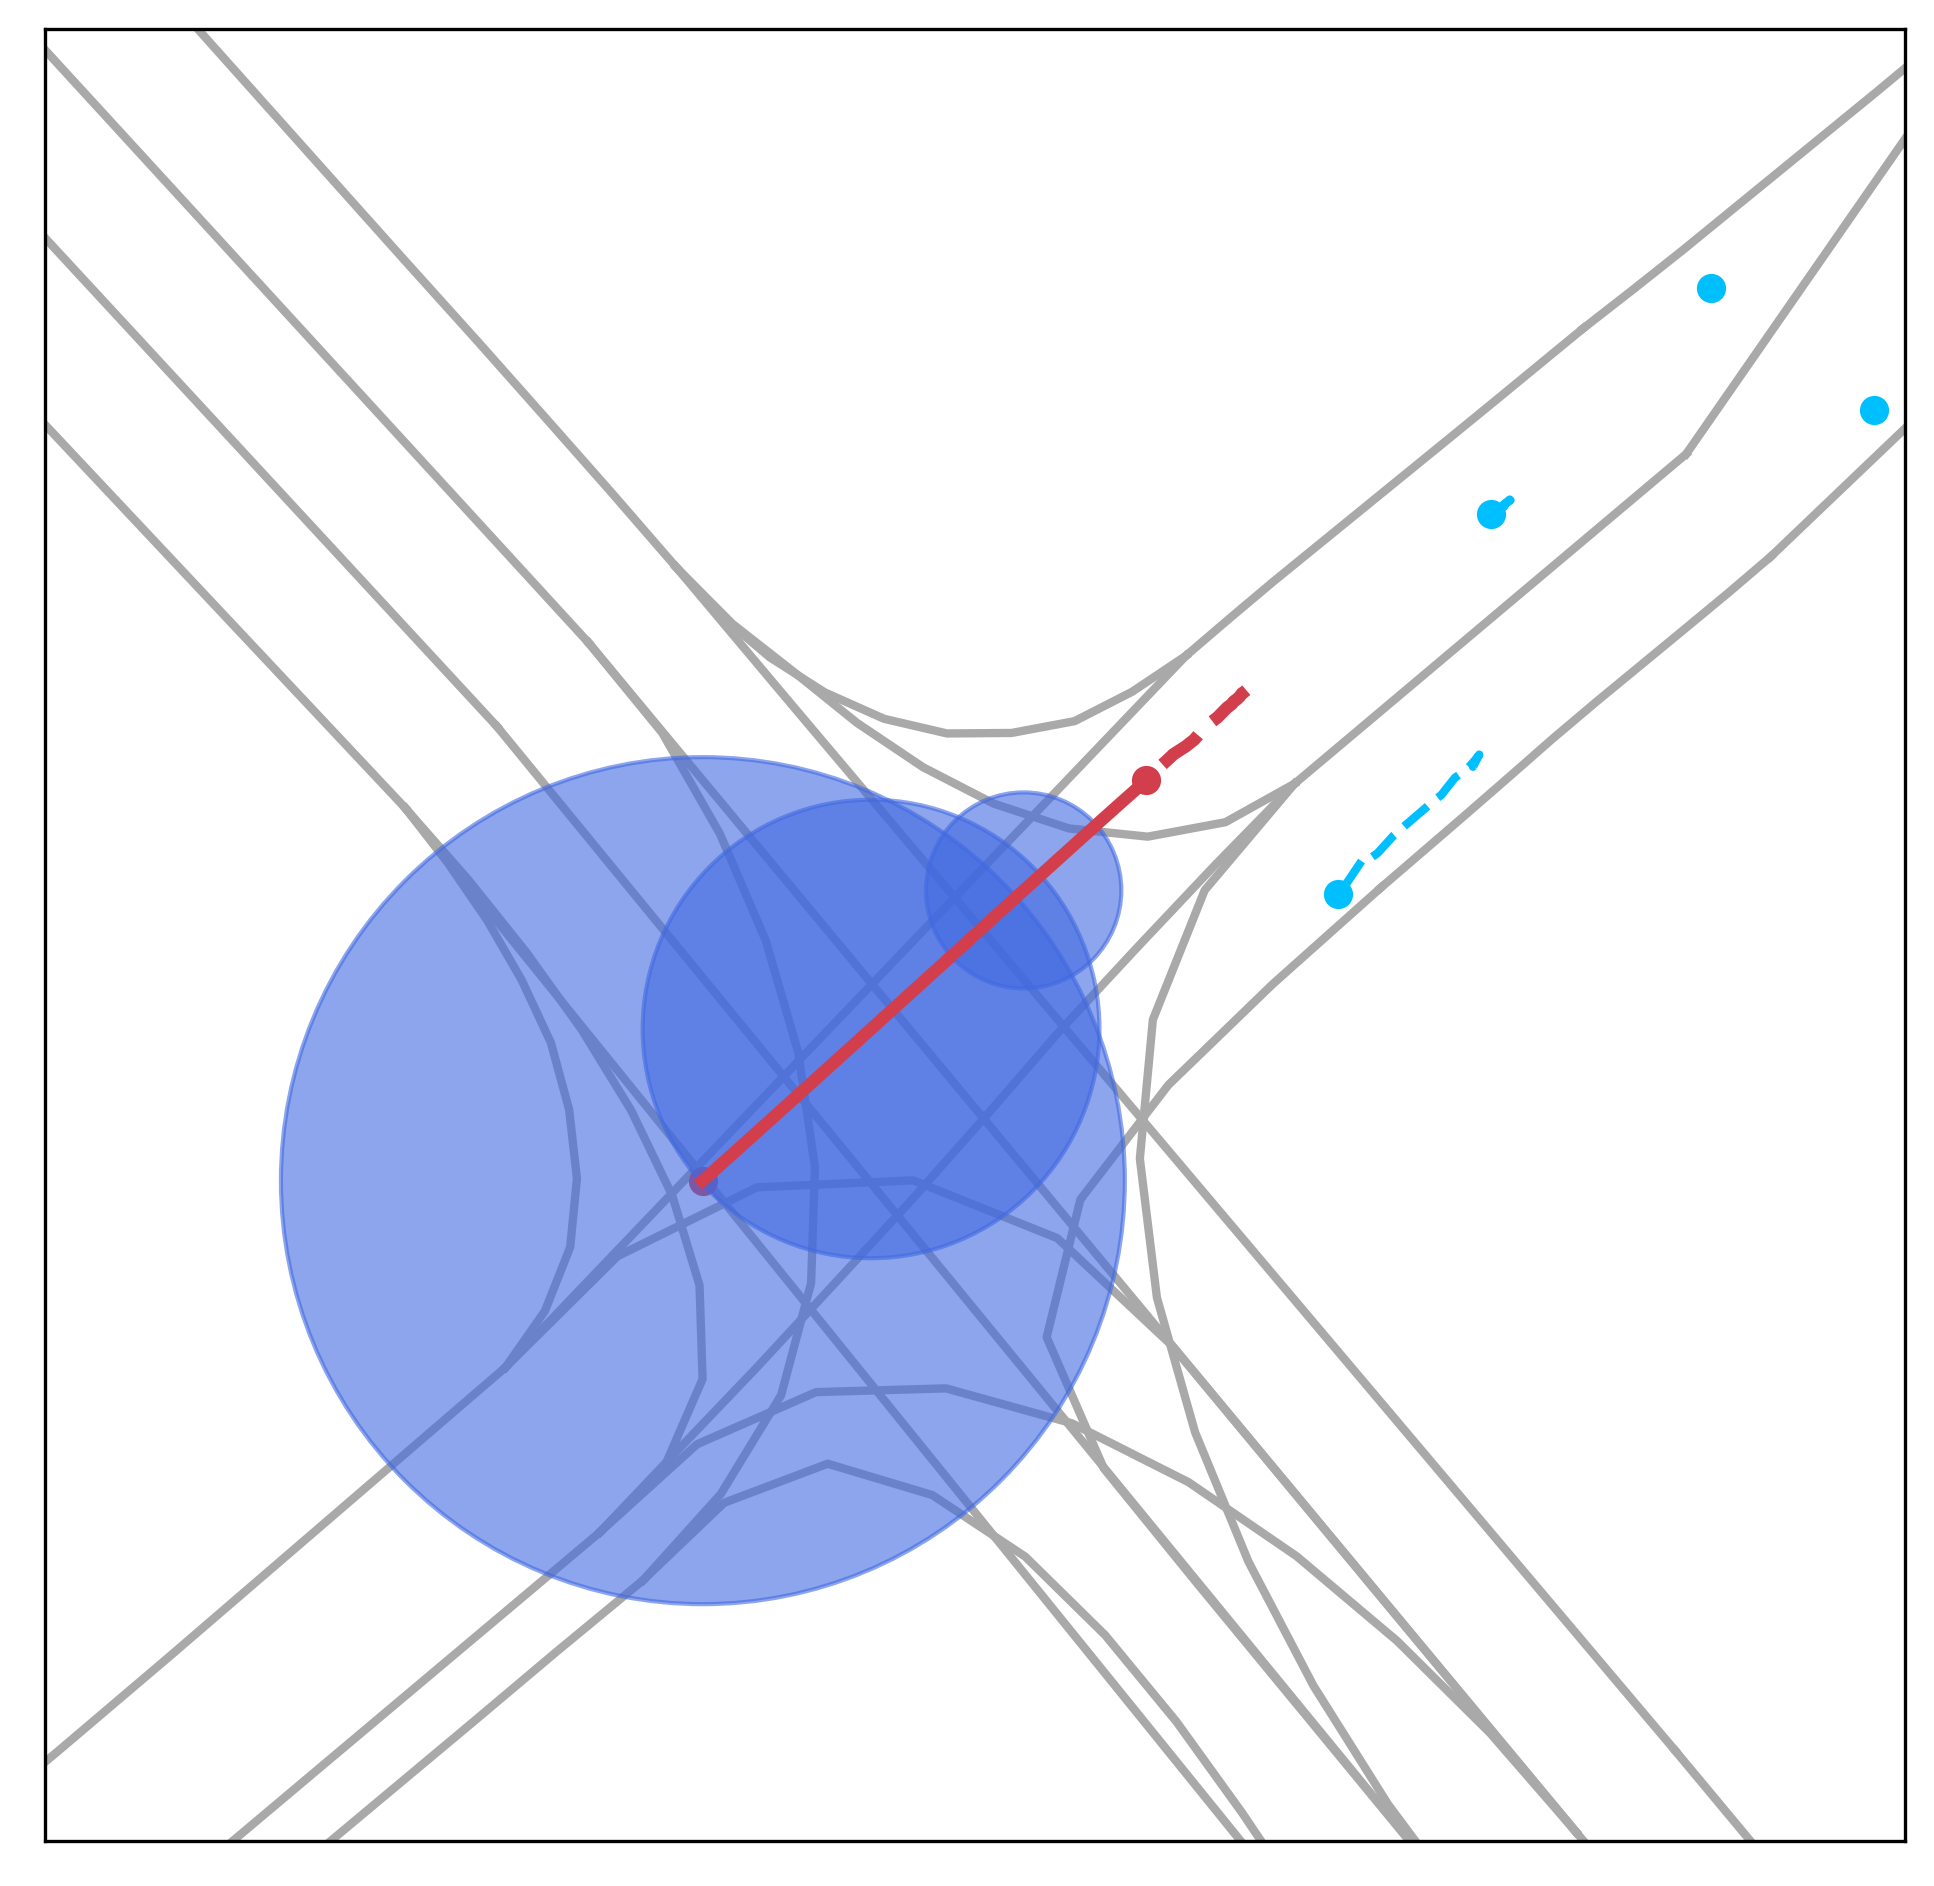
\includegraphics[width=\linewidth]{equivariance/figs/conf3.png}
        \caption{}
        \label{fig:conf3}
    \end{subfigure}%
    \begin{subfigure}[b]{0.245\linewidth}
        \centering
        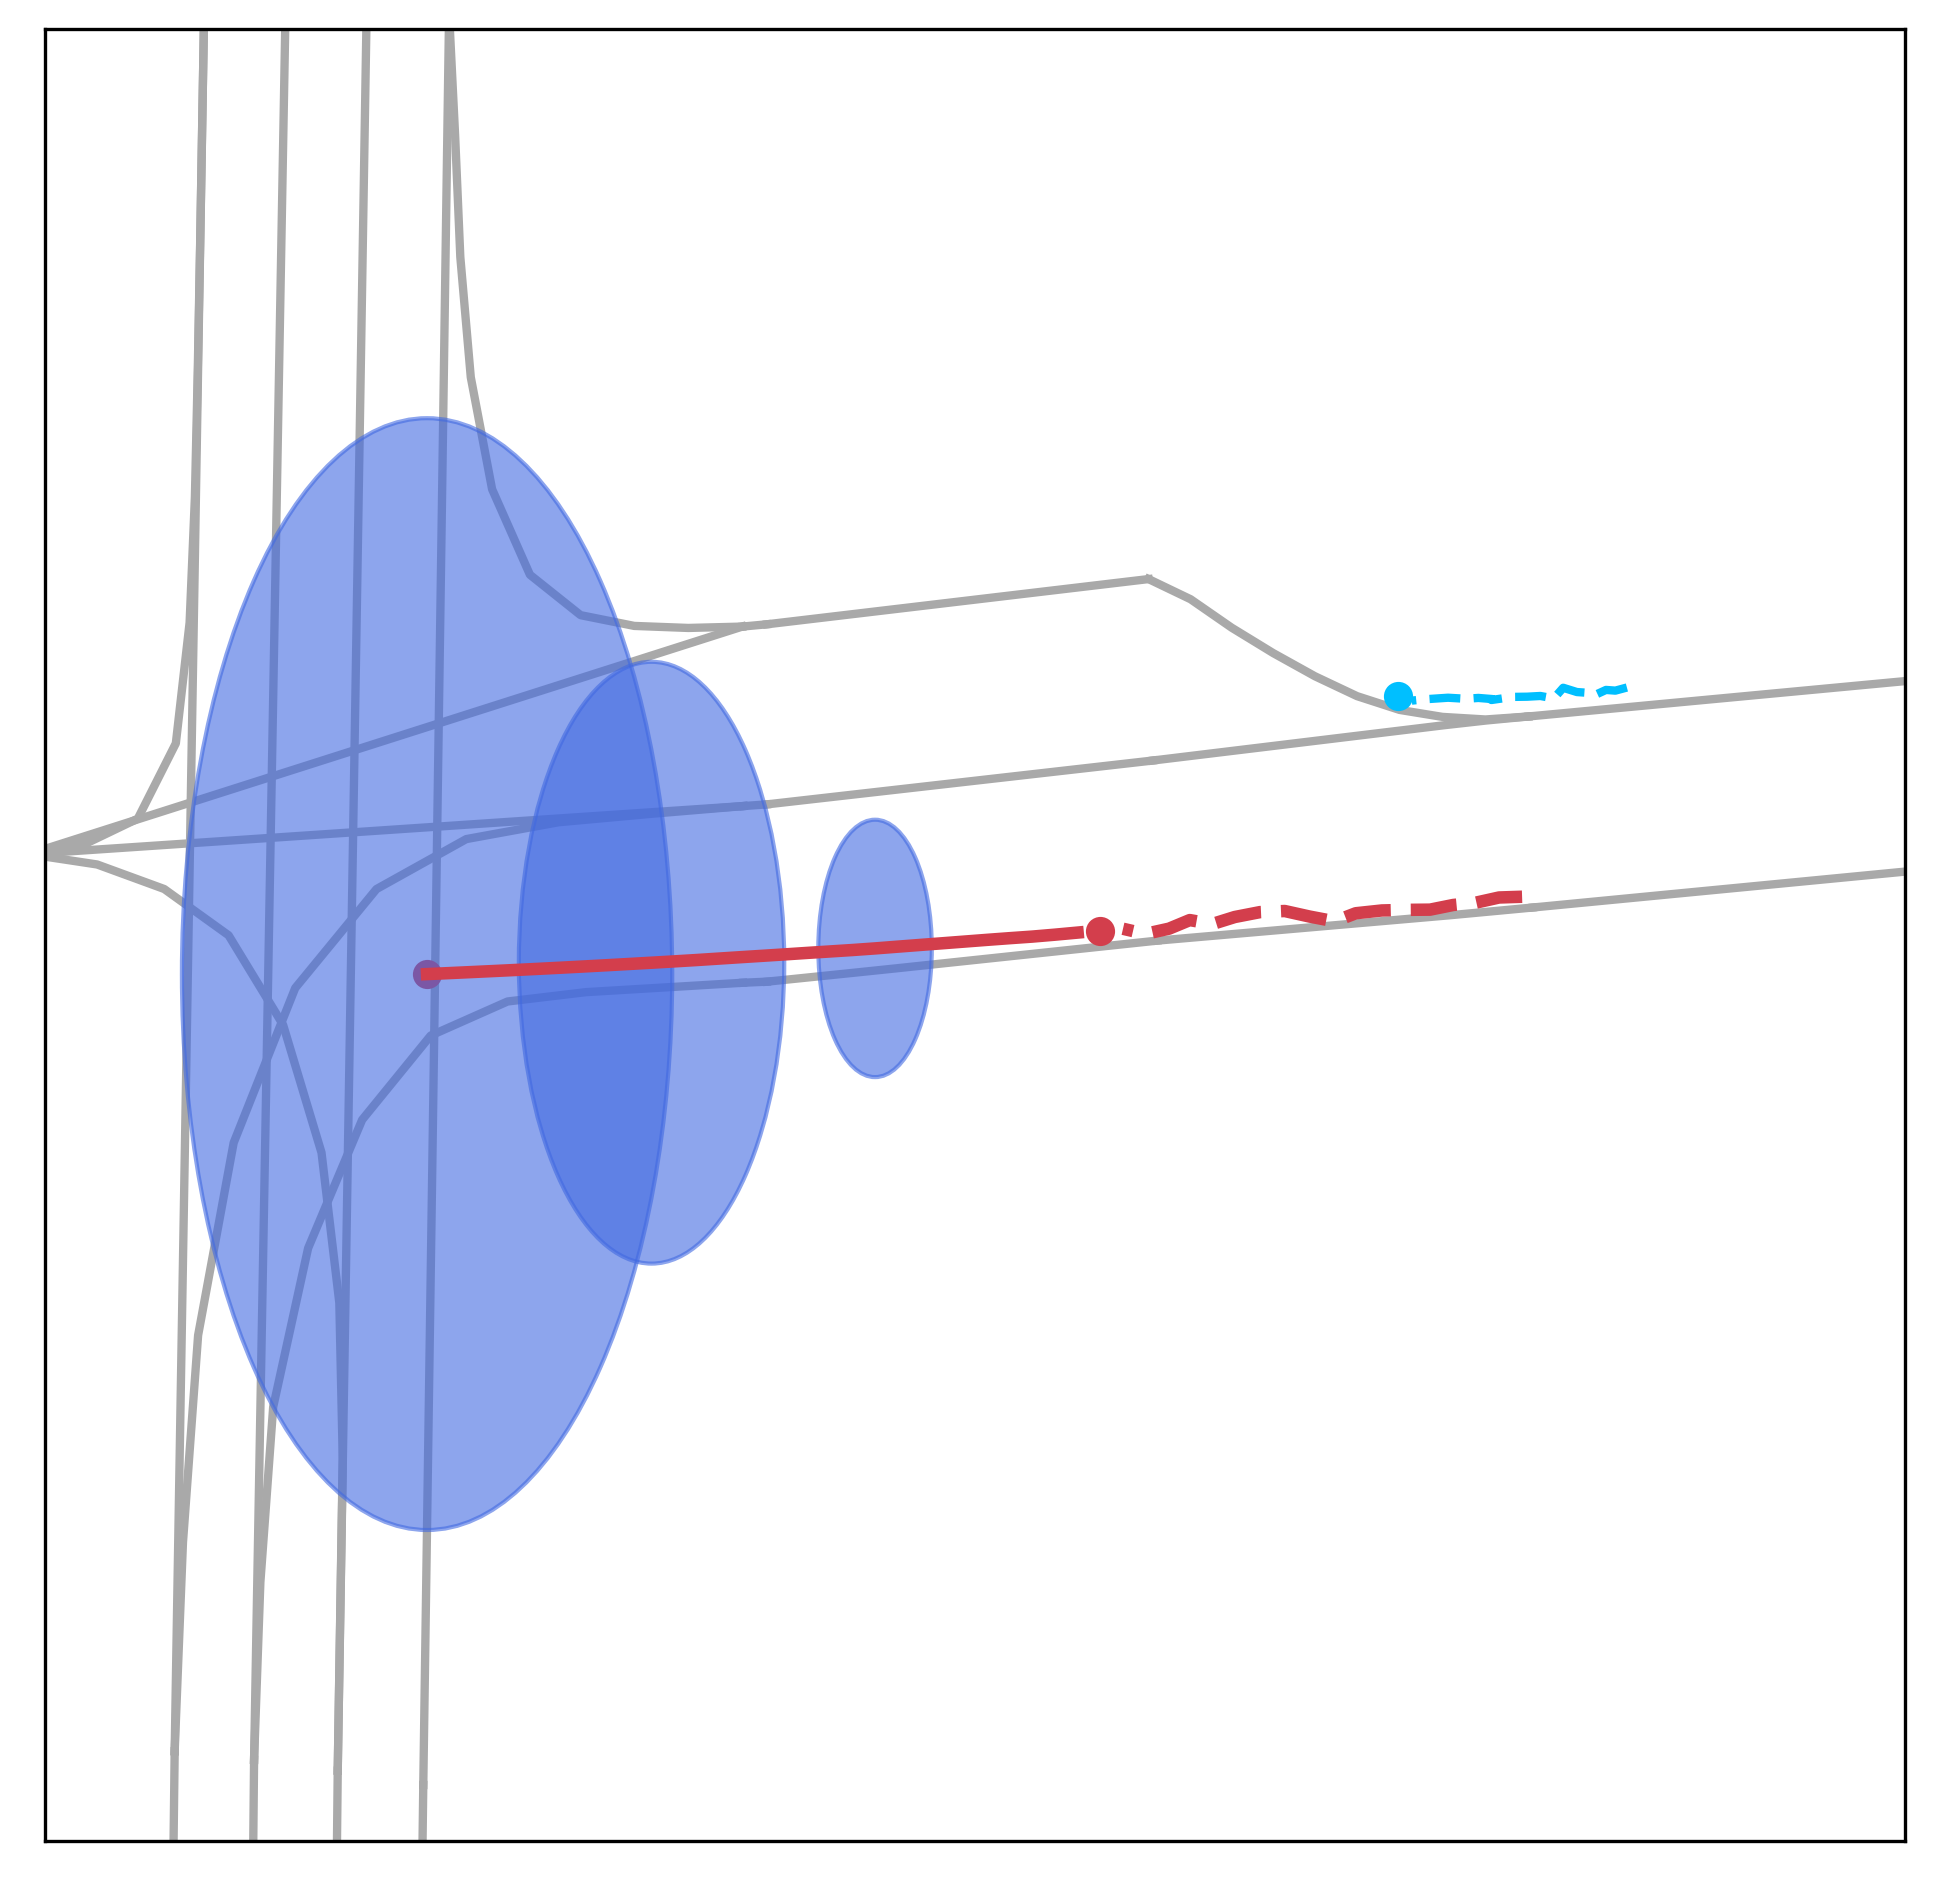
\includegraphics[width=\linewidth]{equivariance/figs/conf7.png}
        \caption{}
        \label{fig:conf7}
    \end{subfigure}
    \caption{Scene illustrations for confidence regions given by conformal-ECCO. Note that in order to achieve 90\% coverage, the region is larger than needed, especially in straight-lane cases like left two scenarios. Due to the lack of underlying assumption about the distribution, the model isn't able to adjust the shape of uncertainty according to data either.}
    \label{fig:conformal}
\end{figure*}


\section{Supplementary: Experiment Details}

\subsection{Implementation Details}
\label{app:exp}

The numbers  in \autoref{tab:big-table} are reported on the official validation set for Argoverse, and on a 10\% test split for TrajNet++. For the particle dataset, the reported numbers are also on a 10\% test split.

\paragraph{Dataset and Preprocessing} 
The synthetic particle dataset is generated by the spring dynamics simulator in \cite{nri}. We added $\sigma=0.01$ noise to the dynamics each step to introduce some uncertainty. The dataset consists of 12,000 time series of trajectories of 5 interacting particles over 50 timesteps ; we use 30 steps as input and predict the following 20 steps. 1,000 samples are used for model validation and 1,000 are used for testing.

The Argoverse autonomous vehicle dataset contains 205,942 samples, consisting of diverse driving scenarios from Miami and Pittsburgh.  We split 90/10 into a training set and validation set of size 185,348 and 20,594 respectively. The official validation set of size 39,472 is used for testing and reporting performance. We preprocess the scenes to filter out incomplete trajectories and cap the number of vehicles modeled to 60. If there are less than 60 cars in the scenario, we insert dummy cars into them to achieve consistent car numbers. For map information, we only include center lanes with lane directions as features. Similar to vehicles, we introduce dummy lane nodes into each scene to make lane numbers consistently equal to 650.

We use the latest release of the TrajNet++ dataset (Update 4.0) for our pedestrian experiments. TrajNet++ is a compiled set of pedestrian trajectories captured in both
indoor and outdoor locations such as in universities, hotels, Zara, and train stations. The sample in this dataset is 21 timestamps long, and the goal is to predict the 2D spatial positions for each pedestrian in the future 12 timestamps given the first 9.
The pedestrian dataset contains 240,896 samples, which we split 80/10/10 into train, validation, and test sets. Similar to Argoverse, we filter out incomplete trajectories in processing and either cap or insert dummy pedestrians such that each scene has 60 agents. No map information was used in the pedestrian dataset. 

We include our code for preprocessing, model implementation, and training in the supplementary materials.

\paragraph{Hyperparameters and Training Details} We trained the PECCO model with 4 equivariant continuous convolution layers of hidden size of (8, 16, 16, 16) respectively for Argoverse, and (4, 8, 16, 16) for the Trajnet++ pedestrian dataset. Our models are all trained with Adam optimizer with a base learning rate $r = 0.001$, and linear learning rate scheduler set to $\gamma = 0.95$.  For Argoverse task, we set the CtsConv radius to be 40, and for the pedestrian task we set it to be 6. PECCO's Arogoverse model has 129k parameters. For comparison, Trajectron++ has 127k and MFP has 67K. 

All our models without map information are trained for 10K iterations with batch size 32 with learning rate updating every 150 iterations. Most of our experiments are performed on a server with 4 RTX 2080 Ti GPUs, and it takes around 9-12 hours to finish training. We run each experiment 3 times with different random initialization and data order. The numbers reported in tables \ref{tab:big-table}, \ref{tab:conformal}, and \ref{tab:deterministic} are the mean and standard deviation of those 3 runs. 

\subsection{Deterministic Baseline Results}
\label{app:deterministic}
We present numbers for deterministic baseline models for Argoverse and Trajnet++. By sampling, we achieve better minADE/minFDE performance with probabilistic models, but they serve as valuable baselines to illustrate the difficulty of the task. 
\begin{table*}[h]
\centering
\begin{tabular}{ c| c c | c c  } 
 \toprule
   &  \multicolumn{2}{c}{Argoverse}  & \multicolumn{2}{c}{Trajnet++}  \\ 
  \midrule
  \textbf{Model}  &  ADE$ \downarrow$ & FDE$\downarrow$ & ADE$ \downarrow$ & FDE$\downarrow$ \\ 
  \midrule
Constant Velocity & 2.77 & 6.16 &1.21 & 2.37\\
Nearest Neighbor   & 3.52 & 7.85 & 1.25 & 2.61\\
LSTM    & 1.97 \plusminus{.05} & 4.98 \plusminus{.31} &1.01  \plusminus{.02}  & 1.98  \plusminus{.08} \\
CtsConv & 1.87 \plusminus{.06} & 4.43 \plusminus{.28} &1.35  \plusminus{.05} & 2.97 \plusminus{.16} \\
ECCO    & 1.68 \plusminus{.04} & 3.98 \plusminus{.19}  & 0.94  \plusminus{.01}  & 2.05 \plusminus{.03} \\
\bottomrule
\end{tabular}
\caption{ Deterministic baselines on the Argoverse and TrajNet++ dataset}
\label{tab:deterministic}
\end{table*}



% \subsection{Visualizations}
% We include 3 more scenarios for qualitatively comparison between models. They provide insights consistent with \autoref{fig:arg-experiment}: LSTM-MRS-r tends to overestimate uncertainty while CtsConv models tend to underestimate collapsing into one mode. PECCO, on the other hand, forecasts a tighter probability that covers the possibilities well.
% \begin{figure*}[ht]
% \centering
% \begin{subfigure}
%   \centering
%   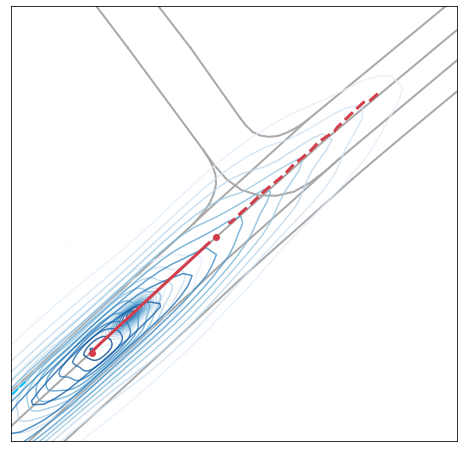
\includegraphics[width=.245\linewidth]{equivariance/figs/10011lstm.png}
%   \caption{LSTM-MRS-r}
%   \label{fig:sub1}
% \end{subfigure}%
% \begin{subfigure}
%   \centering
%   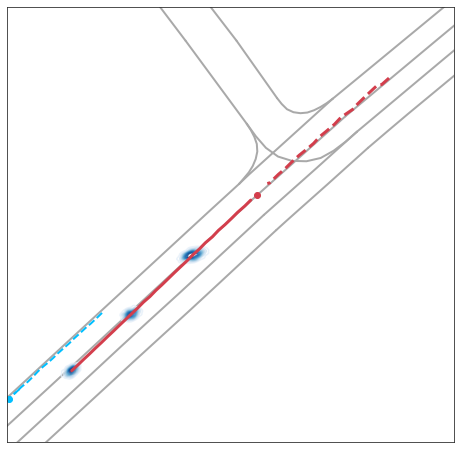
\includegraphics[width=.245\linewidth]{equivariance/figs/10011nll.png}
%   \caption{CtsConv-NLL}
%   \label{fig:sub2}
% \end{subfigure}
% \begin{subfigure}
%   \centering
%   \includegraphics[width=.245\linewidth]{equivariance/figs/10011mis.png}
%   \caption{CtsConv-MRS}
%   \label{fig:sub3}
% \end{subfigure}%
% \begin{subfigure}
%   \centering
%   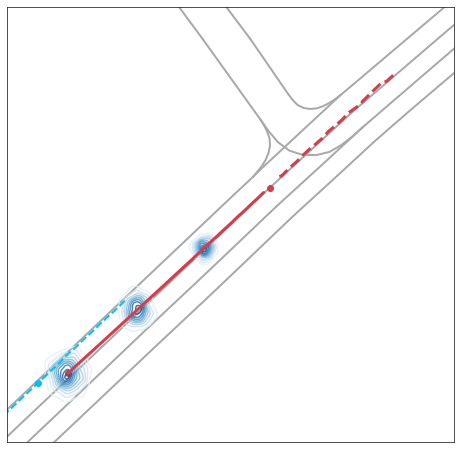
\includegraphics[width=.24\linewidth]{equivariance/figs/10011dyna.png}
%   \caption{PECCO}
%   \label{fig:sub4}
% \end{subfigure}
% \caption{Another lane change example. Red trajectories is the agent of interest in the same scenario. CtsConv-NLL and CtsConv-MRS captured two different modes of futures, whereas PECCO is able to cover both.}
% \label{fig:arg-experiment-2}
% \end{figure*}



% \begin{figure*}[ht]
% \centering
% \begin{minipage}{0.245\textwidth}
%   \centering
%   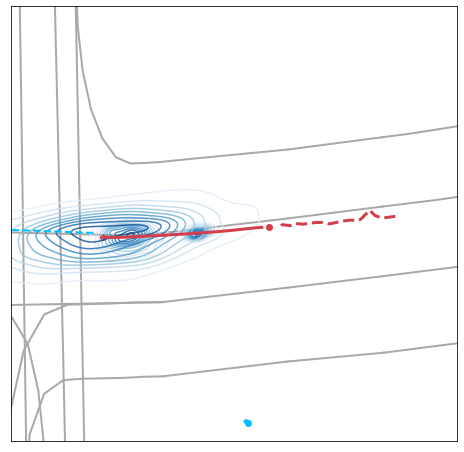
\includegraphics[width=.9\linewidth]{equivariance/figs/10057lstm.png}
%   \subcaption{LSTM-MRS-r}
%   \label{fig:sub1}
% \end{minipage}%
% \begin{minipage}{0.245\textwidth}
%   \centering
%   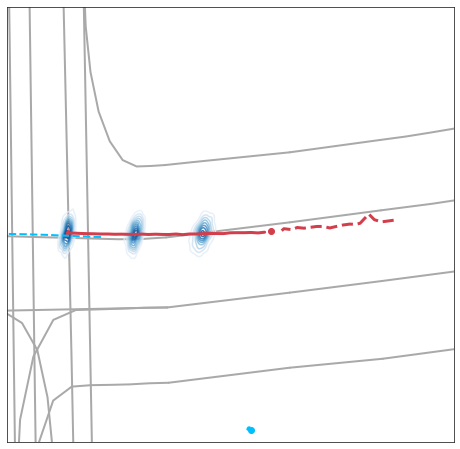
\includegraphics[width=.9\linewidth]{equivariance/figs/10057nll.png}
%   \subcaption{CtsCov-NLL}
%   \label{fig:sub2}
% \end{minipage}%
% \begin{minipage}{0.245\textwidth}
%   \centering
%   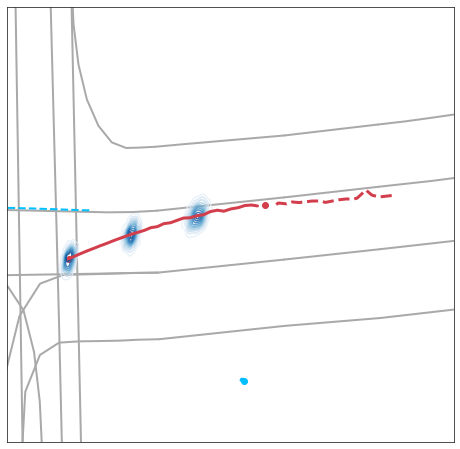
\includegraphics[width=.9\linewidth]{equivariance/figs/10057mis.png}
%   \subcaption{CtsConv-MRS}
%   \label{fig:sub3}
% \end{minipage}%
% \begin{subfigure}
%   \centering
%   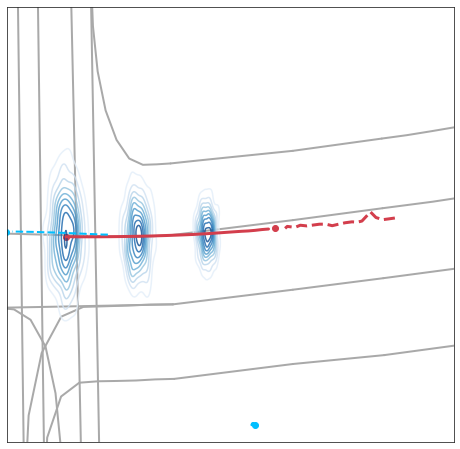
\includegraphics[width=.23\linewidth]{equivariance/figs/10057dyna.png}
%   \caption{PECCO}
%   \label{fig:sub4}
% \end{subfigure}\\
% \begin{subfigure}
%   \centering
%   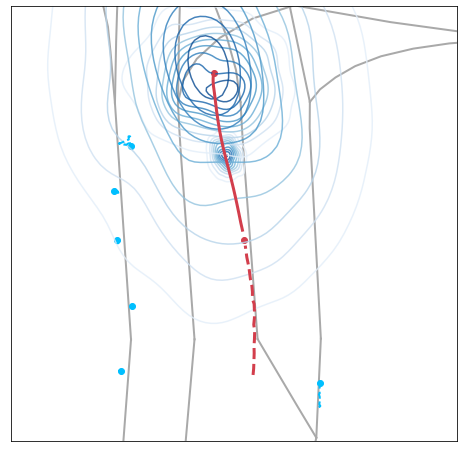
\includegraphics[width=.23\linewidth]{equivariance/figs/10003lstm.png}
%   \caption{LSTM-MRS-r}
%   \label{fig:sub1}
% \end{subfigure}%
% \begin{subfigure}
%   \centering
%   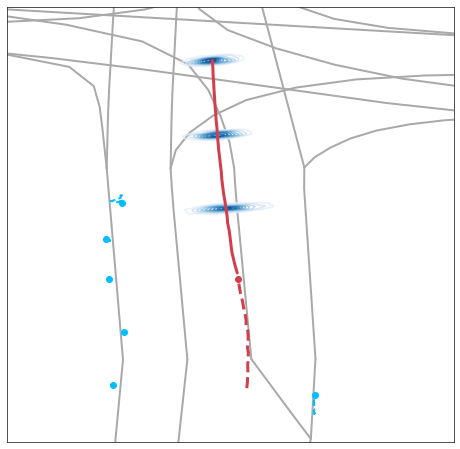
\includegraphics[width=.23\linewidth]{equivariance/figs/10003nll.png}
%   \caption{CtsConv-NLL}
%   \label{fig:sub2}
% \end{subfigure}
% \begin{subfigure}
%   \centering
%   \includegraphics[width=.23\linewidth]{equivariance/figs/10003mis.png}
%   \caption{CtsConv-MRS}
%   \label{fig:sub3}
% \end{subfigure}%
% \begin{subfigure}
%   \centering
%   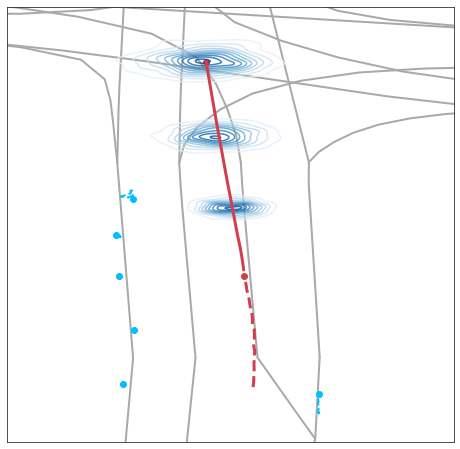
\includegraphics[width=.23\linewidth]{equivariance/figs/10003dyna.png}
%   \caption{PECCO}
%   \label{fig:sub4}
% \end{subfigure}
% \caption{Comparison of uncertainty predicted at 2 crossroads. Red trajectories is the agent of interest in the same scenario. Note how the LSTM predicted uncertainty explodes at the final time step, and PECCO is able to model the possibility of turns. }
% \label{fig:arg-experiment-1}
% \end{figure*}




% %-- archive--

% \begin{figure*}[ht]
% \centering
% \begin{subfigure}
%   \centering
%   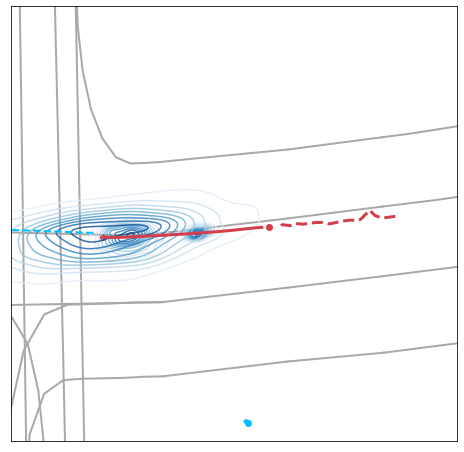
\includegraphics[width=.23\linewidth]{equivariance/figs/10057lstm.png}
%   \caption{LSTM-MRS-r}
%   \label{fig:sub1}
% \end{subfigure}%
% \begin{subfigure}
%   \centering
%   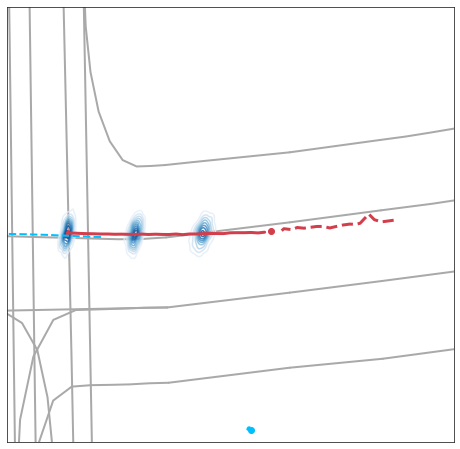
\includegraphics[width=.23\linewidth]{equivariance/figs/10057nll.png}
%   \subcaption{CtsCov-NLL}
%   \label{fig:sub2}
% \end{subfigure}
% \begin{subfigure}
%   \centering
%   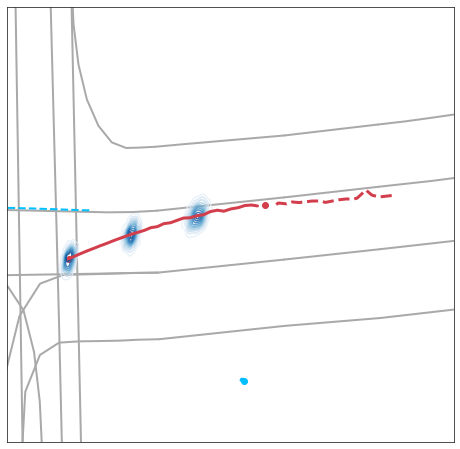
\includegraphics[width=.23\linewidth]{equivariance/figs/10057mis.png}
%   \caption{CtsConv-MRS}
%   \label{fig:sub3}
% \end{subfigure}%
% \begin{subfigure}
%   \centering
%   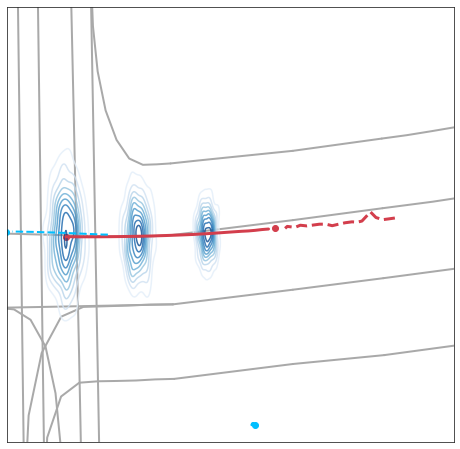
\includegraphics[width=.23\linewidth]{equivariance/figs/10057dyna.png}
%   \caption{PECCO}
%   \label{fig:sub4}
% \end{subfigure}\\
% \begin{subfigure}
%   \centering
%   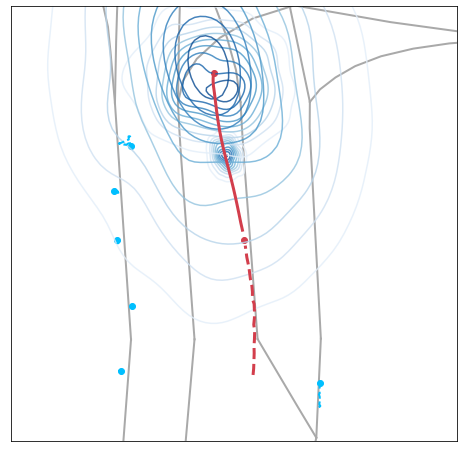
\includegraphics[width=.23\linewidth]{equivariance/figs/10003lstm.png}
%   \caption{LSTM-MRS-r}
%   \label{fig:sub1}
% \end{subfigure}%
% \begin{subfigure}
%   \centering
%   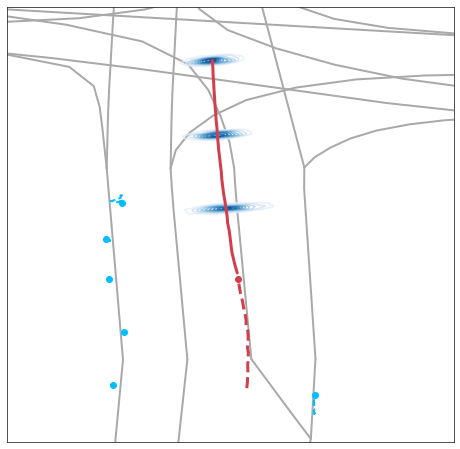
\includegraphics[width=.23\linewidth]{equivariance/figs/10003nll.png}
%   \caption{CtsConv-NLL}
%   \label{fig:sub2}
% \end{subfigure}
% \begin{subfigure}
%   \centering
%   \includegraphics[width=.23\linewidth]{equivariance/figs/10003mis.png}
%   \caption{CtsConv-MRS}
%   \label{fig:sub3}
% \end{subfigure}%
% \begin{subfigure}
%   \centering
%   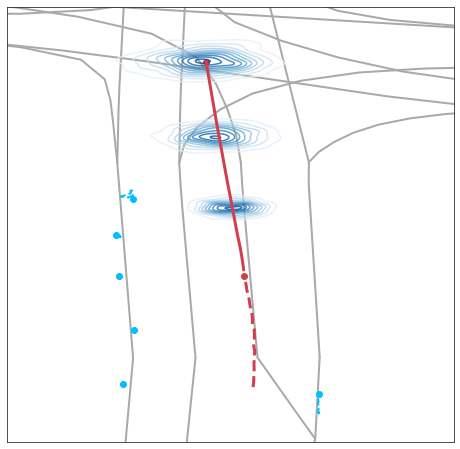
\includegraphics[width=.23\linewidth]{equivariance/figs/10003dyna.png}
%   \caption{PECCO}
%   \label{fig:sub4}
% \end{subfigure}
% \caption{Comparison of uncertainty predicted at 2 crossroads. Red trajectories is the agent of interest in the same scenario. Note how the LSTM predicted uncertainty explodes at the final time step, and PECCO is able to model the possibility of turns. }
% \label{fig:arg-experiment-1}
% \end{figure*}




%\textbf{Model Parameters and Data Efficiency.}
%A major benefit of incorporating the inductive bias of equivariance is to improve the sample efficiency of learning, as equivariance collapses the domain space by a factor of the size of the symmetry group \cite{wang2020incorporating}. Thus PECCO requires far fewer samples to learn from.




\chapter{Copula Conformal prediction for multi-step time series prediction}

% \begin{abstract}
% Accurate uncertainty measurement is a key step to building robust and reliable machine learning systems. Conformal prediction is a distribution-free uncertainty quantification algorithm popular for its ease of implementation, statistical coverage guarantees, and versatility for underlying forecasters. However, existing conformal prediction algorithms for time series are limited to single-step prediction without considering the temporal dependency. In this paper we propose a \textbf{Copula} \textbf{C}onformal \textbf{P}rediction algorithm for multivariate, multi-step \textbf{T}ime \textbf{S}eries forecasting, \textbf{CopulaCPTS}. On several synthetic and real-world multivariate  time series datasets,  we show that CopulaCPTS produces more calibrated and sharp confidence intervals for multi-step prediction tasks than existing techniques. 
% \end{abstract}

\section{Introduction}
Deep learning  models are becoming widely used in high-risk settings such as healthcare, transportation, and finance. In these settings, it is important that a model produces calibrated uncertainty to reflect its own confidence and to assist decision making. Confidence regions are a common approach to quantify forecast uncertainty \cite{khosravi2011comprehensive}. A $(1-\alpha)$-confidence region $\Gamma^{1-\alpha}$ for a random variable $y$ is \textit{valid} if it contains $y$'s true value with high probability:  $\Prob(y \in \Gamma^{1-\alpha}) \geq 1-\alpha$. Note one can make  $\Gamma^{1-\alpha}$ infinitely wide to satisfy validity. For the confidence region to be useful, we want to minimize its area while remaining valid; this is known as the \textit{efficiency} of the region. 

Conformal prediction is a powerful method that produces confidence regions with finite-sample guarantees of validity  \cite{vovk2005algorithmic, lei2018distribution}. Furthermore, it makes no assumptions about the forecast model or the underlying data distribution. Its generality, simplicity, and statistical guarantees have made conformal prediction popular for many real world applications including drug discovery \cite{eklund2015application} and robotics \cite{luo2021sample}.

In this paper we present a more calibrated and efficient conformal prediction algorithm for multi-step times series forecasting. This type of problem is ubiquitous - examples include predicting hurricane paths, vehicle trajectories, and financial or epidemic forecasts. To quantify uncertainty, we want a "cone of uncertainty" that covers the entirety of the forecast horizon. \cite{Schaar2021conformaltime} presented an algorithm, CF-RNN, for multi-step time series with the assumption that all time steps are modeled independently. In practice, however, we found that CF-RNN produces confidence regions often too large to be useful, especially when the problem is multivariate or has a long forecast horizon. 

% 1. widely used in economics
% 2. Machine learning for probablisitic time series forecasting, but not related to CP
% 3. There is one work in the CP literature use copula to model dependencies between multiple targets (non temporal) by messoudi et al.

We introduce  \textbf{CopulaCPTS}, a \textbf{Copula}-based \textbf{C}onformal \textbf{P}rediction algorithm for multi-step \textbf{T}ime \textbf{S}eries forecasting. We improve efficiency by utilizing copulas to model the dependency between forecasted time steps. 
A copula is a multivariate cumulative distribution function that models the dependence between multiple random variables. It is widely used in economic forecasting \cite{nelsen2007introduction, patton2012review} and has been introduced to conformal algorithms by \cite{messoudi2021copula} to model correlation between multiple targets in non-temporal settings. Copula processes have been explored in generative models for time series \cite{salinas2019high, drouin2022tactis}. We found that copulas are effective in capturing uncertainty relations between time steps. Our contributions are: 
\begin{itemize}
    \item \textbf{CopulaCPTS} is a general uncertainty quantification algorithm that can be applied to \textit{any} multivariate  multi-step forecaster, with statistical guarantees of validity.
    \item \textbf{CopulaCPTS} produces significantly sharper and more calibrated uncertainty estimates than state-of-the-art baselines on 4 benchmark datasets, both synthetic and real.
    \item We present a re-calibration technique such that \textbf{CopulaCPTS} can produce valid confidence intervals for time series forecasts of varying lengths. 
\end{itemize}

% and is explored in the ML multi-variate time series literature \cite{salinas2019high, drouin2022tactis}. 

% Conformal prediction (CP) is a method for evaluating uncertainty for machine learning predictions and producing prediction sets (for classification) or confidence intervals (for regression) in a distribution-free manner. Conformal prediction, originally introduced by \cite{vovk2005algorithmic}, provides a framework to quantify prediction uncertainty and generate confidence regions without making any assumptions on the data distribution. It has gained popularity because of its finite-sample coverage guarantees and implementation simplicity. Many has worked on extending CP to different tasks and prediction algorithms, such as for the inductive setting \cite{vovk2005algorithmic}, multi-label classification \cite{wang2015comparison}, and multi-target regression \cite{messoudi2020multitarget}. 

\section{Related Work}

\paragraph{Uncertainty Quantification for Deep Time-Series Forecasting} The two major paradigms of  Uncertainty Quantification (UQ) methods for deep neural networks are Bayesian and Frequentist. Bayesian approaches estimate a distribution over the model parameters given data, and then marginalize these parameters to form output distributions via Markov Chain Monte Carlo (MCMC) sampling \cite{welling2011bayesian, neal2012bayesian, chen2014stochastic} or variational inference (VI)  \cite{graves2011practical,kingma2015variational, blundell2015weight, louizos2017multiplicative}. \cite{wang2019deep, wu2021quantifying} propose Bayesian Neural Network (BNN)-based models for UQ of spatiotemporal forecasts. In practice, Bayesian UQ has two major drawbacks: (1) it requires significant modification to the training process of deep models, and (2) BNNs can be computationally expensive and difficult to optimize, especially for larger networks \cite{lakshminarayanan2017simple, zadrozny2001obtaining}. UQ for deep neural network time series forecasts often adopt approximate Bayesian inference such as MC-dropout \cite{gal2016theoretically, gal2017concrete}.

Frequentist UQ methods emphasize robustness against variations in the data. These approaches either rely on resampling the data or learning an interval bound to encompass the dataset. For time series forecasting UQ, frequentist approaches include ensemble methods such as bootstrap \cite{efron2016, alaa2020frequentist} and jackknife methods  \cite{jackknife+after, bjrnn}; interval prediction methods include interval regression through proper scoring rules \cite{kivaranovic2020adaptive, wu2021quantifying}, \edit{and quantile regression \cite{ takeuchi2006nonparametric}, with many recent advances for time series UQ  \cite{tagasovska2019single, gasthaus2019probabilistic,park2022learning, kan2022multivariate}.} Many of the frequentist methods produces asymptotically valid confidence regions and can be categorized as distribution-free UQ techniques as they are (1) agnostic to the underlying model and (2) agnostic to data distribution.

\paragraph{Conformal Prediction.} 
%, and has shown promise in many realistic applications \cite{eklund2015application, angelopoulos2022image, lei2021conformal}
Conformal prediction (CP) is an important member of distribution-free UQ methods; we refer readers to \cite{angelopoulos2021gentle} for a comprehensive introduction and survey. CP has become popular because of its simplicity, theoretical soundness, and low computational cost. A key difference between CP and other UQ methods is that under the \edit{exchangeability} assumption, conformal methods guarantee validity in finite samples \cite{vovk2005algorithmic}.

Most relevant to our work is recent progress on expanding conformal prediction to time-series forecasting. According to \cite{Schaar2021conformaltime} there are two settings: when the data is generated from one single time series or from multiple independent time series. For the first setting, ACI \cite{gibbs2021adaptive} and EnbPI \cite{xu2021conformal} developed CP algorithms that relaxes the \edit{exchangeability} assumption while maintaining asymptotic validity via online learning (former) and ensembling (later); \cite{zaffran2022adaptive} further improves on the online adaptation, and \cite{sousa2022general} combines EnbPI with conformal quantile regression \edit{\cite{romano2019conformalized}} to model heteroscedastic time series. These algorithms for single time series are not designed to model multiple independent time series where extracting common patterns can improve forecast and UQ results. The validity guaranteed by these methods are on \textit{average} over \edit{time steps} and are often asymptotic, rather than covering the full horizon as in our setting.  
\cite{Schaar2021conformaltime} shares with us the multi-step forecasting for multiple time \edit{series} setting, though they focuses on univariate medical time series. We show that their method of applying Bonferroni correction produces inefficient confidence regions, especially when data is multidimensional. \cite{neeven2018weather} and \cite{messoudi2020multitarget} are CP algorithms for multi-target regression in the non-temporal setting, creating box-like regions to account for the correlations between the labels. In our work we develop CoupulaCPTS for multivariate multi-step time series forecasting.




\section{Background}
\subsection{Inductive Conformal Prediction (ICP)}


Let $\mathcal{D} = (z_1, \ldots, z_n)$ be a dataset of size $n$. We denote $z_i = (x_i,y_i)$ as a sample of an input and output pair that follows the distribution $\mathcal{P}$, where $i$ is the data index. The input space $\mathbf{X}$ and target space $ \mathbf{Y}$ can be two arbitrary measurable spaces, their Cartesian product $\mathbf{Z} = \mathbf{X} \times \mathbf{Y}$ is the sample space. We begin the algorithm by splitting the dataset into a proper training set $\Dtrain$ with $|\Dtrain| = m$ and a calibration set $\Dcal$ with $|\Dcal| = n-m$. The objective of conformal prediction is produce a \textit{valid} confidence region (Definition \ref{def:validity}).  

\begin{definition}[Validity]
Given a new data pair $(X,Y) \sim  \mathcal{P}$ and a desired coverage rate $1-\alpha \in (0,1)$, region $\Gamma^{1-\alpha}$(x) is \textit{valid} if
\[ \Prob_{(X,Y) \sim \gP} (Y \in \Gamma^{1-\alpha}(X)) \geq 1-\alpha
\]
\label{def:validity} 
\end{definition}


An important component of conformal prediction is the \textit{nonconformity score} $A : \mathbf{Z} \times \mathbf{Z}^m  \rightarrow \mathbb{R}$, a function to capture how well a sample $z$ \textit{conforms} to the proper training set. 
For example, we may choose nonconformity score $A(z, \mathcal{D}_{train})$ to be the L2-loss on the new sample:
\begin{equation}
   A(z, \mathcal{D}_{train}) := \edit{\|} y - \hat{f}(x) \edit{\|}
\end{equation}
where $\hat{f}: \mathbf{X}\longrightarrow \mathbf{Y}$ is a forecasting model trained with the proper training set $\mathcal{D}_{train}$. In the following sections, we refer to the nonconformity score of a sample $z$ given forecasting model $\hat{f}$ as $A(z, \hat{f})$ for simplicity. Let $s_i = A(z_i, \hat{f})$ denote the nonconformity score of a sample $z_i$ and let $s_{cal} = \{A(z_i, \hat{f})\}_{z_i \in \Dcal}$ denote the set of nonconformity scores of all samples in $\Dcal$. We define the empirical $p$-quantile of the set of nonconformity scores $\gS$ as:
\begin{equation}
    Q(p, \gS) := \inf\{s': (\frac{1}{|\gS|} \sum_{s_i \in \gS} \mathbbm{1}_{s_i \leq s'}) \geq p \}
    \label{eq:quantile}
\end{equation}

\begin{definition}[\edit{Exchangeability}]
In a dataset $\{z_1, z_2, \ldots, z_n\}$ of length  $n$, any of its $n$! permutations are equally probable. 
\label{def:exchangability}
\end{definition}

Under the exchangeablility assumption (definition \autoref{def:exchangability}), conformal prediction is theoretically guaranteed to be valid (definition \ref{def:validity}). Let $z_{n+1} = (x_{n+1}, y_{n+1}) \in \mathbf{Z}$ be a new sample, and let $\alpha \in [0,1]$ be a chosen significance level (and $1-\alpha$ the confidence level). Since $D_{cal} \cup \{z_{n+1}\}$ is exchangeable, the probability of $A(z_{n+1})$'s rank among $\{A(z_{i})\}_{z_{i} \in \mathcal{D}_{cal}}$ is uniform. Therefore,
                  
\begin{equation}
\Prob(A(z_{n+1}, \hat{f}) \leq Q(1-\alpha, s_{cal}\cup \{\infty\})) = \frac{ \ceil{|(\mathcal{D}_{cal}| +1)(1-\alpha)}}{|\mathcal{D}_{cal}|+1} \geq 1-\alpha   \label{eq:validityproof}
\end{equation}

The conformal confidence region is constructed as in equation \ref{eq:region}. We say a sample is \textit{covered} if the true value is in the confidence region $y_{n+1} \in \Gamma^{1-\alpha}(x_{n+1})$. Equation \ref{eq:validityproof} means the probability of $y_{n+1}$ being covered is greater than $1-\alpha$, hence the confidence region is valid.
\begin{equation}
    \Gamma^{1-\alpha}(x_{n+1}) := \{ y : A(\edit{z_{n+1}}, \hat{f}) \leq Q(1-\alpha, s_{cal}\cup \{\infty\})\}
    \label{eq:region}
\end{equation}

%(see proposition 4.1 in \cite{vovk2005algorithmic} for full proof).
The procedure introduced above is known as \textit{inductive} or \textit{split} conformal prediction, as it splits the dataset into training and calibration sets to reduce the amount of computation \cite{vovk2005algorithmic,lei2012distribution}. We introduce it as it is commonly used for uncertainty quantification for machine learning models \cite{papadopoulos2008inductive}. Although our method in this paper, CopulaCPTS, is implemented based on inductive CP, it can be easily adjusted for other CP variants.


\subsection{Copula and Its Properties}

In this paper we will model the dependency between time step's uncertainty with copulas. Copula is a concept from statistics that describes the dependency structure in a multivariate distribution. We can use Copulas to capture the joint distribution for multiple future time steps. 
% 1. widely used in economics
% 2. Machine learning for probablisitic time series forecasting, but not related to CP
% 3. used to model dependencies between multitargets (non temporal) by messoudi et al.

This section will briefly introduce its notations and concepts.

\begin{definition}[Copula]
Given a random vector $(X_1,\cdots X_k)$, define the marginal cumulative density function (CDF) as $F_i(x) = P(X_i \leq x)$,  the copula of $(X_1, \cdots X_k)$ is the \edit{joint} CDF of $(U_1,\cdots, U_k) = (F_1(X_1), \cdots, F_k(X_k))$, meaning 
\[ C(u_1,\cdots, u_k)  = P(U_1\leq u_1, \cdots, U_k\leq u_k)\]
Alternatively
\[ C(u_1,\cdots, u_k)  = P(X_1\leq F_1^{-1}(u_1), \cdots, X_k\leq F_t^{-1}(u_k)) \]
\end{definition}

In other words, the Copula function captures the dependency structure between the variable $X$s; we can view an $k$ dimensional copula $C: [0,1]^k \rightarrow [0,1]$ as a CDF with uniform marginals. A fundamental result in the theory of copula is Sklar's theorem. 

\begin{theorem}[Sklar's theorem]
Given a \edit{joint} CDF  as $F(X_1,\cdots, X_k)$ and the marginals $F_i(x)$,  there exists a copula such that 
\[F(x_1,\cdots, x_k) = C(F_1(x_1), \cdots, F_k(x_k))\]
for all $x_i\in [-\infty, \infty]$ and $i =1, \cdots, k$.
\end{theorem}

Sklar's theorem states that for all multivariate distribution functions, there exists a copula function such that the distribution can be expressed using the copula and multiple univariate marginal distributions. To give an example, when all the $X_k$s are independent, the copula function is known as the product copula: $C(u_1, \cdots, u_k) = \Pi_{i=1}^k u_i$. 
 

\begin{figure}[h!]
    \centering
    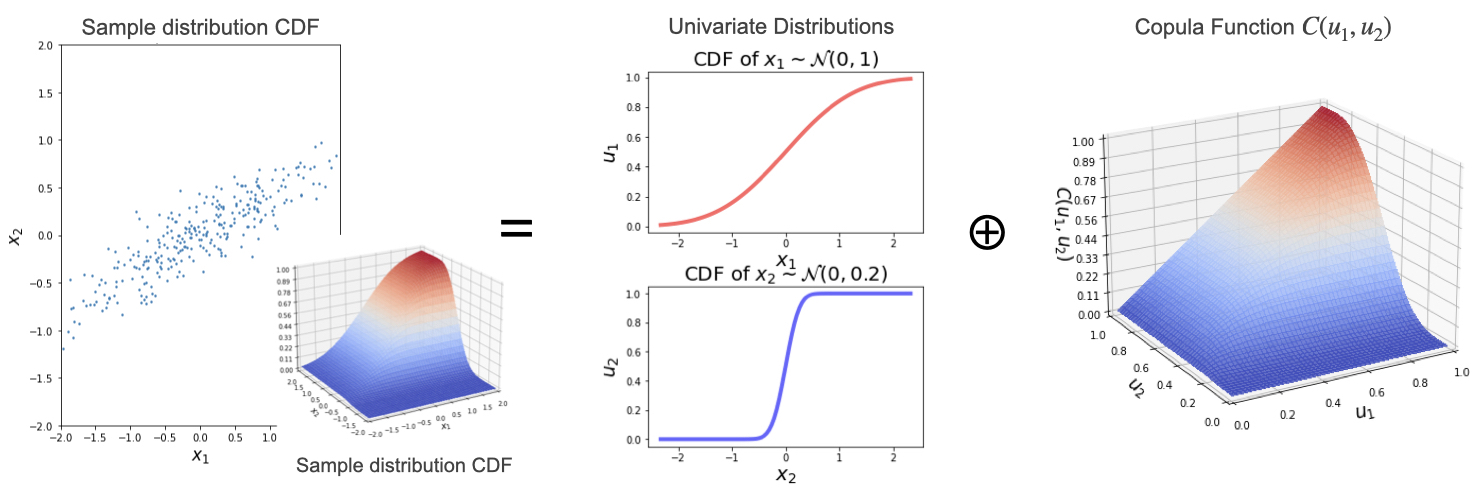
\includegraphics[width=\linewidth]{copula/figs/copula.jpeg}
    \caption{An example copula, where we express a multivarite Gaussian with correlation $\rho = 0.8$ with two univariate distributions and a Copula function $C(u_1, u_2)$.} 
    \label{fig:copula}
\end{figure}



\section{Copula Conformal Prediction for Time Series (CopulaCPTS)}

Many real world decision making tasks make use of time series forecasts that are multivariate and can predict multiple steps into the future. In these applications, we want a "cone of uncertainty" that covers the entire course of our forecasts. Existing time series conformal prediction methods either only provide coverage guarantee for individual time step forecasts \cite{gibbs2021adaptive, xu2021conformal} or produce confidence regions often too inefficient to be useful, especially in multivariate settings  \cite{Schaar2021conformaltime}. Hence, we propose a multi-step conformal prediction algorithm for time series, CopulaCPTS, that guarantees validity over multi-step forecasts. We improve efficiency of the confidence regions by modeling dependency of the time steps using a copula function.

We denote the time series dataset as $\mathcal{D} = \{ (\mathbf{x}_{1:t}^{(i)}, \mathbf{y}_{t+1:t+k}^{(i)}\}_{i=1}^l$, where $\mathbf{x}_{1:t} \in \R^{t\times d_x} $ is $t$ \edit{time steps} of input which has dimension $d_x$, $\mathbf{y}_{t+1:t+k}  \in  \R^{t\times d_y}$ is $k$ \edit{time steps} of output of dimension $d_y$. In the traditional time series forecasting setting we have $d_x = d_y$, but they do not have to be necessarily equal. Given the dataset $\mathcal{D}$, a new test sample $\mathbf{x}_{1:t}^{(n+1)}$, and a confidence level $1-\alpha$, our algorithm returns $k$ confidence intervals, $[\Gamma^{1-\alpha}_1, \ldots, \Gamma^{1-\alpha}_k]$, one for each \edit{time step}, such that:

\begin{equation}
    \mathbb{P}[\: \forall h \in \{1,\ldots, k\}, \: \mathbf{y}_{t+h} \in \Gamma^{1-\alpha}_h\: ] \geq 1-\alpha
\label{eq:tsvalidity}
\end{equation}

for any underlying predictive model. We define equation \ref{eq:tsvalidity} as the \textit{validity} condition for the multi-step time series setting. We will use superscript $\mathbf{x}^i$ to index data, and subscript $\mathbf{y}_t$ to index the time steps within the multi-horizon $\mathbf{y}$.

There are two characteristics desired in uncertainty quantification methods: \textit{calibration} and \textit{efficiency}. A model is calibrated when the predicted confidence level corresponds to the probability of events falling into the predicted range. It is reflected when equality holds in the validity condition $ \mathbb{P} (\mathbf{y} \in \Gamma^{1-\alpha})= 1-\alpha$. \textit{Efficiency}, on the other hand, refers to the size of the confidence region. There is a trade-off between validity and efficiency, as one can always set $\Gamma^{1-\alpha}$ to be infinitely large to satisfy the validity condition. In practice, we want to achieve that the measure of the confidence region (e.g. its area or length) to be as small as possible, given that the validity condition holds. In the following sections we will introduce CopulaCPTS, a conformal prediction algorithm that is both calibrated and efficient for multivariate time series forecasts. 

\subsection{Inductive Conformal Prediction (ICP) for multivariate forecasts}

We view the multidimensional target of dimension $d$ as a point in $\mathbb{R}^d$ space, we simply have $\mathbf{Y}_t = \mathbb{R}^d$ for each \edit{time step} $t$. In this paper we chose nonconformity score to be the L-2 distance $ A((x,y), \hat{f}): = \|y -\hat{f}(x)\|$, where $\hat{f}$ is the forecast model trained on the proper training set $\mathcal{D}_{\text{train}}$. The confidence region $\Gamma^{1-\alpha}(\mathcal{D},x)$ therefore is a $d$-dimensional ball. We chose this  metric because we are forecasting trajectories in space. Since the conformal prediction algorithm produces valid confidence regions regardless of the choice of nonconformity score, one can choose other metrics such as Mahalanobis \cite{johnstone2021conformal} or L-1 \cite{messoudi2021copula} distance based on domain needs, and our algorithm will still hold. 

\subsection{Copula multi-step conformal regression}

We showed in section 3.1 that given a confidence level $1-\alpha$ and a forecast model $\hat{f}$, the ICP algorithm finds a nonconformity score $s_{1-\alpha}$ such that for a new sample $z$ drawn from the data distribution $z \sim \gP$:
\[
	\Prob(A(z, \hat{f}) \leq s_{1-\alpha} ) \geq 1-\alpha
\]

We can use the algorithm to estimate an empirical cumulative distribution function (CDF) for the random variable $A(z, \hat{f})$.

\begin{equation}
    \hat{F}(s) := \Prob (A(z, \hat{f})\leq s) = \frac{1}{|D_{cal}|} \sum_{z^i \in D_{cal} } \mathbbm{1}_{A(z^i, \hat{f}) \leq s} 
    \label{eq:cdf}
\end{equation}
	
% With the inverse of the CDF being the same as the empirical quantile estimation (equation \ref{eq:quantile}).
% \begin{equation}
%     \hat{F}^{-1}(p) := \inf\{s: (\frac{1}{|D_{cal}|} \sum_{z^i \in D_{cal} } \mathbbm{1}_{A(z, \hat{f}) \leq s}) \geq p \}
%     \label{eq:inverse_cdf}
% \end{equation}

For the multi-step conformal prediction algorithm, we will estimate this empirical CDF for each step of the time series, denoted as 
\begin{equation}
      \hat{F}_\edit{h}(s_\edit{h}) := \Prob(A(z_\edit{h}, \hat{f}) \leq s_t) \;  \text{for } h \in 1, \ldots, k
\end{equation}

% changed for reviewing
% We want to find a \edit{set of} significance levels $1-\alpha_\edit{h}$, \edit{one} for each prediction time step $ 1,\ldots, k$, such that the entire predicted time-series trajectory is covered by the intervals with confidence $1-\alpha$. We denote these significance levels as $1-\alpha_1, \ldots, 1-\alpha_k$. Following Sklar's theorem, we have:
%
% \begin{equation}
%         F(s_1, \ldots, s_k) = C(F_1(s_1), \ldots, F_k(s_k))
%     = C(1-\alpha_1, \ldots, 1-\alpha_k)
%     = 1 - \alpha
% \end{equation}

\edit{Let $1-\alpha_h$ denote the probability produced by the each time step's CDF function $F_h(s_h), \; h\in 1, \ldots, k$. By Sklar's theorem, we have:}
\begin{equation}
        F(s_1, \ldots, s_k) = C(F_1(s_1), \ldots, F_k(s_k))
    = C(1-\alpha_1, \ldots, 1-\alpha_k)
\end{equation}

\edit{We want to find the set of confidence levels $1-\alpha_h$, such that the entire predicted time series trajectory is covered by the intervals with confidence $1-\alpha$, i.e. $C(1-\alpha_1, \ldots, 1-\alpha_k) \geq 1-\alpha$.} The purpose of using copula is to model the dependency between the multiple predicted time steps, so we can better capture the confidence region for the joint probability. This allows our algorithm to produce more efficient confidence regions. We estimate the copula $C$ with the calibration set $\mathcal{D}_{cal}$, and then we can search for values $\edit{\alpha_h}$ for each time step to obtain the desired multi-step coverage. 

We adopt the empirical copula \edit{\cite{empiricalcop1}} as our default copula. One may pick other parametric copula functions, such as the Gaussian copula, to introduce inductive bias and improve sample efficiency when calibration data is scarce.  The empirical copula is a non-parametric method of estimating marginals directly from observation, and hence does not introduce any bias. For the joint distribution of a time series with $k$ \edit{time steps}, the copula of a vector of probabilities $\mathbf{u} \in [0,1]^k$ is defined as
\begin{equation}
C_{\text{empirical}} (\mathbf{u}) =  \frac{1}{n-m}\sum_{i=m+1}^{n} \mathbbm{1}_{\mathbf{u}^i <\mathbf{u}} = \frac{1}{n-m}\sum_{i=m+1}^{n} \prod_{h=1}^{k}  \mathbbm{1}_{\mathbf{u}^i_h <\mathbf{u}_h}
\label{eq:empiricalcopula}
\end{equation}

Where $n-m$ is the size of the calibration set. Here, the $\mathbf{u}_i$s are the cumulative probabilities for each data in the calibration set $\mathcal{D}_{cal}$ with size $n-m$. 
\[
     \mathbf{u}^i = (u^i_1, \ldots, u^i_k) = (\hat{F}_1(s^i_1), \ldots, \hat{F}_1(s^i_k)), \; i\in \{m+1, \ldots, n\} 
\]


\edit{We make the assumption that $C_{empirical}$ is an accurate copula function for the prediction horizon.} To fulfill the validity condition of \autoref{eq:tsvalidity}, we only need to find  
\begin{equation}
     \mathbf{u^*}=(\hat{F}_1(s^*_1), \ldots, \hat{F}_t(s^*_k)) \; \text{such that } \; C_{\text{empirical}} (\mathbf{u^*}) \geq 1-\alpha
\label{eq:search}
\end{equation}

We can find  $s_1^*, \ldots, s_k^*$ through any search algorithm. As exhaustive search is exponential to the prediction horizon $k$, we implement the search with stochastic gradient descent using PyTorch. \edit{We study the effectiveness of this method in Appendix C.6}. The confidence region for each \edit{time step} is constructed as the set of all $y_t \in \textbf{y}_t$ such that the nonconformity score is less than $s_t^*$. Algorithm \ref{alg:cpts} summarizes the CoupulaCPTS procedure. \edit{We prove that CopulaCPTS produces valid confidence regions for multi-step time series forecasting (Proposition \ref{lem:copulavalid}) in Appendix \ref{app:proof}.}

\begin{algorithm}[t!]
    \SetKwInput{Input}{Input}
    \SetKwInput{Output}{Output}
    \Input{Dataset $\gD = {(x_i, y_i)}_{i = 1, \ldots, n}$, test input $\mathbf{x}_{1:t}^{n+1}$, target significant level $1-\alpha$.}
    \Output{Confidence regions $\Gamma^{1-\alpha}_1, \ldots,\Gamma^{1-\alpha}_k$.}
    \hrulefill\\
    \tcp{Training}
    Randomly split dataset $\gD$ into training and calibration datasets $\gD = \Dtrain \cup \Dcal$, where $|\Dtrain| = m$ and $|\Dcal| = n-m$.\\
    Train $k$-step forecasting model $\hat{f}$ with   training set $\Dtrain$.\\
    % calibration
    \tcp{Calibration}
    Initialize set of nonconformity scores for each \edit{time step} $\mathcal{S}_h = \emptyset$ for $h=1,\ldots,  k$.\\
    % get nonconformity scores
    \For{$(\mathbf{x}_{1:t}^i, \mathbf{y}_{t+1:t+k}^i) \in \mathcal{D}_{cal} $}{
        $\hat{\mathbf{y}}_{t+1:t+k}^{i} \leftarrow \hat{f}(\mathbf{x}_{1:t}^{i})$ \\
        \For{ $h=1$ \KwTo $k$}{
        $\mathcal{S}_h \leftarrow \mathcal{S}_h \bigcup \|\hat{\mathbf{y}}_{t+h}^{i} - \mathbf{y}_{t+h}^{i}\|$
        }
    }
    % to revise
    Construct CDFs $\hat{F}_1 \ldots \hat{F}_k$ as equation \ref{eq:cdf}. \\
    Construct copula $C(\hat{F}_1(\cdot), \ldots, \hat{F}_k(\cdot))$ as equation \ref{eq:empiricalcopula}.\\
    %give alpha a different name
     Search for $s^*_1, \ldots, s^*_k$  such that $C(\hat{F}_1(s^*_1), \ldots, \hat{F}_k(s^*_k)) \geq 1-\alpha$\\
    %for new time series
    \tcp{Prediction}
    $\hat{\mathbf{y}}^{n+1}_{t+1:t+k} \leftarrow \hat{f}(\mathbf{x}_{1:t}^{n+1})$ \\
    \For{ $h=1$ \KwTo $k$}{
     $\Gamma_h \leftarrow \{ \mathbf{y} : \;  \|\mathbf{y} - \hat{\mathbf{y}}^{n+1}_h \| < s^*_h \} $ \\
    } 
     \KwRet{$\Gamma^{1-\alpha}_1, \ldots,\Gamma^{1-\alpha}_k$}
 \caption{Copula Conformal Time Series Prediction}
 \label{alg:cpts}
\end{algorithm}

% It is simple to show that CopulaCPTS produces valid confidence regions for multi-step time series forecasting. Observe that the empirical copula $C_{\text{empirical}}$ (eq. \ref{eq:empiricalcopula}) itself can be viewed as a way to rank the multi-dimensional nonconformity score. Therefore, the validity proof of inductive conformal prediction (Equation \ref{eq:validityproof}, \ref{eq:region} \cite{vovk2005algorithmic}) holds. See Appendix \ref{app:proof} for the proof of Proposition \ref{lem:copulavalid}.

\begin{proposition}[Validity of CopulaCPTS]
The confidence regions provided by CopulaCPTS (algorithm \ref{alg:cpts}) are valid. i.e. $ \edit{\Prob}[\: \forall h \in \{1,\ldots, k\}, \: \mathbf{y}_{t+h} \in \Gamma^{1-\alpha}_h\: ] \geq 1-\alpha$.
\label{lem:copulavalid}
\end{proposition}

% \\&= (1-\epsilon)
% ( Since \hat{F}_1(s^{n+1}_i) \geq \hat{F}_1(s^*_i) \text{ for all } i ) \quad

\subsection{CopulaCPTS in  auto-regressive forecasting }
Auto-regressive forecasting is a common framework in time series forecasting. So far, we've been looking at forecasts for a predetermined number of \edit{time steps} $k$. One can use a fixed length model to forecast for longer horizons $k'$ autoregressively - by taking model output as part of the input. In the conformal prediction setting, we want to not only to autoregressively use the point value forecasts, but also propagate the uncertainty measurement. 

If we assume the time series to be \textit{stationary}, then the copula remains the same for any sliding window of $k$ steps, i.e. $C(u_1, \ldots, u_k) = C(u_2, \ldots, u_{k+1})$. Given a model $\hat{f}$ to predict $k$ time steps. Hence, after we've found the $u_1^*, \ldots, u_k^*$ such that $C(u_1^*, \ldots, u_k^*) \geq 1-\alpha$, we simply have to search for $u_{k+1}^*$ such that $C(u_2^*, \ldots, u_k^*, u_{k+1}^*) \geq 1-\alpha$. The guarantee proven in Proposition \ref{lem:copulavalid} still holds for the new estimation. On the other hand, if the time series is \textit{non-stationary}, we can fit copulas $C_1(u_1, \ldots, u_k)$, $\ldots$, $C_{k'-k}(u_{k'-k}, \ldots, u_{k'})$, one for each autoregressive prediction, given that we have $k'$ steps of data in our calibration set. This way, we transform the autoregressive problem into $k'-k$ multi-step problems that can be solved by CopulaCPTS. It follows that each of the autoregressive predictions are valid. Appendix \ref{lab:autoregressive} provides an example scenario where re-estimating the copula is necessary and improves validity.


\section{Experiments}
In this section, we show that CopulaCPTS produces more calibrated and efficient confidence regions compared to existing methods on two synthetic datasets and two real-world datasets. We also demonstrate that CopulaCPTS's advantage is more evident over longer prediction horizons. We also show its effectiveness in the autoregressive prediction setting.

\paragraph{Baselines.} We compare our model with three representative works in different paradigms of uncertainty quantification for neural network time \edit{series} prediction: the Bayesian-motivated Monte Carlo dropout RNN (MC-dropout) by \cite{gal2016dropout}, the frequentist blockwise jackknife RNN (BJRNN) by \cite{bjrnn}, and a conformal forecasting RNN (CF-RNN) by \cite{Schaar2021conformaltime}. We use the same underlying prediction model for post-hoc uncertainty quantification methods BJRNN, CF-RNN, and CopulaCPTS. The MC-dropout RNN is of the same architecture but is trained separately, as it requires an extra dropout step during training and inference. 
%We also compare CF-RNN and CopulaCPTS with an encoder-decoder neural network model as the underlying predictor, to showcase the versatility and robustness of our algorithm. We denote these models as CF-\{\texttt{model name}\}, and copula-\{\texttt{modle name}\}.

\paragraph{Metrics.}
We evaluate calibration and efficiency for each method. For calibration, we report the empirical coverage on the held-out test set. Coverage should be as close to the desired confidence level $1-\alpha$ as possible. Coverage is calculated as $coverage_{1-\alpha} =  \mathbb{E}_{x,y \sim \mathbf{X} \edit{\times} \mathbf{Y}} P(\mathbf{y} \in \Gamma^{1-\alpha}(\mathbf{x})) \approx \frac{1}{n} \sum^n_1 \mathbbm{1} (\mathbf{y}_n \in \Gamma^{1-\alpha}_n(\mathbf{x}_n)\edit{)}$. For efficiency, we report the average area (2D) or volume (3D) of the confidence region. The metric should be as small as possible while being valid (coverage maintains above pre-specified confidence level). The area or volume is calculated as $area_{1-\alpha} = \mathbb{E}_{x \sim \mathbf{X}} \|\Gamma^{1-\alpha}(x)\|  \approx \frac{1}{n} \sum^n_1 \|\Gamma^{1-\alpha}(x_n)\|$.


\subsection{Synthetic Datasets}

We first test the effectiveness of our models with two synthetic spatiotemporal datasets - interacting particle systems \edit{\cite{nridataset}}, and drone trajectory following (simulated with PythonRobotics \edit{\cite{pythonrobotics}}). For the particle simulation we predict $\mathbf{y}_{t+1:t+h}$ where $t=35$, $h=25$ and $y_t \in \mathbb{R}^2$; for drone simulation $t=60$, $h=10$, and $y_t \in \mathbb{R}^3$. To add randomness to the tasks, we added Gaussian noise of $\sigma = .01$ and $.05$ to the dynamics of the particle simulation, and $\sigma = .02$ to drone dynamics. \edit{We generate 5000 samples for each dataset, and split the data by 45/45/10 for train, calibration, and test respectively. Please see Appendix C.1 for forecaster model details.}

We visualize the calibration and efficiency of the methods in \autoref{fig:synthetic} for confidence levels $1-\alpha = 0.5$ to $0.99$. We can see that Copula-RNN, the red lines, are more calibrated and efficient compared to other baseline methods, especially in tasks with large noise (particle dataset, $ \sigma = 0.05$). We can see that for harder tasks (particle $ \sigma = 0.05$, and drone trajectory prediction), MC-Dropout is overconfident, whereas BJ-RNN and CF-RNN produce very large (hence inefficient) confidence regions. This behavior of CF-RNN is expected because they apply Bonferroni correction to account for joint prediction for multiple time steps, which is an upper bound of copula functions. The numbers for confidence level $90\%$ are presented in Table \ref{tab:baselines_new}. A quantitative comparison of confidence regions for drone simulation can be found in Figure \ref{fig:drone} in the appendix.

\begin{figure}[h]
    \centering
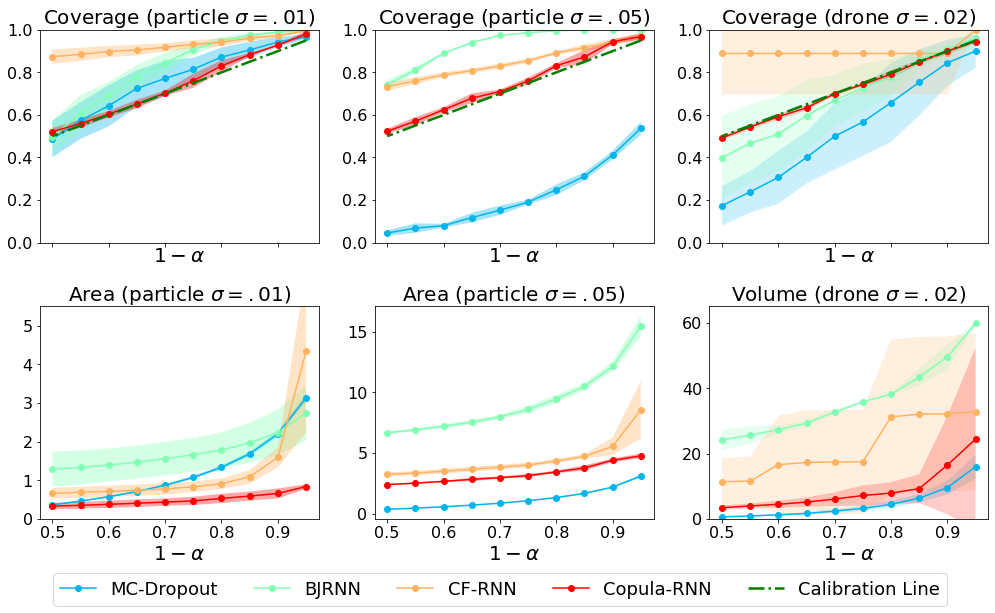
\includegraphics[width=0.9\linewidth]{copula/figs/synthetic_update.png}
    \caption{Calibration (upper row) and efficiency (lower row) comparison on different $1-\alpha$ levels for simulated data sets. For calibration, the goal is to coincide with the green dotted calibration line as closely as possible while staying valid (above the green line). Note that copula methods are more calibrated across different significance levels. For efficiency, we want the metric to be as low as possible. Copula-RNN outperforms the baselines consistently. (MC-dropout for the right two experiments produces invalid regions, so we don't consider its efficiency.)}
    \label{fig:synthetic}
\end{figure}


% ---------------------------------
% updated table
% ---------------------------------
\begin{table}
\centering
\begin{tabular}{ c | c | c  c c  c  } 
 \toprule
 & & MC-dropout & BJRNN & CF-RNN & Copula-RNN \\
\midrule\midrule
 \multirow{2}{*}{\begin{tabular}{l}Particle Sim \\ ($\sigma=.01$)\end{tabular}} & Coverage  & \color{gray}{  63.9 \plusminus 16.1  } &   98.9 \plusminus 0.2   &   97.0 \plusminus 2.3   & \textbf{  91.5 } \plusminus 2.1   \\ 
 & Area  & \color{gray}{  0.81 \plusminus 0.05  } &   2.24 \plusminus 0.59   &   3.13 \plusminus 3.24   &  \textbf{1.06}  \plusminus 0.36   \\ \midrule  
 \multirow{2}{*}{\begin{tabular}{l}Particle Sim\\ ($\sigma=.05$)\end{tabular}} & Coverage  & \color{gray}{  16.1 \plusminus 4.3  } &   100.0 \plusminus 0.0   &   94.5 \plusminus 1.5   & \textbf{  90.3} \plusminus 0.7   \\ 
 & Area  & \color{gray}{  0.79 \plusminus 0.02  } &   12.13 \plusminus 0.39   &   5.79 \plusminus 0.51  & \textbf{  4.50 } \plusminus 0.07   \\ \midrule  
 \multirow{2}{*}{\begin{tabular}{l}Drone Sim\\ ($\sigma=.02$)\end{tabular}} & Coverage  & \color{gray}{  84.5 \plusminus 10.8  } &   90.8 \plusminus 2.8   &   91.6 \plusminus 9.2   &  \textbf{90.0} \plusminus 1.5  \\ 
 & Volume  & \color{gray}{  9.64 \plusminus 2.13 } &   49.57 \plusminus 3.77  &   32.18 \plusminus 13.66  &  \textbf{16.52}  \plusminus 7.08  \\
 \midrule\midrule
 \multirow{2}{*}{\begin{tabular}{l}COVID-19 \\ Daily Cases \end{tabular}} & Coverage  & \color{gray}{ 19.1 \plusminus 5.1 } &  \color{gray}{ 79.2 \plusminus 30.8}  &  95.4 \plusminus 1.9  & \textbf{ 92.1} \plusminus 1.0  \\ 
 & Area  & \color{gray}{ 34.14 \plusminus 0.84  } &  \color{gray}{ 823.3 \plusminus 529.7}  &  610.2 \plusminus 96.0  & \textbf{429.0} \plusminus 15.1  \\   \midrule 
 \multirow{2}{*}{\begin{tabular}{l}Argoverse \\ Trajectory \end{tabular}} & Coverage  & \color{gray}{ 27.9 \plusminus 3.1 } &  92.6 \plusminus 9.2  &  98.8 \plusminus 1.9  &  \textbf{90.4} \plusminus 0.3 \\ 
 & Area  & \color{gray}{ 127.6 \plusminus 20.9 } &  880.8 \plusminus 156.2  &  396.9 \plusminus 18.67  &  \textbf{126.8} \plusminus 12.22 \\  
\bottomrule
\end{tabular}
\caption{Performance on synthetic and real world datasets with target confidence $1-\alpha = 0.9$. Methods that are \textit{invalid} (coverage below $90\%$) are greyed out. CopulaCPTS achieves high level of calibration (coverage is close to $90\%$) while producing more efficient confidence regions (small area).} 
\label{tab:baselines_new}
\end{table}


% ---------------------------------
% real world dataset
% ---------------------------------

\subsection{Real world datasets}
%We choose two scenarios in the real world where calibrated and sharp uncertainty quantification are important. 

\textbf{COVID-19.} We replicate the experiment setting of \cite{Schaar2021conformaltime} and predict new daily cases of COVID-19 in regions of the UK. The models take 100 days of data as input and forecast 50 days into the future. We used 200 time series for training, 100 for calibration, and 80 for testing.

\textbf{Vehicle trajectory prediction.} The Argoverse autonomous vehicle motion forecasting dataset \cite{argoverse} is a widely used vehicle trajectory prediction benchmark. The task is to predict 3 second trajectories based on all vehicle motion in the past 2 seconds sampled at 10Hz. Because trajectory prediction is a challenging task, we utilize a state-of-the-art prediction algorithm LaneGCN \cite{liang2020learning} as the underlying model for CF-RNN and Copula-RNN \edit{(details in Appendix C.1)}. Flexibility of underlying forecasting model is an advantage of post-hoc conformal prediction methods. \edit{For model-dependent baselines MC-dropout and BJRNN, we have to train an RNN forecasting model from scratch for each method, which is additional computational cost.} 
%We re-train an encoder-decoder RNN model for MC-dropout and BJRNN which are more computationally heavy.

Results in Table \ref{tab:baselines_new} show that, like for synthetic datasets,  CopulaCPTS is both more calibrated and efficient compared to baseline models for real world datasets. For the trajectory prediction task, learning the copula results in a $77\%$ sharper confidence region while still remaining valid for the $90\%$ confidence interval. We visualize two samples from each dataset in Figure \ref{fig:realworld}.
The importance of efficiency in these scenarios is clear - the confidence regions need to be narrow enough for them to be useful for decision making. Given the same underlying prediction model, we can see that CopulaCPTS produces a much sharper region while still remaining valid.

\begin{figure}
\centering
\begin{subfigure}{.245\textwidth}
  \centering
  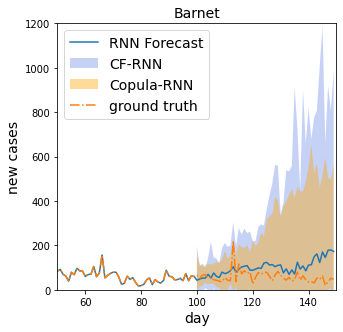
\includegraphics[width=\linewidth]{copula/figs/covidnew1.png}
  \label{fig:cov001}
\end{subfigure}%
\begin{subfigure}{.245\textwidth}
  \centering
  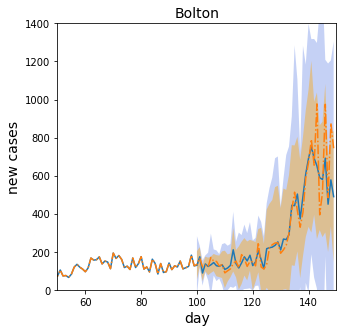
\includegraphics[width=\linewidth]{copula/figs/covidnew2.png}
  \label{fig:cov002}
\end{subfigure}
\begin{subfigure}{.245\textwidth}
  \centering
  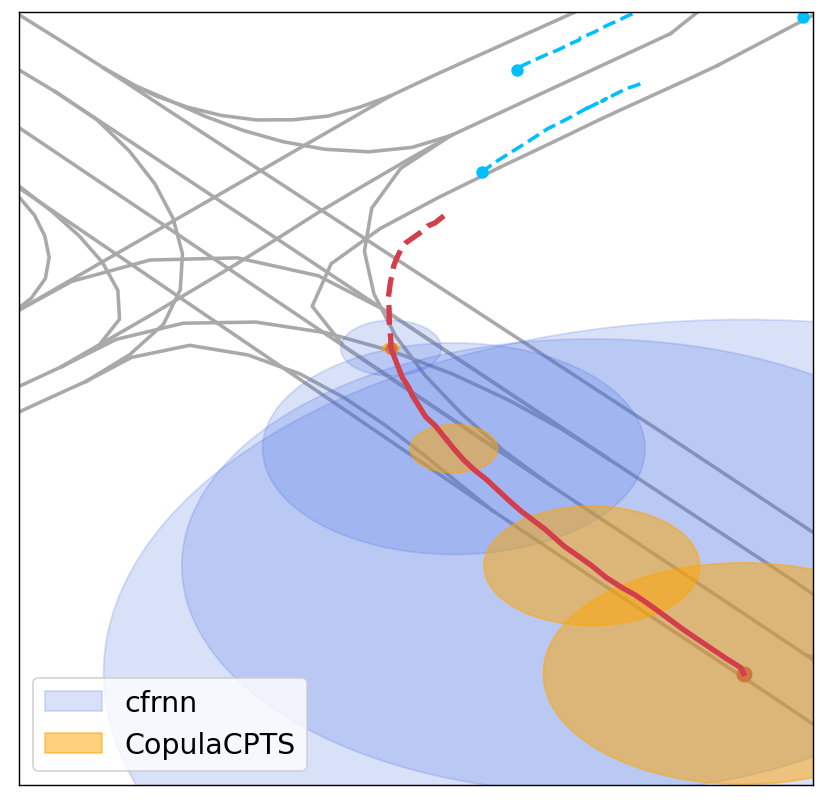
\includegraphics[width=\linewidth]{copula/figs/argoverse1.png}
  \label{fig:conf1}
\end{subfigure}%
\begin{subfigure}{.245\textwidth}
  \centering
  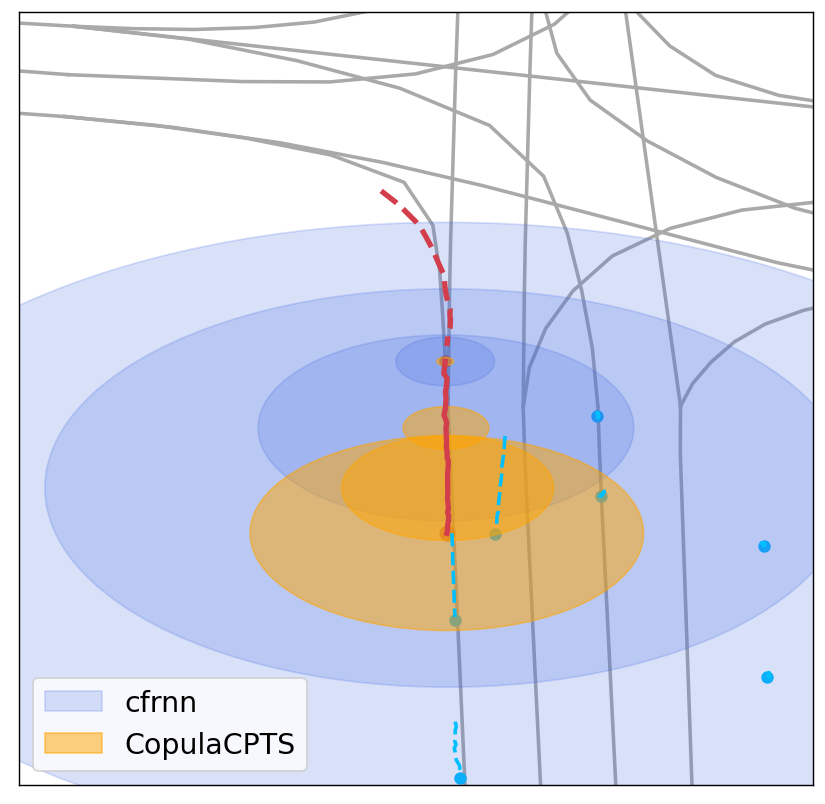
\includegraphics[width=\linewidth]{copula/figs/argoverse2.png}
  \label{fig:conf2}
\end{subfigure}
\caption{Illustrations of 90\% confidence regions given by CF-RNN (blue) and CopulaCPTS (orange) on two real-world datasets. For COVID-19 forecast (left 2) we see that CopulaCPTS produces sharper yet covering confidence regions. For Argoverse (right 2) we illustrate regions at time steps 1, 10, 20, and 30. Note that the confidence region produced CF-RNN is uninformatively large, as it covers all the lanes. Overall, CopulaCPTS is able to produce much more efficient confidence regions while maintaining valid coverage. These examples also  illustrate the importance of efficiency.}
\label{fig:realworld}
\end{figure}

\paragraph{Comparison of models at different horizon lengths.} CopulaCPTS is an algorithm designed to produce calibrated and efficient confidence regions for multi-step time series. When the prediction horizon is long, CopulaCPTS's advantage is more pronounced. Figure \ref{fig:horizon} shows performance comparison across increasing time horizons on the particle dataset. See Table \ref{tab:baselines} of Appendix \ref{app:exp_details} for additional experiment results. CopulaCPTS achieves a $30\%$ decrease in area at 20 time steps compared to CF-RNN, the best performing baseline; the decrease is above $50\%$ at 25. This experiment shows significant improvement of using copula to model the joint distribution of future time steps. 

\paragraph{CopulaCPTS for the Autoregressive prediction setting.} We test the autoregressive setting (section 4.3) on the COVID-19 dataset. We train an RNN model with $k=7$ and use it to autoregressively forecast the next 14 steps. Table \ref{tab:autoregressive} compares the performance of re-estimating the copula for each 7-step forecasts versus using a fixed copula calibrated using the first 7 steps. We compare the model to a 14-step joint forecaster using CopulaCPTS as well.  

\begin{figure}
    \centering
    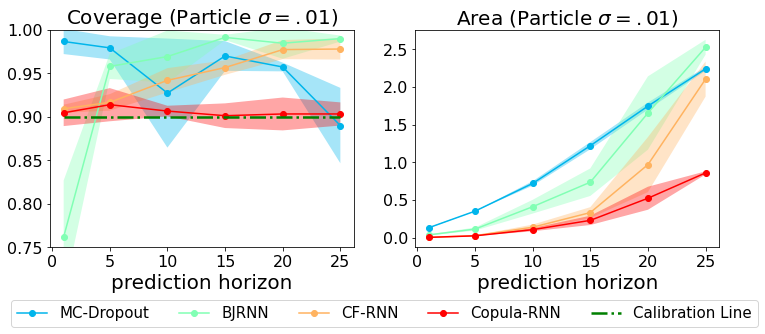
\includegraphics[width=0.6\textwidth]{copula/figs/horizon01.png}
\captionof{figure}{CopulaCPTS remains more calibrated and efficient than baselines over increasing forecast horizons.}
\label{fig:horizon}
\end{figure} 

\begin{table}
    \centering
    \begin{tabular}{c|c|c}
    \toprule
    Method & Coverage & Area \\
          \midrule\midrule
    AR re-estimate  & \textbf{90.7}  & \textbf{377.9} \\
    AR fixed  & 88.2  & 340.5 \\
    Joint & 90.8 & 429.4\\
         \bottomrule
    \end{tabular}
    \captionof{table}{Performance of autoregressive (AR) CopulaCPTS.  Re-estimating copula gives us valid confidence region over time and is more efficient than joint CopulaCPTS forecast.}
    \label{tab:autoregressive}
\end{table} 




\section{Conclusion and Discussion}
In this paper we present CopulaCPTS, a conformal prediction algorithm for multidimensional and multi-step time-series prediction. CopulaCPTS significantly improves calibration and efficiency of multi-step conformal confidence intervals by incorporating copulas to model the joint distribution of multiple timesteps. We prove that CopulaCPTS has finite sample validity guarantee. In our experiments we show that the algorithm outperforms state-of-the-art models on all 4 benchmark datasets and on varying prediction horizons. On the flip side, CopulaCPTS assumes that the copula estimation is accurate and we have calibration data for the entirety of the prediction horizon, even in the autoregressive case. We leave it to future work to relax these assumptions (for example by adjusting $\mathbf{u}^*$ online given prediction errors as in \cite{gibbs2021adaptive}) to make CopulaCPTS applicable to the online setting where distribution shift is present.


\section{Proof of Proposition \ref{lem:copulavalid}}
\label{app:proof}
\begin{prop*}[Validity of CopulaCPTS]
The confidence region provided by CopulaCPTS (algorithm \ref{alg:cpts}) \edit{is} valid. i.e. $ \edit{\Prob}[\: \forall h \in \{1,\ldots, k\}, \: \mathbf{y}_{t+h} \in \Gamma^{1-\alpha}_h\: ] \geq 1-\alpha$.
\end{prop*}

\begin{proof}
We assume that our estimation of $C_{\text{empirical}}$ is accurate. Via search, we found  $\mathbf{u^*} = (\hat{F}_1(s^*_1), \ldots, \hat{F}_t(s^*_k))$ such that
\begin{align}
    C_{\text{empirical}} (\mathbf{u^*}) = \displaystyle \mathop{\mathbb{E}}_\textbf{u}  \prod_{t=1}^{k}  \mathbbm{1}_{\mathbf{u}^*_t <\mathbf{u}_t} \geq 1-\alpha
\end{align}
Let $(\mathbf{x}_{1:t}^{n+1}, \mathbf{y}_{t+1:t+h}^{n+1}) \sim \mathbf{X}\times \mathbf{Y}$ be a new data point. Denote $\hat{\mathbf{y}} = \hat{f}(\mathbf{x}_{1:t}^{n+1})$, the forecast given by the trained model. Because the $\hat{F}_h$ functions and $C_{\text{empirical}}$ are monotonously increasing, we have:
\begin{align*}
    P[\: \forall h \in \{1,\ldots, k\}, \: \mathbf{y}_{t+h} \in \Gamma^{1-\alpha}_h\: ] 
    &= C(\hat{F}_1(s^{n+1}_1), \ldots, \hat{F}_k(s^{n+1}_k))\\
    &\geq  C( \hat{F}_1(s^*_1), \ldots, \hat{F}_k(s^*_k)) \\
    &\geq 1-\alpha
\end{align*} 
\end{proof}


\section{Additional Algorithm Details}

\subsection{Upper and Lower bounds for Copulas}
To provide a better understanding of the properties of Copulas, consider the Frechet-Hoeffding Bounds (Theorem \ref{lem:bounds}). In fact, the Frechet-Hoeffding upper- and lower- bounds are both copulas. The lower bound is percisely the Bonferroni correction used in \cite{Schaar2021conformaltime} - therefore by estimating the copula more precisely instead of using a lower bound, we have a guaranteed efficiency improvement for the confidence region. 

%Copulas can be parametric or non-parametric; the Gaussian copula, for example, is used for pricing in financial markets \cite{Haugh2016copula}. 

\begin{theorem}[The Frechet-Hoeffding Bounds]
Consider a copula $C(u_1, \ldots, u_k)$. Then
\[
\max{\{1-k+\sum_{i=1}^k u_i, 0\} } \leq C(u_1, \ldots, u_k) \leq \min{ \{u_1, \ldots, u_k \}}
\]
\label{lem:bounds}
\end{theorem}

\subsection{Numerical optimization with SGD for search}
The empirical inverse CDF modeled the same way as Equation \ref{eq:cdf} is the same as the empirical quantile estimation (Equation \ref{eq:quantile}).
\begin{equation}
    \hat{F}^{-1}(p) := \inf\{s: (\frac{1}{|D_{cal}|} \sum_{z^i \in D_{cal} } \mathbbm{1}_{A(z, \hat{f}) \leq s}) \geq p \}
    \label{eq:inverse_cdf}
\end{equation}


We find the optimal $s_h^*$ in Equation \ref{eq:search} and Algorithm \ref{alg:cpts} by minimizing the following loss: 
\[
\gL(s_1, \ldots, s_k) = \frac{1}{n-m} \sum_{i=m+1}^{n} \prod_{h=1}^k \mathbbm{1}\left[ \mathbf{u}^i_h < \hat{F}_h^{-1}(s_h) \right] - (1-\alpha) 
\]
We use the Adam optimizer and optimize for 500 steps. An alternative and faster way of search is to assume $s_1 = s_2 = \cdots = s_k$ which simplifies the search from exponential time to constant time. 

\subsection{Autoregressive prediction}
\label{lab:autoregressive}
In the context of this paper to forecast autoregressively is given input $\textbf{x}_{1:t}$ and a $k$ step forecasting model $\hat{f}$, perform prediction

\begin{align*}
    \hat{\textbf{y}}_{t+1:t+k} &= \hat{f}(\textbf{x}_{1:t}) \\
    \hat{\textbf{y}}_{t+2:t+k+1} &= \hat{f}(\textbf{x}_{2:t},  \hat{\textbf{y}}_{t+1}) \\
    & \cdots
\end{align*}

until all $k'$ time steps are predicted. 

We now provide a toy scenario to illustrate when re-estimating the copula is necessary and improves validity. Consider a time series of three time steps $t_0, t_1, t_2$. The two scenarios are illustrated in Figure \ref{fig:ar}. In both scenarios the mean and variance of all timeseps are $0$ and $1$ respectively.  In scenario (a), $t_0 = t_1$ and hence their covariance is $1$. The copula estimated on $t_0$ and $t_1$ is $C_{0:1}(F(t_0), F(t_1)) = F(t_0) = F(t_1)$.  This copula will significantly underestimate the confidence region of  $t_2$ where its covariance with $t_1$ is $-1$. In fact the coverage of $C_{0:1}(F_1(t_1), F_2(t_2)) =0.74 $. On the other hand, (b) illustrates a scenario where the copula for any 2 consecutive time series remain the same $C_0=C_1$. In this case, applying $C_0$ directly to forecast $C_1$ achieves precisely 90\% coverage.


\begin{figure}[h!]
\centering
\begin{subfigure}[b]{0.45\linewidth}
  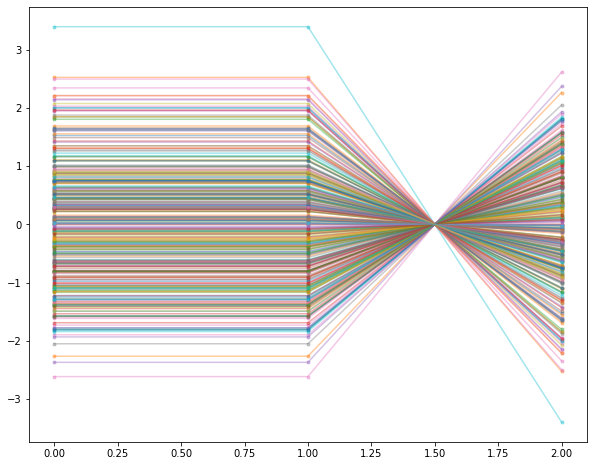
\includegraphics[width=\linewidth]{copula/figs/appscene1.png}
  \caption{Time steps 0 and 1 are positively correlated while 1 and 2 are negatively correlated}
  \label{fig:cal001}
\end{subfigure}
\hspace{0.8em}
\begin{subfigure}[b]{0.45\linewidth}
  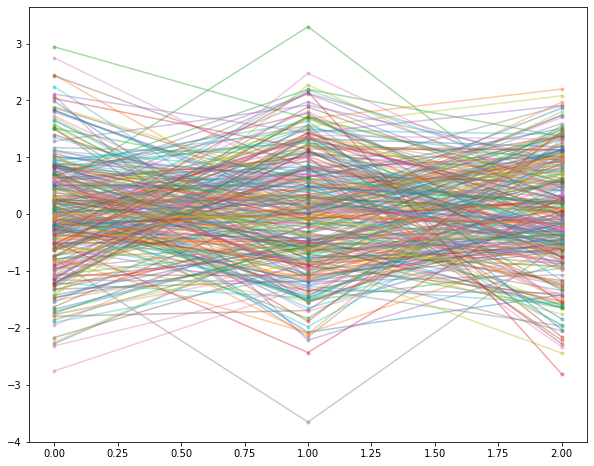
\includegraphics[width=\linewidth]{copula/figs/appscene2.png}
  \caption{Stationary time series where each time steps are uncorrelated}
  \label{fig:cal002}
\end{subfigure}%
\caption{Two scenarios to illustrate the autoregressive case}
\label{fig:ar}
\end{figure}



\section{Experiment Details and additional results}
\label{app:exp_details}

\subsection{Underlying forecasting models}

\edit{
\paragraph{Particle Dataset}
The underlying forecasting model for the particle experiments is an 1-layer LSTM network with embedding size $=24$. The hidden state is then passed through a linear network  to forecast the timesteps concurrently (output has dimension $k \times d_y$).  We train the model for 150 epochs with batch size 128. Hyperparameters of the network are selected through a model search by performance on a 5-fold cross validation split of the dataset. The architecture and hyperparameters are shared for all baselines and CopulaCPTS in Table 1.

\paragraph{Drone} For the drone trajectory forecasting task, we use he same LSTM forecasting network as the particle dataset, but with hidden size increased to 128.  We train the model for 500 epochs with batch size 128. The same architecture and hyperparameters are shared for all baselines and CopulaCPTS reported in Table 1. 

\paragraph{Covid-19} The base forecasting model for Covid-19 dataset is the same as the synthetic datasets, with hidden size $=128$ and were trained for 150 epochs with batch size 128. The same architecture and hyperparameters are shared for all baselines and CopulaCPTS reported in Table 1. 

\paragraph{Argoverse} As highlighted in the main text, we utilize a state-of-the-art prediction algorithm LaneGCN \cite{liang2020learning} as the underlying forcaster model for CF-RNN and Copula-RNN. We refer the readers to their paper and code base for model details. The architecture of the RNN network used for MC-Dropout and BJRNN is an Encoder-Decoder network. Both the encode and decoder contains a LSTM layer with encoding size 8 and hidden size 16. We chose this architecture because the is part of the official Argoverse baselines (\texttt{https://github.com/jagjeet-singh/argoverse-forecasting}) and demonstrates competitive performance.  
}


\subsection{COVID-19 Dataset}
The COVID-19 dataset is downloaded directly from the official UK government website \texttt{https://coronavirus.data.gov.uk/details/download} by selecting \textit{region} for area type and \textit{newCasesByPublishDate} for metric. There are in total 380 regions and over 500 days of data, depending when it is downloaded. We selected 150-day time series from the collection to construct our dataset.


\subsection{Calibration and Efficiency chart for COVID-19}
Figure \ref{fig:covid-day} shows comparison of calibration and efficiency for the daily new COVID 19 cases forecasting. 
\begin{figure}[h!]
    \centering
    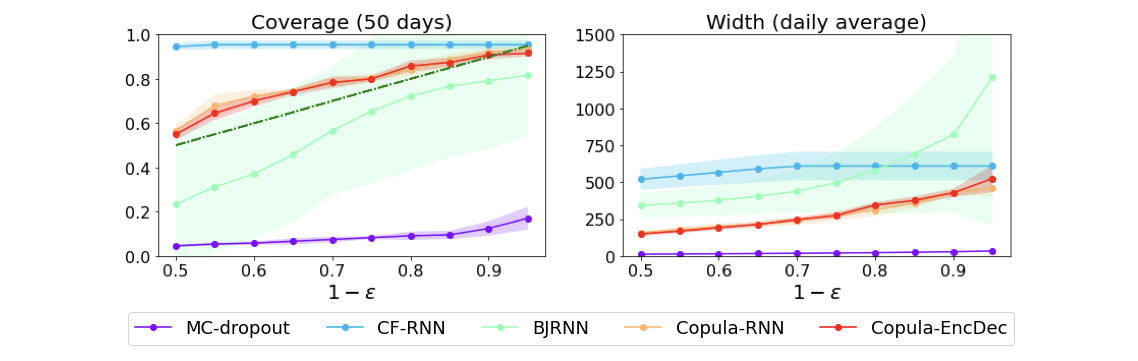
\includegraphics[width=\linewidth]{copula/figs/covid_cov_daily.jpeg}
    \caption{Calibration and efficiency comparison on different $\epsilon$ level for COVID-19 Daily Forecasts. The copula methods (orange and red lines) are more calibrated (coinciding with the green doted line) and sharp (low width) compared to baselines.}
    \label{fig:covid-day}
\end{figure}

To see if the daily fluctuation due to testing behaviour disrupts other method, we also ran the same experiment on weekly aggregated new cases forecast. We take 14 weeks of data as input and output forecasts for the next 6 weeks. The results are illustrated in Figure \ref{fig:covid-week}. The weekly forecasting scenario gives us similar insights as the daily forecasts. 

\begin{figure}[h!]
    \centering
    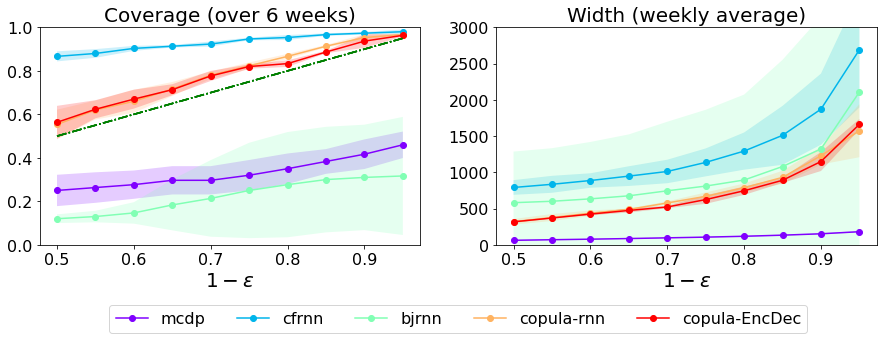
\includegraphics[width=0.8\linewidth]{copula/figs/covidcoverage.png}
    \caption{Covid Weekly Forecasts}
    \label{fig:covid-week}
\end{figure}

\subsection{Argoverse}
The Argoverse autonomous vehicle dataset contains 205,942 samples, consisting of diverse driving scenarios from Miami and Pittsburgh.  The data can be downloaded from the official Argoverse dataset website. We split 90/10 into a training set and validation set of size 185,348 and 20,594 respectively. The official validation set of size 39,472 is used for testing and reporting performance. We preprocess the scenes to filter out incomplete trajectories and cap the number of vehicles modeled to 60. If there are less than 60 cars in the scenario, we insert dummy cars into them to achieve consistent car numbers. For map information, we only include center lanes with lane directions as features. Similar to vehicles, we introduce dummy lane nodes into each scene to make lane numbers consistently equal to 650.

\subsection{Additional Experiment Results}
We present in figure 8 and 9  some qualitative results for uncertainty estimation.  

\edit{ To test how the effects of copulaCPTS compare with baseline on other base forecasters, we also include an encoder-decoder architecture with the same embedding size as the RNN models introduced in appendix C.1 for each dataset. The results are presented in Table \ref{tab:baselines}. We omit these results in the main text because we found that they do did not bring significant improvement to time series forecasting UQ. 

Table \ref{tab:horizon} compares model performance compared across different prediction horizons. We show that the advantage of our method is more pronounced for longer horizon forecasts. 

}

% ---------------------------------
% drone vis
% ---------------------------------


\begin{figure}[h]
\centering
\begin{subfigure}[b]{0.33\linewidth}
  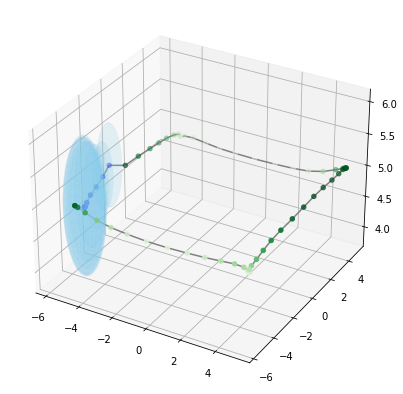
\includegraphics[width=\linewidth]{copula/figs/dronecopula.png}
  \caption{Copula-EncDec}
\end{subfigure}%
\begin{subfigure}[b]{0.33\linewidth}
  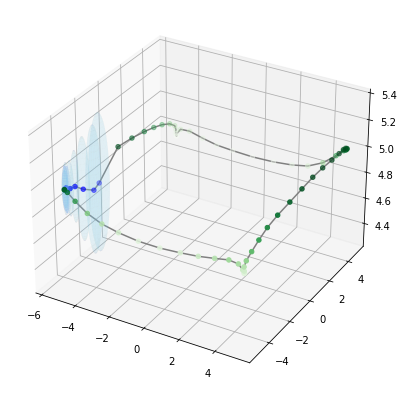
\includegraphics[width=\linewidth]{copula/figs/dronemcdp.png}
  \caption{MC Dropout}
\end{subfigure}%
\begin{subfigure}[b]{0.33\linewidth}
  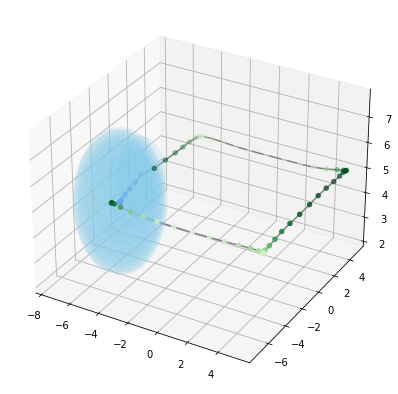
\includegraphics[width=\linewidth]{copula/figs/dronecf.png}
  \caption{CF-RNN}
\end{subfigure}
\caption{ $99\%$ Confidence region produced by three methods for the drone dataset. Copula methods (a) produces a more consistent, expanding cone of uncertainty compared to MC-Dropout (b) sharper one compared to CF-RNN (c). }
\label{fig:drone}
\end{figure}


\begin{figure*}[h!]
\centering
\begin{subfigure}{.245\textwidth}
  \centering
  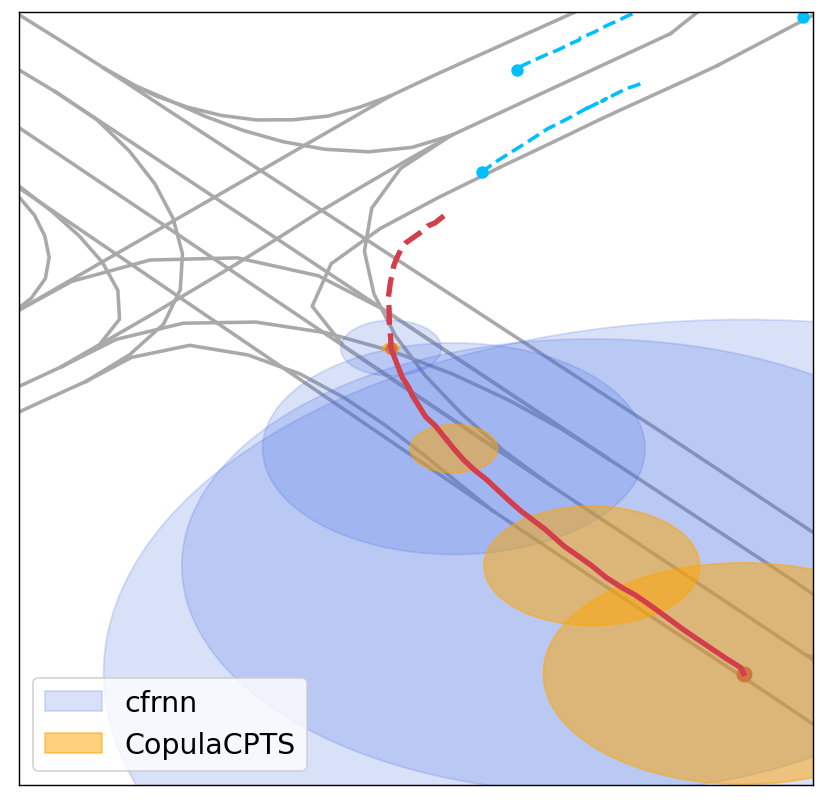
\includegraphics[width=.9\linewidth]{copula/figs/argoverse1.png}
\end{subfigure}%
\begin{subfigure}{.245\textwidth}
  \centering
  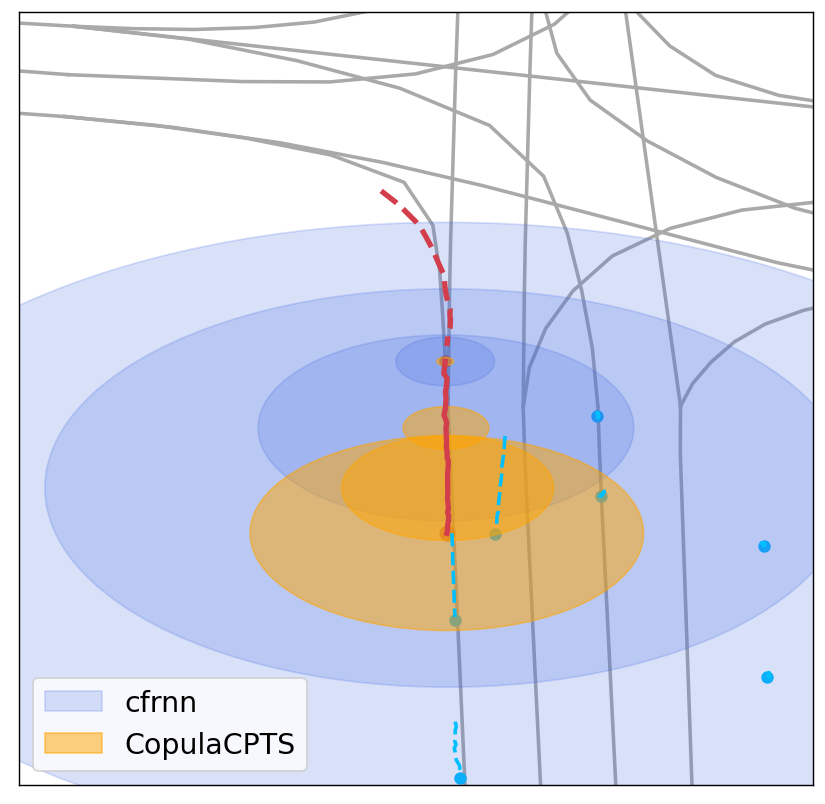
\includegraphics[width=.9\linewidth]{copula/figs/argoverse2.png}
\end{subfigure}
\begin{subfigure}{.245\textwidth}
  \centering
  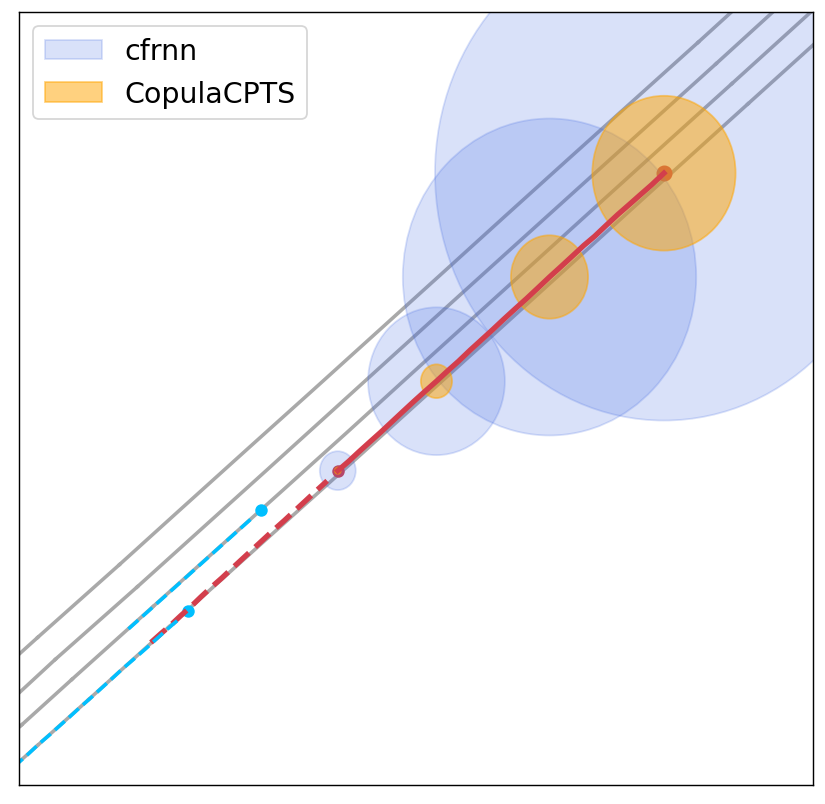
\includegraphics[width=\linewidth]{copula/figs/argoverse3.png}
\end{subfigure}%
\begin{subfigure}{.245\textwidth}
  \centering
  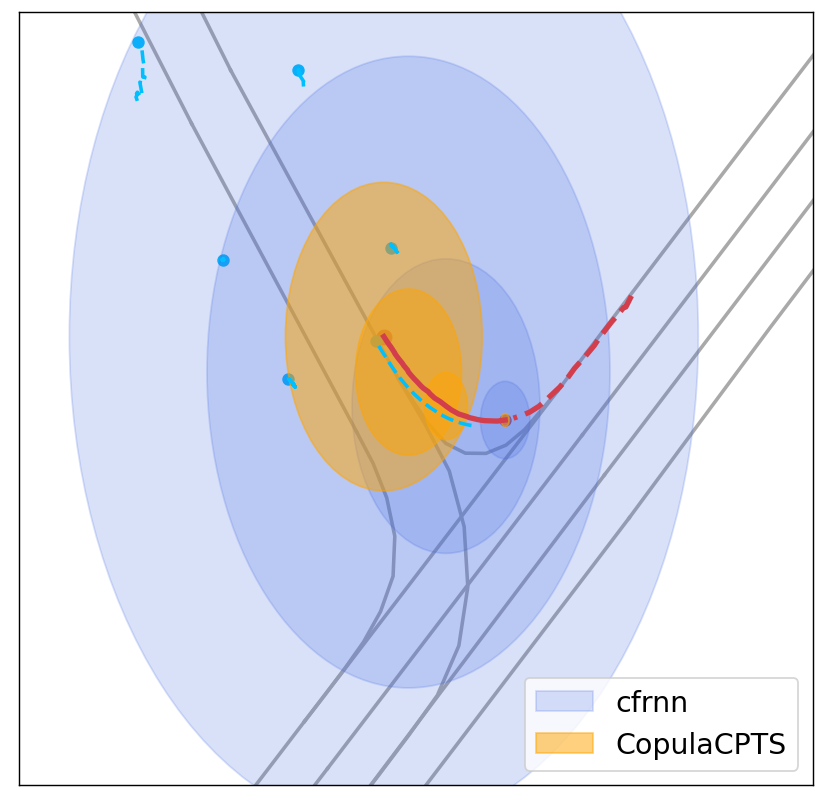
\includegraphics[width=\linewidth]{copula/figs/argoverse4.png}
\end{subfigure}
\caption{Illustrations for confidence regions given by CF-RNN (blue) and CopulaCPTS (orange) in at time steps 0, 10, 20, and 30. Note that in order to achieve 90\% coverage, the regions are larger than needed, especially in straight-lane cases like the middle two. Using copulas to couple together time steps results in a much smaller region, while achieving similarly good coverage.}
\label{fig:argo}
\end{figure*}



% ---------------------------------
% Big big master table
% ---------------------------------
\begin{table*}
\centering
\begin{tabular}{ c | c c  | c c  } 
 \toprule
  \multicolumn{5}{c}{Particle Simulation ($\sigma=.01$)} \\
    \midrule
     & Coverage (90\%) & Area (90\%)   & Coverage (99\%)  & Area (99\%)  \\
  \midrule
    MC-dropout &  63.9 \plusminus 16.1  &  0.81 \plusminus 0.05  &  73.1 \plusminus 14.2  &  1.14 \plusminus 0.07  \\ 
BJRNN &  98.9 \plusminus 0.2  &  2.24 \plusminus 0.59  &   100 \plusminus 0.0  &  3.75 \plusminus 0.71  \\ 
CF-RNN &  97.0 \plusminus 2.3  &  3.13 \plusminus 3.24  &   100  \plusminus 0.21   &   4.34 \plusminus 1.19   \\ 
Copula-RNN &  91.5 \plusminus 2.1  &  \textbf{1.06} \plusminus 0.36  &  97.4 \plusminus 2.4  &  4.47 \plusminus 1.48  \\ 
Copula-EncDec &  \textbf{90.2} \plusminus 2.3  &  1.19 \plusminus 0.17  &  \textbf{99.6} \plusminus 0.7  &  \textbf{1.83} \plusminus 0.09  \\ 
    \midrule
  \multicolumn{5}{c}{Particle Simulation ($\sigma=.05$)} \\
  \midrule 
  & Coverage (90\%) & Area (90\%)   & Coverage (99\%)  & Area (99\%)  \\
  \midrule
  MC-dropout &  16.1 \plusminus 4.3  &  0.79 \plusminus 0.02  &  33.9 \plusminus 5.1  &  2.12 \plusminus 0.03  \\ 
BJRNN &  100.0 \plusminus 0.0  &  12.13 \plusminus 0.39  &  100.0 \plusminus 0.0  &  15.43 \plusminus 0.85  \\ 
CF-RNN &  94.5 \plusminus 1.5  &  5.79 \plusminus 0.51 &  99.8 \plusminus 2.2  &  19.21 \plusminus 8.19  \\ 
Copula-RNN &  \textbf{90.3} \plusminus 0.7  &  4.50 \plusminus 0.07  &  \textbf{99.1} \plusminus 0.8  &  12.82 \plusminus 3.98  \\ 
Copula-EncDec & 91.4 \plusminus 1.1  & \textbf{4.40} \plusminus 0.15  &  98.7 \plusminus 0.1  & \textbf{9.31} \plusminus 1.97  \\ 
    \midrule
  \multicolumn{5}{c}{Drone Simulation ($\sigma=.02$)}\\
  \midrule
   & Coverage (90\%) & Area (90\%)   & Coverage (99\%)  & Area (99\%)  \\
  \midrule
  MC-dropout &  84.5 \plusminus 10.8  &  9.64 \plusminus 2.13 &  90.0 \plusminus 7.8  &  16.02 \plusminus 3.62 \\ 
BJRNN &  90.8 \plusminus 2.8  &  49.57 \plusminus 3.77 &  100.0 \plusminus 4.0  &  65.77 \plusminus 4.56 \\ 
CF-RNN &  91.6 \plusminus 9.2  &  32.18 \plusminus 13.66 &  100.0 \plusminus 0.0  &  36.79 \plusminus 14.03 \\ 
CF-EncDec &  100.0 \plusminus 0.0  &  21.83 \plusminus 26.29 &  100.0 \plusminus 0.0  &  25.03 \plusminus 12.53 \\ 
Copula-RNN &  \textbf{90.0} \plusminus 1.5  &  \textbf{16.52} \plusminus 15.08 &  \textbf{98.5} \plusminus 0.5  &  \textbf{21.48} \plusminus 8.91 \\ 
    \midrule
  \multicolumn{5}{c}{COVID-19 Daily Cases Dataset} \\
  \midrule
    & Coverage (90\%) & Area (90\%)   & Coverage (99\%)  & Area (99\%)  \\
  \midrule
 MC-dropout & 19.1 \plusminus 5.1 & 34.14 \plusminus 0.84  & 100.0 \plusminus 0.0 & 1106.57 \plusminus 25.41 \\
 BJRNN & 79.2 \plusminus 30.8 & 823.3 \plusminus 529.7 & 85.7 \plusminus 27.5 & 149187. \plusminus 51044. \\
 CF-RNN & 95.4 \plusminus 1.9 & 610.2 \plusminus 96.0 & 100.0 \plusminus 0.0 & 121435. \plusminus 26495. \\
 CF-EncDec & 91.7 \plusminus 1.4 & 570.3 \plusminus 22.1  & 100.0 \plusminus 0.0 & 108130. \plusminus 10889.\\
 Copula-RNN & 92.1 \plusminus 1.0 & \textbf{429.0} \plusminus 15.1 & 100.0 \plusminus 0.0 & 88962. \plusminus 9643.\\
 Copula-EncDec & \textbf{90.8} \plusminus 0.3 & 429.4 \plusminus 27.9 & 100.0 \plusminus 0.0 & \textbf{60852.} \plusminus 12263. \\
 \midrule  
  \multicolumn{5}{c}{Argoverse Trajectory Prediction Dataset} \\
 \midrule   
 & Coverage (90\%) & Area (90\%)   & Coverage (99\%)  & Area (99\%)  \\
  \midrule
MC-dropout & 27.9 \plusminus 3.1 & 127.6 \plusminus 20.9 &  31.5 \plusminus 3.9 & 242.1 \plusminus 54.0 \\
BJRNN & 92.6 \plusminus 9.2 & 880.8 \plusminus 156.2 & 100.0 \plusminus 0.0 & 3402.8 \plusminus 268. \\
CF-LaneGCN & 98.8 \plusminus 1.9 & 396.9 \plusminus 18.67 & 100. \plusminus 0.2 & 607.2 \plusminus 8.67 \\
Copula-LaneGCN & \textbf{90.4} \plusminus 0.3 & \textbf{126.8} \plusminus 12.22 & \textbf{99.1} \plusminus 0.4 & \textbf{324.1} \plusminus 42.22 \\
\bottomrule
\end{tabular}
\caption{Additional results. Copula methods achieves high level of calibration while producing sharper predictions regions. The sharpness gain is even more pronounced in at higher confidence levels (99\%), where we want the prediction region to be useful while remaining valid.} 
\label{tab:baselines}
\end{table*}

\begin{table*}[t]
\centering
\resizebox{\textwidth}{!}{
\begin{tabular}{ c | c c  | c c  | c c } 
 \toprule
  & \multicolumn{2}{c}{1 Step} & \multicolumn{2}{c}{5 Steps} &  \multicolumn{2}{c}{15 Steps}\\
 \midrule
Method & Coverage & Area & Coverage & Area & Coverage & Area \\
 \midrule
MC-Dropout & 97.8 \plusminus 2.0 & 0.4 \plusminus 0.04 & 88.0 \plusminus 7.0 & 0.69 \plusminus 0.25 & 52.3 \plusminus 1.4 & 0.94 \plusminus 0.2 \\ 
BJRNN & 45.3 \plusminus 39.4 & 0.27 \plusminus 0.18 & 97.7 \plusminus 2.1 & 2.69 \plusminus 1.79 & 95.5 \plusminus 2.8 & 19.99 \plusminus 4.83 \\ 
CF-RNN & 100.0 \plusminus 0.0 & \textbf{0.01} \plusminus 0.01 & 77.8 \plusminus 19.2 & 0.8 \plusminus 0.64 & 66.7 \plusminus 0.0 & 18.82 \plusminus 3.73 \\ 
CF-EncDec & 89.9 \plusminus 19.2 & \textbf{0.01} \plusminus 0.01 & 100.0 \plusminus 0.0 & 0.75 \plusminus 0.99 & 88.9 \plusminus 19.2 & 13.07 \plusminus 16.1 \\ 
Copula-RNN & 90.1 \plusminus 0.2 & \textbf{0.01} \plusminus 0.01 & 89.8 \plusminus 0.6 & \textbf{0.54} \plusminus 0.45 & \textbf{90.1} \plusminus 1.2 & 8.25 \plusminus 3.44 \\ 
Copula-EncDec & \textbf{90.0} \plusminus 0.3 & \textbf{0.01} \plusminus 0.0 & \textbf{90.3} \plusminus 0.6 & 0.67 \plusminus 1.01 & 90.5 \plusminus 0.5 & \textbf{7.13} \plusminus 9.5 \\ 
\bottomrule
\end{tabular}
}
\caption{Performance comparison across different horizons at 90\% confidence level on the drone simulation dataset. The improvement on efficiency is more pronounced when the horizon is longer.} 
\label{tab:horizon}
\end{table*}


\edit{\subsection{Study on $\alpha_h$ search}}

Figure \ref{fig:alpha} shows the $\alpha_h$ values for each $1-\alpha_h =\hat{F}_h(s_h^*)$ used in Copula CPTS as outlined in line 15 of Algorithm \ref{alg:cpts}. We present $\alpha_h$ values searched using two methods of searching, with dichotomy search for a constant $\alpha$ value for the horizon  as in \cite{messoudi2021copula}, and by stochastic gradient descent as outlined in section 4.2.  

The $\alpha_h$ values are an indicator of how interrelated the uncertainty between each time step are: Bonferroni Correction used in \cite{Schaar2021conformaltime}  (grey dotted line in Figure \ref{fig:alpha}) assumes that the time steps are independent, with CopulaCPTS we have lower $1 - \alpha_h$ levels while having valid coverage (blue and orange lines in Figure \ref{fig:alpha}). This shows that the uncertainty of the time steps are not independent, and we are able to utilize this dependency to shrink the confidence region and still maintaining the coverage guarantee.

Table \ref{tab:alphacomp} shows that there are no significant difference between coverage and area performance for the two search methods with in the scope of datasets we study in this paper. However, we want to highlight that SGD search is $O(n)$ complexity to optimization steps, regardless to the prediction horizon. SGD also allows for varying $\alpha_h$ which might be useful in some settings, for example capturing uncertainty spikes for some time steps as seen in the COVID-19 dataset of Figure \ref{fig:alpha}. Dichotomy search, on the other hand, is $O(n log(n))$ complexity to the search space depends on granularity, and will be $O(kn log(kn)$ if we want to search for varying $\alpha_h$.

\begin{table*}[h!]
    \centering
    \begin{tabular}{c|c c | c c}
        \toprule
         Dataset & \multicolumn{2}{c}{Coverage (90\%)} &  \multicolumn{2}{c}{Area} \\
         \midrule
         & Fixed $\alpha_h$ & Varying $\alpha_h$  &  Fixed $\alpha_h$ & Varying $\alpha_h$\\
         \midrule
         \midrule
         Particle ($\sigma = .01$) & 91.7 \plusminus 1.9   & 91.5 \plusminus 2.1 & 1.13 \plusminus 0.45  & 1.06 \plusminus 0.36 \\
                 \midrule
         Particle ($\sigma = .05$) & 92.1 \plusminus 1.3   & 90.3 \plusminus 0.7 & 4.89 \plusminus 0.05  & 4.50 \plusminus 0.07 \\
                 \midrule
        Drone &  90.3 \plusminus 0.5   & 90.0 \plusminus 1.5 & 15.92 \plusminus 1.98  & 16.52 \plusminus 7.08 \\
                \midrule
         Covid-19 &  92.9 \plusminus 0.1   & 92.1 \plusminus 1.0 & 498.44 \plusminus 6.36  & 429.0 \plusminus 15.1  \\
            \midrule
        Argoverse &  90.2 \plusminus 0.1   & 90.4 \plusminus 0.3 & 117.1 \plusminus 7.3  & 126.8 \plusminus 12.2 \\
        \bottomrule
    \end{tabular}
    \caption{Coverage and area comparison between stochastic search for fixed $\alpha_h$ and SGD for Varying $\alpha_h$. We do not see significant difference between the performance of two.}
    \label{tab:alphacomp}
\end{table*}

\begin{figure*}[h!]
\centering
\begin{subfigure}{.45\textwidth}
  \centering
  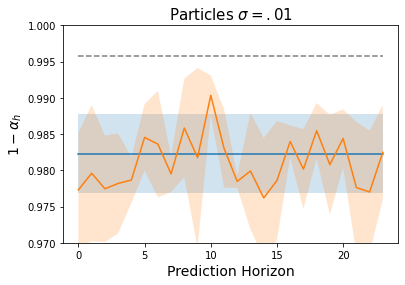
\includegraphics[width=\linewidth]{copula/figs/alphas/particle1.png}
  \label{fig:alpha-p1}
\end{subfigure}%
\begin{subfigure}{.45\textwidth}
  \centering
  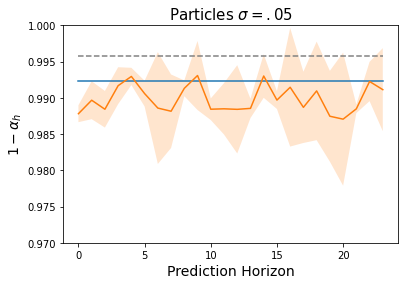
\includegraphics[width=\linewidth]{copula/figs/alphas/particle5.png}
  \label{fig:alpha-p2}
\end{subfigure}\\
\begin{subfigure}{.45\textwidth}
  \centering
  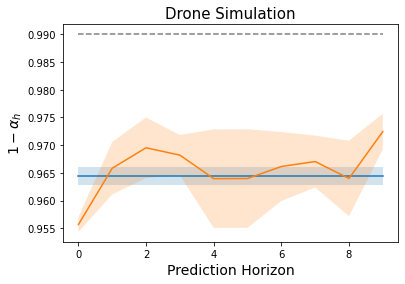
\includegraphics[width=\linewidth]{copula/figs/alphas/drone.png}
  \label{fig:alpha-drone}
\end{subfigure}%
\begin{subfigure}{.45\textwidth}
  \centering
  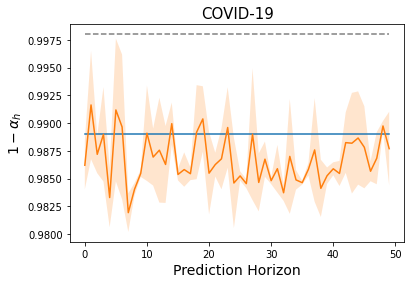
\includegraphics[width=\linewidth]{copula/figs/alphas/covid.png}
  \label{fig:alpha-covid}
\end{subfigure} \\
\begin{subfigure}{.46\textwidth}
  \centering
  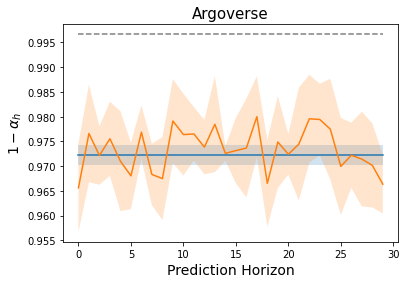
\includegraphics[width=\linewidth]{copula/figs/alphas/argo.png}
  \label{fig:alpha-argo}
\end{subfigure}
\begin{subfigure}{.45\textwidth}
  \centering
  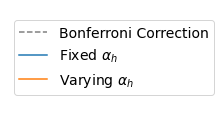
\includegraphics[width=0.6\linewidth]{copula/figs/alphas/labs.png}
  \label{fig:label}
\end{subfigure}
\caption{Comparison between dichotomy search for fixed $\alpha_h$ values (blue) and stochastic gradient search for varying $\alpha_h$ (blue) through timesteps. Shaded regions are the standard deviation of the values over 3 runs.} 
\label{fig:alpha}
\end{figure*}

\clearpage

\edit{
\subsection{Comparison to additional Baselines}}

We include a comparison to two additional simple UQ baselines on the particle simulation dataset. 

\textbf{L2-Conformal.} L2-Conformal uses the same underlying RNN forecaster as CF-RNN and Copula RNN.  We use that nonconformity score of the vector norm of all timesteps concatenated together $\| \hat{\textbf{y}}_{t+1:t+k} -\textbf{y}_{t+1:t+k} \|$ to perform ICP. As there are no analytic way to represent a $k \times d_y$-dimensional uncertainty region on 2-D space, we calculate the area and plot the region for L2 Conformal baseline with the maximum deviation at each timestep such that the vector norm still stays within range. 


\textbf{Direct Gaussian.} Direct Gaussian use the same model architecture and training hyperparameters, with the addition of a linear layer that outputs the variance for each timestep, and is optimized using negative log loss, a proper scoring rule for probabilistic forecasting. We obtain the area by analytically calculating the 90\% confidence interval for each variable.

Results in Table \ref{tab:partilel2} shows that L2-conformal produces inefficient confidence area, and directly outputting variance under-covers test data. These results align with previous findings and motivates our method, which is both more calibrated and sharper compared to these  baselines. We show a visualization in Figure \ref{fig:l2vis} to illustrate the different properties of the methods qualitatively.


\begin{table*}[h]
\centering
\begin{tabular}{ c | c c  | c c  |  } 
 \toprule
  & \multicolumn{2}{c}{Particle  ($\sigma=.01$)} & \multicolumn{2}{c}{Particle  ($\sigma=.05$)}\\
 \midrule
  Method & Coverage  (90\%) & Area  $\downarrow$ & Coverage  (90\%) & Area  $\downarrow$ \\
\midrule  
 L2-Conformal & $88.5 \pm 0.4$ & $7.21 \pm 0.35$  &  $89.7 \pm 0.6$  & $7.21 \pm 0.35$ \\
 Direct Gaussian & $11.9 \pm 0.09$ & $0.07 \pm 0.31$  & $0.0 \pm 0.0$ & $0.08 \pm 0.02$ \\
 CF-RNN &  $97.0 \pm 2.3$ & $3.13 \pm 3.24$ &  $97.0 \pm 2.3$ &  $5.79 \pm 0.51$ \\
 Copula-RNN & $\textbf{91.5} \pm 2.1$ & $\textbf{1.06} \pm 0.36$ & $\textbf{90.3} \pm 0.7$ & $\textbf{4.50} \pm 0.07$ \\
\bottomrule
 \end{tabular}
 \caption{ Comparison with two additional baselines on the particle dataset. }
\label{tab:partilel2}
 \end{table*}
 
 
\begin{figure}[h]
\centering
\begin{subfigure}[b]{0.45\linewidth}
  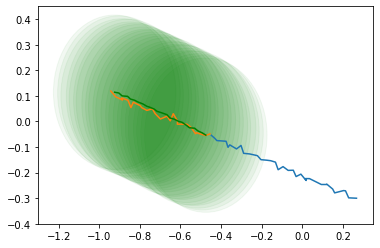
\includegraphics[width=\linewidth]{copula/figs/baselines2/l2.png}
  \caption{L2 Conformal}
  \label{fig:r1}
\end{subfigure}%
\begin{subfigure}[b]{0.45\linewidth}
  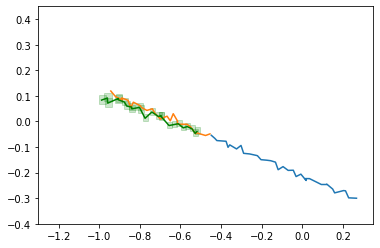
\includegraphics[width=\linewidth]{copula/figs/baselines2/gaussian.png}
  \caption{Direct RNN Gaussian}
  \label{fig:r2}
\end{subfigure}
\begin{subfigure}[b]{0.45\linewidth}
  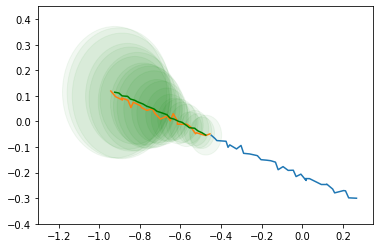
\includegraphics[width=\linewidth]{copula/figs/baselines2/cfrnn.png}
  \caption{CF-RNN}
  \label{fig:r3}
\end{subfigure}
\begin{subfigure}[b]{0.45\linewidth}
  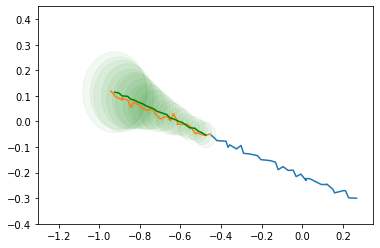
\includegraphics[width=\linewidth]{copula/figs/baselines2/copula.png}
  \caption{Copula-RNN}
  \label{fig:r4}
\end{subfigure}
\caption{ Visualization of on a sample from the Particle dataset's test set.  }
\label{fig:l2vis}
\end{figure}

% \begin{table*}[h]
% \centering
% \begin{tabular}{ c | c c   c c  |  } 
%  \toprule
%  Method & Coverage (90\%) & Area $\downarrow$ \\
% \midrule 
%  L2-Conformal & $88.5 \pm 0.4$ & $7.21 \pm 0.35$ \\
%  Direct Gaussian& $11.9 \pm 0.09$ & $0.07 \pm 0.31$ \\
%  CF-RNN &  $97.0 \pm 2.3$ & $3.13 \pm 3.24$ \\
%  Copula-RNN & $\textbf{91.5} \pm 2.1$ & $\textbf{1.06} \pm 0.36$ \\
% \bottomrule
%  \end{tabular}
%  \caption{ Particle dataset $\sigma = 0.01$, with confidence $1-\alpha = 0.9$  }
% \label{tab:partile1l2}
%  \end{table*}
 
 
 


\chapter{Conformal Prediction for Time-series Forecasting with Change Points}

% \documentclass{article} % For LaTeX2e

% \usepackage{hyperref}
% \usepackage{url}
% \usepackage{microtype}
% \usepackage{graphicx} %[dvipdfmx]
% \usepackage{caption}
% \usepackage{subcaption}
% \usepackage{booktabs} 
% \usepackage{bbm}% for professional tables
% \usepackage{hyperref}
% \usepackage{tikz}
% \usepackage{wrapfig}
% \usepackage{amsmath}
% \usepackage{amssymb}
% \usepackage{mathtools}
% \usepackage{wrapfig}
% \usepackage{amsthm}
% \usepackage{float}

% \newcommand{\theHalgorithm}{\arabic{algorithm}}

% \usepackage[ruled, lined, linesnumbered, commentsnumbered, longend]{algorithm2e}

% \usepackage{xcolor}
% \definecolor{mygray}{gray}{0.4}

% %%%%% NEW MATH DEFINITIONS %%%%%

\usepackage{hyperref}
\usepackage{url}
\usepackage{microtype}
\usepackage{graphicx} %[dvipdfmx]
\usepackage{booktabs} 
\usepackage{multirow}

\usepackage{bbm}% for professional tables
\usepackage{hyperref}
\usepackage{tikz}
\usepackage{wrapfig}
\usepackage{amssymb}
\usepackage{mathtools}
\usepackage{wrapfig}
\usepackage{float}

\usepackage{amsmath,amsfonts,bm, amsthm}
\usepackage[ruled, lined, linesnumbered, commentsnumbered, longend]{algorithm2e}
\usepackage[normalem]{ulem}
\newcommand{\stkout}[1]{\ifmmode\text{\sout{\ensuremath{#1}}}\else\sout{#1}\fi}


\usepackage{microtype}
\usepackage{balance}
\usepackage{enumitem}
\usepackage{hyperref}
\usepackage{url}
\usepackage{bbold}
\newtheorem*{claim}{Claim} 
\usepackage[margin=1em]{caption}
\usepackage{subcaption}

\AtBeginDocument{%
%\setlength{\abovecaptionskip}{0pt}% if captions above content
\setlength{\belowcaptionskip}{12pt}% if captions below content
}

\newcommand{\M}[1]{{\mathbf{#1}}} % matrix
\newcommand{\T}[1]{{\mathcal{#1}}} % tensor
\newcommand{\V}[1]{{\mathbf{#1}}} % vector
\newcommand{\real}{{\mathbb{R}}} % real
\captionsetup{format=plain}



%%%%%%%%%%%%%%%%%%%%%%%%%%%%%%%%
% THEOREMS
%%%%%%%%%%%%%%%%%%%%%%%%%%%%%%%%
% \theoremstyle{plain}
% \newtheorem{theorem}{Theorem}[section]
% \newtheorem{proposition}[theorem]{Proposition}
% \newtheorem{lemma}[theorem]{Lemma}
% \newtheorem{corollary}[theorem]{Corollary}
% \theoremstyle{definition}
% \newtheorem{definition}[theorem]{Definition}
% \newtheorem{assumption}{Assumption}
% \newtheorem*{theorem*}{Theorem}


\theoremstyle{definition}
\newtheorem{theorem}{Theorem}
\newtheorem*{theorem*}{Theorem} %restate theorems
\newtheorem*{proposition*}{Proposition} %restate proposition
\newtheorem{lemma}{Lemma}
%\newtheorem{proposition}{Proposition}[theorem]
%eventually change to above version
\newtheorem{proposition}[theorem]{Proposition} 
\newtheorem{corollary}{Corollary}[theorem]
\newtheorem{definition}{Definition}[section]
\newtheorem{assumption}{Assumption}[section]
\newtheorem{notation}[theorem]{Notation}
\newtheorem{remark}{Remark}[theorem]



% \newtheorem{theorem}{Theorem}
\newtheorem*{prop*}{Proposition}
\newcommand{\rhoreg}{\rho_{\mathrm{reg}}}
\newcommand{\rhoin}{\rho_{\mathrm{in}}}
\newcommand{\rhoout}{\rho_{\mathrm{out}}}
\newcommand{\Rot}{\mathrm{Rot}}
\newcommand{\SOtwo}{\mathrm{SO}(2)}
\newcommand{\SO}{\mathrm{SO}}
\newcommand{\tout}{t_{\mathrm{out}}}
\newcommand{\tin}{t_{\mathrm{in}}}
\newcommand{\N}{[1\!\!:\!\!N]}



%\theoremstyle{plain}
% \newtheorem{theorem}{Theorem}[section]
% \newtheorem{proposition}[theorem]{Proposition}
% \newtheorem{lemma}[theorem]{Lemma}
% \newtheorem{corollary}[theorem]{Corollary}
% \newtheorem{assumption}{Assumption}
% \theoremstyle{definition}
% \newtheorem{definition}[theorem]{Definition}
% \theoremstyle{remark}
% \newtheorem{remark}[theorem]{Remark}

% Mark sections of captions for referring to divisions of figures
\newcommand{\figleft}{{\em (Left)}}
\newcommand{\figcenter}{{\em (Center)}}
\newcommand{\figright}{{\em (Right)}}
\newcommand{\figtop}{{\em (Top)}}
\newcommand{\figbottom}{{\em (Bottom)}}
\newcommand{\captiona}{{\em (a)}}
\newcommand{\captionb}{{\em (b)}}
\newcommand{\captionc}{{\em (c)}}
\newcommand{\captiond}{{\em (d)}}

% Highlight a newly defined term
\newcommand{\newterm}[1]{{\bf #1}}


% Figure reference, lower-case.
\def\figref#1{figure~\ref{#1}}
% Figure reference, capital. For start of sentence
\def\Figref#1{Figure~\ref{#1}}
\def\twofigref#1#2{figures \ref{#1} and \ref{#2}}
\def\quadfigref#1#2#3#4{figures \ref{#1}, \ref{#2}, \ref{#3} and \ref{#4}}
% Section reference, lower-case.
\def\secref#1{section~\ref{#1}}
% Section reference, capital.
\def\Secref#1{Section~\ref{#1}}
% Reference to two sections.
\def\twosecrefs#1#2{sections \ref{#1} and \ref{#2}}
% Reference to three sections.
\def\secrefs#1#2#3{sections \ref{#1}, \ref{#2} and \ref{#3}}
% Reference to an equation, lower-case.
\def\eqref#1{eqn~\ref{#1}}
% Reference to an equation, upper case
\def\Eqref#1{Eqn~\ref{#1}}
% A raw reference to an equation---avoid using if possible
\def\plaineqref#1{\ref{#1}}
% Reference to a chapter, lower-case.
\def\chapref#1{chapter~\ref{#1}}
% Reference to an equation, upper case.
\def\Chapref#1{Chapter~\ref{#1}}
% Reference to a range of chapters
\def\rangechapref#1#2{chapters\ref{#1}--\ref{#2}}
% Reference to an algorithm, lower-case.
\def\algref#1{algorithm~\ref{#1}}
% Reference to an algorithm, upper case.
\def\Algref#1{Algorithm~\ref{#1}}
\def\twoalgref#1#2{algorithms \ref{#1} and \ref{#2}}
\def\Twoalgref#1#2{Algorithms \ref{#1} and \ref{#2}}
% Reference to a part, lower case
\def\partref#1{part~\ref{#1}}
% Reference to a part, upper case
\def\Partref#1{Part~\ref{#1}}
\def\twopartref#1#2{parts \ref{#1} and \ref{#2}}

\def\ceil#1{\lceil #1 \rceil}
\def\floor#1{\lfloor #1 \rfloor}
\def\1{\bm{1}}
\newcommand{\train}{\mathcal{D}}
\newcommand{\valid}{\mathcal{D_{\mathrm{valid}}}}
\newcommand{\test}{\mathcal{D_{\mathrm{test}}}}

\def\eps{{\epsilon}}


% Random variables
\def\reta{{\textnormal{$\eta$}}}
\def\ra{{\textnormal{a}}}
\def\rb{{\textnormal{b}}}
\def\rc{{\textnormal{c}}}
\def\rd{{\textnormal{d}}}
\def\re{{\textnormal{e}}}
\def\rf{{\textnormal{f}}}
\def\rg{{\textnormal{g}}}
\def\rh{{\textnormal{h}}}
\def\ri{{\textnormal{i}}}
\def\rj{{\textnormal{j}}}
\def\rk{{\textnormal{k}}}
\def\rl{{\textnormal{l}}}
% rm is already a command, just don't name any random variables m
\def\rn{{\textnormal{n}}}
\def\ro{{\textnormal{o}}}
\def\rp{{\textnormal{p}}}
\def\rq{{\textnormal{q}}}
\def\rr{{\textnormal{r}}}
\def\rs{{\textnormal{s}}}
\def\rt{{\textnormal{t}}}
\def\ru{{\textnormal{u}}}
\def\rv{{\textnormal{v}}}
%\def\rw{{\textnormal{w}}}
\def\rx{{\textnormal{x}}}
%\def\ry{{\textnormal{y}}}
\newcommand{\ry}[1] {{\color{magenta} [RY: #1] } }
\newcommand{\edit}[1] { #1 } 
\newcommand{\sofi}[1] {{\color{blue} [sophia: #1] }}
\newcommand{\plusminus}[1] { \scriptsize{$\pm$ #1}}
\def\rz{{\textnormal{z}}}
% Random vectors
\def\rvepsilon{{\mathbf{\epsilon}}}
\def\rvtheta{{\mathbf{\theta}}}
\def\rva{{\mathbf{a}}}
\def\rvb{{\mathbf{b}}}
\def\rvc{{\mathbf{c}}}
\def\rvd{{\mathbf{d}}}
\def\rve{{\mathbf{e}}}
\def\rvf{{\mathbf{f}}}
\def\rvg{{\mathbf{g}}}
\def\rvh{{\mathbf{h}}}
\def\rvu{{\mathbf{i}}}
\def\rvj{{\mathbf{j}}}
\def\rvk{{\mathbf{k}}}
\def\rvl{{\mathbf{l}}}
\def\rvm{{\mathbf{m}}}
\def\rvn{{\mathbf{n}}}
\def\rvo{{\mathbf{o}}}
\def\rvp{{\mathbf{p}}}
\def\rvq{{\mathbf{q}}}
\def\rvr{{\mathbf{r}}}
\def\rvs{{\mathbf{s}}}
\def\rvt{{\mathbf{t}}}
\def\rvu{{\mathbf{u}}}
\def\rvv{{\mathbf{v}}}
\def\rvw{{\mathbf{w}}}
\def\rvx{{\mathbf{x}}}
\def\rvy{{\mathbf{y}}}
\def\rvz{{\mathbf{z}}}

% Elements of random vectors
\def\erva{{\textnormal{a}}}
\def\ervb{{\textnormal{b}}}
\def\ervc{{\textnormal{c}}}
\def\ervd{{\textnormal{d}}}
\def\erve{{\textnormal{e}}}
\def\ervf{{\textnormal{f}}}
\def\ervg{{\textnormal{g}}}
\def\ervh{{\textnormal{h}}}
\def\ervi{{\textnormal{i}}}
\def\ervj{{\textnormal{j}}}
\def\ervk{{\textnormal{k}}}
\def\ervl{{\textnormal{l}}}
\def\ervm{{\textnormal{m}}}
\def\ervn{{\textnormal{n}}}
\def\ervo{{\textnormal{o}}}
\def\ervp{{\textnormal{p}}}
\def\ervq{{\textnormal{q}}}
\def\ervr{{\textnormal{r}}}
\def\ervs{{\textnormal{s}}}
\def\ervt{{\textnormal{t}}}
\def\ervu{{\textnormal{u}}}
\def\ervv{{\textnormal{v}}}
\def\ervw{{\textnormal{w}}}
\def\ervx{{\textnormal{x}}}
\def\ervy{{\textnormal{y}}}
\def\ervz{{\textnormal{z}}}

% Random matrices
\def\rmA{{\mathbf{A}}}
\def\rmB{{\mathbf{B}}}
\def\rmC{{\mathbf{C}}}
\def\rmD{{\mathbf{D}}}
\def\rmE{{\mathbf{E}}}
\def\rmF{{\mathbf{F}}}
\def\rmG{{\mathbf{G}}}
\def\rmH{{\mathbf{H}}}
\def\rmI{{\mathbf{I}}}
\def\rmJ{{\mathbf{J}}}
\def\rmK{{\mathbf{K}}}
\def\rmL{{\mathbf{L}}}
\def\rmM{{\mathbf{M}}}
\def\rmN{{\mathbf{N}}}
\def\rmO{{\mathbf{O}}}
\def\rmP{{\mathbf{P}}}
\def\rmQ{{\mathbf{Q}}}
\def\rmR{{\mathbf{R}}}
\def\rmS{{\mathbf{S}}}
\def\rmT{{\mathbf{T}}}
\def\rmU{{\mathbf{U}}}
\def\rmV{{\mathbf{V}}}
\def\rmW{{\mathbf{W}}}
\def\rmX{{\mathbf{X}}}
\def\rmY{{\mathbf{Y}}}
\def\rmZ{{\mathbf{Z}}}

% Elements of random matrices
\def\ermA{{\textnormal{A}}}
\def\ermB{{\textnormal{B}}}
\def\ermC{{\textnormal{C}}}
\def\ermD{{\textnormal{D}}}
\def\ermE{{\textnormal{E}}}
\def\ermF{{\textnormal{F}}}
\def\ermG{{\textnormal{G}}}
\def\ermH{{\textnormal{H}}}
\def\ermI{{\textnormal{I}}}
\def\ermJ{{\textnormal{J}}}
\def\ermK{{\textnormal{K}}}
\def\ermL{{\textnormal{L}}}
\def\ermM{{\textnormal{M}}}
\def\ermN{{\textnormal{N}}}
\def\ermO{{\textnormal{O}}}
\def\ermP{{\textnormal{P}}}
\def\ermQ{{\textnormal{Q}}}
\def\ermR{{\textnormal{R}}}
\def\ermS{{\textnormal{S}}}
\def\ermT{{\textnormal{T}}}
\def\ermU{{\textnormal{U}}}
\def\ermV{{\textnormal{V}}}
\def\ermW{{\textnormal{W}}}
\def\ermX{{\textnormal{X}}}
\def\ermY{{\textnormal{Y}}}
\def\ermZ{{\textnormal{Z}}}

% Vectors
\def\vzero{{\bm{0}}}
\def\vone{{\bm{1}}}
\def\vmu{{\bm{\mu}}}
\def\vtheta{{\bm{\theta}}}
\def\va{{\bm{a}}}
\def\vb{{\bm{b}}}
\def\vc{{\bm{c}}}
\def\vd{{\bm{d}}}
\def\ve{{\bm{e}}}
\def\vf{{\bm{f}}}
\def\vg{{\bm{g}}}
\def\vh{{\bm{h}}}
\def\vi{{\bm{i}}}
\def\vj{{\bm{j}}}
\def\vk{{\bm{k}}}
\def\vl{{\bm{l}}}
\def\vm{{\bm{m}}}
\def\vn{{\bm{n}}}
\def\vo{{\bm{o}}}
\def\vp{{\bm{p}}}
\def\vq{{\bm{q}}}
\def\vr{{\bm{r}}}
\def\vs{{\bm{s}}}
\def\vt{{\bm{t}}}
\def\vu{{\bm{u}}}
\def\vv{{\bm{v}}}
\def\vw{{\bm{w}}}
\def\vx{{\bm{x}}}
\def\vy{{\bm{y}}}
\def\vz{{\bm{z}}}

% Elements of vectors
\def\evalpha{{\alpha}}
\def\evbeta{{\beta}}
\def\evepsilon{{\epsilon}}
\def\evlambda{{\lambda}}
\def\evomega{{\omega}}
\def\evmu{{\mu}}
\def\evpsi{{\psi}}
\def\evsigma{{\sigma}}
\def\evtheta{{\theta}}
\def\eva{{a}}
\def\evb{{b}}
\def\evc{{c}}
\def\evd{{d}}
\def\eve{{e}}
\def\evf{{f}}
\def\evg{{g}}
\def\evh{{h}}
\def\evi{{i}}
\def\evj{{j}}
\def\evk{{k}}
\def\evl{{l}}
\def\evm{{m}}
\def\evn{{n}}
\def\evo{{o}}
\def\evp{{p}}
\def\evq{{q}}
\def\evr{{r}}
\def\evs{{s}}
\def\evt{{t}}
\def\evu{{u}}
\def\evv{{v}}
\def\evw{{w}}
\def\evx{{x}}
\def\evy{{y}}
\def\evz{{z}}

% Matrix
\def\mA{{\bm{A}}}
\def\mB{{\bm{B}}}
\def\mC{{\bm{C}}}
\def\mD{{\bm{D}}}
\def\mE{{\bm{E}}}
\def\mF{{\bm{F}}}
\def\mG{{\bm{G}}}
\def\mH{{\bm{H}}}
\def\mI{{\bm{I}}}
\def\mJ{{\bm{J}}}
\def\mK{{\bm{K}}}
\def\mL{{\bm{L}}}
\def\mM{{\bm{M}}}
\def\mN{{\bm{N}}}
\def\mO{{\bm{O}}}
\def\mP{{\bm{P}}}
\def\mQ{{\bm{Q}}}
\def\mR{{\bm{R}}}
\def\mS{{\bm{S}}}
\def\mT{{\bm{T}}}
\def\mU{{\bm{U}}}
\def\mV{{\bm{V}}}
\def\mW{{\bm{W}}}
\def\mX{{\bm{X}}}
\def\mY{{\bm{Y}}}
\def\mZ{{\bm{Z}}}
\def\mBeta{{\bm{\beta}}}
\def\mPhi{{\bm{\Phi}}}
\def\mLambda{{\bm{\Lambda}}}
\def\mSigma{{\bm{\Sigma}}}

% Tensor
\DeclareMathAlphabet{\mathsfit}{\encodingdefault}{\sfdefault}{m}{sl}
\SetMathAlphabet{\mathsfit}{bold}{\encodingdefault}{\sfdefault}{bx}{n}
\newcommand{\tens}[1]{\bm{\mathsfit{#1}}}
\def\tA{{\tens{A}}}
\def\tB{{\tens{B}}}
\def\tC{{\tens{C}}}
\def\tD{{\tens{D}}}
\def\tE{{\tens{E}}}
\def\tF{{\tens{F}}}
\def\tG{{\tens{G}}}
\def\tH{{\tens{H}}}
\def\tI{{\tens{I}}}
\def\tJ{{\tens{J}}}
\def\tK{{\tens{K}}}
\def\tL{{\tens{L}}}
\def\tM{{\tens{M}}}
\def\tN{{\tens{N}}}
\def\tO{{\tens{O}}}
\def\tP{{\tens{P}}}
\def\tQ{{\tens{Q}}}
\def\tR{{\tens{R}}}
\def\tS{{\tens{S}}}
\def\tT{{\tens{T}}}
\def\tU{{\tens{U}}}
\def\tV{{\tens{V}}}
\def\tW{{\tens{W}}}
\def\tX{{\tens{X}}}
\def\tY{{\tens{Y}}}
\def\tZ{{\tens{Z}}}


% Graph
\def\gA{{\mathcal{A}}}
\def\gB{{\mathcal{B}}}
\def\gC{{\mathcal{C}}}
\def\gD{{\mathcal{D}}}
\def\gE{{\mathcal{E}}}
\def\gF{{\mathcal{F}}}
\def\gG{{\mathcal{G}}}
\def\gH{{\mathcal{H}}}
\def\gI{{\mathcal{I}}}
\def\gJ{{\mathcal{J}}}
\def\gK{{\mathcal{K}}}
\def\gL{{\mathcal{L}}}
\def\gM{{\mathcal{M}}}
\def\gN{{\mathcal{N}}}
\def\gO{{\mathcal{O}}}
\def\gP{{\mathcal{P}}}
\def\gQ{{\mathcal{Q}}}
\def\gR{{\mathcal{R}}}
\def\gS{{\mathcal{S}}}
\def\gT{{\mathcal{T}}}
\def\gU{{\mathcal{U}}}
\def\gV{{\mathcal{V}}}
\def\gW{{\mathcal{W}}}
\def\gX{{\mathcal{X}}}
\def\gY{{\mathcal{Y}}}
\def\gZ{{\mathcal{Z}}}

% Sets
\def\sA{{\mathbb{A}}}
\def\sB{{\mathbb{B}}}
\def\sC{{\mathbb{C}}}
\def\sD{{\mathbb{D}}}
% Don't use a set called E, because this would be the same as our symbol
% for expectation.
\def\sF{{\mathbb{F}}}
\def\sG{{\mathbb{G}}}
\def\sH{{\mathbb{H}}}
\def\sI{{\mathbb{I}}}
\def\sJ{{\mathbb{J}}}
\def\sK{{\mathbb{K}}}
\def\sL{{\mathbb{L}}}
\def\sM{{\mathbb{M}}}
\def\sN{{\mathbb{N}}}
\def\sO{{\mathbb{O}}}
\def\Prob{{\mathbb{P}}}
\def\prob{{\mathbb{P}}}
\def\sQ{{\mathbb{Q}}}
\def\sR{{\mathbb{R}}}
\def\sS{{\mathbb{S}}}
\def\sT{{\mathbb{T}}}
\def\sU{{\mathbb{U}}}
\def\sV{{\mathbb{V}}}
\def\sW{{\mathbb{W}}}
\def\sX{{\mathbb{X}}}
\def\sY{{\mathbb{Y}}}
\def\sZ{{\mathbb{Z}}}

% Entries of a matrix
\def\emLambda{{\Lambda}}
\def\emA{{A}}
\def\emB{{B}}
\def\emC{{C}}
\def\emD{{D}}
\def\emE{{E}}
\def\emF{{F}}
\def\emG{{G}}
\def\emH{{H}}
\def\emI{{I}}
\def\emJ{{J}}
\def\emK{{K}}
\def\emL{{L}}
\def\emM{{M}}
\def\emN{{N}}
\def\emO{{O}}
\def\emP{{P}}
\def\emQ{{Q}}
\def\emR{{R}}
\def\emS{{S}}
\def\emT{{T}}
\def\emU{{U}}
\def\emV{{V}}
\def\emW{{W}}
\def\emX{{X}}
\def\emY{{Y}}
\def\emZ{{Z}}
\def\emSigma{{\Sigma}}

% entries of a tensor
% Same font as tensor, without \bm wrapper
\newcommand{\etens}[1]{\mathsfit{#1}}
\def\etLambda{{\etens{\Lambda}}}
\def\etA{{\etens{A}}}
\def\etB{{\etens{B}}}
\def\etC{{\etens{C}}}
\def\etD{{\etens{D}}}
\def\etE{{\etens{E}}}
\def\etF{{\etens{F}}}
\def\etG{{\etens{G}}}
\def\etH{{\etens{H}}}
\def\etI{{\etens{I}}}
\def\etJ{{\etens{J}}}
\def\etK{{\etens{K}}}
\def\etL{{\etens{L}}}
\def\etM{{\etens{M}}}
\def\etN{{\etens{N}}}
\def\etO{{\etens{O}}}
\def\etP{{\etens{P}}}
\def\etQ{{\etens{Q}}}
\def\etR{{\etens{R}}}
\def\etS{{\etens{S}}}
\def\etT{{\etens{T}}}
\def\etU{{\etens{U}}}
\def\etV{{\etens{V}}}
\def\etW{{\etens{W}}}
\def\etX{{\etens{X}}}
\def\etY{{\etens{Y}}}
\def\etZ{{\etens{Z}}}

% The true underlying data generating distribution
\newcommand{\pdata}{p_{\rm{data}}}
% The empirical distribution defined by the training set
\newcommand{\ptrain}{\hat{p}_{\rm{data}}}
\newcommand{\Ptrain}{\hat{P}_{\rm{data}}}
% The model distribution
\newcommand{\pmodel}{p_{\rm{model}}}
\newcommand{\Pmodel}{P_{\rm{model}}}
\newcommand{\ptildemodel}{\tilde{p}_{\rm{model}}}
% Stochastic autoencoder distributions
\newcommand{\pencode}{p_{\rm{encoder}}}
\newcommand{\pdecode}{p_{\rm{decoder}}}
\newcommand{\precons}{p_{\rm{reconstruct}}}

\newcommand{\laplace}{\mathrm{Laplace}} % Laplace distribution

\newcommand{\E}{\mathbb{E}}
\newcommand{\Ls}{\mathcal{L}}
\newcommand{\R}{\mathbb{R}}
\newcommand{\emp}{\tilde{p}}
\newcommand{\lr}{\alpha}
\newcommand{\reg}{\lambda}
\newcommand{\rect}{\mathrm{rectifier}}
\newcommand{\softmax}{\mathrm{softmax}}
\newcommand{\sigmoid}{\sigma}
\newcommand{\softplus}{\zeta}
\newcommand{\KL}{D_{\mathrm{KL}}}
\newcommand{\Var}{\mathrm{Var}}
\newcommand{\standarderror}{\mathrm{SE}}
\newcommand{\Cov}{\mathrm{Cov}}
% Wolfram Mathworld says $L^2$ is for function spaces and $\ell^2$ is for vectors
% But then they seem to use $L^2$ for vectors throughout the site, and so does
% wikipedia.
\newcommand{\normlzero}{L^0}
\newcommand{\normlone}{L^1}
\newcommand{\normltwo}{L^2}
\newcommand{\normlp}{L^p}
\newcommand{\normmax}{L^\infty}

\newcommand{\parents}{Pa} % See usage in notation.tex. Chosen to match Daphne's book.

\DeclareMathOperator*{\argmax}{arg\,max}
\DeclareMathOperator*{\argmin}{arg\,min}

\DeclareMathOperator{\sign}{sign}
\DeclareMathOperator{\Tr}{Tr}
\let\ab\allowbreak

\newcommand{\Dcal}{\mathcal{D}_{cal}}
\newcommand{\Dtrain}{\mathcal{D}_{train}}
\newcommand{\Dtest}{\mathcal{D}_{test}}
\newcommand{\Dcalone}{\mathcal{D}_{cal-1}}
\newcommand{\Dcaltwo}{\mathcal{D}_{cal-2}}
\newcommand{\infinityvec}{\{ \boldsymbol{\infty} \}}




% \newcommand{\fix}{\marginpar{FIX}}
% \newcommand{\new}{\marginpar{NEW}}
% \newcommand{\ryedit}[1]{{\color{magenta} #1}}
% \newcommand{\ryu}[1]{\ryedit{[RY: #1]}}


% \usepackage[final]{neurips_2025}

% to compile a preprint version, e.g., for submission to arXiv, add add the
% [preprint] option:
%     \usepackage[preprint]{neurips_2024}


% to compile a camera-ready version, add the [final] option, e.g.:
%     \usepackage[final]{neurips_2024}


% If accepted, instead use the following line for the camera-ready submission:
%\usepackage[accepted]{icml2024}


% \title{Conformal Prediction for Time-series Forecasting with Change Points}

% \author{%
% Sophia Sun, Rose Yu \\
%  Computer Science and Engineering\\
%  University of California, San Diego\\
%  % \texttt{hippo@cs.cranberry-lemon.edu}
% %  \And
% %   Rose Yu \\
% % Computer Science and Engineering\\
% %  University of California, San Diego\\
%   }

% \begin{document}


% \maketitle

% \begin{abstract} Conformal prediction has been explored as a general and efficient way to provide uncertainty quantification for time series. However, current methods struggle to handle time series data with change points — sudden shifts in the underlying data-generating process. In this paper, we propose a novel Conformal Prediction for Time-series with Change points (CPTC) algorithm, addressing this gap by integrating a model to predict the underlying state with online conformal prediction to model uncertainties in non-stationary time series. We prove CPTC's validity and improved adaptivity in the time series setting under minimum assumptions, and demonstrate CPTC's practical effectiveness on 6 synthetic and real-world datasets, showing improved validity and adaptivity compared to state-of-the-art baselines.
% \end{abstract}

\section{Introduction}
%Time series forecasting plays a crucial role in numerous applications, including energy, healthcare, and climate modeling, where predicting future values based on historical data can drive critical decisions. In the decision process, Uncertainty Quantification (UQ) plays a pivotal role as it allows us to estimate the confidence of our predictions, and reason about potential outcomes in a systematic manner. 


Uncertainty Quantification (UQ) is a key building block of reliable machine learning systems. Conformal prediction (CP) is a popular distribution-free UQ method that provides finite sample coverage guarantees without placing assumptions on the underlying data generating process \citep{vovk2005algorithmic, lei2018distribution}. Because of its simplicity and generality, conformal prediction has seen wide adoption in many tasks, ranging from  healthcare \cite{angelopoulos2022conformal},  robotics \cite{lindemann2023safe}, to validating the factuality of  generative models \cite{cherian2024large}.

Existing CP algorithms for time series forecasting mostly adopt an online learning framework \cite{gibbs2024conformal, angelopoulos2024pid}, where the prediction interval adapts to distribution changes in data \textit{reactively}. The online CP algorithms achieve a asymptotic marginal coverage guarantee (the miscoverage rate converges to a specified fraction as the time horizon goes to infinity). As a result, the algorithms inevitably exhibit miscoverage when distribution shifts occur, and then have to over- or under-cover in later timesteps to compensate. This behavior is evident in the ACI and CP baselines in Figure \ref{fig:cov}. This is undesirable in practice as these under-covered periods may incur a lot of risk.

This paper builds upon the observation that in real-world scenarios, distribution shifts in time-series are often \textit{predictable}. Take for example the task of forecasting electricity demands: we know that the hidden dynamics may differ between day and night, or during weekdays and weekends. The same logic applies to traffic forecasting and product demand forecasting, where there are patterns in the shifts between ``surge times" and ``normal times". In this work, we study time series data that exhibit this type of abrupt shifts, or change points, in the underlying generative process. 

State Space Models (SSMs) \citep{kalman1960new, aoki2013state} are a powerful tool for modeling time series data, as they provide a structured framework to capture the underlying temporal dependencies through latent states. In particular, Switching Dynamical Systems (SDS) \citep{ackerson1970state} is a type of SSM with an additional set of latent variables (known as \textit{switches}) that represent the operating mode active at the current timestep. SDS introduces the inductive biases that allow SSMs to switch between a discrete set of dynamics, which can be learned from training data. It is shown to be a flexible, robust, and interpretable representation of time series with varying dynamics exhibiting change points \citep{ansari2021deep, chen2022learning}. SDS is deployed not only for energy \cite{karakatsani2008intra, song2014short, fan2008machine} and traffic \cite{yu2004switching, cetin2006short} forecasting as  examples given above, but also on a wide range of applications including neuroscience \cite{glaser2020recurrent, rabinovich2006dynamical, kato2015global}, engineering \cite{strachan2011measuring,wang2007actively}, and sports analytics \cite{yamamoto2018switching}, all would benefit from robust and calibrated uncertainty quantification. 

Our code is open source at \url{https://github.com/huiwenn/CPTC}. Our contributions are:

%\begin{wrapfigure}{r}{0.5\textwidth}
\begin{figure}[tb]
    \vspace{-1em}
    \centering
    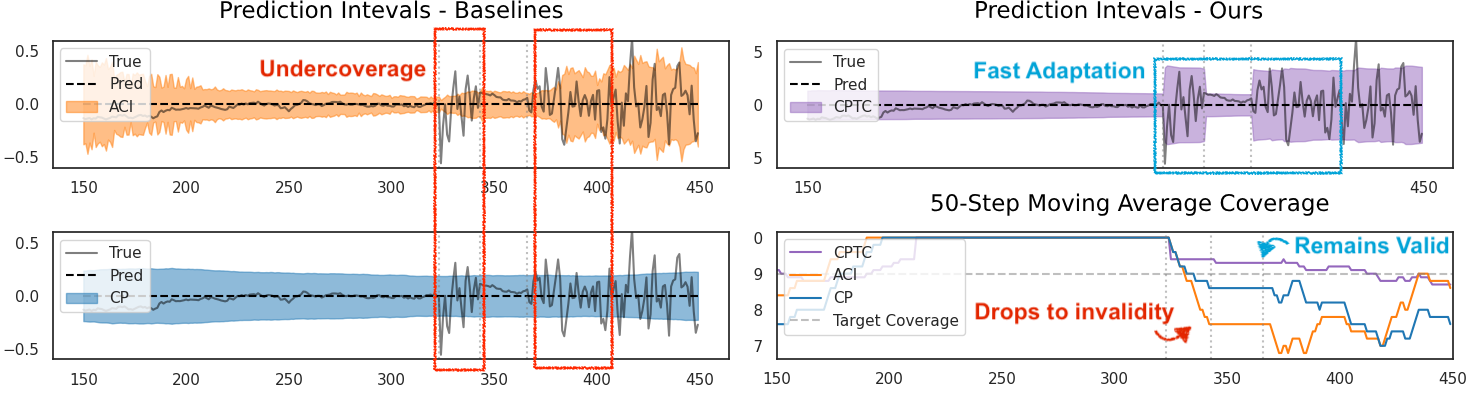
\includegraphics[width=1.01\linewidth]{changepoints/figs/ex/ex_zoom.png}
    \caption{Comparison of the prediction intervals obtained by our algorithm CPTC (purple) against online conformal prediction baselines on synthetic data. The vertical dashed line marks the distribution shifts; ideal behavior is consistent coverage at the horizontal dashed line in the final panel. Bottom right panel shows that CPTC achieves fast adaptation and remains valid when change points occur.}
    \label{fig:cov}
    \vspace{-1em}

\end{figure}
%    \vspace{-2.0em}
%\end{wrapfigure}

%
\vspace{-0.5em}
\begin{itemize}
    \item We propose a new algorithm \textbf{C}onformal \textbf{P}rediction for \textbf{T}ime series with \textbf{C}hange points (CPTC) that utilizes state transition predictions to improve uncertainty quantification for time-series forecasts. Leveraging properties of a SDS model, CPTC consolidates multiple future forecasts to adaptively adjust its prediction intervals when underlying dynamics shift.
    \item We prove that CPTC achieves asymptotic valid coverage, \textit{without assumptions} on the data generation process or state transition model accuracy. When predicted state transitions align well with distribution shifts, CPTC can anticipate uncertainty and adapt faster.
    \item We show strong empirical results on 3 synthetic and 3 real-world datasets. Compared to online conformal prediction baselines, CPTC achieves more robust coverage with comparable prediction intervals sharpness (example in Figure \ref{fig:cov}), and is computationally light.%Compared to  CP algorithms leveraging temporal structures (SPCI \cite{xu2023sequential} and HopCPT \cite{auer2023hopcpt}), CPTC is computationally lighter and more data-efficient.
\end{itemize}

%Conformal prediction produces a $(1-\alpha)$-prediction interval $\Gamma^{1-\alpha}$ for a random variable $y$, which is \textit{valid} if it contains $y$'s true value with high probability:  
%$
%\Prob[y \in \Gamma^{1-\alpha}] \geq 1-\alpha.
%$
%Note that one can make the prediction interval infinitely large to satisfy validity. But for the prediction interval to be useful, we also want to minimize its area while remaining valid; this is known as the \textit{sharpness} of the region. 


% \begin{figure}[h]
%     \centering
%     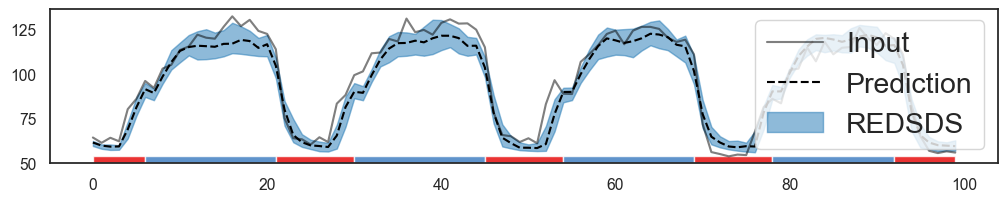
\includegraphics[width=0.9\linewidth]{changepoints/figs/e-prob.png}
%     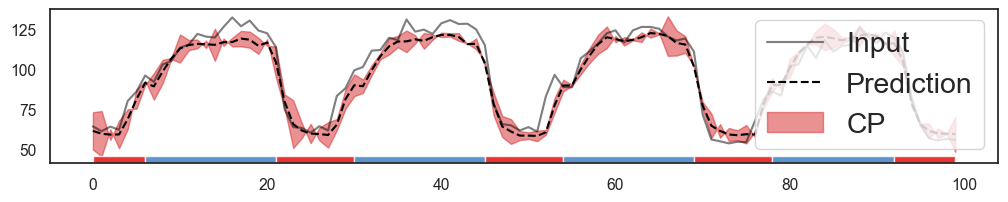
\includegraphics[width=0.9\linewidth]{changepoints/figs/e-cp.png}
%         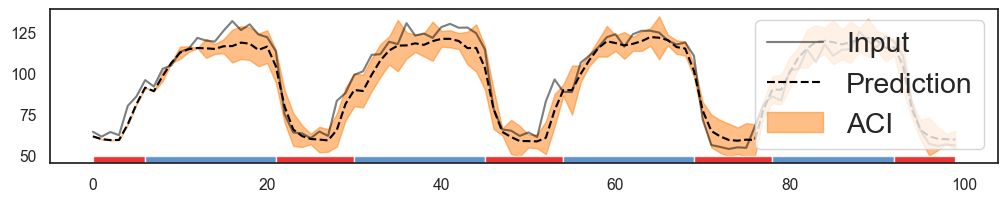
\includegraphics[width=0.9\linewidth]{changepoints/figs/e-aci.png}
%     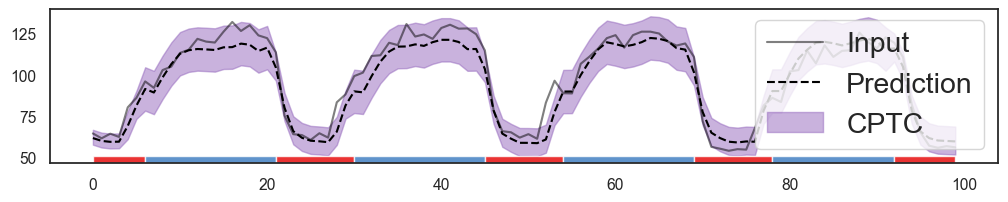
\includegraphics[width=0.9\linewidth]{changepoints/figs/e-ours.png}
%     \caption{Demonstration of uncertainty quantification baselines on hourly electricity demand. Our method (green regions) adapts to different levels of volatility between day and night and whereby achieves more stable coverage over time, whereas ACI (yellow) over-covers during red phases and under-covers during blue.}
%     \label{fig:demonstration}
% \end{figure}


\section{Related Work}
%\vspace{-0.5em}

% \paragraph{Time series forecasting with switching dynamical systems}  State-space models (Fraccaro et al., 2017; Rangapuram
% et al., 2018; de Bézenac et al., 2020; Tang & Matteson, 2021; Klushyn et al., 2021) and recurrent neural
% networks (Salinas et al., 2019; 2020; Rasul et al., 2021b;a) are among the most popular choices to model
% temporal dependencies in time series. 

% However, for these models to generalize and adapt to new changes in the future, it is
% critical to have appropriate inductive biases built into the model. A common approach is to allow state-space models to switch between a discrete set of dynamics, which can be learned from training data.

\vspace{-0.5em}
\paragraph{Probabilistic Forecasting for Time-Series with Change Points.} %Deep learning has enabled substantial advances in time series forecasting. in order to represent the inherent stochasticity of real-world time series data. 
%Probabilistic forecasting methods model distributions over possible outcomes \citep{benidis2022deep}, and have been used widely to build predicting intervals.
%Bayesian Neural Networks (BNN) for uncertainty quantification (UQ) of spatiotemporal forecasts. In practice, Bayesian UQ can be computationally expensive and difficult to optimize, especially for larger networks \citep{lakshminarayanan2017simple, zadrozny2001obtaining}. Therefore, UQ for deep neural network time series forecasts often adopts approximate Bayesian inference such as MC-dropout \citep{gal2016theoretically, gal2017concrete}. Neural process models use neural network to parameterize a stochastic process \citep{garnelo2018conditional,garnelo2018neural, sun2024data}. 
%Method such as (approximate) Bayesian Neural Networks  \citep{wang2019deep, wu2021quantifying, gal2017concrete} and neural process models \citep{garnelo2018conditional, sun2024data} use neural networks to parametrize traditional probabilistic frameworks for time-series forecasting. Other deep-learning models such as DeepAR \citep{salinas2020deepar}, PatchTST \citep{nie2023patchtst}, and Temporal Fusion Transformer \citep{lim2021temporal} directly generate probabilistic forecasts by training the model with pinball loss. 

Probabilistic forecasting has become central to modern time-series analysis by modeling a distribution over future outcomes rather than a single-point forecast \citep{benidis2022deep}. Classic approaches often adopt Bayesian or approximate Bayesian strategies for uncertainty quantification: for instance, Bayesian Neural Networks (BNNs) \citep{wang2019deep, wu2021quantifying, gal2017concrete} or neural process models \citep{garnelo2018conditional, sun2024data} use neural networks to parameterize the underlying stochastic process. Other methods, such as DeepAR \citep{salinas2020deepar}, PatchTST \citep{nie2023patchtst}, or Temporal Fusion Transformer \citep{lim2021temporal}, generate probabilistic forecasts directly by minimizing a pinball loss (i.e., quantile loss), thereby learning predictive distributions.

%\textit{Change points} refer to abrupt distribution shifts in observational time series data \citep{montanez2015inertial}. Detecting and segmenting change points has been studied extensively (see \cite{aminikhanghahi2017survey} for a recent survey), %\citep{adams2007bayesian, agudelo2020bayesian, chiappa2010movement}, 
%whereas modeling time series with change points is typically approached with SSM, and in particular SDS. Recent works in SDS 
%mostly deploy variational inference \citep{johnson2016composing, ansari2021deep, liu2023graph}, using neural networks to parametrize the transition or emission distributions. \cite{sun2024online} studies UQ for change points but in the anomaly detection setting. % to improve flexibility and accelerate inference.

A key challenge arises when \textit{change points} occur - i.e., abrupt distribution shifts in the time series \citep{montanez2015inertial}. Change point detection and segmentation have been studied extensively (beyond our scope, see \citep{aminikhanghahi2017survey} for a recent survey). Modeling time series with change points typically features state-space models (SSM), and in particular switching dynamical systems (SDS) \citep{johnson2016composing, ansari2021deep, liu2023graph}. These SDS approaches use variational inference to fit neural parameterizations of transitions and emission distributions. However, existing probabilistic forecasters often lack strict calibration guarantees and can be overconfident in practice \citep{lakshminarayanan2017simple}, and many require specialized architecture tuning for different tasks, limiting their applicability to real-world UQ challenges.


% Compared to ours and other CP approaches, the drawbacks of the aforementioned methods are: (1) they are not model-free, i.e. special designs of the predictive model and hyper-parameter tuning are required, and (2) they have no theoretical guarantee on calibration and often are overconfident in practice \citep{lakshminarayanan2017simple}.

%SDS models, most often represented as a graphical model, have seen a surge in using neural networks to parameterize transition and emission distributions \citep{johnson2016composing, ansari2021deep, liu2023graph}, to improve flexibility and fast inference. Bayesian and variational inference methods are used extensively in online change point detection \citep{adams2007bayesian, agudelo2020bayesian} and segmentation \citep{chiappa2010movement} as well. 

% Our work focuses on only discrete states, which come with the benefit of interpretability and scalability. Discrete SSMs have been used to address safety-critical distribution shifts, such as reasoning about occlusion in traffic scenes \cite{wei2024navigation}. 

%The challenge of these Bayesian, RNN-, or Transformer-based probabilistic models is that the forecasted probabilities are often uncalibrated or overconfident \citep{lakshminarayanan2017simple}, hence unsuitable for many practical tasks that require guarantees on the uncertainty estimates associated with the forecasts. 

%Frequentist UQ methods emphasize robustness against variations in the data. These approaches either rely on resampling the data or learning an interval bound to encompass the dataset. For time series forecasting UQ, approaches include ensemble methods such as bootstrap \citep{efron2016, bjrnn} and jackknife methods  \citep{jackknife+after, bjrnn}; interval prediction methods include interval regression through proper scoring rules \citep{kivaranovic2020adaptive, wu2021quantifying}, and quantile regression \citep{takeuchi2006nonparametric}, with many recent advances for time series UQ  \citep{tagasovska2019single, gasthaus2019probabilistic,park2022learning, kan2022multivariate}. Many of the frequentist methods produce asymptotically valid confidence regions and can be categorized as distribution-free UQ techniques as they are (1) agnostic to the underlying model and (2) agnostic to data distribution.

\vspace{-0.5em}
\paragraph{Conformal Prediction for time-series.} 
%Conformal prediction (CP), originally introduced in \cite{vovk2005algorithmic}, has become a popular UQ method because of its simplicity, generality,  coverage guarantee, and low computational cost; we refer readers to \cite{angelopoulos2021gentle} for a comprehensive introduction to CP. For time series prediction, \cite{Schaar2021conformaltime, sun2023copula, zhou2024heterogeneous} aims for joint coverage and formulates fixed-length time series problems as exchangeable multi-target forecasts. Enbpi \citep{xu2021conformal} and SPCI \citep{xu2023sequential} assume no change in system dynamics, but in the generating process of the noise or residual that causes uncertainty.  \cite{tibshirani2019conformal} adapts to \textit{known} covariance shift by weighting data using propensity scores. Although theoretically optimal, the algorithm does not apply to real-world problems where propensity scores are difficult to calculate. Adaptive conformal inference (ACI) \citep{gibbs2021adaptive} and its variants \citep{zaffran2022adaptive, gibbs2024conformal, angelopoulos2024pid} consider the online adversarial setting, where they guarantee target marginal coverage without any assumptions on the data generating process. 

Conformal prediction (CP) \citep{vovk2005algorithmic} has emerged as a leading framework for UQ due to its algorithmic simplicity, broad applicability, and finite-sample coverage guarantees; see \cite{angelopoulos2021gentle} for a comprehensive introduction. For time-series forecasting, some works focus on joint coverage over fixed-length horizons \citep{Schaar2021conformaltime, sun2023copula, zhou2024heterogeneous}; others assume stable underlying dynamics and adapt only to shifts in residual distributions \citep{xu2021conformal} . \cite{tibshirani2019conformal} uses known covariate shifts (by propensity weighting) to achieve theoretical coverage, but can fail in settings where the shift mechanism is unknown, which is typical for time series forecasting. \cite{hajihashemi2024multi} introduces a multi-model ensemble CP framework, optimizing model selection within a pool of experts for combined coverage.  CP has also been extended for change-point detection in time series via conformal martingales \citep{vovk2021retrain, volkhonskiy2017inductive}. 

Recent works on online conformal prediction develop online strategies that guarantee marginal coverage for adversarial or nonstationary data streams. ACI \citep{gibbs2021adaptive}, AgACI \citep{zaffran2022adaptive}, DtACI \citep{gibbs2024conformal}, and Conformal PID control \citep{angelopoulos2024pid}  leverage online optimization and have a "reaction" period when distribution shifts. Multivalid Prediction (MVP) \citep{bastani2022practical} provides group coverage guarantees and learns a calibration threshold online, although it can require longer calibration windows. Closer to our work, SPCI \citep{xu2023sequential} learns an autocorrelative estimation of the residual's quantiles through Quantile Random Forest; whereas HopCPT \citep{auer2023hopcpt} condition their conformal interval on similar parts of the time series using a Modern Hopfield Network. The drawback of these two methods is that the regression models are trained during inference time, which (1) requires a long cold start window to learn meaningful associations and (2) is computationally expensive. 
%
Our contribution is a CP algorithm that is computationally light during inference time, and can leverage state prediction capabilities within the SDS model to anticipate and adapt quickly to distribution changes.


%Closest to our work are (1) SPCI \citep{xu2023sequential} learns a time-adaptive estimation of residual quantiles over time, upon leveraging the temporal dependency among them. However, SPCI's theoretical results rely on the properties of a specific quantile learning algorithm, which does not always apply to the time series of interest.(2) Multivalid Prediction (MVP) \citep{bastani2022practical} which guarantees group conditioned coverage in the online adversarial setting. MVP requires a longer sequence as the calibration threshold is learned online. Our work brings their theoretical results into a more practical setting. Our approach also achieves group conditional coverage, which builds upon results from SPCI and MVP. A similar result can be found in \cite{zhou2024heterogeneous} with the name approximate conditional coverage, although only empirical evidence is shown.

%Most relevant to our work is the recent endeavor in generalizing CP to time-series forecasting. \cite{Schaar2021conformaltime} and \cite{sun2023copula} studies . In the case of distribution shifts, ACI \citep{gibbs2021adaptive} and EnbPI \citep{xu2021conformal} developed CP algorithms that relax the exchangeability assumption while maintaining asymptotic validity via online learning (former) and ensembling (later); \cite{zaffran2022adaptive} further improves online adaptation.  \cite{sousa2022general} combines EnbPI with conformal quantile regression \citep{romano2019conformalized} to model heteroscedastic time series. 








\section{Background}


\subsection{Conformal Prediction}
%\sofi{highlight the difference between conformal and split, differenciation}

We briefly review the algorithm and guarantees for conformal prediction, and refer readers to~\cite{angelopoulos2021gentle} for a thorough introduction. In this paper CP refers to \textit{split conformal prediction} (we consider full conformal prediction out of scope, because its computationally complexity renders it nonviable for deep learning settings). The goal of conformal prediction is to produce a \textit{valid} prediction interval (Def.~\ref{def:validity}) for any underlying prediction model.
%
\begin{definition}[Validity]
Given a new data point $(x,y)$, where $y$ is the prediction target and $x$ is the covariates,  and a desired confidence $1-\alpha \in (0,1)$, the prediction interval $\Gamma^{1-\alpha}(x)$ is a subset of $\mathcal{Y}$ containing probable outputs given $x$. The region $\Gamma^{1-\alpha}$ is valid if
%
\begin{equation}\label{eq:coverage}
P (y \in \Gamma^{1-\alpha}(x)) \geq 1-\alpha
 \end{equation}
\label{def:validity}
\end{definition}
%
\vspace{-2em}
Let $\mathcal{D} = \{ (x^i, y^i)\}_{i=1}^n$ be a dataset whose data points $(x^i, y^i)$ are sampled from a distribution on $ \mathcal{X} \times \mathcal{Y}$.  Conformal prediction splits the dataset into a proper training set $\Dtrain$ and a calibration set $\Dcal$. A prediction model $\hat{f}: \mathcal{X} \rightarrow  \mathcal{Y}$ is trained on $\Dtrain$. We use a \textit{nonconformity score} function $A: \mathcal{X} \times  \mathcal{Y} \rightarrow \R_{\geq 0}$ to quantify how well a data sample from calibration \textit{conforms} to the training dataset. Typically, we choose a metric of disagreement between the prediction and the true label as the non-conformity score, such as the Euclidean distance: 
%
\begin{equation}
 A(x,y) \stackrel{\text{e.g.}}{=} d(y,\hat{f}(x)) \stackrel{\text{e.g.}}{=} 
\|y - \hat{f}(x)\|_2 
\label{def:non-c}
\end{equation}
%
Let $\gS = \{A(x^i, y^i)\}_{(x^i, y^i) \in \Dcal}$ denote the set of nonconformity scores of all samples in the calibration set $\Dcal$. %We define a quantile function for nonconformity scores $\gS$ as:
%
During inference time given a new data  $x^{n+1}$, the conformal prediction interval is constructed as in \Eqref{eq:region}, where $Q$ is the empirical quantile function. 
%
\begin{equation}
    \Gamma^{1-\alpha}(x^{n+1}):=  \{ y : A(x^{n+1}, y) \leq Q^{1-\alpha}(\gS \cup \{\infty\})\}  
    \label{eq:region}
\end{equation}
%
% \begin{equation}
%     Q(1-\alpha, \gS) := \text{inf} \{s^*: (\frac{1}{|\gS|} \sum_{s^i \in \gS} \mathbbm{1}_{s^i \leq s^*}) \geq 1-\alpha \}
%     \label{eq:quantile}
% \end{equation}
We say a sample is \textit{covered} if the true value lies in the prediction interval $y^{n+1} \in \Gamma^{1-\alpha}(x^{n+1})$ %and define \textit{coverage} as $P(y^{n+1} \in \Gamma(x^{n+1}))$. 
Conformal prediction is guaranteed to produce valid prediction intervals \citep{vovk2005algorithmic} if the calibration data and test data are exchangeable (in a dataset $\{(x^i, y^i)\}_{i=1}^n$ of size  $n$, any of its $n$! permutations are equally probable).


Conformal prediction has been extended to the online setting. More precisely, the algorithm observes $(x_1, y_1), (x_2, y_2), \ldots$ sequentially, and needs to construct a prediction set $ \Gamma^{1-\alpha}_t$ for $y_t$ at time step $t$. Without making any distributional assumptions on the data generation process, online CP algorithms achieve asymptotic guarantee as \Eqref{eq:aci_convergence}, where $\mathbbm{1}\{\cdot\}$ is the indicator function:
\vspace{-0.5em}
\begin{equation}
\lim_{T \to \infty} \frac{1}{T} \sum_{t=1}^T \mathbbm{1}\{ y_t \notin \Gamma^{1-\alpha}_t(x_t) \} = \alpha  \label{eq:aci_convergence}
\end{equation}

\vspace{-1em}
We refer readers to \cite{angelopoulos2024theoretical} for a summary of theoretical results in this setting.


\subsection{Switching Dynamical Systems for Modeling Time-series with Change Points}
\label{background:sds}
%Switching dynamics systems (SDS), or mixed dynamics systems, is a setting motivated by many real-world scenarios where a single time series model is insufficient to capture the complex and heterogeneous patterns in temporal data. 


\begin{figure}
    \centering
	%\subfloat{\scalebox{0.85}{\input{changepoints/figs/generative.tikz}}}
     \vspace{-2em}
    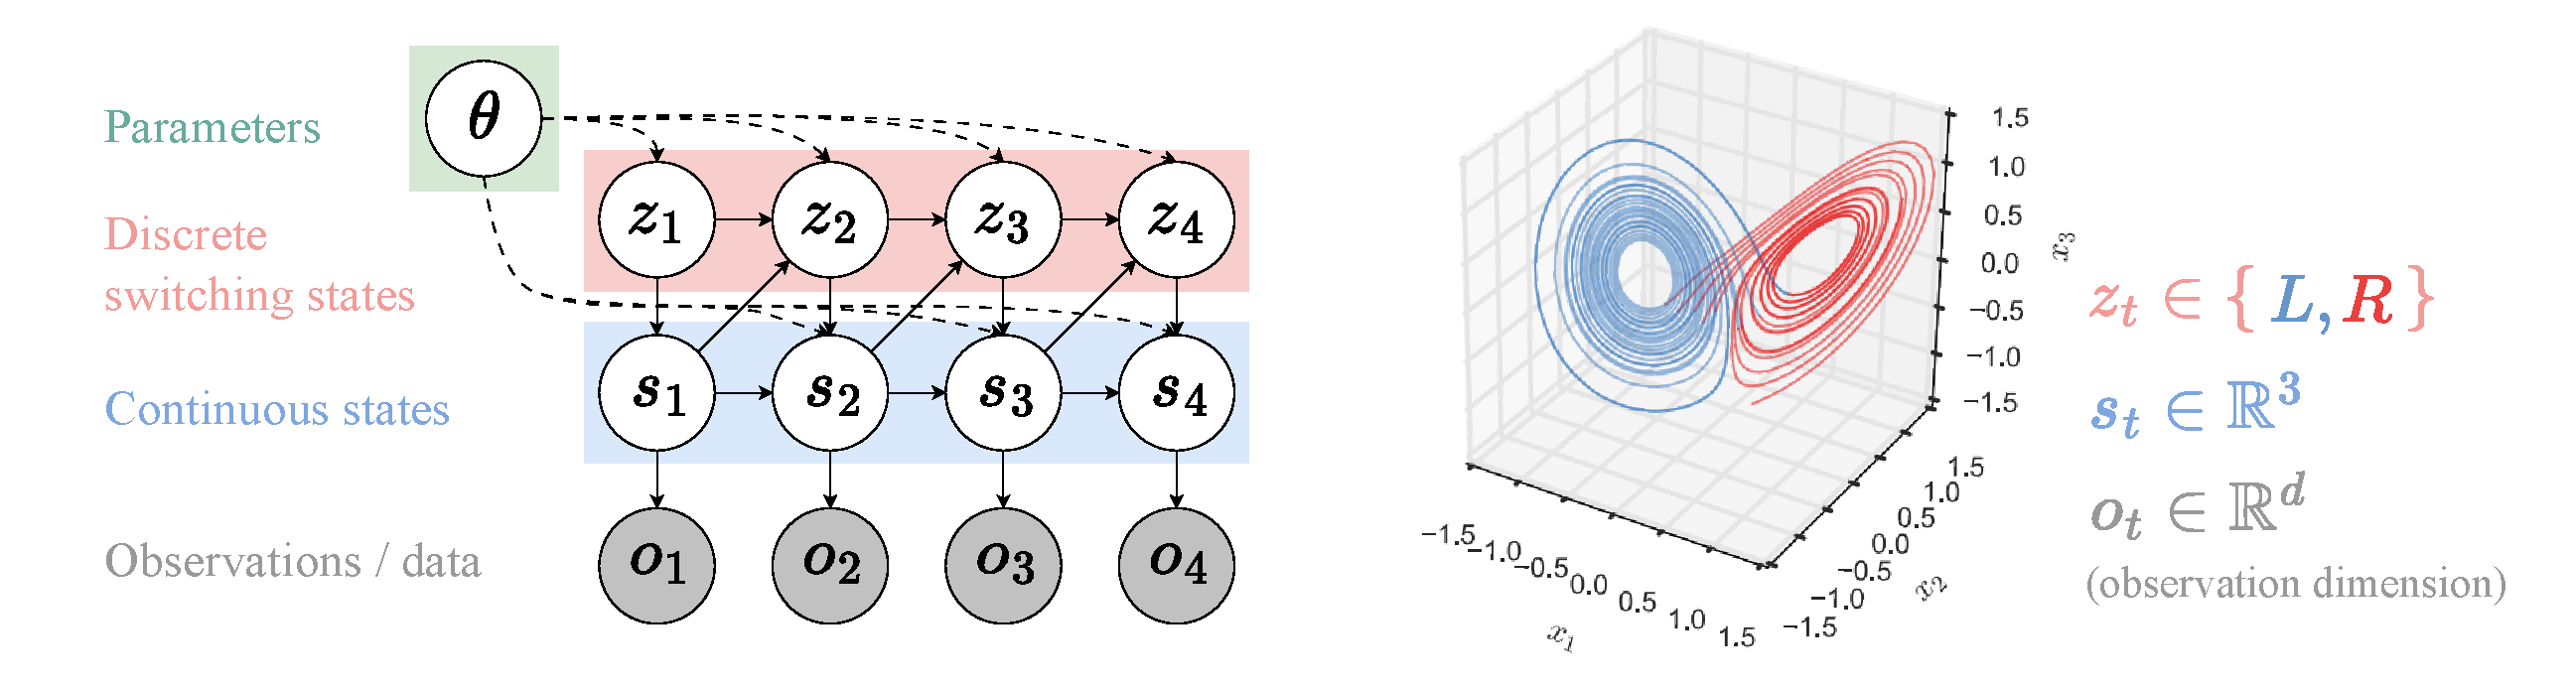
\includegraphics[width=\linewidth]{changepoints/figs/sds.pdf}   \vspace{-1em}
	\caption{(Left) Generative model of the SDS dynamics as in \Eqref{eq:sds}. Shaded circles represent observed  variables; hollow circles are latent variables. (Right) Example to illustrate notation. We show a Lorenz attractor, a canonical nonlinear dynamical system, approximated by a linear SDS \cite{linderman2023slds}.}
	\label{fig:sds_figure}
         \vspace{-1.5em}
\end{figure}

Switching dynamics systems (SDS), or mixed dynamics systems, provide a powerful framework for modeling time series with change points, where the underlying dynamics shift between distinct regimes. SDS assumes the system consists of a total of $K$ different base dynamics. It explicitly incorporates discrete switching \textit{states} to represent the abrupt shifts among base dynamics. We denote the discrete switching states at timestep $t$ as $z_t \in \mathcal{Z}$, $ \mathcal{Z} = \{1, \dots, K\} \subset \mathbb{Z}^+$, to index one of $K$ base dynamical systems, and represent the observed sequence as ${o_1, \ldots, o_T }$ or $o_{1:T}$ for conciseness. %Since continuous states $s_t$ are rarely discussed, we use \textit{state} to refer to discrete states $z_t$ if not otherwise indicated.

There have been many different variations and implementations of SDS.  Classic SDS have \textit{memory-less} state transitions, i.e. $p(z_t|z_{t-1})$ is parameterized by a stochastic transition matrix $\mathbf{A}\in \R ^{K \times K}$. 
This results in an “open loop” system and the state  duration follows a geometric distribution. Recent works have sought to fix this issue, for example by closing the loop using recurrent dependencies on $s_t$ \citep{linderman2016recurrent}, or modeling explicit durations \citep{ansari2021deep}. Our generative model is illustrated in figure \ref{fig:sds_figure}): for generality, we factor out any non-Markovian covariates to model parameters $\theta$. The joint distribution can be factorized as
\vspace{-1em}
\begin{equation} \label{eq:sds}    
\begin{split} 
& P(o_{1:T}, s_{1:T}, z_{1:T} ) =  \prod^T_{t=1} P(o_t | s_t) P(s_t| s_{t-1}, z_t, \theta) P(z_t| s_{t-1}, z_{t-1},\theta)
\end{split}
\end{equation}

\vspace{-1.5em}
where $p(s_1|z_1)p(z_1)$ is the initial state prior. The $K$ dynamical systems have continuous state transition $p(z_t|z_{t-1}, s_{t-1}, \theta)$, and the emission  $p(o_t| s_t)$ can be linear or nonlinear (e.g. parameterized by a neural network). Moreover, the SDS framework naturally supports forecasting both the next observation \(o_{t+1}\) via
$P(o_{t+1}\mid s_{t+1})$
and the next switching state \(z_{t+1}\) via
$P(z_{t+1}\mid s_t, z_t, \theta).$


\section{Conformal Prediction for Time series with Change points (CPTC)}
We introduce CPTC, a novel conformal prediction algorithm that utilizes the state prediction from SDS to improve uncertainty quantification for time series forecasting.
\vspace{-0.5em}
\paragraph{Problem Setting}
% Consider a sequential prediction problem over data generated by the SDS dynamics as illustrated in section \ref{background:sds}, whose observations $o_t \in \R^d$ for all $t$. 
We are given a sequence of observations $o_t \in \R^d$ for all $t$ potentially with  change points.
To be consistent with the standard notation in conformal prediction literature, let 
$\mathcal{X} \subseteq \R^{m}$ denote the input feature domain and $\mathcal{Y} \subseteq \R^d$ the target observation space. $ \mathcal{Z} = \{1, \dots, K\} \subset \mathbb{Z}^+$ indexes one of $K$ underlying states. The input features can include past observations and other environmental covariates.  In our implementations, $m = k \cdot d$ with $k$ being the look back window.

We consider the online conformal prediction setting where we have a sequence of data points from $\mathcal{X} \times \mathcal{Y}$: $(x_1, y_1), $ $(x_2, y_2), \ldots, (x_T , y_T )$. We have a trained state predictor for $\hat{p}(z_t|x_{0:t})$ , a state-conditioned forecaster $\hat{f}:\gX \times \gZ \to \gY$ (a probabilistic SDS model can serve both purposes), and are given a desired confidence level $1-\alpha$. At each time step $t$, we have seen $(x_1, y_1),(x_2, y_2), \ldots,(x_{t-1} , y_{t-1} )$ and the next input feature vector $x_t$. We want to produce an adaptive, time-dependent prediction interval based on input $\Gamma_t(x_t) \subseteq \mathcal{Y}$ for the unseen true target $y_t$, which we will learn at the next time step. Let $z_t \in \gZ$ be the true (latent switching) state at time $t$. %We assume that we have access to a model for probabilistic forecast $\hat{p}(z_t=z|x_{0:t})$ of the latent state at each timestep. %nonconformity score function $A(x, y): \mathcal{X} \times \mathcal{Y} \rightarrow \R_{\geq 0}$   kkfldldldfk;sdf%, denoted as $\hat{z_t}$, and a dynamics forecaster model for each mode $ \hat{f}_z$. 
Our goal is to produce prediction intervals with correct empirical coverage, i.e.    
\vspace{-0.2em}
\begin{equation}
    P (y_t \in \Gamma_t(x_t)) \geq 1-\alpha \; \text{ for any } t\geq 0
    \label{eq:goal}
\end{equation}
\vspace{-2em}
\subsection{Algorithm}
Existing online conformal prediction algorithms often rely on assumptions about how distribution would shift in time series. This is infeasible for data with change points due to  unknown shift mechanism. The main contribution our algorithm makes towards addressing this issue is \textit{anticipating} this type of abrupt shifts. 
Our CPTC algorithm is outlined in pseudo-code in algorithm \ref{alg:cptc}. In this section, we discuss the general procedure and key components of the algorithm. 


%\begin{wrapfigure}{r}{0.5\textwidth}
% \begin{wrapfigure}{L}{0.6\textwidth}
% \begin{minipage}{0.6\textwidth}

\begin{algorithm}[H]%[tb]
   \caption{Conformal Prediction for Time series with Change points (CPTC)}
   \label{alg:cptc}
   \SetAlgoLined
   \KwIn{nonconformity score function $A$, probabilistic state model $\hat{p}(z_t|x_{0:t})$ with prior $\hat{p}(z_0)$, forecaster model $\hat{f}: \mathcal{X}\times \mathcal{Z} \rightarrow \mathcal{Y} $, confidence level $1- \alpha$, learning rate $\gamma$}
   \KwOut{Prediction intervals $\Gamma(x_t)$ for $t \geq 1$}
   
   \For{$z \in \mathcal{Z}$}{
       Initialize $\gS_z \leftarrow \{\}$,  $\alpha_{z,0} \leftarrow \alpha$ 
   }
   \If{exists warm start data $\{(x_t, y_t)\}_{t=-w}^{0}$}{
       \For{$t \in [-w,0]$}{
        $\gS_{z_t} \leftarrow \gS_{z_t} \cup \{A(x_t, y_t)\}$, where $z_t \sim \hat{p}(z_t = z |x_{0:t})$; \tcp{warm start scores} 
       }
   }
   \For{$t \in [1,T]$}{
       \For{$z \in \mathcal{Z}$}{
           $\Gamma_{z,t}(x_t) \leftarrow \{ y : A(x_t, y) \leq Q^{1-\alpha_{z,t}}(\gS_z \cup \{\infty\})\}   $; \tcp{state-specific CP} %Conformal prediction interval with forecaster $\hat{f}(x_t,z)$, confidence level $1-\alpha_{z,t}$, calibrated on $\gS_z$\;
       }
       $\Gamma_t(x_t) \leftarrow$ Aggregate the $\Gamma_{z,t}(x_t)$s by \Eqref{eq:aggregation-average} or \Eqref{eq:aggregation-union}\;
       \KwOut{$\Gamma_t(x_t)$}
       Sample state $\hat{z}_t \sim \hat{p}(z_t|x_{0:t})$; \tcp{state-specific coverage target tracking}
       Update $\alpha_{\hat{z}_t, t+1} \leftarrow \alpha_{\hat{z}_t, t} + \gamma \cdot (\alpha - err_t)$, where $err_t = \mathbbm{1}\{y_t \notin \Gamma_t(x_t)\}$\;
       Update scores $\gS_{\hat{z}_t} \leftarrow \gS_{\hat{z}_t} \cup \{A(x_t, y_t)\}$\;
   }     
   \end{algorithm}
  %   \end{minipage}
  % \end{wrapfigure}



\vspace{-0.5em}
\paragraph{Switching Behavior and SDS Integration.}
We explicitly model the abrupt shift in dynamics with the switching dynamical systems (SDS) to anticipate the change. In our formulation, the latent state \(z_t\) indicates which dynamical regime (out of \(K\) possible regimes) is currently active at time \(t\). Given the SDS formulation (e.g. \Eqref{eq:sds}), we can factor the state transition probability from the conformal prediction process and do calibration for each of the $K$ dynamics separately. The goal in \Eqref{eq:goal} can therefore be written as:
%
\begin{equation}
    \sum_{z\in\gZ} P(y_t \in \Gamma_t(x_t)| z_t=z) \; P(z_t = z|x_{0:t}) \geq 1-\alpha 
\label{eq:factored_goal}
\end{equation}
\vspace{-1.2em}
\paragraph{State Prediction.} The SDS model provides us with the state predictor \(\hat{p}(z_t \mid x_t)\). In practice, SDS models \cite{ansari2021deep, linderman2016recurrent} have existing $z_t$ forecasts that we can extract. For other model architectures, one can modify them to output an extra covariate prediction for the state, or add an auxiliary model to classify or cluster the input space into different regimes. In practice, $z_t$ doesn’t necessarily have to come from a model, and can be any discrete contextual variable such as weekday/weekend/holiday or day/night.

\vspace{-0.5em}
\paragraph{Initialization and Warm Start,} For each switching state $z \in Z$, we initialize (1) a mode-specific set of nonconformity scores $\gS_z$ and (2) the mode-specific confidence level $\alpha_{z,0} = \alpha$. If there are $w$ steps of warm-start data $\{(x_t,y_t)\}_{t=-w}^0$, we initialize the sore sets $\gS_z$ by sampling $z_t \sim \hat{p}(z_t = z |x_{0:t})$ for $t= -w, \ldots, 0$, and inserting $A(x_t,y_t)$ into $\gS_{z_t}$. Depending on the size of the warm-start window and desired properties, practitioners can adjust the warm-starting approach. For example, using the entire warm-start window $\gS_{z} = \{A(x_t,y_t)\}_{t=-w}^0$  for all $z \in \gZ$  will result in better stability but less adaptability to modes. The approach does not change the algorithm's coverage guarantees. 

\vspace{-0.5em}
\paragraph{State-Specific Prediction Intervals.}  At every time step $t\in [1, T]$, CPTC creates state-specific conformal prediction intervals
for all states with nonzero probability. This allows us to generate predictions tailored to the current anticipated dynamics. Specifically, for every state $z\in \gZ$ where $\hat{p}(z|x_{0:t}) > 0$, we first obtain the point prediction through forecaster model $\hat{f}(x_t, z)$, and then the state-specific prediction interval $\Gamma_{z,t}(x_t)$ by calibrating on nonconformity scores set $\gS_z$ to the adaptive confidence level of $1-\alpha_{z,t}$.


\vspace{-0.5em}
\paragraph{Online Conformal Prediction.}
The exchangeability assumption does not apply to the online setting of our work. If we naively calibrate with online data, when the data distribution changes, the coverage probability may deviate from the target level $1-\alpha$. Therefore, we follow online CP methods such as ACI \citep{gibbs2021adaptive} to address this problem by continuously updating $\alpha_{z,t}$ to track a surrogate miscoverage rate $\alpha_{z,t}^*$ as defined in \eqref{eq:alpha_star} (for each state $z$ in our setting), an internal estimate of the target coverage.
%
\begin{equation}
    \alpha^*_{z,t} = \sup\{\beta \in [0, 1] : M_{z,t}(\beta) \leq \alpha\}, \; M_{z,t}(\alpha) = p(A(x_t, y_t) > Q^{1 - \alpha}(\gS_z))  
    \label{eq:alpha_star}
\end{equation}
%
In \eqref{eq:alpha_star} $M_{z,t}$ measures the probability that the true label $y_t$ falls outside the prediction set $\Gamma_{z,t}$ when the predicted state is $z$. %$M_t(\alpha)$ may not be equal to $\alpha$ due to distribution shifts. 
We track $\alpha^*_{z,t}$ over time by updating the estimate $\alpha_{z,t}$ with online optimization. In our implementation, we use the simple update from ACI (\Eqref{eq:aci_update}), though more sophisticated approaches such as \citep{angelopoulos2024pid} may be used in its place without affecting the overall algorithm.
\begin{equation}
\alpha_{\hat{z}_t, t+1} \leftarrow \alpha_{\hat{z}_t, t} + \gamma \cdot (\alpha - err_t), \; \text{where } err_t = \mathbbm{1} \{y_t \notin \Gamma_t(x_t) \}
\label{eq:aci_update}
\end{equation}
Here $\gamma > 0$ is the step size hyperparameter, and $\hat{z}_t \in \gZ, \; \hat{z}_t \sim \hat{p}(z_t = z |x_{0:t})$ is the state at time $t$ sampled to be updated. The update rule increases $\alpha_{\hat{z}_t, t}$ if coverage is too conservative and decreases it otherwise, ensuring that for each $z \in \gZ$, $\alpha_{z,t}$ converges to a value that maintains long-term coverage. 


\vspace{-0.5em}
\paragraph{Aggregation.} We aggregate the prediction intervals for each state $\Gamma_{z,t}(x_t)$ into one final set $\Gamma_{t}(x_t)$ using the weighted level set, as illustrated in \Eqref{eq:aggregation-average}. %The weighted approach results in sharp prediction intervals, but may risk slightly lower coverage if the classifier for $z$ is imperfect.
%
\begin{equation}
\Gamma_t(x_t) :=  \bigl\{ y:  \sum_{z \in \mathcal{Z}}
\hat{p}\bigl(z_t = z \mid x_t\bigr)
\mathbbm{1}\{\,y \in \Gamma_{z,t}(x_t)\} 
\geq 1 - \alpha \bigr\}
\label{eq:aggregation-average}
\end{equation}

\vspace{-0.8em}
Solution to the constraint in \Eqref{eq:aggregation-average}  is the minimal set that achieves the marginal coverage. It can be obtained through discretizing $\mathcal{Y}$ into a fine grid and calculating probability mass at each point, which becomes computationally expensive as the grid resolution or dimensionality increases. For faster computation and in implementation, we approximate the weighted level‐set in \Eqref{eq:aggregation-average} by taking the union of intervals of the most probable states as in \Eqref{eq:aggregation-union}. The two aggregation strategies achieve similar results on all our datasets (Appendix \ref{app:more_experiments}).
%
%Alternatively, we can opt for a more conservative aggregation by taking the union of intervals of the probable states as in  \sofi{explain why they are not far, explain approx eq}
%Alternatively, if finding the set in Eq. \ref{eq:aggregation-average} is challenging or there are high uncertainty for the state classifier, we can opt for a more conservative relaxation. Aggregation by taking the union (Eq. \ref{eq:aggregation-union}) results in larger sets and guaranteed validity over time. 
 \begin{equation}
    \Gamma_t(x_t) \approx \cup_{z\in \mathcal{Z}'_t} \Gamma_{z,t}(x_t), \; 
    \text{where } \mathcal{Z}'_t
=\;\underset{S\subseteq\mathcal Z}{\arg\min}\;\bigl\lvert S\bigr\rvert
\;\text{s.t.}\;\sum_{z\in S}p(z_t=z\mid x_t)\;\ge\;1-\alpha.
    \label{eq:aggregation-union}
\end{equation}
%
\vspace{-1.5em}
\paragraph{Modularity and the role of the state model.} Our algorithm can be viewed as running multiple instances of online conformal inference (lines 14-16 of algorithm \ref{alg:cptc}), one for each underlying state, and adaptively aggregating the confidence intervals when the underlying mode is switching. This differs from the setting where the temporal correlation between residuals needs to be learned online \citep{gibbs2024conformal, bastani2022practical, xu2023sequential, auer2023hopcpt}; the state model allows us to leverage training data for such information. Our algorithm is modular - the state model, forecaster model, and the online adaptive conformal prediction algorithms all operate independently of each other. For example, the state-specific online coverage tracking (line 15 of algorithm \ref{alg:cptc}) can be replaced with other online conformal prediction variants for data-specific applications. Our theoretical guarantees are agnostic to the forecaster models used. %If the forecasters and the state model are re-trained, our algorithm will adapt to the new model while still achieving asymptotic coverage. Section \ref{sec:theory} will elaborate on this claim. 



\subsection{Theoretical analysis}
\label{sec:theory}

In this section, we discuss theoretical guarantees of the CPTC algorithm. In particular, we establish finite-sample validity under exchangeability, asymptotic coverage in dynamic (potentially nonstationary) settings, robustness to imperfect state classification, and faster adaptation to distribution shifts that align with model-predicted state changes. See Appendix \ref{app:proofs} for proofs and theoretical details.

\vspace{-0.5em}
\paragraph{Finite-sample validity under exchangeability.}
We start by showing that when data is exchangeable (e.g. independent and identically distributed), CPTC achieves finite sample validity. The proof is standard based on showing the marginal coverage of split conformal prediction. 

\begin{proposition}[Finite-sample validity under exchangeability] If the data $(x_t, y_t)$, $t \geq 1$ are exchangeable, prediction intervals obtained via Algorithm \ref{alg:cptc} satisfy
\( P(y_t \in \Gamma_t(x_t)) \geq 1-\alpha\).
\label{prop:exchangable}
\end{proposition}

\vspace{-0.5em}
\paragraph{Asymptotic validity without assumptions.}
%\vspace{-0.3em}
Theorem \ref{thm:asymptotic_validity} ensures that CPTC provides reliable uncertainty quantification in the long run \textit{without assumptions on time-series stationarity or accurate state predictions}. (We do assume that the distribution of states and state predictions exhibit stable long-term behavior in Assumption \ref{assump:stationary_distribution}.) We achieve our desiderata of \Eqref{eq:goal} on average as $T$ grows asymptotically, consistent with the results of other online conformal prediction works. 

%
\begin{theorem}[Asymptotic validity of CPTC] \label{thm:asymptotic_validity}
For any sample size \( T \geq 1 \), the CPTC algorithm (with weighted average aggregation) achieves:
\begin{equation*}
    \left| \frac{1}{T} \sum_{t=1}^T \mathbb{E}[err_t] - \alpha \right| \leq  \frac{1}{T} \sum_{z=1}^K  \frac{ 1 - (1-c\gamma)^{|\mathcal{T}_z|}  }{\gamma} |\alpha - \alpha^{*}_z|
    \label{eq:thm1}
\end{equation*}
Where:
\vspace{-4mm}
\begin{itemize}  \setlength{\itemsep}{0pt plus 1pt}
    \item \(\text{err}_t = \mathbbm{1}[Y_t \notin \Gamma_{t}(x_t)]\), the miscoverage rate. 
    \item \( \mathcal{T}_z = \{ t \in \{1, \dots, T\} : \hat{z}_t = z \} \), the set of time steps the predicted state is \( z \).
    \item $\alpha^*_z$ is the optimal miscoverage target for timesteps $\mathcal{T}_z$.
    \item  $c$ is a miscoverage constant in Lemma \ref{lemma:aci_within_states} \cite{gibbs2021adaptive}. 
\end{itemize}
\vspace{-0.5em}
Note the RHS of \Eqref{eq:thm1} decays at a rate of $\mathcal{O}(T)$ and satisfies
 \(
 \lim_{T \to \infty} \left| \frac{1}{T} \sum_{t=1}^T \mathbb{E}[err_t] - \alpha \right|= 0
 \).
\end{theorem}

%Importantly, the algorithm adapts dynamically to stabilize its coverage as the time horizon increases.

\vspace{-0.5em}
\paragraph{Robustness to imperfect state prediction.}
In real-world applications, the state predictor  $\hat{p}(z_t|x_{0:t})$ that plays a large role in our algorithm is often imperfect. The CPTC algorithm accommodates these scenarios by tracking $\alpha^*_{z}$ for each \textit{predicted} mode $z$ with adaptive online updates. Theorem \ref{thm:imperfect_state_predictions} quantifies the effect of imperfect state prediction by showing that the miscoverage rate is bounded by the product of the misclassification rate and state-specific deviations. 
%
\vspace{0.1em}
\begin{theorem}[Finite-Sample Miscoverage Bound with Imperfect State Predictions]\label{thm:imperfect_state_predictions}
For any sample size \( T \geq 1 \), the CPTC algorithm ensures that:
\vspace{-0.2em}
\[
\left| \frac{1}{T} \sum_{t=1}^{T} \mathbb{E}[err_t]  - \alpha \right| \leq \epsilon \cdot \max_z \delta_{z,T}
\]

\vspace{-1em}
Where \( \epsilon = P(\hat{z}_t \neq z_t) \) is the error rate of the state predictions and \( \delta_{z,T} \) is the miscoverage deviation from \( \alpha \) for any predicted state $z$ defined in Lemma \ref{lemma:aci_within_states}. For all $z$, \( \delta_{z,T} \to 0 \) as \( |T| \to \infty \).
%\vspace{-4mm}
% \begin{itemize}\setlength{\itemsep}{0pt plus 1pt}
    %\item \(\text{err}_t := \mathbb{I}\big(Y_t \notin \Gamma_{CPTC}(x_t)\big)\), the miscoverage rate. 
    %\item \( \mathcal{T}_z = \{ t \in \{1, \dots, T\} : \hat{z}_t = z \} \), the set of times when the predicted state is \( z \).
    %\item \( z_t \) denotes the true latent state at time \( t \), and \( \hat{z}_t \) the predicted state. 
%     \item \( \epsilon = P(\hat{z}_t \neq z_t) \) is the error rate of the state predictions.
%     \item \( \delta_{z,T} \) is the miscoverage deviation from \( \alpha \) for any predicted state $z$ defined in Lemma \ref{lemma:aci_within_states}. For all $z$, \( \delta_{z,T} \to 0 \) as \( |T| \to \infty \).
% \end{itemize}
\end{theorem}

Theorem \ref{thm:imperfect_state_predictions} demonstrates that CPTC can maintain asymptotic valid coverage even when state predictions are imperfect, with the bound tightening as state predictions improve or the number of observations per state increases. In practice, improving the accuracy of the state prediction model directly enhances the coverage performance of CPTC. However, even with imperfect state predictions, the algorithm's adaptive calibration mechanism ensures that the overall coverage remains close to the desired level \(1 - \alpha\) as experiments show in Section \ref{sec:accuracy}.

%\subsubsection{Validity for union aggregation}

%As noted in the methodology section, if we use set union as the aggregation approach, CPTC will produce more conservative prediction intervals aiming for overcoverage. 

%By leveraging the union of prediction sets across all possible states, CPTC ensures that the algorithm maintains valid coverage, even in the presence of uncertainty during state transitions.

% \begin{proposition}[Conservative Coverage Guarantee of CPTC on Transition States]
% Note that \(\Gamma_t(x_t) = \bigcup_{z \in Z} \Gamma_{z,t}(x_t)\) is the prediction set produced by the CPTC algorithm at time \(t\).
% then the overall prediction set \(\Gamma_t(x_t)\) provides conservative coverage, meaning:
% \begin{equation}
% P(y_t \in \Gamma_t(x_t)) \geq 1 - \alpha
% \end{equation}
% for all \(t\).
% \end{proposition}

% This is because (1)  \(P(y_t \in \Gamma_{z,t}(x_t) | z_t = z) \geq 1 - \alpha_{z,t}\) for all \(t\) (i.e., the conditional coverage given state \(z\) is at least \(1 - \alpha_{z,t}\)), and (2)  \(\lim_{T_z \to \infty} (1/T_z) \sum_{t=1}^{T_z} \alpha_{z,t} \leq \alpha\) where \(T_z\) is the number of time steps where state \(z\) is predicted. 
\vspace{-0.3em}
\paragraph{Why CPTC? Faster convergence under distribution shifts.}

The strength of the CPTC algorithm is its fast adaptation in dynamic environments with distributional changes. When a distribution shift aligns with a predicted state transition, the structure of CPTC allows the confidence level $\alpha_{z,t}$ to converge to the new target error rate faster compared to purely online methods.

Consider a data stream with a distribution shift occurring at time $t_{{\text{shift}}}$. Let $\alpha^*_{j}$ denote the optimal target error rate for mode $j$ after the shift, and assume that the predicted state $\hat{z}_t$ correctly reflects the shift: $t_{\text{shift}}$ and $\alpha^*_{z} = \alpha^*_{j}$ for $t > t_{{\text{shift}}}$. For conciseness of notation in Theorem \ref{thm:adaptation}, let $\delta_{j,T}$ and $\delta_{ACI,T}$ denote the miscoverage rate \textit{starting from } $t_{\text{shift}}$ for CPTC and ACI respectively.

\vspace{0.1em}
\begin{theorem}[Miscoverage Ratio under State-Coincident Distribution Shift]
Under a state shift from $i$ to $j$ at time step $t_{\text{shift}}$, coinciding with predicted transition, the CPTC algorithm achieves faster convergence to the new target $\alpha^*_{j}$ compared to non-state-aware algorithm ACI at a ratio of:
\[
\frac{\delta_{j,T}}{\delta_{\text{ACI},T}} \leq \frac{|\alpha_{j, t_{\text{shift}}-1}  - \alpha^{*}_{j}|}{|\alpha_{ t_{\text{shift}}-1} - \alpha^{*}_{j}|}
\]
\label{thm:adaptation}
\end{theorem}
\vspace{-1em}
%
The numerator $|\alpha_{j, t_{\text{shift}}-1}  - \alpha^{*}_{j}| \rightarrow 0$ as $T \rightarrow \infty$, when in-state adaptation has converged; but the denominator $|\alpha_{ t_{\text{shift}}-1} - \alpha^{*}_{j}|$ remains greater than zero regardless of the length of the time series. This result highlights the advantage of segmenting nonconformity scores by state: the state-specific $\alpha_{z,t}$ aligns the target miscoverage updates with distribution shifts, allowing CPTC to quickly adjust its prediction intervals. Such accelerated adaptation allows for shorter miscoverage periods and is critical in real-world applications where rapid responses to changing conditions are necessary.
%Theorem \ref{thm:adaptation} shows that CPTC's bound is smaller by a factor that depends on the ratio of the distances of the original $\alpha$ and $\alpha_{i}^*$ from the new optimum $\alpha_{j}^*$, as well as the ratio of the segment lengths.



\section{Experiments}


% \begin{table*}[bh]
% \vspace{-0.8em}
% \caption{Performance on synthetic and real-world datasets with target confidence $1-\alpha = 0.9$ (for horizon $T=200$ for synthetic datasets, $300$ for electricity and traffic, and $60$ for bee, mean $\pm$ standard deviation of the test samples).  Methods that are \textit{invalid} (coverage below $90\%$) are grayed out. Our method achieves a high level of calibration (coverage is close to $90\%$) consistently. }
% \label{tab:baselines}
% \centering
% \resizebox{\textwidth}{!}{%
% \begin{tabular}{ l | c | c  c c c c c } 
% \toprule
% & & RED-SDS & CP & ACI & SPCI  & HopCPT & Ours \\ 
% \midrule\midrule
% \multirow{2}{*}{\begin{tabular}{l}Bouncing  \\ Ball obs.\end{tabular}} & Cov & \color{gray}{59.14 \plusminus 23.75}& \color{gray}{39.27 \plusminus 6.77}& \color{gray}{76.97 \plusminus 1.27}& \color{gray}{37.90 \plusminus 9.78}& \color{gray}{59.45 \plusminus 12.51} &91.03 \plusminus 1.37\\ 
%  & Width & \color{gray}{2.12 \plusminus 0.05}& \color{gray}{1.71 \plusminus 0.93}& \color{gray}{3.67 \plusminus 0.91}& \color{gray}{1.45 \plusminus 0.85}& \color{gray}{1.98 \plusminus 0.90} & 2.13 \plusminus 2.15\\ 
% \midrule
% \multirow{2}{*}{\begin{tabular}{l}Bouncing  \\ Ball dyn.\end{tabular}} & Cov & \color{gray}{43.46 \plusminus 27.18}& \color{gray}{40.41 \plusminus 6.89}& \color{gray}{76.63 \plusminus 0.95}& \color{gray}{53.62 \plusminus 7.75}& \color{gray}{61.12 \plusminus 4.80} &90.44 \plusminus 1.51\\ 
%  & Width & \color{gray}{1.80 \plusminus 0.03}& \color{gray}{0.89 \plusminus 0.45}& \color{gray}{2.97 \plusminus 1.07}& \color{gray}{2.02 \plusminus 0.23}& \color{gray}{2.95 \plusminus 1.12} & 4.92 \plusminus 2.79\\ 
% \midrule
% \multirow{2}{*}{\begin{tabular}{l}3-Mode \\ System\end{tabular}} & Cov & 92.98 \plusminus 3.01& \color{gray}{63.97 \plusminus 5.03}& \color{gray}{86.25 \plusminus 0.84}& \color{gray}{81.72 \plusminus 2.88}& 89.85 \plusminus 2.90 & 93.35 \plusminus 3.51\\ 
%  & Width & 2.08 \plusminus 0.16& \color{gray}{1.46 \plusminus 0.51}& \color{gray}{2.61 \plusminus 0.53}& \color{gray}{3.94 \plusminus 0.85}& 9.07 \plusminus 1.23 &  13.68 \plusminus 2.49\\ 
% \midrule
% \midrule
% \multirow{2}{*}{\begin{tabular}{l}Traffic\end{tabular}} & Cov & \color{gray}{86.55 \plusminus 11.20}& \color{gray}{69.64 \plusminus 2.62}& \color{gray}{88.19 \plusminus 0.33}& 88.24 \plusminus 2.13& 88.91 \plusminus 3.55 & 94.76 \plusminus 4.93\\ 
%  & Width & \color{gray}{2.81 \plusminus 1.54}& \color{gray}{0.32 \plusminus 0.22}& \color{gray}{56.92 \plusminus 25.26}& 4.62 \plusminus 2.28 & 7.50 \plusminus 10.09 & 8.34 \plusminus 14.44\\ 
% \midrule
% \multirow{2}{*}{\begin{tabular}{l}Electricity\end{tabular}} & Cov & \color{gray}{75.46 \plusminus 14.23}& \color{gray}{68.88 \plusminus 3.12}& \color{gray}{87.94 \plusminus 0.34}& \color{gray}{86.62 \plusminus 2.97} & \color{gray}{86.50 \plusminus 2.66} & 92.62 \plusminus 6.14\\ 
%  & Width & \color{gray}{87.47 \plusminus 119.95}& \color{gray}{58.62 \plusminus 456.89}& \color{gray}{28.28 \plusminus 169.33}& \color{gray}{371.69 \plusminus 305.86}& \color{gray}{155.71 \plusminus 130.43} & 166.88 \plusminus 129.07 \\ 
% \midrule
% \multirow{2}{*}{\begin{tabular}{l}Dancing \\ Bees\end{tabular}} & Cov & 90.79 \plusminus 5.03& \color{gray}{65.58 \plusminus 7.05}& \color{gray}{75.16 \plusminus 3.33}& \color{gray}{79.2 \plusminus 0.3} & \color{gray}{72.11 \plusminus 1.84} & 93.43 \plusminus 11.42 \\
%  & Width & 0.27 \plusminus 0.05& \color{gray}{0.12 \plusminus 0.01}& \color{gray}{1.77 \plusminus 1.38}& \color{gray}{1.77 \plusminus 1.38} & \color{gray}{1.06 \plusminus 0.51} & 1.15 \plusminus 0.56 \\
% \bottomrule
% \end{tabular}
% }
% \vspace{-0.5em}
% \end{table*}

\begin{table*}[bh]
\vspace{-0.8em}
\caption{Performance on synthetic and real-world datasets with target confidence $1-\alpha = 0.9$ (for horizon $T=200$ for synthetic datasets, $300$ for electricity and traffic, and $60$ for bee, mean $\pm$ standard deviation of the test samples).  Methods that are \textit{invalid} (coverage below $90\%$) are grayed out. Our method achieves a high level of calibration (coverage is close to $90\%$) consistently. }
\label{tab:baselines}
\centering
\resizebox{\textwidth}{!}{%
\begin{tabular}{ l | c | c  c c c c c } 
\toprule
& & RED-SDS & CP & ACI & SPCI  & HopCPT & Ours \\ 
\midrule\midrule
\multirow{2}{*}{\begin{tabular}{l}Bouncing  \\ Ball obs.\end{tabular}} & Cov & \color{gray}{16.90 \plusminus 12.96} & \color{gray}{87.67 \plusminus 6.54} & \color{gray}{89.82 \plusminus 2.95} & \color{gray}{87.13 \plusminus 4.79} & \color{gray}{59.45 \plusminus 12.51} & 90.15 \plusminus 1.19\\ 
 & Width & \color{gray}{1.60 \plusminus 0.07} & \color{gray}{10.54 \plusminus 3.19} & \color{gray}{3.85 \plusminus 2.60} & \color{gray}{2.82 \plusminus 0.41} & \color{gray}{1.98 \plusminus 0.90} & 3.71 \plusminus 0.98\\ 
\midrule
\multirow{2}{*}{\begin{tabular}{l}Bouncing  \\ Ball dyn.\end{tabular}} & Cov & \color{gray}{13.20 \plusminus 11.50} & \color{gray}{86.45 \plusminus 12.28} & \color{gray}{89.38 \plusminus 2.56} & \color{gray}{53.62 \plusminus 7.75} & \color{gray}{61.12 \plusminus 4.80} & 90.47 \plusminus 2.30\\ 
 & Width & \color{gray}{1.37 \plusminus 0.05} & \color{gray}{11.49 \plusminus 4.39} & \color{gray}{2.27 \plusminus 1.65} & \color{gray}{2.02 \plusminus 0.23} & \color{gray}{2.95 \plusminus 1.12} & 1.76 \plusminus 0.71\\ 
\midrule
\multirow{2}{*}{\begin{tabular}{l}3-Mode \\ System\end{tabular}} & Cov & 93.02 \plusminus 3.04 & \color{gray}{63.98 \plusminus 5.04} & \color{gray}{89.90 \plusminus 2.25} & \color{gray}{84.90 \plusminus 5.41} & 89.85 \plusminus 2.90 & 94.96 \plusminus 1.96\\ 
 & Width & 2.08 \plusminus 0.16 & \color{gray}{1.46 \plusminus 0.50} & \color{gray}{6.40 \plusminus 1.92} & \color{gray}{3.70 \plusminus 0.89} & 9.07 \plusminus 1.23 & 2.45 \plusminus 0.72\\ 
\midrule
\midrule
\multirow{2}{*}{\begin{tabular}{l}Traffic\end{tabular}} & Cov & \color{gray}{23.15 \plusminus 10.95} & \color{gray}{87.06 \plusminus 3.71} & 90.01 \plusminus 0.87 & \color{gray}{84.38 \plusminus 2.47} & 88.91 \plusminus 3.55 & 92.38 \plusminus 1.24\\ 
 & Width & \color{gray}{0.05 \plusminus 0.02} & \color{gray}{21.91 \plusminus 10.42} & 27.81 \plusminus 54.08 & \color{gray}{5.32 \plusminus 1.95} & 7.50 \plusminus 10.09 & 7.92 \plusminus 2.98\\ 
\midrule
\multirow{2}{*}{\begin{tabular}{l}Electricity\end{tabular}} & Cov & \color{gray}{62.85 \plusminus 13.67} & \color{gray}{85.69 \plusminus 6.17} & \color{gray}{89.79 \plusminus 0.83} & \color{gray}{84.10 \plusminus 2.77} & \color{gray}{86.50 \plusminus 2.66} & 91.22 \plusminus 1.29\\ 
 & Width & \color{gray}{162.67 \plusminus 811.73} & \color{gray}{366.05 \plusminus 2280.45} & \color{gray}{45.74 \plusminus 279.21} & \color{gray}{228.14 \plusminus 1207.58} & \color{gray}{155.71 \plusminus 130.43} & 139.75 \plusminus 620.44\\ 
\midrule
\multirow{2}{*}{\begin{tabular}{l}Dancing \\ Bees\end{tabular}} & Cov & \color{gray}{84.92 \plusminus 6.84} & \color{gray}{79.86 \plusminus 20.73} & \color{gray}{86.25 \plusminus 8.10} & \color{gray}{79.20 \plusminus 0.30} & \color{gray}{72.11 \plusminus 1.84} & 92.64 \plusminus 3.19\\
 & Width & \color{gray}{0.25 \plusminus 0.02} & \color{gray}{1.65 \plusminus 0.58} & \color{gray}{4.79 \plusminus 4.02} & \color{gray}{1.77 \plusminus 1.38} & \color{gray}{1.06 \plusminus 0.51} & 0.79 \plusminus 0.27\\
\bottomrule
\end{tabular}
}
\vspace{-0.5em}
\end{table*}
\vspace{-0.5em}
\paragraph{Baselines.} We selected the following baseline methods. \textbf{RED-SDS} (Recurrent Explicit Duration Switching Dynamical System) \cite{ansari2021deep} is a state-of-the-art Bayesian model that learns state transitions (implementation details in Appendix \ref{app:redsds}). We also use REDSDS as the base predictor for mode switching for our method in the experiments. \textbf{CP} is a generalization of conformal prediction to the online setting, also known as Online Sequential Split Conformal Prediction in \cite{zaffran2022adaptive}. We choose \textbf{ACI} \citep{gibbs2021adaptive} to represent online CP algorithms leveraging online optimization. \textbf{SPCI} \citep{xu2023sequential} and \textbf{HopCPT} \cite{auer2023hopcpt} are state-of-the-art CP algorithms that learns adaptive predictive intervals by quantile regression and Modern Hopfield Networks learned from the time series respectively. 
% \vspace{-0.5em}
% \begin{itemize}
%     \item Recurrent Explicit Duration Switching Dynamical System (RED-SDS) \citep{ansari2021deep}: State-of-the-art Bayesian model that learns state transitions. We also use REDSDS as the base predictor for mode switching for our method in the experiments. 
%     \item CP: A generalization of inductive conformal prediction to the online setting, also known as Online Sequential Split Conformal Prediction in \cite{zaffran2022adaptive}.
%     \item Adaptive conformal inference (ACI) \citep{gibbs2021adaptive}: A primary example of an online conformal prediction algorithm by leveraging online optimization. Similar methods include AgACI \citep{zaffran2022adaptive}, DtACI \citep{gibbs2024conformal}, and Conformal PID control \citep{angelopoulos2024pid}, who  display similar behavior and are thus grouped under this category.
%     \item SPCI \citep{xu2023sequential}: sequential  CP algorithm that handles drift in data distribution by predicting the quantile of a future residual. SPCI is proven to achieve better or comparable results with other state-of-the-art conformal prediction methods for time series \citep{xu2021conformal, lee2024kernel}.
%     \item HopCPT \
% \end{itemize}
%  %
\vspace{-0.5em}
\paragraph{Metrics.}
We evaluate calibration and sharpness for each method. For \textit{calibration}, we report the empirical coverage on the test set. Coverage should be as close to the desired confidence level $1-\alpha$ as possible.
$
 \mathrm{Coverage}= \frac{1}{T} \sum_{t=1}^T \mathbbm{1} (y_t \in \Gamma_t (x_t))
$
   
For \textit{sharpness}, we report the average width or area of the Prediction Intervals (PI). The measure should be as small as possible while being valid (coverage maintains above the specified confidence level). 
$
\mathrm{Width} = \frac{1}{T} \sum_{t=1}^T  | \Gamma_t(x_t)|
$

%To analyze more fine-grained dynamics of the prediction intervals, we also visualize the \textit{rolling coverage and width} over a smaller window size. They reflect the stability of the methods' coverage.

\vspace{-0.5em}
\paragraph{Datasets.} The three synthetic datasets are designed with increasing randomness in mode changes, challenging the adaptivity of CPTC. \textbf{Bouncing Ball} is comprised of univariate time series encoding the height of a ball bouncing between two walls with constant velocity and elastic collisions, following \cite{dong2020collapsed, ansari2021deep}. The two switching states are going up/down, each associated with a different level of Gaussian noise added to observation (Bouncing Ball obs), or the underlying dynamics (Bouncing Ball dyn) which induces uncertainty in the phase as well.  
\textbf{3-mode system} is a switching linear dynamical system with 3 switching states, where each mode samples from a Poisson distribution for duration. 

For real-world datasets, the \textbf{Electricity} and \textbf{Traffic} datasets from \citep{Dua2017UCI} have hourly frequency and exhibit seasonality both in terms of the time series itself and volatility. The \textbf{honey bee trajectory} dataset  \citep{oh2008learning} is the most complex, composed of 4-dimensional trajectories with length averaging to 900 frames, where the bees' dance can be decomposed into ``left turn”, ``right turn” and ``waggle”.

Illustrations of the datasets and detailed description can be found in Appendix \ref{app:exp}. The warm-start window for synthetic and real datasets are 50 and 100 time steps respectively (excluding bees, whose $w=15$). The datasets represent a diverse set of scenarios to demonstrate the robustness and versatility of CPTC, capturing the complexity and variability of practical time-series forecasting problems.%, such as seasonality, nonlinear dynamics, and irregular state durations. 

\vspace{-0.5em}
\subsection{Analysis of Coverage and Sharpness Results}
\vspace{-0.2em}
Results for uncertainty quantification in table \ref{tab:baselines} show that we achieve significantly better validity on all datasets compared to baselines. RED-SDS's intervals fail due to lack of calibration, a common pitfall of probabilistic methods (shown also in \cite{xu2023sequential}). CP's under-coverage shows that the data are not exchangeable. In the pretense of change points, ACI's coverage fluctuates dramatically and did not converging within the horizon (more visualizations in Appendix \ref{app:pictures}).  For SPCI and HopCPT, which also guarantees asymptotic validity, the invalidity is likely because they are designed for large datasets ($T \geq 10,000$ for HopCPT), and did not have enough data to react or learn useful residual patterns for the relatively short prediction horizon of our datasets ($T=200$ for synthetic datasets, 300 for electricity and traffic, and 60 for bees).  Figure \ref{fig:demonstration} provides a qualitative example of how the prediction intervals compare across different methods. Our method (purple shaded regions) does not over-cover during nonvolatile hours, nor under-cover during busy ones, as does ACI. %More visualizations can be found in Appendix \ref{app:pictures}, in which we showcase how CPTC anticipates uncertainty during state changes to mitigate miscoverage.

\begin{figure}[t]
    \vspace{-0.5em}
    \centering
    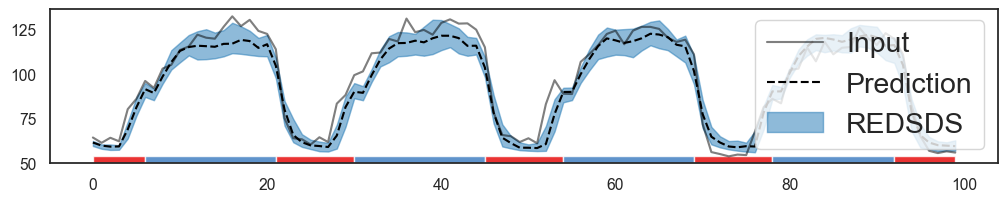
\includegraphics[width=0.49\linewidth]{changepoints/figs/e-prob.png}
    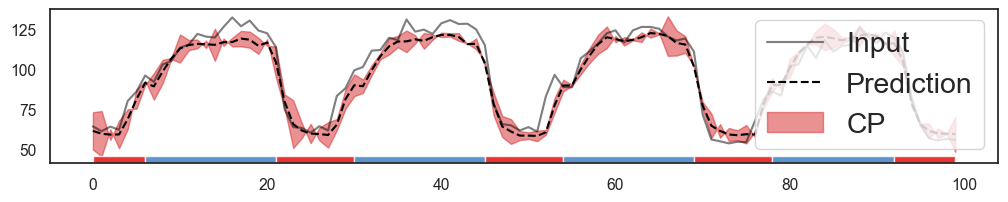
\includegraphics[width=0.49\linewidth]{changepoints/figs/e-cp.png}
    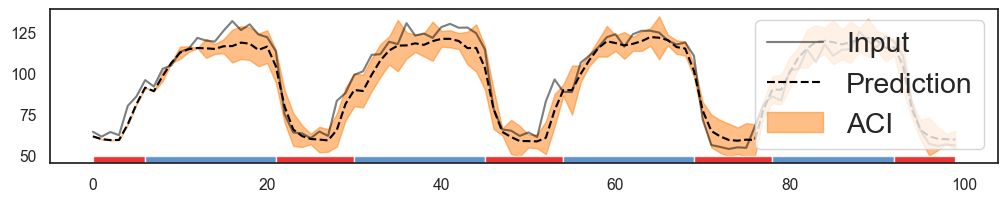
\includegraphics[width=0.49\linewidth]{changepoints/figs/e-aci.png}
    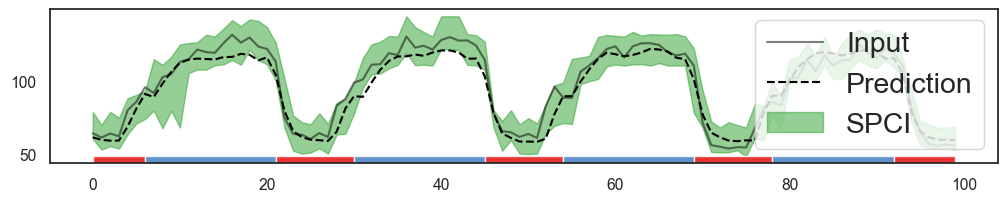
\includegraphics[width=0.49\linewidth]{changepoints/figs/e-spci.png}
    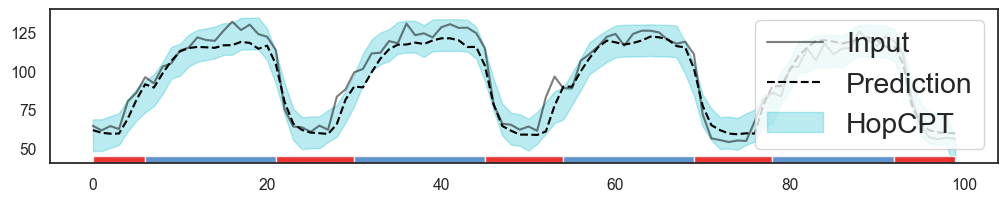
\includegraphics[width=0.49\linewidth]{changepoints/figs/e-hop.png}
    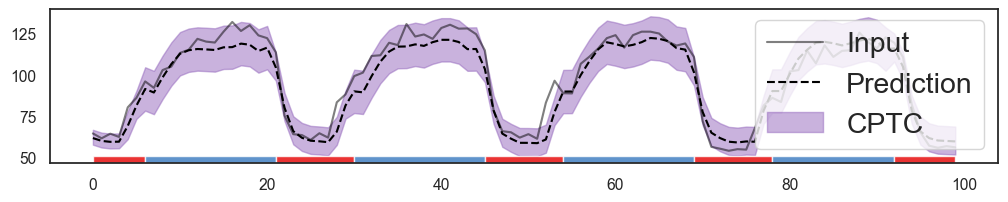
\includegraphics[width=0.49\linewidth]{changepoints/figs/e-ours.png}
    \vspace{-0.5em}
    \caption{\textbf{Visualization of prediction intervals on the Electricity hourly demand dataset.} The red and blue bars in the bottom reflects the underlying switching state of day and night. Our method (purple) adapts to different levels of volatility between day and night, and achieves stabler coverage over time, whereas ACI (yellow) over-covers during the night and under-covers at change points.}
    \label{fig:demonstration}
\vspace{-1em}
\end{figure}


 
%\sofi{Some more visualizations}
%\subsection{Ablation study on aggreagation methods} 
%\sofi{Ablation study on aggreagation methods, ablation on sequence length?}

\vspace{-0.6em}
\subsection{Ablation Studies}
\label{sec:accuracy}
\vspace{-0.5em}
\paragraph{Robustness to $p(\hat{z})$ accuracy.} We conduct ablation studies on the 3 synthetic datasets of which we have ground truth underlying states. As shown in table \ref{tab:z_exp}, it is evident that increasing the error in the state prediction does not affect the coverage performance. This verifies the robustness of our algorithm and theoretical results (Theorem \ref{thm:asymptotic_validity} and \ref{thm:imperfect_state_predictions}). Table \ref{tab:z_exp_area} further shows that the error of state prediction reflects on the width of the prediction intervals: while remaining the same level of coverage, the better the state predictions, the sharper the intervals.

\vspace{-1.5em}
\begin{minipage}{0.58\textwidth}
\begin{table}[H]
    \caption{Coverage of CPTC for using ground truth (GT) labels and with various levels of injected noise, on synthetic data with $T=200$. We can see that coverage performance does not change significantly with error in state prediction. }   
    \vspace{0.4em}
    \label{tab:z_exp}
    \centering
    \resizebox{\textwidth}{!}{%
    \begin{tabular}{c|c c c}
        \toprule
        & Ground truth state labels & GT w/ $20\%$ error & GT w/ $50\%$ error \\ 
        \midrule
        BB obs.  & 90.31 \plusminus 1.27 & 90.27 \plusminus 1.30 & 90.13 \plusminus 1.40 \\ 
        BB dyn.  & 90.34 \plusminus 0.93 & 90.32 \plusminus 0.96 & 90.33 \plusminus 1.05 \\ 
        3-mode  & 92.67 \plusminus 1.52 &  92.70 \plusminus 1.63  & 92.53 \plusminus 1.54 \\ 
        \bottomrule
    \end{tabular}
    }
\end{table}

\end{minipage}
\hfill
\begin{minipage}{0.38\textwidth}
\begin{table}[H]
    \centering
    \caption{Interval width under the same setting. While the coverage guarantee is the same, the more accurate the state prediction is, the sharper the intervals.}
    \vspace{0.4em}
    \label{tab:z_exp_area}
    \resizebox{\textwidth}{!}{%
    \begin{tabular}{c| c c c}
        \toprule
        & GT & w/ $20\%$ err & w/ $50\%$ err\\ 
        \midrule
        BB obs. & 3.61 \plusminus 0.93 & 3.75 \plusminus 0.99 & 3.94 \plusminus 1.17 \\ 
        BB dyn. & 2.09 \plusminus 0.60 & 2.15 \plusminus 0.62 & 2.18 \plusminus 0.65 \\ 
        3-mode & 2.04 \plusminus 0.67 &  2.19 \plusminus 0.76  & 2.27 \plusminus 0.89 \\ 
        \bottomrule
    \end{tabular}
    }       
\end{table}
\end{minipage}

\vspace{0.5em}
Additional ablation studies are presented in Appendix \ref{app:more_experiments}. On \textbf{Aggregation Methods} (by discretization as \Eqref{eq:aggregation-average} or union as \Eqref{eq:aggregation-union}), we found that on our benchmark datasets, union is a close proximation of the true objective, and CPTC achieves similar width and coverage on a sampled subset. For \textbf{Long Horizon Forecasting} where $T \geq 10,000$, our method still achieves valid and stable coverage, but have wider PI width compared to SPCI an HopCPT. They achieve this by frequently re-training their models online, which CPTC does not and is less computationally demanding.

\section{Conclusion and Discussion}

In this paper, we introduced Conformal Prediction for Time-series with Change points (CPTC), a novel conformal prediction algorithm for uncertainty quantification in non-stationary time series. By leveraging state information in switching dynamics systems models, CPTC offers improvements in adaptivity over existing conformal prediction methods. Our theoretical guarantees ensure validity \textit{without assumptions} on time-series stationarity or accurate
state predictions. Empirical results corroborate our theory and demonstrate the effectiveness of CPTC across diverse synthetic and real-world datasets, achieving robust coverage under distributional shifts with comparable sharpness compared to state-of-the-art baselines. The adaptivity advantage is most pronounced in shorter time series, when baselines require more data to react or learn temporal correlations. %CPTC as a versatile tool for time-series UQ in dynamic and complex environments. 
% achieving robust coverage under distributional shifts with comparable sharpness. The adaptivity advantage is  especially on medium-length time series.  while empirical results demonstrate the effectiveness of CPTC across diverse synthetic and real-world datasets. 

Limitations of CPTC include (1) slower convergence rate in scenarios with frequent or unpredictable state transitions, as the algorithm requires sufficient observations within each state to achieve optimal calibration and sharpness, (2) wider prediction interval width when applied to very long time series compared methods specialized for such scenarios (e.g. HopCPT), and (3) requirement of a state prediction model, making our method primarily applicable to SDS models and discrete SSMs. Future work could explore extending the framework to continuous states and the theoretical implications thereof, and studying the decision theoretic properties of using conformal prediction for safety-critical applications requiring real-time adaptation.

%\section*{Acknowledgement}

% \clearpage

% \section*{Acknowledgments and Disclosure of Funding}

% This work was supported in part by the U.S. Army Research Office under Army-ECASE award W911NF-07-R-0003-03, the U.S. Department Of Energy, Office of Science, IARPA HAYSTAC Program, NSF Grants SCALE MoDL-2134209, CCF-2112665 (TILOS), \#2205093, \#2146343, and \#2134274, as well as CDC-RFA-FT-23-0069 from the CDC's Center for Forecasting and Outbreak Analytics. 

% \bibliography{ref.bib}
% \bibliographystyle{abbrv}

% \appendix
\section{Appendix}
\clearpage
\onecolumn

\section{Theoretical Results and Proofs}
\label{app:proofs}

\subsection{Setup and Notation}

Let \( z_t \in \mathcal{Z} = \{1, \dots, K\} \) denote the unobserved discrete mode,  \( x_t \in \mathcal{X} \) denote the continuous state, and \( y_t \in \mathcal{Y} \) the observation at time $t$. We assume we have access to a probabilistic model \( \hat{p}(z_t | X_{1:t-1}) \) that estimates the mode $\hat{z}_t$.

For a target coverage rate \( 1 - \alpha \), let \( \Gamma_{t}(X_t) \) be the prediction set at time \( t \). We define the miscoverage indicator \( M_t \) as follows, and aim to bound the overall miscoverage rate over \( T \) time steps:
\[
M_t = \frac{1}{T} \sum_{t=1}^T err_t, \quad \text{where} \quad err_t := \mathbbm{1}\big(Y_t \notin \Gamma_{t}(X_t)\big),
\]



\subsection{Proofs: Lemma}

In practical scenarios, the state prediction model may not be perfectly accurate. We now analyze the impact of imperfect state predictions on the coverage guarantees of the CPTC algorithm.
 
We derive the following lemma from the convergence result of Proposition 4.1 in \cite{gibbs2021adaptive} with two additional assumptions also according to \cite{gibbs2021adaptive}: (1) the existence of a single fixed optimal target $a^* \in [0,1]$, and (2) $\mathbb{E} [err_t | a_t] = M(a_t)$. These are reasonable assumptions that allow us to quantify distribution shifts and are necessary for analyzing adaptation behavior  (whereas proposition 4.1 itself is a worst-case upper bound.) We refer the readers to the original paper for the complete derivation. 


\begin{lemma}[Adaptive Conformal Inference Miscoverage Bound Within Predicted States]\label{lemma:aci_within_states} Let \( \mathcal{T}_z = \{ t \in \{1, \dots, T\} : \hat{z}_t = z \} \) denote the set of times when the predicted state is \( z \). For any \( T > 1 \) and predicted state \( \hat{z}_t = z \), the Adaptive Conformal Inference (ACI) algorithm ensures that there exists a constant \( \delta_{z, T} \) such that:
 \[ 
\left| \frac{1}{|\mathcal{T}_z|} \sum_{t \in \mathcal{T}_z} \mathbb{E}[err_t] - \alpha \right| \leq \delta_{z, T}
\]

Explicitly, 
\[
\delta_{z,T} =  \frac{1 - (1-c\gamma)^{|\mathcal{T}_z|}}{|\mathcal{T}_z| \gamma} |\alpha - \alpha^{*}_z|
\]
where 
\begin{itemize}
    \item  $\alpha^*_z$ is the optimal miscoverage target for timesteps $\mathcal{T}_z$.
    \item $\gamma$ is the step size
    \item $c$ the miscoverage constant.
\end{itemize}  Note that $\delta_{z,T}$ decays at a rate of $\mathcal{O}(T)$ and satisfies
$ \lim_{\mathcal{T}_z \to \infty} \delta_{z,T} = 0$.

\end{lemma}

\subsection{Proof of Theorem \ref{thm:asymptotic_validity}}

\begin{theorem*}[
\ref{thm:asymptotic_validity} Asymptotic validity of CPTC ]
For any sample size \( T \geq 1 \), without placing any assumptions, the CPTC algorithm ensures that:
\[  
\left| \frac{1}{T} \sum_{t=1}^T \mathbb{E}[err_t] - \alpha \right| \leq \frac{1}{T} \sum_{z=1}^K    |\mathcal{T}_z | \delta_{z,T}  = \frac{1}{T} \sum_{z=1}^K  \frac{ 1 - (1-c\gamma)^{|\mathcal{T}_z|}  }{\gamma} |\alpha - \alpha^{*}_z|
\]
which decays at a rate of $\mathcal{O}(T)$ and satisfies
 \[
 \lim_{T \to \infty} \left| \frac{1}{T} \sum_{t=1}^T \mathbb{E}[err_t] - \alpha \right|= 0.
 \]
\end{theorem*}

To prove theorem \ref{thm:asymptotic_validity}, we assume that both the distribution of the underlying modes $z$ and the predictions $\hat{z}$ is stationary (Assumption \ref{assump:stationary_distribution}). 

\begin{assumption}[Stationary Distribution of States]\label{assump:stationary_distribution}
The sequence of true states \( \{z_t\} \) has a stationary distribution \( \pi(z) \), and the sequence of predicted states \( \{\hat{z}_t\} \) also has a stationary distribution \( \hat{\pi}(z) \). Specifically:
\[
\forall z, \in \mathcal{Z}, \quad \lim_{t \to \infty} p(z_t = z) = \pi(z), \quad \lim_{t \to \infty} p(\hat{z}_t = z) = \hat{\pi}(z),
\]
\end{assumption}


This assumption is well-justified in practical scenarios where the sequence of observations and predictions arises from processes that, while non-stationary over short intervals, exhibit stable long-term behavior. In time-series or dynamic environments, regularities in data generation or prediction models often lead to empirically observed stationarity in distributions. While restrictive, this assumption aligns with prior work in sequential and online prediction frameworks, where stationarity assumptions are standard to derive theoretical guarantees.

 
\begin{proof}[Proof of Theorem \ref{thm:asymptotic_validity}]
Let \( \mathcal{T}_z = \{ t \in \{1, \dots, T\} : \hat{z}_t = z \} \) represent the set of timesteps when the predicted state is \( z \). For the total number of timesteps \( T \), the overall miscoverage error can be expressed as:
\begin{align*}
\frac{1}{T} \sum_{t=1}^T \mathbb{E}[err_t] & = \frac{1}{T} \sum_{z=1}^K \sum_{t \in \mathcal{T}_z} \mathbb{E}[err_t]\\
&= \frac{1}{T} \sum_{z=1}^K |\mathcal{T}_z| \left( \frac{1}{|\mathcal{T}_z|} \sum_{t \in \mathcal{T}_z} \mathbb{E}[err_t] \right).
\end{align*}

From Lemma \ref{lemma:aci_within_states}, for any predicted state \( z \), the miscoverage within \( \mathcal{T}_z \) satisfies:
\[
\left| \frac{1}{|\mathcal{T}_z|} \sum_{t \in \mathcal{T}_z} \mathbb{E}[err_t] - \alpha \right| \leq \delta_{z,T},
\]
where:
\[
\delta_{z,T} = \frac{1 - (1-c\gamma)^{|\mathcal{T}_z|}}{|\mathcal{T}_z| \gamma} |\alpha - \alpha^{*}_z|.
\]

Substituting this bound into the overall miscoverage error, we obtain:
\[
\left| \frac{1}{T} \sum_{t=1}^T \mathbb{E}[err_t] - \alpha \right| \leq \frac{1}{T} \sum_{z=1}^K |\mathcal{T}_z| \delta_{z,T}.
\]

Expanding \( \delta_{z,T} \), the overall bound becomes:
\[
\left| \frac{1}{T} \sum_{t=1}^T \mathbb{E}[err_t] - \alpha \right| \leq \frac{1}{T} \sum_{z=1}^K \frac{ 1 - (1-c\gamma)^{|\mathcal{T}_z|}}{\gamma} |\alpha - \alpha^{*}_z|.
\]

By assumption \ref{assump:stationary_distribution}, as \( T \to \infty \), the size of \( |\mathcal{T}_z| \) for each state \( z \) grows proportionally to \( T \). The term \( 1 - (1-c\gamma)^{|\mathcal{T}_z|} \) approaches \( 1 \), while \( |\mathcal{T}_z| / T \) converges to the relative proportion of time spent in state \( z \), denoted as \( p_z \). Hence, as \( T \to \infty \), the overall bound \(
\left| \frac{1}{T} \sum_{t=1}^T \mathbb{E}[err_t] - \alpha \right| \to  0\).

Thus, the CPTC algorithm ensures that the overall error converges to the target coverage level \( \alpha \) at a rate of \( \mathcal{O}(T) \), satisfying:
\[
\lim_{T \to \infty} \left| \frac{1}{T} \sum_{t=1}^T \mathbb{E}[err_t] - \alpha \right| = 0.
\]
\end{proof}



\subsection{Proof of Theorem \ref{thm:imperfect_state_predictions}}
\begin{theorem*}[
\ref{thm:imperfect_state_predictions} Finite-Sample Miscoverage Bound with Imperfect State Predictions] 
For any sample size \( T \geq 1 \), the CPTC algorithm ensures that:
\[
\left| \frac{1}{T} \sum_{t=1}^{T} \mathbb{E}[err_t]  - \alpha \right| \leq \epsilon \cdot \max_z \delta_{z,T}
\]
where:
\begin{itemize}
    \item \(err_t := \mathbbm{1}\big(Y_t \notin \Gamma_{t}(X_t)\big)\), the miscoverage rate. 
    \item \( \mathcal{T}_z = \{ t \in \{1, \dots, T\} : \hat{z}_t = z \} \), the set of times when the predicted state is \( z \).
    %\item \( z_t \) denotes the true latent state at time \( t \), and \( \hat{z}_t \) the predicted state. 
    \item \( \epsilon = \mathbb{P}(\hat{z}_t \neq z_t) \) is the misclassification rate of the state predictions.
    \item \( \delta_{z,T} \) is the deviation from \( \alpha \) within any predicted state $z$ as in  Lemma \ref{lemma:aci_within_states}. %, which satisfies \( \delta_T \to 0 \) as \( |\mathcal{T}_z| \to \infty \).
\end{itemize}
\end{theorem*}

 

\begin{proof}[Proof of Theorem \ref{thm:imperfect_state_predictions}]

First we will partition time into correct vs.\ incorrect predictions. Define:
\[
  \mathcal{C} 
  \;=\; \{\,t : \hat{z}_t = z_t\},
  \quad
  \mathcal{I} 
  \;=\; \{\,t : \hat{z}_t \neq z_t\},
  \quad
  \text{and}
  \quad
  \frac{|\mathcal{I}|}{T} \;=\;\epsilon.
\]

\smallskip

\textbf{Calibrated expected coverage on correctly predicted states \(\mathcal{C}\).}
Since there are no distribution shifts within each state, we have the same expected error from calibration data. Therefore,
\[
  \mathbb{E}[\mathrm{err}_t] 
  \;=\; \alpha
  \quad\Longrightarrow\quad
  \mathbb{E}[\mathrm{err}_t] - \alpha 
  \;=\; 0.
\]

\smallskip

\textbf{Bounded deviation on incorrectly predicted states \(\mathcal{I}\).}
On \(\mathcal{I}\), we have 
\(\bigl|\mathbb{E}[\mathrm{err}_t] - \alpha\bigr| \le \delta_{z,T}\).  
Therefore,
\[
  \sum_{t=1}^T 
    \bigl|\mathbb{E}[\mathrm{err}_t] - \alpha\bigr|
  \;=\;
  \sum_{t \in \mathcal{C}} \bigl|\mathbb{E}[\mathrm{err}_t] - \alpha\bigr|
  \;+\;\;
  \sum_{t \in \mathcal{I}} \bigl|\mathbb{E}[\mathrm{err}_t] - \alpha\bigr|
  \;\;\le\;\;
  0 \;+\; |\mathcal{I}|\;\delta_{z,T}
  \;=\; 
  |\mathcal{I}|\;\delta_{z,T}.
\]
Since \(\tfrac{|\mathcal{I}|}{T}=\epsilon\), dividing by \(T\) yields
\[
  \frac{1}{T} 
  \sum_{t=1}^T 
    \bigl|\mathbb{E}[\mathrm{err}_t] - \alpha\bigr|
  \;\;\le\;\;
  \epsilon\,\delta_{z,T}.
\]

\smallskip

\textbf{Combine to achieve the overall bound.}
By the triangle inequality, we know that
\[
  \left|
    \frac{1}{T}\sum_{t=1}^T \mathbb{E}[\mathrm{err}_t] - \alpha
  \right|
  \;\;\le\;\;
  \frac{1}{T}\sum_{t=1}^T 
    \bigl|\mathbb{E}[\mathrm{err}_t] - \alpha\bigr|.
\]
Hence, from the previous step,
\[
  \left|
    \frac{1}{T}\sum_{t=1}^T \mathbb{E}[\mathrm{err}_t] - \alpha
  \right|
  \;\;\le\;\;
  \epsilon\,\delta_{z,T}.
\]
Since on \(\mathcal{I}\) the predicted state \(\hat{z}_t\) could vary among different \(z\) values, we take
\(\delta_{z,T} \le \max_{z}\,\delta_{z,T}\). 
Thus,
\[
  \left|
    \frac{1}{T}\sum_{t=1}^T \mathbb{E}[\mathrm{err}_t] - \alpha
  \right|
  \;\;\le\;\;
  \epsilon\,\max_{z}\,\delta_{z,T}.
\]
\end{proof}

% ------------------
% corollaries 
% ------------------
\subsection{Corollaries}

Theorem \ref{thm:imperfect_state_predictions} indicates that the overall miscoverage rate deviates from the desired level \( \alpha \) by at most \( \epsilon \cdot \max_z \delta_{z,T} \). The misclassifications rate \( \epsilon \) contributes directly to the deviation, and the calibration error \( \delta_{z,T} \) within each predicted state decreases as more data becomes available. As \( T \) increases and \( \max_z \delta_{z,T} \to 0 \), the deviation is primarily governed by the misclassification rate \( \epsilon \). 

\vspace{0.5em}
\begin{corollary}[Zero miscoverage rate under Accurate State Prediction]
 If predicted state probabilities are accurate \( \hat{p}(z_t | x_{1:t-1}) = p(z_t | x_{1:t-1}) \), then \( \epsilon = 0 \), therefore $\mathbb{E}[err_t] = \alpha$ for all $T$, achieving optimal performance of online conformal prediction. 
\end{corollary}

\vspace{0.5em}

\begin{corollary}[Asymptotic calibration under eventually correct  State Prediction]
If the predicted state probabilities \( \hat{p}(z_t | x_{1:t-1}) \) converge in probability to the true state distribution \( p(z_t | x_{1:t-1}) \) as \( T \to \infty \). With \( T \to 0\), \( \epsilon \to 0 \) as well. Hence, the overall miscoverage rate converges asymptotically to 0.
\end{corollary}

\subsection{Proof of Theorem \ref{thm:adaptation}}

Consider a data stream with a distribution shift occurring at time $t_{{\text{shift}}}$. Let $\alpha^*_{j}$ denote the optimal target error rate for mode $j$ after the shift, and assume that the predicted state $\hat{z}_t$ correctly reflects the shift: $t_{\text{shift}}$ and $\alpha^*_{z} = \alpha^*_{j}$ for $t > t_{{\text{shift}}}$. For conciseness of notation in Theorem \ref{thm:adaptation}, let $\delta_{j,T}$ and $\delta_{ACI,T}$ denote the miscoverage rate \textit{starting from } $t_{\text{shift}}$ for CPTC and ACI respectively.


\begin{theorem*}[\ref{thm:adaptation}
Miscoverage Ratio under State-Coincident Distribution Shift]
Under a state shift from $i$ to $j$ at time step $t_{\text{shift}}$, coinciding with predicted transition, the CPTC algorithm achieves faster convergence to the new target $\alpha^*_{j}$ compared to non-state-aware algorithm ACI at a ratio of:
\[
\frac{\delta_{j,T}}{\delta_{\text{ACI},T}} \leq \frac{|\alpha_{j, t_{\text{shift}}-1}  - \alpha^{*}_{j}|}{|\alpha_{ t_{\text{shift}}-1} - \alpha^{*}_{j}|}
\]
\end{theorem*}

\begin{proof}[Proof of Theorem \ref{thm:adaptation}]

We want to compare the convergence behavior of CPTC and a non-segmented online conformal prediction algorithm (e.g., ACI) when a distribution shift occurs at time $t_{\text{shift}}$ and this shift coincides with a predicted state transition from $i$ to $j$. 

We assume that State prediction coincident shift, meaning $\alpha_z^* = \alpha_i^*$ for $t\leq t_{\text{shift}}$ and $\alpha_z^* = \alpha^*_j$ for $t> t_{\text{shift}}$.


From Lemma \ref{lemma:aci_within_states} and Theorem \ref{thm:asymptotic_validity}, we have bounds on these deviations. Taking the ratio of the bounds, we have:

\[
\frac{\delta_{j,T}}{\delta_{\text{ACI},T}} \leq \frac{c \cdot \frac{1}{\gamma} |\alpha_{j, t_{\text{shift}}-1}  - \alpha^{*}_{j}|}{c \cdot \frac{1}{\gamma} |\alpha_{ t_{\text{shift}}-1} - \alpha^{*}_{j}|} =  \frac{|\alpha_{j, t_{\text{shift}}-1}  - \alpha^{*}_{j}|}{|\alpha_{ t_{\text{shift}}-1} - \alpha^{*}_{j}|}
\]

%However, we need to account for the fact that CPTC is only updating on the steps where state $j$ is predicted. Since $|\mathcal{T}_j|$ is the number of steps in state $j$ up to time $T$, the proportion of updates is $\frac{|\mathcal{T}_j|}{T}$. Incorporating this, we get:

\end{proof}

We elaborate on the implication of this result. The ratio indicates that the CPTC achieves lower miscoverage rate when the initial target $\alpha_{j, t_{\text{shift}}-1}$ for state $j$ in CPTC is closer to the new optimal target $\alpha^*_j$ than the global target $\alpha_{t_{\text{shift}}-1}$ used by ACI. This is because CPTC maintains separate targets for each state, allowing it to better track state-specific optimal targets. The base model takes around 2 hours of training time on the GPU 




% \subsection{Proof of }

% \begin{proof}
    

% 1.  \textbf{Law of Total Probability:} We can decompose the overall coverage probability using the law of total probability, conditioning on the true state \(z_t\):

%     \begin{equation}
%     P(y_t \in \Gamma_t(x_t)) = \sum_{z \in Z} P(y_t \in \Gamma_t(x_t) | z_t = z) P(z_t = z)
%     \end{equation}

% 2.  \textbf{Union Bound:} Since \(\Gamma_t(x_t)\) is the union of \(\Gamma_{z,t}(x_t)\) over all states, if \(y_t\) belongs to any \(\Gamma_{z,t}(x_t)\), it must also belong to \(\Gamma_t(x_t)\). Therefore, for any state \(z\):

%     \begin{equation}
%     P(y_t \in \Gamma_t(x_t) | z_t = z) \geq P(y_t \in \Gamma_{z,t}(x_t) | z_t = z)
%     \end{equation}

% 3.  \textbf{Conditional Coverage:} By assumption, each individual prediction set \(\Gamma_{z,t}(x_t)\) has conditional coverage of at least \(1 - \alpha_{z,t}\) given state \(z\). Thus:

%     \begin{equation}
%     P(y_t \in \Gamma_{z,t}(x_t) | z_t = z) \geq 1 - \alpha_{z,t}
%     \end{equation}

% 4.  \textbf{Combining Steps:} Substituting steps 2 and 3 into step 1, we get:

%     \begin{equation}
%     P(y_t \in \Gamma_t(x_t)) \geq \sum_{z \in Z} (1 - \alpha_{z,t}) P(z_t = z)
%     \end{equation}

%     This can be rewritten as:

%     \begin{equation}
%      P(y_t \in \Gamma_t(x_t)) \geq 1 - \sum_{z \in Z} \alpha_{z,t} P(z_t = z)
%     \end{equation}

% 5.  \textbf{Long-run average of \(\alpha_{z,t}\):} Taking expectation with respect to the predicted state, we have:
%      \begin{equation}
%      \mathbb{E}_{z_t \sim \hat{p}(z_t|x_{t-1}, z_{1:t-1})} [\sum_{z \in Z} \alpha_{z,t} P(z_t = z)]
%      = \mathbb{E}_{z \sim \hat{p}(z|x_{t-1}, z_{1:t-1})} [\alpha_{z,t}]
%      \end{equation}
%     Taking the long-run average, we have:
%     \begin{equation}
%      \lim_{T \to \infty} (1/T) \sum_{t=1}^{T} \mathbb{E}_{z \sim \hat{p}(z|x_{t-1}, z_{1:t-1})} [\alpha_{z,t}]
%      = \lim_{T \to \infty} (1/T) \sum_{z \in Z} \sum_{t=1}^{T} \alpha_{z,t}
%      = \lim_{T \to \infty} \sum_{z \in Z} (T_z/T)(1/T_z) \sum_{t=1}^{T_z} \alpha_{z,t}
%      \leq \sum_{z \in Z} (T_z/T)\alpha = \alpha
%      \end{equation}
     
%     By assumption 2, we know that the long term average of \(\alpha_{z,t}\) is less than or equal to \(\alpha\). Thus, we have:
%     \begin{equation}
%     P(y_t \in \Gamma_t(x_t)) \geq 1 - \alpha
%     \end{equation}

% \textbf{Conclusion of Proof:}

% The union operation ensures that the overall prediction set \(\Gamma_t(x_t)\) achieves a coverage probability of at least \(1 - \alpha\), provided that each individual state-specific prediction set \(\Gamma_{z,t}(x_t)\) satisfies the conditional coverage guarantee and the long-run average of the state-specific \(\alpha_{z,t}\) converges to a value less than or equal to \(\alpha\). This guarantee holds even though the algorithm might exhibit over-coverage in practice.

% \end{proof}

%----------------------------------------------------------


% \newpage
% \section{Old Proofs}



% For theoretical analysis we make the following assumptions.

% \begin{assumption}[Stationary Distribution of States]\label{assump:stationary_distribution}
% The sequence \( \{z_t\} \) has a stationary distribution \( \pi(z) \), such that:
% \[
% \lim_{t \to \infty} p(z_t = z) = \pi(z), \quad \forall z \in \mathcal{Z}.
% \]
% \end{assumption}

% \begin{assumption}[Bounded Transition Probabilities]\label{assump:bounded_transition}
% There exists a constant \( \gamma > 0 \) such that the transition probabilities between states satisfy:
% \[
% p(z_{t+1} = z' \mid z_t = z, x_{1:t}) \leq \gamma, \quad \forall z, z' \in \mathcal{Z}.
% \]
% \end{assumption}

% \subsection{Group-wise Coverage with State Prediction converging to True Distribution}
% \label{appendix:asymptotic_state_proof}

% \begin{assumption}[Latent State Model]\label{assump:latent_state_model}
% The latent state \( z_t \) follows a Switching Dynamical System (SDS) model with \( K \) possible states, and transitions according to the conditional probabilities \( p(z_t | X_{1:t-1}) \).
% \end{assumption}

% \begin{theorem}[Asymptotic Group-Wise Coverage]\label{thm:group_wise_coverage}
% Let \( X_t \in \mathcal{X} \) and \( Y_t \in \mathcal{Y} \) be as defined. Under Assumptions \ref{assump:latent_state_model} and \ref{assump:accurate_state_prediction}, for a desired confidence level \( 1 - \alpha \), Algorithm \ref{alg:cptc} constructs prediction sets \( \Gamma_{1 - \alpha}(X_t) \)  that achieve asymptotic group-wise coverage:
% \[
% \lim_{T \to \infty} \mathbb{P}\big(Y_t \in \Gamma_{1 - \alpha}(X_t) \mid z_t = k\big) = 1 - \alpha, \quad \forall k \in \mathcal{Z}.
% \]
% \end{theorem}

% \begin{proof}
% Under Assumption \ref{assump:accurate_state_prediction}, the predicted state probabilities \( \hat{p}(z_t | X_{1:t-1}) \) converge in probability to the true state probabilities \( p(z_t | X_{1:t-1}) \) as \( T \to \infty \):

% \begin{equation}\label{eq:state_prob_convergence}
% \hat{p}(z_t | X_{1:t-1}) \xrightarrow{P} p(z_t | X_{1:t-1}).
% \end{equation}


% Let \( \hat{z}_t \) be the state sampled from \( \hat{p}(z_t | X_{1:t-1}) \), and \( z_t \) be the true state sampled from \( p(z_t | X_{1:t-1}) \). From \eqref{eq:state_prob_convergence}, the total variation distance between \( \hat{p}(z_t | X_{1:t-1}) \) and \( p(z_t | X_{1:t-1}) \) converges to zero. Therefore, the probability that \( \hat{z}_t = z_t \) converges to one:

% \begin{equation}\label{eq:state_convergence}
% \lim_{T \to \infty} \mathbb{P}(\hat{z}_t = z_t) = 1.
% \end{equation}


% Algorithm \ref{alg:cptc} updates the miscoverage levels \( \alpha_{z,t} \) using the rule:

% \begin{equation}\label{eq:alpha_update}
% \alpha_{\hat{z}_t,t+1} = \alpha_{\hat{z}_t,t} + \gamma \left( \alpha - \mathbbm{1}\{ Y_t \notin \Gamma_t(X_t) \} \right),  
% \end{equation}

% where \( \gamma \) is the learning rate (\( \gamma > 0 \) and small), and \( \mathbbm{1}\{ Y_t \notin \Gamma_t(X_t) \} \) is the indicator function for miscoverage at time \( t \). Without loss of generality, we focus on the updates conditioned on \( z_t = k \). From \eqref{eq:state_convergence}, updates to \( \alpha_{k,t} \) occur predominantly when \( \hat{z}_t = z_t = k \). 

% Define the conditional miscoverage rate \( e_k(\alpha_{k,t}) \) as:

% \begin{equation}\label{eq:ek_definition}
% e_k(\alpha_{k,t}) = \mathbb{P}\left( Y_t \notin \Gamma_t(X_t) \mid z_t = k, \alpha_{k,t} \right).
% \end{equation}

% Taking the expectation of \eqref{eq:alpha_update} conditioned on \( z_t = k \) and \( \alpha_{k,t} \), we obtain:

% \begin{equation}\label{eq:expected_alpha_update}
% \mathbb{E}\left[ \alpha_{k,t+1} \mid \alpha_{k,t}, z_t = k \right] = \alpha_{k,t} + \gamma \left( \alpha - e_k(\alpha_{k,t}) \right).
% \end{equation}

% By the Robbins-Monro algorithm in stochastic approximation theory \citep{robbins1951stochastic}, the sequence \( \{\alpha_{k,t}\} \) converges almost surely to the equilibrium point \( \alpha_k^\ast \) satisfying:

% \begin{equation}\label{eq:fixed_point}
% e_k(\alpha_k^\ast) = \alpha.
% \end{equation}


% Similar results are proved in \cite{gibbs2021adaptive}.  As \( T \to \infty \), from \eqref{eq:state_prob_convergence} and the convergence of \( \alpha_{k,t} \) to \( \alpha_k^\ast \), we have:

% \begin{equation}\label{eq:adjusted_alpha_convergence}
% \hat{\alpha}_{k,t} \xrightarrow{P} \alpha_k^\ast \cdot p(z_t = k | X_{1:t-1}).
% \end{equation}

% Since the conformal prediction sets are calibrated using \( \hat{\alpha}_{k,t} \) and the nonconformity scores \( \mathcal{S}_k \) specific to state \( k \), the miscoverage rate conditioned on \( z_t = k \) converges to \( \alpha \):

% \begin{equation}\label{eq:group_wise_miscoverage}
% \lim_{T \to \infty} \mathbb{P}\left( Y_t \notin \Gamma_t(X_t) \mid z_t = k \right) = e_k(\alpha_k^\ast) = \alpha.
% \end{equation}

% Here, \( \Gamma_t(X_t) = \bigcup_{z \in \mathcal{Z}} \Gamma_{z,t}(X_t) \), ensuring that the overall prediction set includes the contributions from all states. Therefore, the coverage conditioned on \( z_t = k \) satisfies:

% \[
% \lim_{T \to \infty} \mathbb{P}\left( Y_t \in \Gamma_t(X_t) \mid z_t = k \right) = 1 - \alpha.
% \]

% This establishes that Algorithm \ref{alg:cptc} achieves asymptotic group-wise coverage for each state \( k \in \mathcal{Z} \), as desired.

% \end{proof}

% \begin{lemma}[Bounded Conditional Miscoverage Variance]\label{lem:bounded_variance}
% Under the asymptotic conditional coverage guarantee for each state \( z \in \mathcal{Z} \), the variance of the miscoverage indicator \( M_t \) conditioned on \( z_t = z \) is bounded:
% \[
% \operatorname{Var}\big(M_t \mid z_t = z\big) \leq \alpha(1 - \alpha).
% \]
% \end{lemma}

% \begin{proof}
% Given that \( M_t \) is an indicator variable for miscoverage conditioned on \( z_t = z \), and from Theorem \ref{thm:group_wise_coverage} we have:
% \[
% \lim_{T \to \infty} \mathbb{E}\big[M_t \mid z_t = z\big] = \alpha.
% \]
% Since \( M_t \in \{0, 1\} \), it follows that:
% \[
% \operatorname{Var}\big(M_t \mid z_t = z\big) = \mathbb{E}\big[M_t^2 \mid z_t = z\big] - \left(\mathbb{E}\big[M_t \mid z_t = z\big]\right)^2 =  \alpha(1 - \alpha).
% \]
% \end{proof}

% \subsection{Overall Miscoverage Bound}
% \label{appendix:overall_asymptotic_coverage}


% \begin{assumption}[Bounded Transition Probabilities]\label{assump:bounded_transition}
% There exists a constant \( \delta > 0 \) such that the transition probabilities between states satisfy:
% \[
% p(z_{t+1} = z' \mid z_t = z, X_{1:t}) \leq \delta, \quad \forall z, z' \in \mathcal{Z}.
% \]
% \end{assumption}

% \begin{assumption}[Stationary Distribution of States]\label{assump:stationary_distribution}
% The sequence \( \{z_t\} \) has a stationary distribution \( \pi(z) \), such that:
% \[
% \lim_{t \to \infty} p(z_t = z) = \pi(z), \quad \forall z \in \mathcal{Z}.
% \]
% \end{assumption}

% \begin{theorem}[Overall Miscoverage Bound]\label{thm:overall_miscoverage}
% Under Assumptions \ref{assump:bounded_transition} and \ref{assump:stationary_distribution}, and using the result from Lemma \ref{lem:bounded_variance}, the overall miscoverage rate satisfies:
% \[
% \lim_{T \to \infty} \mathbb{P}\big(Y_t \in \Gamma_{1 - \alpha}(X_t) \big) = 1 - \alpha.
% \]
% \end{theorem}

% \begin{proof}
% We aim to apply a concentration inequality to \( \{M_t\} \). By the law of total variance:
% \[
% \operatorname{Var}(M_t) = \operatorname{Var}\big( \mathbb{E}[M_t \mid z_t] \big) + \mathbb{E}\big( \operatorname{Var}(M_t \mid z_t) \big).
% \]
% From Lemma \ref{lem:bounded_variance}, we have:
% \[
% \operatorname{Var}\big(M_t \mid z_t = z\big) \leq \alpha(1 - \alpha), \quad \forall z \in \mathcal{Z}.
% \]
% Since \( \lim_{T \to \infty} \mathbb{E}[M_t \mid z_t = z] = \alpha \) for all \( z \), the variance \( \operatorname{Var}\big( \mathbb{E}[M_t \mid z_t] \big) \) becomes negligible as \( T \to \infty \).

% Therefore, the total variance of \( M_t \) is bounded:
% \[
% \operatorname{Var}(M_t) \leq \alpha(1 - \alpha).
% \]

% The sequence \( \{M_t\} \) can be considered as a martingale difference sequence with bounded differences. Specifically, \( |M_t - \mathbb{E}[M_t \mid \mathcal{F}_{t-1}]| \leq 1 \), where \( \mathcal{F}_{t-1} \) is the filtration up to time \( t-1 \).

% Applying the Azuma-Hoeffding inequality:
% \[
% \mathbb{P}\left( \left| \sum_{t=1}^T \left( M_t - \mathbb{E}[M_t \mid \mathcal{F}_{t-1}] \right) \right| > T \epsilon \right) \leq 2 \exp\left( -\frac{2 T^2 \epsilon^2}{\sum_{t=1}^T \operatorname{Var}(M_t \mid \mathcal{F}_{t-1})} \right).
% \]
% Since \( \operatorname{Var}(M_t \mid \mathcal{F}_{t-1}) \leq \alpha(1 - \alpha) \), we have:
% \[
% \sum_{t=1}^T \operatorname{Var}(M_t \mid \mathcal{F}_{t-1}) \leq T \alpha(1 - \alpha).
% \]
% Therefore:
% \[
% \mathbb{P}\left( \left| \frac{1}{T} \sum_{t=1}^T M_t - \alpha \right| > \epsilon \right) \leq 2 \exp\left( -\frac{2 T \epsilon^2}{\alpha(1 - \alpha)} \right).
% \]
% This establishes that the overall miscoverage rate converges to \( \alpha \) as \( T \to \infty \), with high probability.
% \end{proof}


% --------------------------------------------------
\newpage
\section{Experiment Details and additional results}
\label{app:exp}

\subsection{Hyperparameters for the base forecasting model}
\label{app:redsds}

We train our RED-SDS on the synthetic datasets, and use the model checkpoints provided by the authors for the real-world datasets. The model architecture consists of a discrete switching component with $K \in \{2,3\}$ categories and a continuous state space with dimensionality $d_x \in \{2,4\}$. For training, we employ the ELBOv2 objective with a learning rate $\eta \in [5\times10^{-3}, 7\times10^{-3}]$, warmup steps of 1000, and gradient clipping at 10.0. The model uses a batch size $B \in \{32,50\}$ and is trained for $T \in \{20,000, 30,000\}$ steps. The continuous transition and emission models are parameterized by nonlinear MLPs with hidden dimensions $h=32$, while the inference network uses either a bidirectional RNN or transformer with embedding dimensions $d_e=4$.  For real-world datasets, we apply target transformation and Jacobian correction, while synthetic datasets use raw observations. The model's capacity is controlled through weight decay $\lambda=10^{-5}$ and MLP hidden dimensions $h \in \{8,32,64\}$ depending on the component. For forecasting, the model is trained to forecast a window of $t = 50$ time steps for synthetic datasets (bouncing ball) and a windows of for real-world datasets (electricity, traffic) as specified by their respective metadata. The model generates $N=100$ $(x_t, y_t, z_t)_{t=0}^k$ triplet trajectories from the trained model by Monte Carlo sampling, and use the samples to calculate prediction quantiles for table 1, in accordance to the original paper.s. We segment all datasets by a 70/10/20 train/validation/test split. Conforaml prediction results are reported on the test set only.

\subsection{Computational Resources}

All experiments are done on a server machine with an Nvidia A100 GPU, with some data processing and analytics performed on a Apple Macbook Pro laptop computer with M1 chip. As running time vary greatly depending on implementation and hardware, we provide a rough range of algorithm runtime. Training the RED-SDS base model (1 seed) takes 2-5 hours for our datasets, and inference take around 15-20 minutes for all datasets. Among the conformal prediction baselines, SPCI is the most computationally demanding, taking 8-10 hours for inference on our benchmarks. HopCPT follows, taking around 1 hour. CP, ACI, and our method SPCI do not require extensive inference-time computation, completing all inference within 5 minutes. 

\subsection{Dataset descriptions, continued}

All datasets are visualized in Figure \ref{fig:examples} with their underlying states color coded.

\textbf{Electricity and Traffic.} The Electricity and Traffic dataset are from the UCI machine learning repository \cite{Dua2017UCI} and we use the train/test split from GluonTS \cite{alexandrov2020gluonts}. The electricity dataset consists of hourly electricity consumption data for 370 customers, each with 5,833 observations. The traffic dataset consists of hourly occupancy rates from 963 road sensors, each with 4,000 data points.

\textbf{Dancing Bees.} The honey bee trajectory dataset is from \citep{oh2008learning}. Honey bees convey information about the location and distance to a food source through a dance carried out inside the hive. This dance consists of three distinct phases: “left turn”, “right turn”, and “waggle”. The duration and orientation during the waggle phase represent the distance and direction to the food source. Experiments are conducted on 6 trajectories, with lengths of 1058, 1125, 1054, 757, 609, and 814 frames, respectively. In this paper, the prediction interval is on the first two dimensions (the coordinates of the bee) only, but all dimensions are used for prediction. %The length (duration) and orientation of the waggle phase correspond to the distance and the orientation to the food source.  Honey bees communicate the location and distance to a food source through a dance that takes place within the hive.


\begin{figure}[tbh]
    \centering
    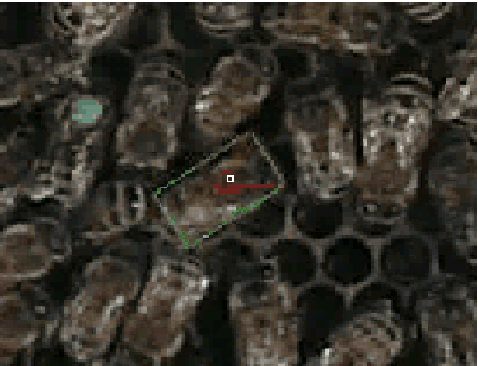
\includegraphics[width=0.23\linewidth]{changepoints/figs/app/tracker-1.png} \hspace{2em}
    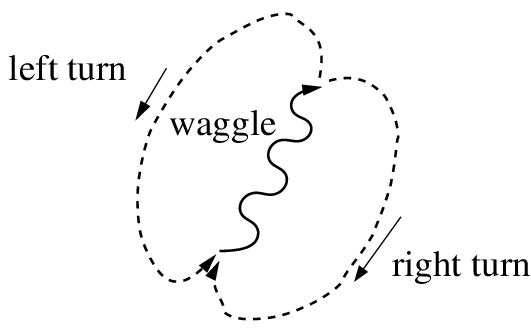
\includegraphics[width=0.27\linewidth]{changepoints/figs/app/bee_dance-1.png}
\caption{Dancer bees are tracked by a appearance based tracker from video sequences. The tracked bee is shown in green rectangle in the left figure above. The right figure shows a stylized bee dance through which bees talk to the other bees about the orientation and distance to the food sources.}
\label{fig:bees}
\end{figure}

\begin{figure}[H]
    \centering
    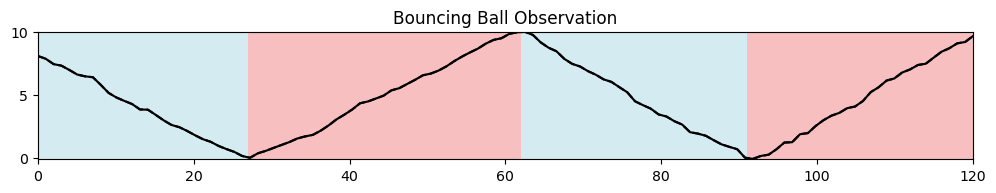
\includegraphics[width=0.85\linewidth]{changepoints/figs/ex/ex0.png}
    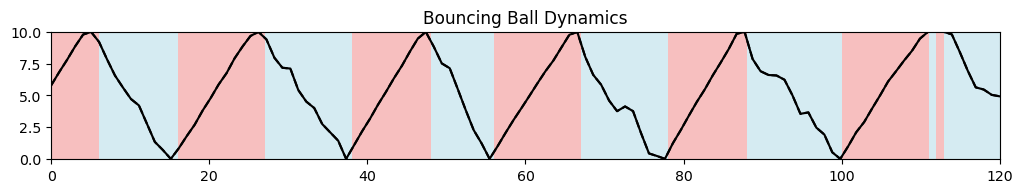
\includegraphics[width=0.85\linewidth]{changepoints/figs/ex/ex1.png}
    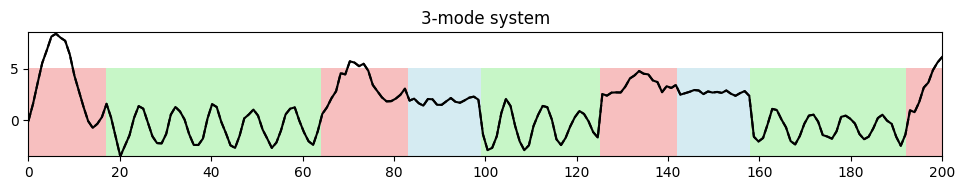
\includegraphics[width=0.85\linewidth]{changepoints/figs/ex/ex2.png}
    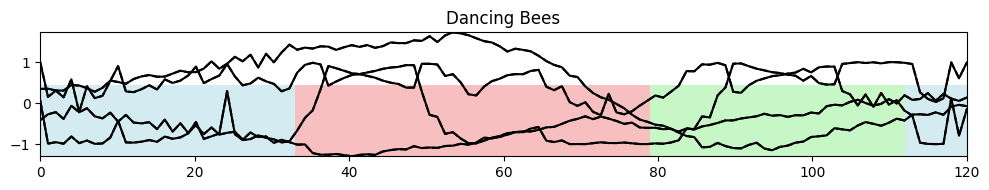
\includegraphics[width=0.85\linewidth]{changepoints/figs/ex/ex3.png}
    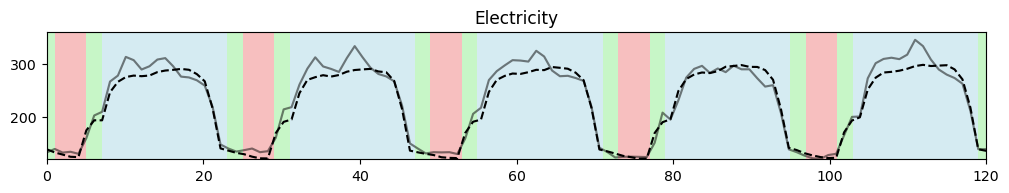
\includegraphics[width=0.85\linewidth]{changepoints/figs/ex/ex4.png}
    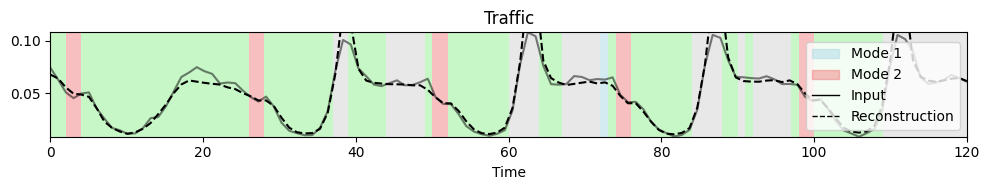
\includegraphics[width=0.85\linewidth]{changepoints/figs/ex/ex5.png}
\caption{Examples of datasets and prediction results. Dotted line represents prediction whereas solid lines represents ground truth; background colors
represent the different operating modes segmented by our base predictor RED-SDS.}
\label{fig:examples}
\end{figure}

\newpage
\subsection{Additional Experiments}
\label{app:more_experiments}

\paragraph{Additional Baselines} We add comparison to three more baselines that handles distribution shift in time series data. They are DtACI \cite{angelopoulos2024online},  ECI \cite{wu2025error}, and L-ARC \cite{zecchin2024localized}.

We would like to emphasize that these baselines are reactive. The question we try to address with CPTC is - what happens when we can anticipate distribution shift? CPTC is designed such that it greatly improves coverage compared to purely reactive methods, while still maintaining the ability to adapt to unknown shifts. To our knowledge, there are no other models that explore the same problem; CPTC provides practitioners with a simple and sound solution, when they have the ability (such as via a state space model) to predict shifts.

\begin{table}[h]
\caption{Performance on synthetic and real-world datasets with target confidence $1-\alpha = 0.9$ (for horizon $T=200$ for synthetic datasets, $300$ for electricity and traffic, and $60$ for bee, mean $\pm$ standard deviation of the test samples).  Methods that are \textit{invalid} (coverage below $90\%$) are grayed out. Our method achieves a high level of calibration (coverage is close to $90\%$) consistently. }
\vspace{1em}
\label{tab:baselines}
\centering
\resizebox{0.8\textwidth}{!}{%
\begin{tabular}{ l | c | c  c c c } 
\toprule
& & DtACI & ECI-cutoff & L-ARC & Ours \\ 
\midrule\midrule
\multirow{2}{*}{\begin{tabular}{l}Bouncing  \\ Ball obs.\end{tabular}} & Cov & \color{gray}{82.97 \plusminus 1.35}& \color{gray}{79.86 \plusminus 1.42}& \color{gray}{75.12 \plusminus 9.25} & 92.06 \plusminus 1.93\\ 
 & Width & \color{gray}{3.21 \plusminus 0.80}& \color{gray}{3.02 \plusminus 0.72}& \color{gray}{1.89 \plusminus 0.76} & 10.70 \plusminus 3.01\\ 
\midrule
\multirow{2}{*}{\begin{tabular}{l}Bouncing  \\ Ball dyn.\end{tabular}} & Cov & \color{gray}{79.63 \plusminus 1.10}& \color{gray}{80.91 \plusminus 1.28}& \color{gray}{78.63 \plusminus 6.21} & 90.62 \plusminus 3.85\\ 
 & Width & \color{gray}{3.51 \plusminus 2.20}& \color{gray}{2.32 \plusminus 0.19}& \color{gray}{2.44 \plusminus 0.23} & 10.73 \plusminus 3.67\\ 
\midrule
\multirow{2}{*}{\begin{tabular}{l}3-Mode \\ System\end{tabular}} & Cov & \color{gray}{88.82 \plusminus 0.95}& \color{gray}{83.67 \plusminus 0.89}& 92.58 \plusminus 2.77 & 90.43 \plusminus 1.92\\ 
 & Width & \color{gray}{12.55 \plusminus 7.52}& \color{gray}{2.39 \plusminus 0.48}& 12.31 \plusminus 2.85 &  4.80 \plusminus 2.64\\ 
\midrule
\midrule
\multirow{2}{*}{\begin{tabular}{l}Traffic\end{tabular}} & Cov & \color{gray}{89.14 \plusminus 0.40}& \color{gray}{86.12 \plusminus 0.50}& 90.05 \plusminus 6.24 & 92.38 \plusminus 1.24\\ 
 & Width & \color{gray}{10.35 \plusminus 9.85}& \color{gray}{7.02 \plusminus 9.72}& 8.39 \plusminus 10.13 & 15.83 \plusminus 5.96\\ 
\midrule
\multirow{2}{*}{\begin{tabular}{l}Electricity\end{tabular}} & Cov & \color{gray}{88.35 \plusminus 0.38}& \color{gray}{89.41 \plusminus 0.47}& \color{gray}{86.42 \plusminus 4.96} & 91.19 \plusminus 1.22\\ 
 & Width & \color{gray}{189.51 \plusminus 187.25}& \color{gray}{138.72 \plusminus 83.30}& \color{gray}{157.82 \plusminus 95.02} & 249.46 \plusminus 1365.46 \\ 
\midrule
\multirow{2}{*}{\begin{tabular}{l}Dancing \\ Bees\end{tabular}} & Cov & \color{gray}{78.91 \plusminus 3.02}& \color{gray}{80.12 \plusminus 2.85}& \color{gray}{75.92 \plusminus 14.21} & 95.71 \plusminus 4.95 \\
 & Width & \color{gray}{0.03 \plusminus 0.01}& \color{gray}{0.08 \plusminus 0.01}& \color{gray}{0.28 \plusminus 0.15} & 0.33 \plusminus 0.14 \\
\bottomrule
\end{tabular}
}
\end{table}

\paragraph{Longer horizon Data} Result for the same set of experiments performed on longer horizon  ($T=10,000$ for synthetic datasets amd $T=4,000$ for Electricity and Traffic datasets) is presented in table \ref{tab:baselines_long_horizon}. We added the setting where the added noise to the bouncing ball dataset is varying over the course of the time series, which is more challenging than the original settings. In the longer horizon case, both SPCI and HopCPT achieve their state of the art performance. Our method remains valid yet achieves less sharp interval width. 

\begin{table}[H]
\caption{Longer time horizon ($T=10,000$ for synthetic datasets amd $T=4,000$ for Electricity and Traffic datasets). Performance in synthetic and real-world datasets with target confidence $1-\alpha = 0.9$. Methods that are \textit{invalid} (coverage below $90\%$) are grayed out. Our method achieves a high level of calibration (coverage is close to $90\%$) consistently.} \vspace{0.5em}
\label{tab:baselines_long_horizon}
\centering
\resizebox{\textwidth}{!}{%
\begin{tabular}{ l | c | c  c c c c c }\toprule
& & RED-SDS & CP & ACI & SPCI  & HopCPT & Ours \\
\midrule\midrule
\multirow{2}{*}{\begin{tabular}{l}Bouncing Ball \\ obs.\end{tabular}} & Cov & \color{gray}{89.31 \plusminus 5.15}& \color{gray}{81.55 \plusminus 7.10} & 89.25 \plusminus 1.40 & 90.05 \plusminus 0.04 & 90.02 \plusminus 0.02 & 90.53 \plusminus 0.23\\
 & Width & \color{gray}{2.65 \plusminus 0.11}& \color{gray}{2.65 \plusminus 0.85}& 3.53 \plusminus 0.81& 1.95 \plusminus 0.12 & 1.99 \plusminus 0.08 & 2.25 \plusminus 0.54\\
\midrule
\multirow{2}{*}{\begin{tabular}{l}Bouncing Ball \\ dyn.\end{tabular}} & Cov & \color{gray}{45.12 \plusminus 25.50}& \color{gray}{42.88 \plusminus 6.95}& \color{gray}{87.95 \plusminus 1.05}& 90.04 \plusminus 0.04 & 90.01 \plusminus 0.04 & 90.05 \plusminus 0.04\\
 & Width & \color{gray}{1.67 \plusminus 0.13}& \color{gray}{0.95 \plusminus 0.51}& \color{gray}{3.10 \plusminus 1.04}& 3.24  \plusminus 0.14 & 3.07 \plusminus 0.10 & 3.18 \plusminus 0.91\\
\midrule
\multirow{2}{*}{\begin{tabular}{l}3-Mode \\ System\end{tabular}} & Cov & \color{gray}{68.52 \plusminus 3.53}& \color{gray}{65.24 \plusminus 5.51}& 89.75 \plusminus 0.90& 90.05 \plusminus 0.02 & 90.02 \plusminus 0.04 & 90.08 \plusminus 0.05\\
 & Width & \color{gray}{2.56 \plusminus 0.21}& \color{gray}{2.33 \plusminus 0.63}& 3.74 \plusminus 0.61& 2.67 \plusminus 0.94 & 2.49 \plusminus 1.31 &  3.12 \plusminus 2.63\\
\midrule
\midrule
\multirow{2}{*}{\begin{tabular}{l}Bouncing Ball \\ obs. varying\end{tabular}} & Cov & \color{gray}{60.83 \plusminus 22.53}& \color{gray}{40.25 \plusminus 6.52}& 88.60 \plusminus 1.25& 90.02 \plusminus 0.04 & 90.04 \plusminus 0.00 & 90.10 \plusminus 0.03\\
 & Width & \color{gray}{2.10 \plusminus 0.45}& \color{gray}{1.73 \plusminus 0.91}& 3.70 \plusminus 0.95 & 2.11 \plusminus 0.82 & 2.14 \plusminus 0.73 & 2.41 \plusminus 1.22\\
\midrule
\multirow{2}{*}{\begin{tabular}{l}Bouncing Ball \\ dyn. varying\end{tabular}} & Cov & \color{gray}{44.25 \plusminus 26.11}& \color{gray}{41.73 \plusminus 7.12}& \color{gray}{88.05 \plusminus 1.00}& 90.05 \plusminus 0.03 & 90.02 \plusminus 0.04 & 90.08 \plusminus 0.03\\
 & Width & \color{gray}{1.85 \plusminus 0.12}& \color{gray}{0.92 \plusminus 0.55}& \color{gray}{3.13 \plusminus 1.14}& 2.92 \plusminus 0.21 & 3.05 \plusminus 0.19 & 3.40 \plusminus 0.32\\
\midrule
\midrule
\multirow{2}{*}{\begin{tabular}{l}Traffic\end{tabular}} & Cov & \color{gray}{87.14 \plusminus 10.51}& \color{gray}{70.52 \plusminus 2.83}& \color{gray}{89.15 \plusminus 0.38}& 90.01 \plusminus 0.04 & 90.03 \plusminus 0.03 & 90.02 \plusminus 0.03\\
 & Width & \color{gray}{2.91 \plusminus 1.62}& \color{gray}{0.43 \plusminus 0.25}& \color{gray}{55.10 \plusminus 24.13}& 4.81 \plusminus 2.42 & 7.84 \plusminus 10.53 & 8.55 \plusminus 14.11\\
\midrule
\multirow{2}{*}{\begin{tabular}{l}Electricity\end{tabular}} & Cov & \color{gray}{76.10 \plusminus 13.52}& \color{gray}{69.53 \plusminus 3.21}& \color{gray}{89.05 \plusminus 0.33}& 90.02 \plusminus 0.03 & 90.00 \plusminus 0.02 & 90.43 \plusminus 0.03\\
 & Width & \color{gray}{91.30 \plusminus 125.10}& \color{gray}{62.10 \plusminus 451.20}& \color{gray}{31.40 \plusminus 171.30}& 162.02 \plusminus 11.40 & 161.70 \plusminus 15.20 & 173.38 \plusminus 31.10 \\
\bottomrule
\end{tabular}
}
\end{table}

\paragraph{Aggregation methods.} In this study we compare the two different aggregation methods. First is the case where we chose the minimum size, i.e. $\Gamma_t(x_t) = $ \Eqref{eq:aggregation-average}. Algorithmically, we discretize the output space $\mathcal{Y}$ into intervals of length 0.02, and calculate probability mass for each interval. We refer to this method as \emph{min}. Aggregation by union numbers (the same as in the main text using \Eqref{eq:aggregation-union}) are referred to as \emph{union}. Results are present in table \ref{tab:aggregation} where the performance are very similar. When there are two modes (bouncing ball cases) the prediction intervals are almost identical.
 
\begin{table}[h!]
\centering
\caption{Ablation Study on two different Union (\textit{union}, \eqref{eq:aggregation-union}) and grid-discretization (\textit{min}, \eqref{eq:aggregation-average}).}
\vspace{0.5em}
\label{tab:aggregation}
\begin{tabular}{lcccccc}
\toprule
& BB obs. & BB dyn. & 3-mode system & traffic & electricity & bees \\
\midrule
\midrule
Coverage (\textit{union}) & 90.53 & 90.44 & 93.35 & 92.76 & 92.62 & 93.43 \\
Coverage (\emph{min})  & 90.03 & 90.32 & 91.50 & 91.87 & 89.82 & 90.28 \\
Width (\textit{union})   & 3.73  & 1.72  & 2.45 & 7.94  & 166.88 & 0.79 \\
Width (\emph{min})     & 3.62 & 1.65  & 2.41 & 7.95  & 153.57 & 0.77 \\
\bottomrule
\end{tabular}
\end{table}

\paragraph{Discussion on Misspecified Regimes.} We designed the number of latent states to be a hyperparameter given by the user. Our method ensures that the validity guarantee still holds even if the state cardinality is incorrect (theorem 4.2), as incorrect state cardinality can be formulated as a case of incorrect classification. Determining state space cardinality is a well-studied problem (see for example \cite{branicky1994stability}), and we consider it to be beyond the scope of our paper.

Regarding the effect on performance, our ablation studies (Section 5.2, Tables \ref{tab:z_exp} and \ref{tab:z_exp_area}) demonstrate that while the validity (coverage) of CPTC is robust to errors in state prediction, the sharpness (width of prediction intervals) can be affected. Table 3 explicitly shows that "the more accurate the state prediction is, the sharper the intervals." This implies that selecting a more appropriate number of regimes that better captures the true underlying dynamics would lead to narrower and more efficient prediction intervals.

\subsection{Qualitative Results}
\label{app:pictures}

We provide additional visualizations to present qualitative comparisons of CPTC compared to baseline models. Figures \ref{fig:synthetic}, \ref{fig:pic2}, and \ref{fig:pic3} show consistent results with the analysis in section 5, where CPTC shows stronger adaptivity and validity for uncertainty quantification in time series with these nonstationary dynamics.



\begin{figure}[h!]
    \centering
    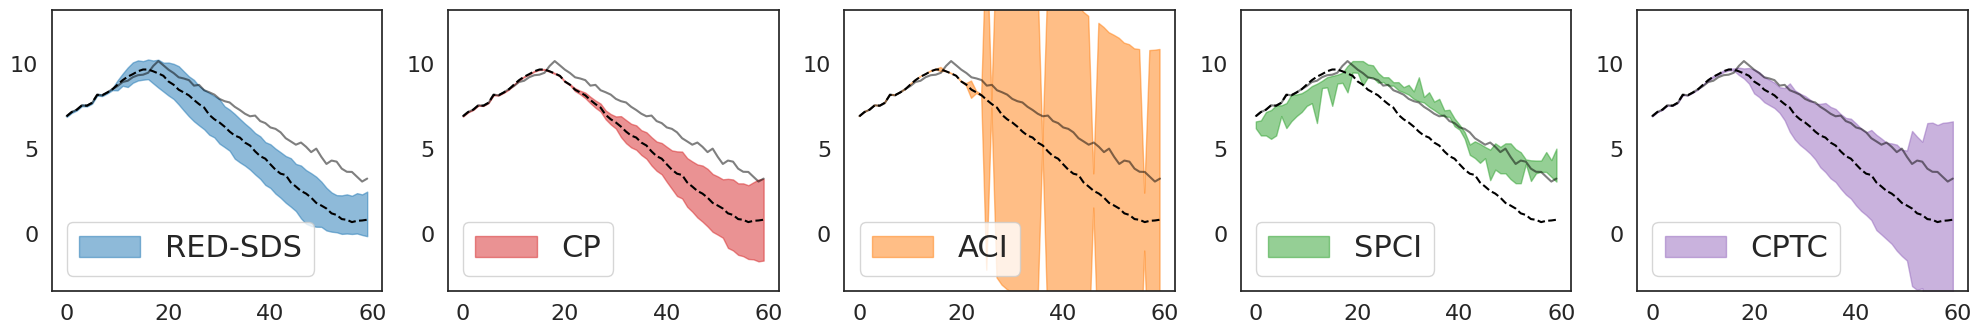
\includegraphics[width=\linewidth]{changepoints/figs/ex/a.png}
    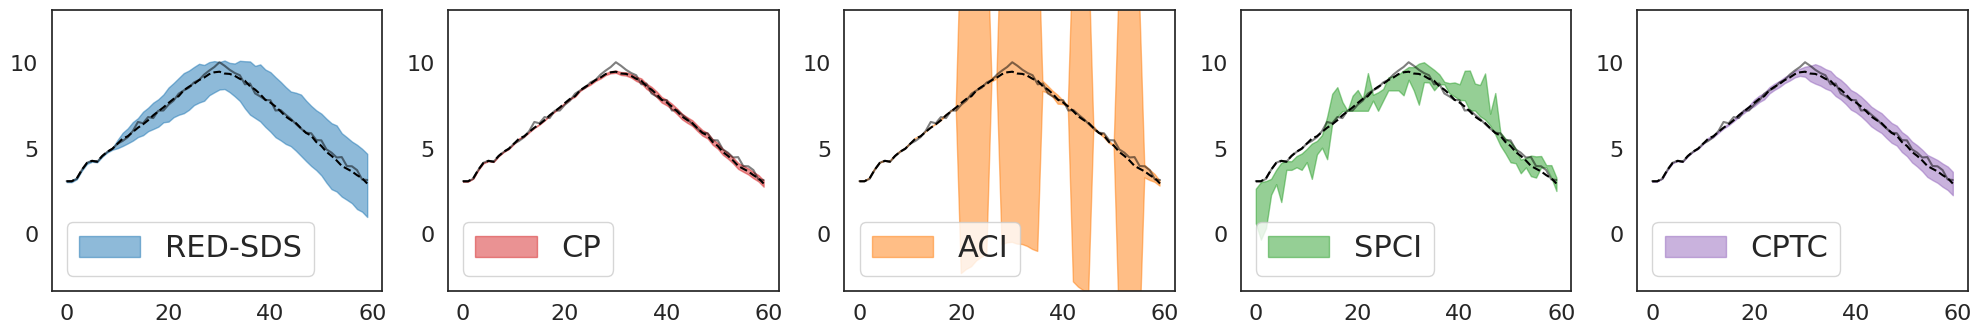
\includegraphics[width=\linewidth]{changepoints/figs/ex/b.png}
    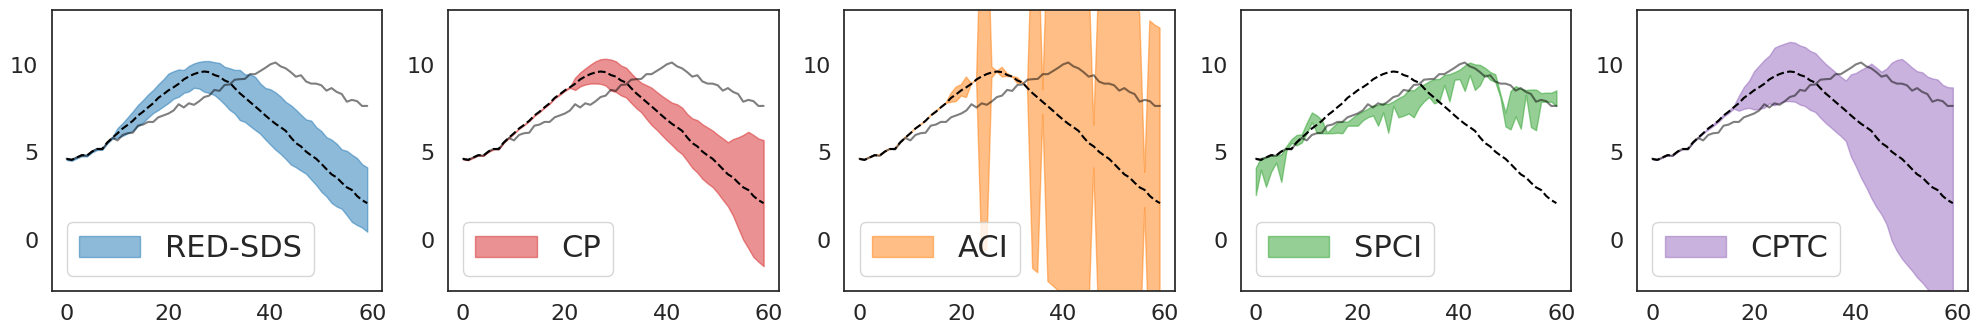
\includegraphics[width=\linewidth]{changepoints/figs/ex/c.png}
    \caption{\textbf{Qualitative comparison of the prediction interval on the bouncing ball w/ dynamics noise dataset.} The dashed line is the predicted state whereas the solid gray line is the observation. We see that our CPTC algorithm can increase the interval in anticipation of an uncertain state change (top panel), is stabler when the prediction is accuracy compared to ACI and SPCI (middle panel), and is adaptive to inaccurate predictions (botom panel).}
    \label{fig:synthetic}
     %\vspace{-0.5em}
\end{figure}


% \begin{figure}[H]
%     \centering
%     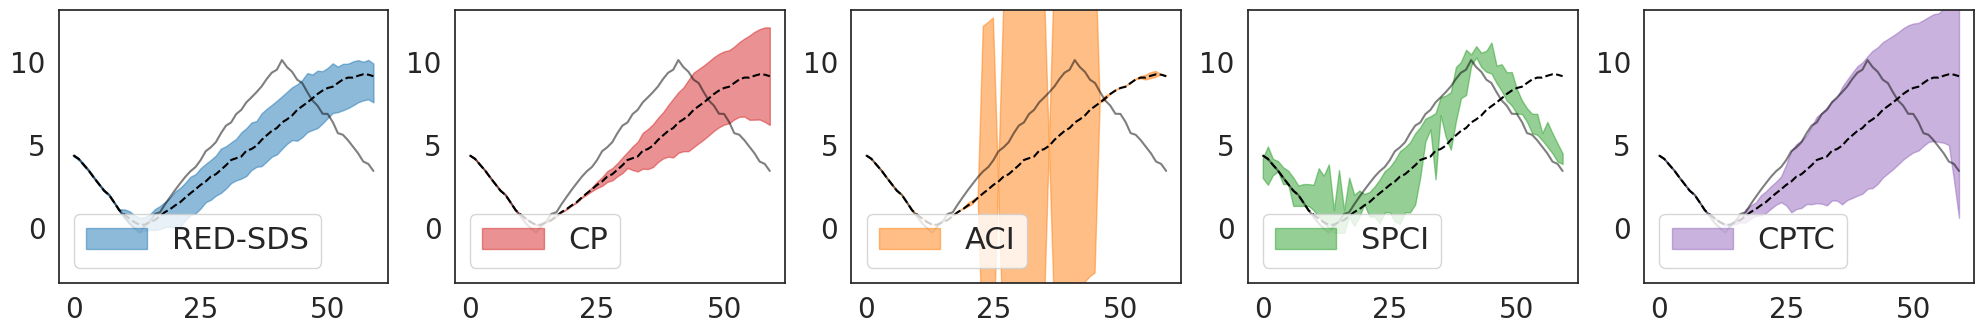
\includegraphics[width=\linewidth]{changepoints/figs/app/a1.png}
%     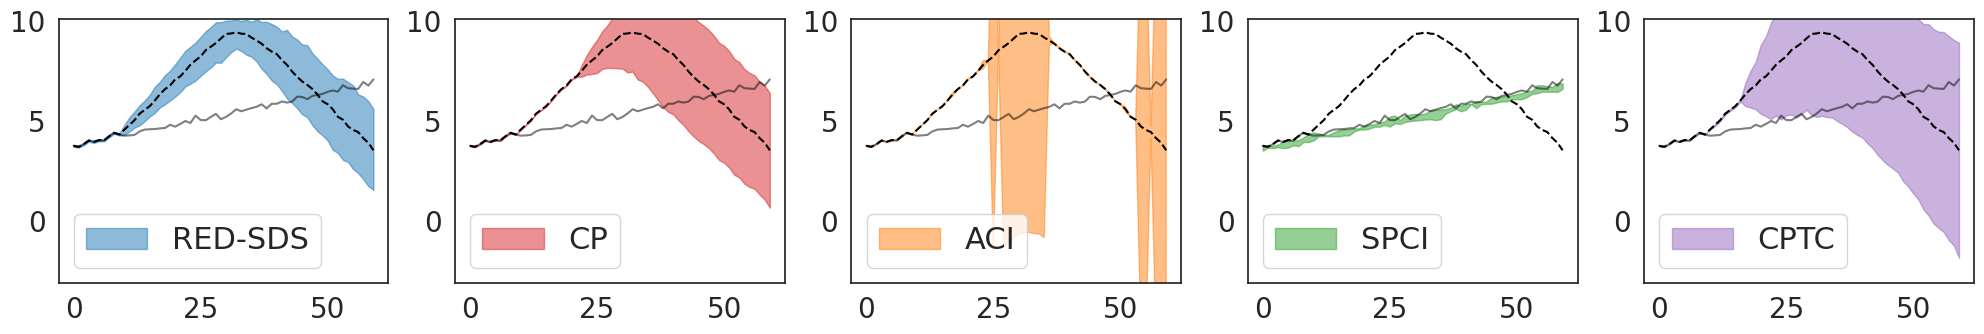
\includegraphics[width=\linewidth]{changepoints/figs/app/a2.png}
%     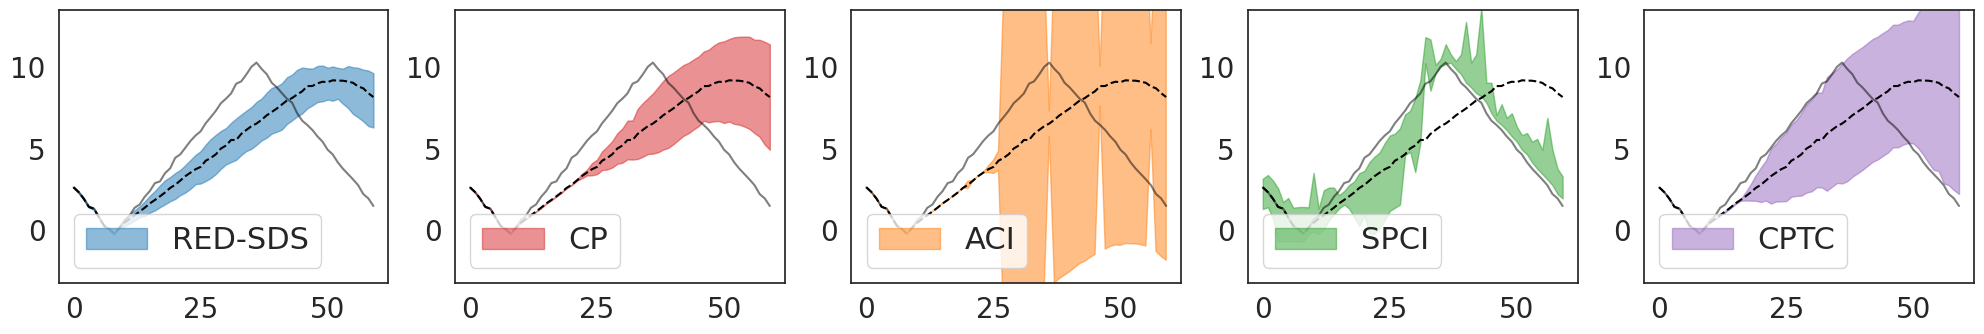
\includegraphics[width=\linewidth]{changepoints/figs/app/a3.png}
%     \caption{Visualization of prediction intervals on the Bouncing Ball Obs dataset.}
%     \label{fig:pic1}
%     \vspace{-1em}
% \end{figure}
\vspace{-1em}
\begin{figure}[H]
    \centering
    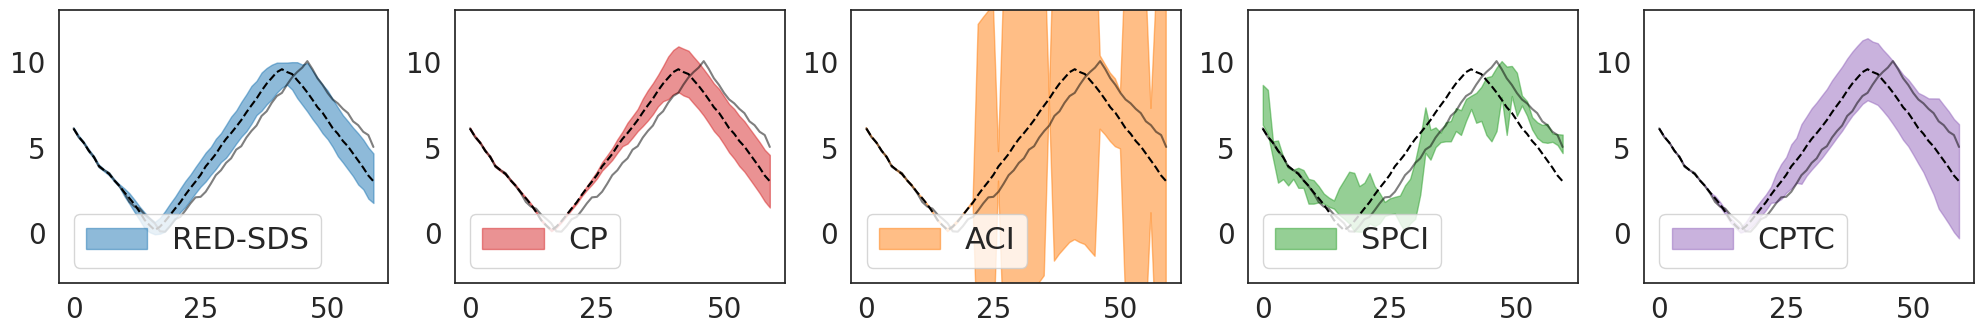
\includegraphics[width=\linewidth]{changepoints/figs/app/b1.png}
    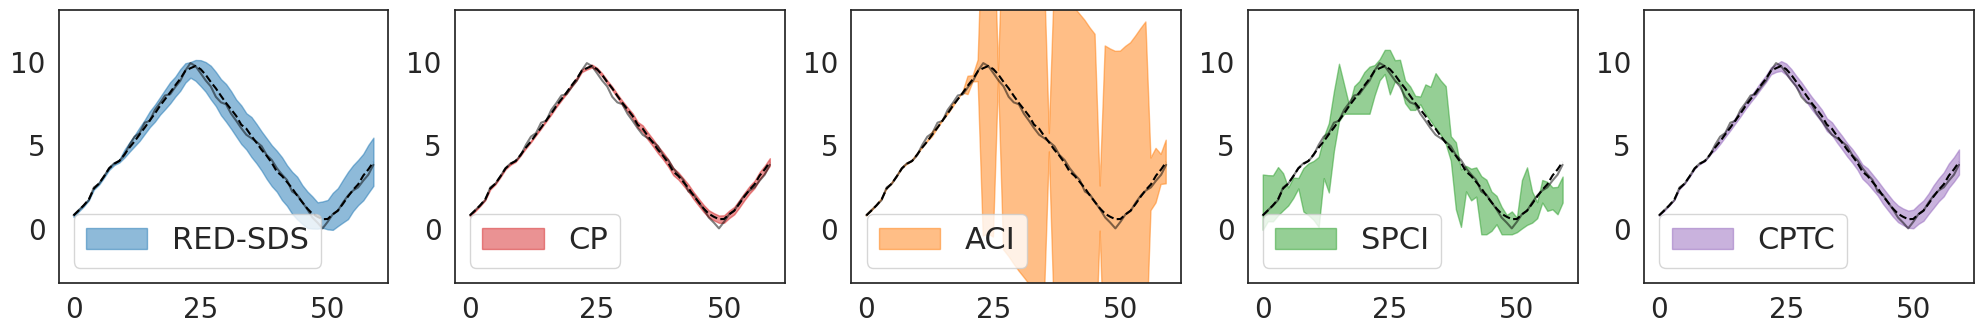
\includegraphics[width=\linewidth]{changepoints/figs/app/b2.png}
    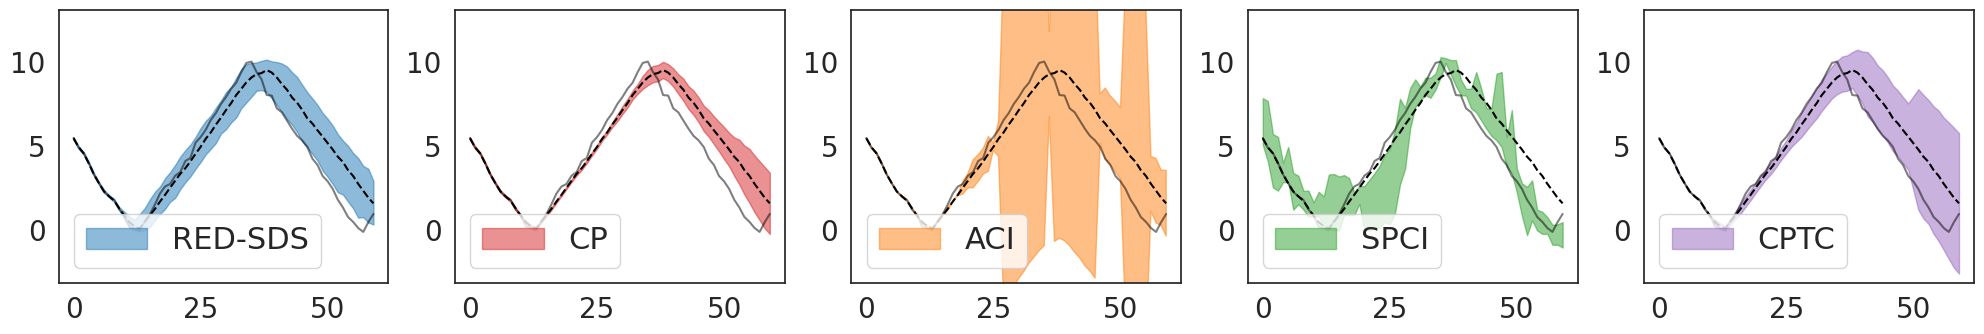
\includegraphics[width=\linewidth]{changepoints/figs/app/b3.png}
    \caption{Visualization of prediction intervals on the Bouncing Ball Obs dataset.}
    \label{fig:pic2}
\end{figure}
\vspace{2em}

\begin{figure}[H]
    \centering
    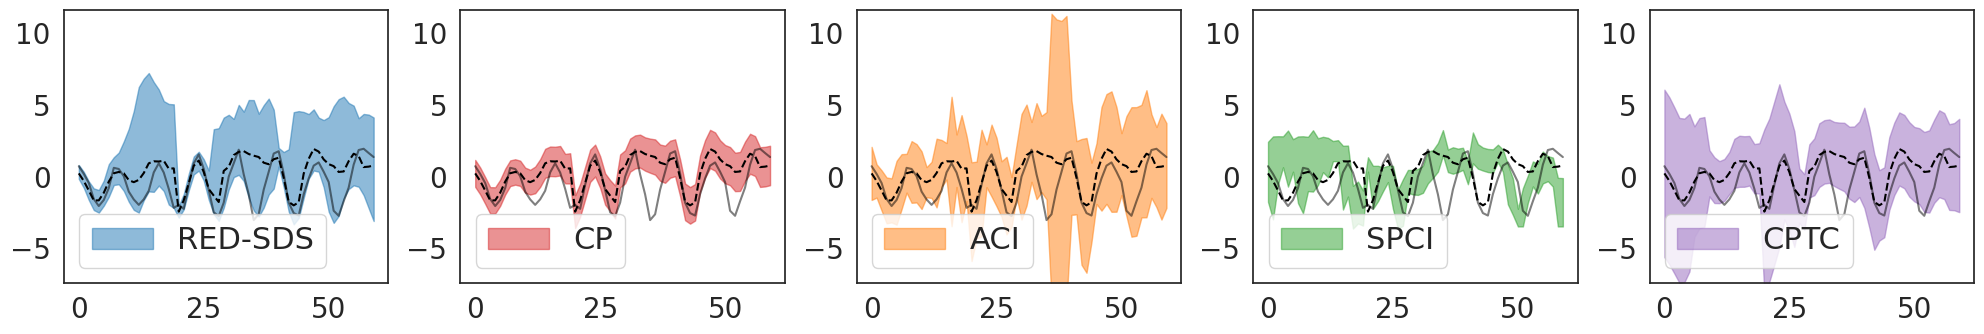
\includegraphics[width=\linewidth]{changepoints/figs/app/c1.png}
    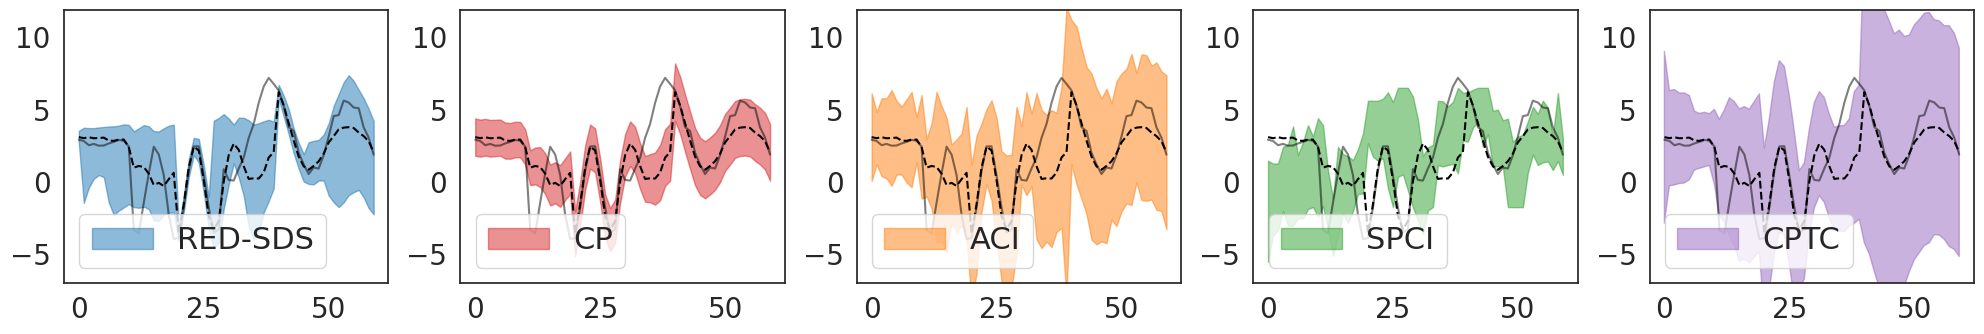
\includegraphics[width=\linewidth]{changepoints/figs/app/c2.png}
    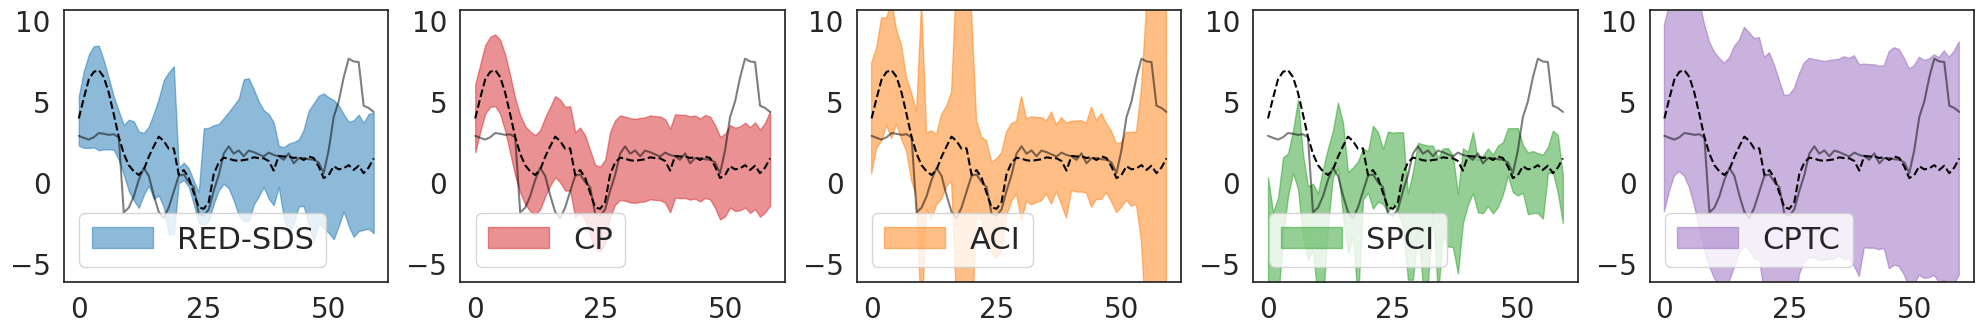
\includegraphics[width=\linewidth]{changepoints/figs/app/c3.png}
    \caption{Visualization of prediction intervals on the 3 mode system datasets.}
    \label{fig:pic3}
\end{figure}

\section{Runtime analysis}

We provide a runtime analysis comparing the aggregation methods in Equations \ref{eq:aggregation-average} and \ref{eq:aggregation-union} and with baselines.

\textbf{Notation}

\begin{itemize}
    \item $T$: Total timesteps, $K$: Number of states, $M$: State prediction model inference complexity
    \item Score sets $\mathcal{S}_z$ maintained in sorted order (quantile computation in $\mathcal{O}(1)$, insertion $\mathcal{O}(\log T)$)
\end{itemize}

\textbf{Complexity Per Timestep}

\begin{enumerate}
    \item Computing quantile $Q^{1-\alpha_t}(\mathcal{S}_z^{(l)})$ for each state, totaling $\mathcal{O}(K)$.
    \item State Prediction: computing $\hat{p}(z_t|x_t)$ and sampling a state, totaling $\mathcal{O}(M)$.
    \item Aggregation
    \begin{itemize}
        \item \textit{Eq. 10, Weighted Level-Set:} $\mathcal{O}(K \cdot \lceil 1/\delta \rceil^d)$ where $\delta$ is discretization resolution
        \item \textit{Eq. 11, Union:} $\mathcal{O}(K \log K)$ for sorting states by probability
    \end{itemize}
    \item Updates: $\mathcal{O}(\log t)$ for inserting new score into sorted set.
\end{enumerate}

\textit{Therefore, the total complexity of CPTC with horizon $T$ is:}

$\mathcal{O}(T \cdot (M + K \cdot \lceil \frac{1}{\delta} \rceil^d) + T \log T)$ if we use the Weighted Level-Set as aggregation in Eq. 10, and

$\mathcal{O}(T \cdot (M + K \log K) + T \log T)$ if we use the more efficient Union aggregation in Eq. 11.

In practice, both $M$ (inference cost) and $K$ (number of discrete states) are small. For applications where $K = \mathcal{O}(1)$ and $M = \mathcal{O}(1)$, CPTC achieves near-linear scaling $\mathcal{O}(T \log T)$, the same as ACI (see table below).

If we use the more precise weighted level set aggregation method, the runtime largely depends on the discretization resolution $\delta$, output dimension $d$, and the number of states $K$. We remark the level set approach scales poorly if the resolution, dimension, or number of states are high.

\begin{table}[h]
\centering
\begin{tabular}{lll}
\hline
\textbf{Method} & \textbf{Time Complexity} & \textbf{Remarks} \\
\hline
ACI & $\mathcal{O}(T \log T)$ & Single score set, no state awareness \\
SPCI / HopCPT & $\mathcal{O}(T^2 \log T)$ & Re-train regression model at every time step \\
CPTC (Union) & $\mathcal{O}(T \log T)$ & State-aware, pre-trained predictor \\
\hline
\end{tabular}
\end{table}
% \subsection{Ablation study on non state-dependent forecaster}

% We can still use CPTC when we only have one forecaster but have access to some state prediction (for example in the form of external parameters). We can apply algorithm \ref{alg:cptc} directly with the special case where $\hat{f}(x,z_i) = \hat{f}(x,z_j)$ for any $x \in \gX and z_i, z_j \in \gZ$. Table \ref{tab:one_forecaster} presents the performance of the algorithm in this case.

% \begin{table}[]
% \caption{One forecaster} %\vspace{-0.5em}
% \label{tab:one_forecaster}
% \centering
% \begin{tabular}{ l | c | c  c } 
% \toprule
% & & SPCI  & Ours \\
% \midrule\midrule
% \multirow{2}{*}{\begin{tabular}{l}Bouncing Ball \\ obs.\end{tabular}} & Cov & \color{gray}{37.90 \plusminus 9.78} & 92.16 \plusminus 26.88\\ 
%  & Width & \color{gray}{1.45 \plusminus 0.85} & 7.43 \plusminus 4.68\\ 
% \midrule
% \multirow{2}{*}{\begin{tabular}{l}Bouncing Ball \\ dyn.\end{tabular}} & Cov & \color{gray}{53.62 \plusminus 7.75} & 90.58 \plusminus 29.21\\ 
%  & Width & \color{gray}{2.02 \plusminus 0.23} & 8.11 \plusminus 4.93\\ 
% \midrule
% \multirow{2}{*}{\begin{tabular}{l}3-Mode \\ System\end{tabular}} & Cov & \color{gray}{81.72 \plusminus 2.88} & 93.35 \plusminus 3.51\\ 
%  & Width & \color{gray}{3.94 \plusminus 0.85} & 13.68 \plusminus 2.49\\ 
% \midrule\midrule
% \multirow{2}{*}{\begin{tabular}{l}Traffic\end{tabular}} & Cov & \color{gray}{88.24 \plusminus 2.13} & 94.76 \plusminus 4.93\\ 
%  & Width & \color{gray}{4.62 \plusminus 2.28} & 8.34 \plusminus 14.44\\ 
% \midrule
% \multirow{2}{*}{\begin{tabular}{l}Electricity\end{tabular}} & Cov & \color{gray}{86.62 \plusminus 2.97} & 93.82 \plusminus 4.22\\ 
%  & Width & \color{gray}{371.69 \plusminus 305.86} & 98.87 \plusminus 49.35\\ 
% \midrule
% \multirow{2}{*}{\begin{tabular}{l}Dancing Bees\end{tabular}} & Cov & \color{gray}{79.2 \plusminus 0.3} & 93.43 \plusminus 11.42 \\
%  & Width & \color{gray}{1.77 \plusminus 1.38} & 1.15 \plusminus 0.56 \\
% \bottomrule
% \end{tabular}
% \end{table}



% \subsection{Experiment on state prediction (continued) }
% \label{app:z_exp}

% \begin{table*}[h!]
%     \centering
%     \begin{tabular}{c|c c c c}
%         \hline
%         \toprule
%         $T=250$& Ground truth state labels & GT w/ $20\%$ error & GT w/ $50\%$ error & Learned state labels \\ 
%         \midrule
%         BB obs. noise & 90.00 \plusminus 0.32 & 89.94 \plusminus 0.29 & 89.92 \plusminus 0.28 & 89.11 \plusminus 3.54 \\ 
%         BB dyn. noise & 90.04 \plusminus 0.34 & 90.01 \plusminus 0.35 & 89.96 \plusminus 0.30 & 90.11 \plusminus 0.33\\ 
%         3-mode system & 89.34 \plusminus 0.87 &  89.40 \plusminus 0.91  & 89.64 \plusminus 0.80 & 89.72 \plusminus 1.51 \\ 
%         \midrule\midrule
%         $T=1000$& Ground truth state labels & GT w/ $20\%$ error & GT w/ $50\%$ error & Learned state labels \\ 
%         \midrule
%         BB obs. noise & 90.00 \plusminus 0.32 & 89.94 \plusminus 0.29 & 89.92 \plusminus 0.28 & 89.11 \plusminus 3.54 \\ 
%         BB dyn. noise & 90.04 \plusminus 0.34 & 90.01 \plusminus 0.35 & 89.96 \plusminus 0.30 & 90.11 \plusminus 0.33\\ 
%         3-mode system & 89.34 \plusminus 0.87 &  89.40 \plusminus 0.91  & 89.64 \plusminus 0.80 & 89.72 \plusminus 1.51 \\ 
%         \bottomrule
%     \end{tabular}
%     \caption{Coverage of CPTC for using ground truth (GT) labels, GT labels with injected noise, and learned  label predictions on synthetic data with $T=250, 1000$. We can see that coverage performance does not change significantly with error in state prediction. }
%     \label{tab:z_exp_small}
% \end{table*}

% \input{secs/checklist}
% \end{document}



\part{Time series UQ for decision making: applications}
\chapter{Online adaptive anomaly thresholding with confidence sequences}

% \begin{abstract}
% Selecting appropriate thresholds for anomaly detection in online, unsupervised settings is a challenging task, especially in the presence of data distribution shifts. Addressing these challenges is critical in many practical large scale systems, such as infrastructure monitoring and network intrusion detection.
% %
% This paper proposes an algorithm that connects online thresholding with constructing confidence sequences achieving (1) adaptive online threshold selection robust to distribution shifts, (2) statistical guarantees on false positive and false negative rates without any distributional assumptions, and (3) improved performance when given relevant offline data to warm-start the online algorithm, while having bounded degradation if the offline data is irrelevant. We complement our theoretical results with empirical evidence that our method outperforms commonly used baselines across synthetic and real world datasets.
% \end{abstract}

% Choosing a threshold on anomaly scores to classify if a given data point is an anomaly is an important problem. This challenge is exacerbated in the online setting when the anomaly detector is unsupervised and the data-stream undergoes distribution shift. Both of these are common in many practical large scale systems, including those for detecting performance anomalies in computer systems, infrastructure monitoring and network intrusion detection.
% In this paper, we connect the online thresholding problem to that of constructing online confidence sequences. By on this connection, we present an algorithm that can select anomaly thresholds automatically, with guarantees on false positive and false negative rates without making any distributional assumptions. Furthermore, we prove that our algorithm is adaptive to distribution shifts, and can leverage offline data to further improve its performance.
% Ours is the first algorithm for online anomaly thresholding with rigorous statistical guarantees. We complement our theoretical results by showing empirically that our method outperforms commonly used heuristics across a variety of academic and real world datasets.


\section{Introduction and Motivation} 
Online anomaly detection (OAD) is the task of identifying deviations from the normal behavior in a streaming fashion, where samples arrive sequentially, and decisions must be made before the next sample is received. This task plays a fundamental role in various practical applications within cyber and cyber-physical systems, including maintenance \cite{khan2020industrial}, monitoring \cite{hill2010anomaly}, and security \cite{mirsky2018kitsune, lazarevic2003comparative}. In modern environments, the sheer volume and velocity of data make it often impractical to have comprehensive labels for all anomalous samples \cite{siffer2017anomaly, schmidl2022anomaly, ren2019time, audibert2020usad}.

In deployment, typical AD algorithms assign a real-valued anomaly score to each sample, where a higher score indicates a greater degree of anomaly \cite{chandola2009anomaly}. The OAD algorithm first scores each sample and then calibrates a threshold to make the binary decision of whether the given sample is anomalous or not. The choice of this threshold is critical due to its significant downstream impact. In security systems, for example, failing to detect a genuine anomaly or security event can have catastrophic consequences \cite{203674}. Conversely, false positives incur costs, as each detection necessitates investigation by a security operator, potentially leading to `alert fatigue' \cite{202751, lin2018collaborative, he2023cloudshield}.

Given the risk of incorrect decisions, a common methodology to set the threshold is by \emph{abstaining} from decisions for an initial `cold-start' number of samples on the  stream \cite{10.14778/2850583.2850593, katz2023cold}. At the end of the cold-start period, a threshold is chosen for future decision making, either by algorithm or by an expert based on the online scores during the cold-start, as well as any offline data that is available \cite{ren2019time, bhatia2021mstream,huang2022semi, li2021fluxev}. 
This approach has two drawbacks. 
Firstly, using a fixed cold-start duration across all streams independent of stream statistics is sub-optimal and can lead to much more abstains than necessary. Secondly, a static threshold is prone to performance loss when the data stream undergoes distribution shift - a common occurrence in many AD systems \cite{279982,gama2014survey}. Although adapting anomaly scoring to distribution drifts have been studied \cite{ma2018robust,bhatia2022memstream, sankararaman2022fitness}, limited advances have occurred in adapting the threshold dynamically.
%We frame the threshold selection as online quantile estimation and provide guarantees on number of false positives and false negatives that hold even under distribution shifts and provably improve in the presence of offline data. 
%
%scores gathered thus far  (cf. Fig \ref{fig:static_cold_start}). If appropriate, offline data is used along side the online scores during cold-start to minimize risks of incorrect decisions \cite{ren2019time, bhatia2021mstream,huang2022semi, li2021fluxev}. 


%\subsection{Threshold selection as quantile estimation}

We formulate adaptive threshold selection as online quantile estimation by defining anomalies as tail quantile of anomaly scores \cite{steinwart2005classification, cadre2013estimation, gan2017scalable, siffer2017anomaly}. Formally, we model that each time $t \in \mathbb{N}$, the anomaly score $S_t \in \mathbb{R}$ is independently sampled from distribution $f_t$. This score $S_t$ is an {anomaly} if it exceeds the $p$th quantile of the distribution $f_t$. We assume the quantile level $p \in (0,1)$ is known, while the distribution $f_t$ as unknown to the algorithm. 
Knowledge of $p$ arises either from a constraint on the rate of anomalies that can be investigated without succumbing to alert fatigue \cite{hassan2019nodoze, ho2021hopper}, or from domain knowledge \cite{perini2023unsupervised}. 

Performance of threshold selection is measured by false positives (FP), benign samples marked as anomalous, false negatives (FN), anomalous sample mark as benign, and number of samples abstained from making a decision on. Since AD outputs are typically used to make consequential decisions, e.g. engaging human operators to triage alerts, OAD systems must achieve low number of FPs and FNs, by possibly trading-off with abstains \cite{ho2017detecting}. Further, these systems need to be adaptive to distribution shifts and be designed without requiring distributional assumptions (cf. \emph{Research challenges} $5$-$7$ of \cite{sadik2014research}).

 \subsection{Desiderata of OAD threshold selection systems}
 \label{sec:desiderata}

% AD Threshold systems marks each sample as either anomalous, non-anomalous or abstains from decision making \cite{chandola2009anomaly}. Performance is measured by false positives (FP), benign samples marked as anomalous, and false negatives (FN), anomalous sample mark as benign, in addition to number of samples abstained on. Typically, since AD outputs are used to make consequential decisions, e.g. engaging human operators to triage alerts, OAD systems must have low number of FPs and FNs achieved at the cost of abstains \cite{ho2017detecting}. Further, these systems need to be adaptive to distribution shifts and be designed without requiring distributional assumptions (cf. \emph{Research challenges} $5$-$7$ of \cite{sadik2014research} and references therein). In summary, the following set of statistical requirements are desired.

 %the following set of statistical requirements desired for online threshold selection. \cite{sadik2014research}.
 
In summary, the following set of statistical requirements is desired for online threshold selection.
 
    \emph{\textbf{(i) High accuracy:}} Constant number of mistakes\footnote{Throughout, we denote the mistakes as sum of FP and FN.} independent of the stream length on an i.i.d. data-stream.

      \vspace{-1mm}
     \emph{\textbf{(ii) Low abstention:}} Abstain on a vanishing fraction of samples on an i.i.d. stream, i.e. small cold-start period. 

     \vspace{-1mm}
    \emph{\textbf{(iii) Adaptive to distribution changes:}} On a non-stationary stream, number of mistakes and abstains only increase compared to the stationary setting by a constant factor that is independent of the stream length, but only proportional to the number and magnitude of distribution changes. 
    
    \vspace{-1mm}
       \emph{\textbf{(iv) Learn from offline dataset:}} When unlabeled offline datasets are available, abstain rate is a constant independent of stream length, as long as the online distribution matches one of the offline distribution. In the worst-case of arbitrary offline dataset distribution, performance degradation compared to no offline dataset must be bounded independent of stream length and size of the dataset.

       \vspace{-1mm}

       \emph{\textbf{(v) Distribution and parameter free:}} The algorithm does not require any knowledge of the distributions or assumptions such as sub-gaussian tails or parameterized distribution family, and nevertheless must guarantee all of above.
     %The algorithm however does not know apriori if the online stream and offline dataset are from the same distribution.
% \begin{enumerate}[itemsep=0pt,topsep=-2pt, labelindent=-1pt,labelwidth=!]
%     \item \textbf{High accuracy:} Constant, independent of the stream length, number of mistakes\footnote{Throughout, we denote the mistakes as sum of FP and FN.}, on an i.i.d. data-stream.
%     \item \textbf{Low abstention:} Abstain on a vanishing fraction of samples on an i.i.d. stream, i.e., small cold-start period. 
%     \item \textbf{Adaptive to distribution shifts:} On a non-stationary stream, the FPs, FNs and abstains only increase compared to the stationary setting by a constant factor that is independent of the stream length, but only proportional to the number and magnitude of distribution changes. The algorithm however cannot know apriori the number of changes on the stream.
%     \item \textbf{{\color{black} Learn from offline data:}} If there is access to multiple unlabeled offline datasets, then the fraction of abstains is a constant independent of stream length, whenever the online distribution matches one of the offline distribution. However, if none of the offline distributions matches the online stream, the performance must be comparable to the setting without offline data. %The algorithm however does not know apriori if the online stream and offline dataset are from the same distribution.
%     \item \textbf{Distribution and parameter free:} The algorithm does not require any knowledge of the distributions or assumptions such as sub-gaussian tails or the distribution family being parameterized, nevertheless must guarantee all of the aforementioned performance.
% \end{enumerate}

%Crucially, we want the above desiderata to be satisfied without any assumptions on the distribution such as tails or parametric form. 




%The online version of the unsupervised AD problem is one where samples are presented to the AD algorithm one at a time in a streaming fashion. At each time step, the AD algorithm outputs an anomaly score based on the samples seen thus far. As the problem is unsupervised, the ground-truth label of the sample is not available to the AD algorithm before making its next set of predictions. This unsupervised, OAD is a common abstraction for many problems in cloud-computing, performance monitoring and network intrusion detection systems .

%Typical performance measures of anomaly detection algorithms are AUC (Area under the curve) of the ROC (Receiver operating curve). This measure is computed by comparing the anomaly scores output by the AD algorithm and the ground-truth binary labels by sweeping over all possible choice of anomaly thresholds. However, 

% \paragraph{Anomaly thresholding.}  Most modern AD algorithms outputs an anomaly score for a given sample and are evaluated using threshold-agnostic metrics such as AUCROC. The choice of how to choose a threshold is often left unstudied and unreported. This is especially surprising since in practice, tuning thresholds is an important problem and critical to the performance of any AD system \cite{chandola2009anomaly, hundman2018detecting} 


\subsection{Main result and technical contributions}

{Algorithm \ref{alg:five} is distribution and parameter free and is the \emph{first algorithm to satisfy all the aforementioned desiderata.}}  Algorithm \ref{alg:five} does not require knowledge on the locations or number of distribution shifts nor on the online stream or the offline datasets' distributions. Nevertheless, under mild technical assumptions, the guarantees in Theorem \ref{thm:core_theorem} show that the performance adapts to the problem complexity.
%, if any stationary segment of the online stream matches any of the offline datasets' distirbution, the number of abstains and mistakes are small. On the other hand if a stationary segment in the online distribution is arbitrary and does not match any offline datasets' distribution, then the performance on this segment is comparable to one in which no offline data is present.
%However, the algorithm does not need as input any prior information, but rather its performance adapts to the complexity of the online data stream. 
%In particular, FP, FN and abstain are lower when there is fewer distribution shifts and/or offline datasets have the same distribution as the online stream, with the bounds naturally identifying the problem complexity parameter. 
%\subsection{Technical Contributions}
Concretely, our contributions are as follows.

{\color{black} \textbf{1. High accuracy requires abstention.} We prove that any  scheme that does not abstain,  cannot achieve constant FPs and FNs, even for a stationary stream. The proof follows by constructing a hard instance and a reduction from decision making to hypothesis testing on that instance. }

{\color{black} \textbf{2. Algorithm using confidence sequences (CS) to adapt threshold to distribution changes.} 
%  Threshold using confidence sequence (CS) to be adaptive to changes in distribution.
%We connect OAD and threshold selection with confidence sequences (CS). 
%We use  CS to make decisions to yield high-accuracy and a data-dependent abstain. 
A sample $S_t$ is deemed as an anomaly by our algorithm (Algo. \ref{alg:five}) if it exceeds the upper confidence of the $p$th quantile,  is benign if it is smaller than the lower confidence, and is abstained from otherwise (Fig. \ref{fig:motivation_alg_1}). The crux of our algorithm is in choosing the \emph{relevant online and offline samples} to construct the CS. Online distribution shifts are detected by constructing CS on different sub-sequences and testing if they have a non-empty intersection. Theorem \ref{the:iid} shows that on an i.i.d. stream of length $T$, no mistakes  and at-most $\mathcal{O}(\sqrt{T})$ abstains occur with high probability. 
%3. \textbf{Confidence sequences can provably be adaptive to distribution shifts.} 
Theorem \ref{thm:online_shift} shows that when there are distribution shifts, our algorithm incur total additional mistakes \emph{independent} of $T$, without requiring any knowledge of the data distributions or change-points.
%our algorithm, without requiring any knowledge of the distributions or change-points, incurs an additional factor \emph{independent} of $T$ mistakes and abstains compared to the stationary stream.

% The CS for the $p$th quantile is a sequence of random intervals $([l_t, u_t])_{t \geq 1}$ such that for all $t \geq 1$, {\em(i)} $l_t \leq u_t$ almost-surely are measurable functions of $S_1, \cdots, S_t$, and {\em(ii)} with high probability, the intersection of all intervals contains the true quantile \cite{howard2022sequential}. 
% %The existence and construction of CS  are shown in \cite{howard2022sequential}. 
% Algorithm \ref{alg:five} declares $S_t$ anomalous if $S_t > u_t$, benign if $S_t < l_t$ and abstain otherwise (Figure \ref{fig:motivation_alg_1}). Distribution shifts are detected in Algorithm \ref{alg:five} by constructing CS on different sub-sequences and testing if they have a non-empty intersection.  Theorem \ref{the:iid} shows that on an i.i.d. stream of length $T$, no mistakes  and at-most $\mathcal{O}(\sqrt{T})$ abstains occur with high probability. 
% %3. \textbf{Confidence sequences can provably be adaptive to distribution shifts.} 
% Proposition \ref{prop:dist_changes} shows that on a non-stationary stream, the mistakes and abstains only increase by a constant factor depending on the magnitude of distribution shifts, while Algorithm \ref{alg:five} does not require any knowledge of the distributions.

\textbf{3. Relevant offline dataset improves online performance, while irrelevant offline dataset has bounded degradation.} Theorem \ref{thm:core_theorem} proves that when offline data matching the distributions of the online stream are available, they improve abstain rate without loss of accuracy. In the \emph{worst-case} when the offline dataset's distributions are arbitrary, the performance degradation compared to the case when the algorithm ignores offline dataset is \emph{bounded independent of stream length or offline dataset size}. Algorithm \ref{alg:five} does not a priori know if the offline dataset is useful or not, but yields improved guarantees whenever the offline dataset is useful. The technical novelty is to rely on an offline dataset \emph{only if a CS constructed on offline dataset} intersects with the online CS. This is the first algorithm for online thresholding showing improved  performance in the presence of useful offline data, while guaranteeing worst-case bounds if the offline data is arbitrary. 
%Previous methods for this only relied on heuristics \cite{audibert2020usad, bhatia2022memstream, huang2022semi} 

%4. \textbf{Empirical.} Superior performance in terms of FP, FN and abstains compared to baselines and heuristics, both on real and synthetic data.

}

%\vspace{-0.5em}
% \paragraph{1 and 2. High Accuracy and Low Abstention : Confidence-sequences as adaptive cold-start.} Our primary contribution is to make rigorous the connection between OAD and threshold selection with confidence sequences (CS). The CS for the $p$th quantile is a sequence of random intervals $([l_t, u_t])_{t \geq 1}$ such that for all $t \geq 1$, {\em(i)} $l_t \leq u_t$ almost-surely are measurable functions of $S_1, \cdots, S_t$, and {\em(ii)} with high probability, the intersection of all intervals contains the true quantile \cite{howard2022sequential}. 
% %The existence and construction of CS  are shown in \cite{howard2022sequential}. 
% Given a CS, Algorithm \ref{alg:five}  makes decisions on an i.i.d. sequence by declaring a sample $S_t$ anomalous if $S_t > u_t$, benign if $S_t < l_t$ and abstain if $l_t \leq S_t \leq u_t$ (Figure \ref{fig:motivation_alg_1}). We show in Theorem \ref{the:iid} that our algorithm guarantees that there are $0$ FP and FN and at-most order $\sqrt{T}$  abstains over $T$ samples, with high probability. 

% \vspace{-0.5em}
% \paragraph{3. Adaptivity to distribution shifts.} We use the CS to also detect distribution shifts, by deeming a shift to have occurred if the CS on two sub-sequences of points $S_1, \cdots, S_t$ are non-intersecting \cite{shekhar2023sequential, sankararaman2023online}. Our result in Proposition \ref{prop:dist_changes} shows, that the number of FPs and FNs only scale with the number of distribution shifts, even when the algorithm has no knowledge of the number and location of distribution changes.

%\vspace{-0.5em}
%\paragraph{4. Efficiency: Provably improving online performance in the presence of offline datasets.} 
%Our most general result is in Algorithm \ref{alg:five} whose performance guarantee is stated in Theorem \ref{thm:core_theorem}. This general result assumes that at each time, in addition to all the samples on the stream observed thus far, the AD system also has access to a \emph{offline dataset}. 
% In Theorem \ref{thm:core_theorem}, we prove that when an offline dataset is available, the following two desiderata can be achieved \emph{simultaneously}. If the online stream has the same distribution as one the offline datasets, then improved performance in terms of FP, FN and abstain are observed as opposed to not using the offline data, and if the online stream's distribution does not match any offline dataset, then the performance is comparable to the performance in the absence of any offline dataset. In particular, Theorem \ref{thm:core_theorem} proves that desiderata $4$ from Section \ref{sec:desiderata} is achieved by Algorithm \ref{alg:five}. The algorithmic novelty is to rely on an offline dataset only if a CS constructed on offline dataset intersects with the online CS. This is the first provable strategy of improved thresholding performance in the presence of offline data, while methods relied on heuristics \cite{audibert2020usad, bhatia2022memstream, huang2022semi} 

%that using an offline dataset is algorithmicaly similar to detecting a change-point, namely the online stream matches the offline if the CS from the offline and online stream overlap. 

%This setting is also of practical importance as it is a common occurrence in AD systems in several cloud-computing and IoT settings \cite{sauvanaud2018anomaly,islam2021anomaly, 235002}. However, our results are the first provable algorithm with guarantees on FP, FN and the number of abstains.  \abishek {Flex on how theory is SOTA.}

\begin{figure}
\centering
\begin{subfigure}{.48\columnwidth}
  \centering
  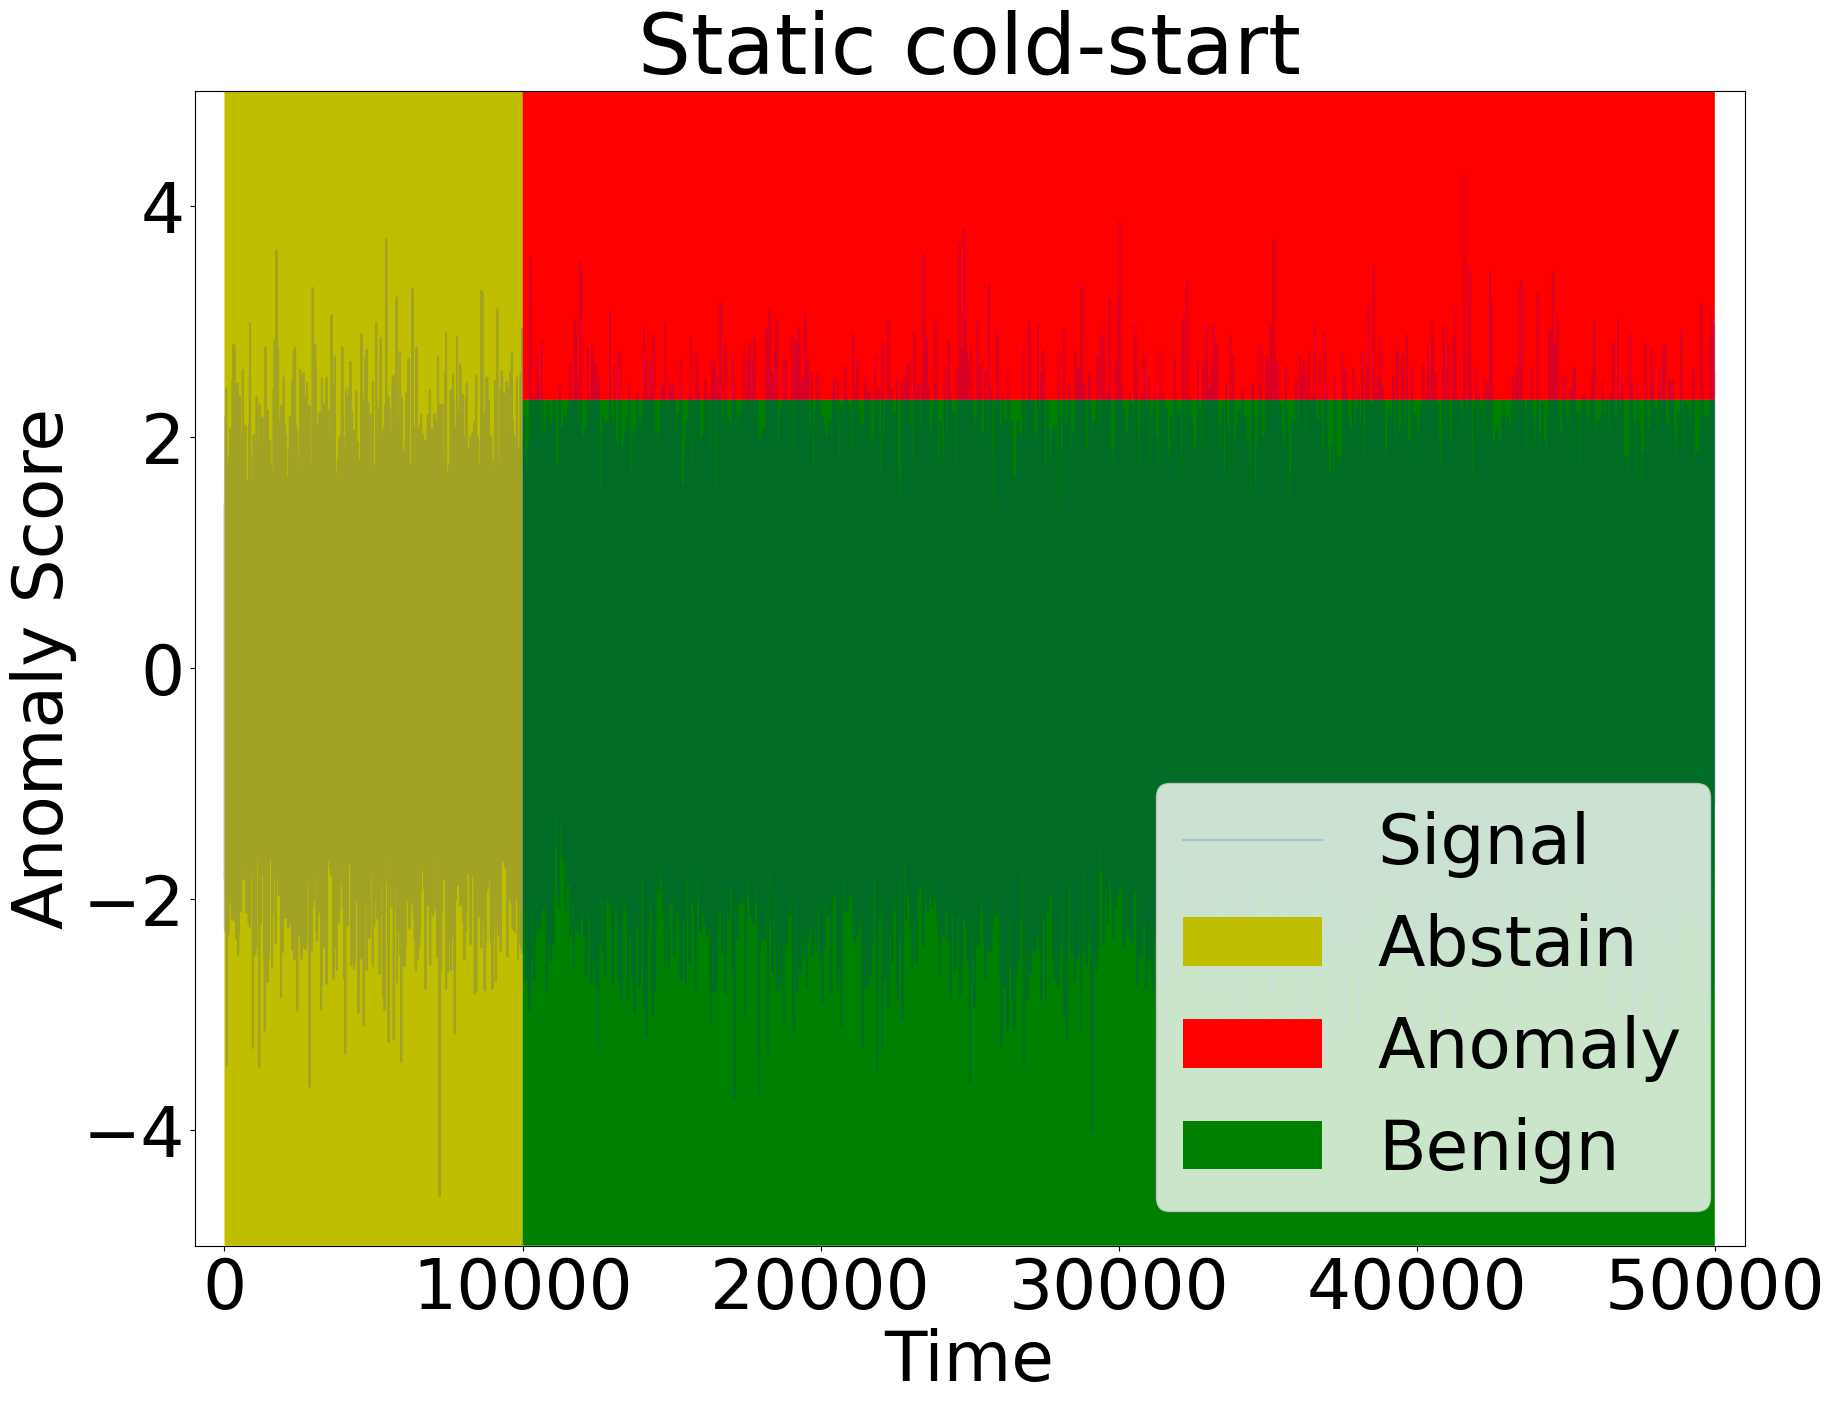
\includegraphics[width=\linewidth]{anomaly/figs/static_cold_start.png}
  %\caption{Anomaly threshold set using a fixed cold-start period}
  \caption{}
  \label{fig:static_cold_start}
\end{subfigure}%
\begin{subfigure}{.48\columnwidth}
  \centering
  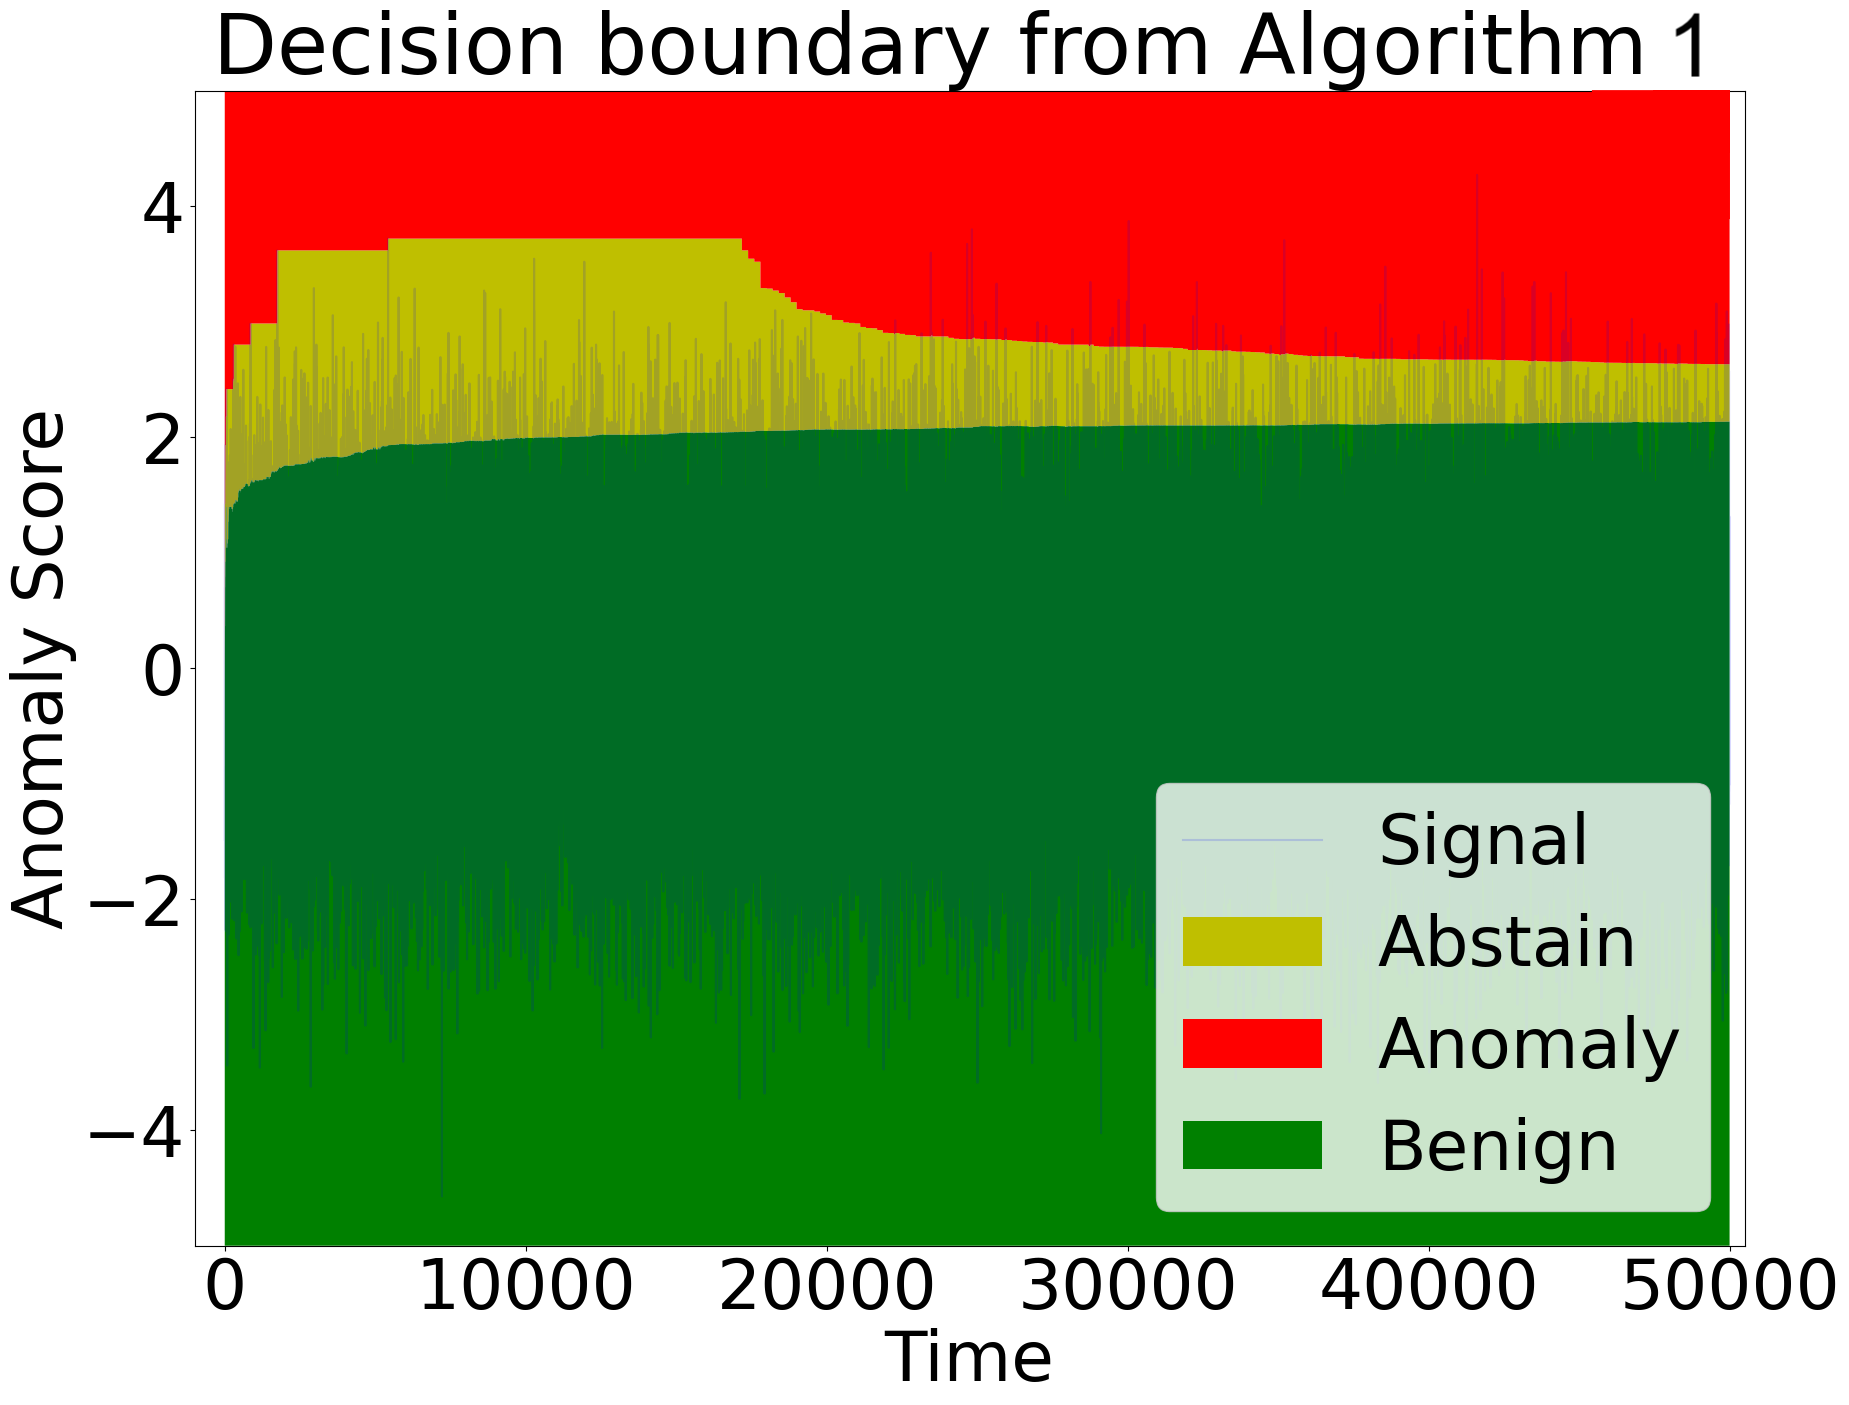
\includegraphics[width=\linewidth]{anomaly/figs/algo1_example.png}
  %\caption{A subfigure}
  \caption{}
  \label{fig:sub2}
\end{subfigure}
\vspace{-0.5em}
\caption{Fig $(a)$ is the heuristic of a fixed cold-start where all samples are abstained from and a static threshold for all future samples. Fig $(b)$ is the decision boundary from Algorithm \ref{alg:one} using an adaptive cold-start.}
\label{fig:motivation_alg_1}
\vspace{-1.5em}
\end{figure}





% AD algorithms abstain by relying on an initial cold-start period. At the end of the cold-start period, the AD system will use the samples seen and any offline information to choose an appropriate threshold \cite{audibert2020usad, chandola2009anomaly}. 




% We introduce abstaining as a possible output of an AD algorithm, in addition to the canonically binary output of anomaly and benign data. The abstain option can be viewed as a data-adaptive, more flexible framework of the cold start period that is commonly used to tune the anomaly threshold. In this paper we include abstaining into the regret metric, to analyze its trade off with making false positive and false negative errors.  

% \paragraph{Leveraging offline datasets to improve online performance, provably}


% \paragraph{Finite-sample, distribution free guarantees on performance}

% \paragraph{Contributions} We are the first work to systematically study the problem of unsupervised anomaly thresholding. We propose algorithms in various settings, and provide a principled framework to analyze their performance. Our contributions are: 

% \begin{enumerate}
% \item {\color{red} Our method provides a statistical framework to tune anomaly thresholds in an online fashion. Our methodology picks a `cold-start' period that is data dependent. Anomalies that are harder to distinguish have a larger cold-start than those that are easier to distinguish.
% Thus, our methodology gives a principled generalization of the common heuristic of having a fixed cold-start period. }
%     %\item Our algorithm improves upon the manually tuned anomaly thresholding with cold-start period commonly used in practice, and provide an algorithm where abstaining is adaptive and data-dependent.
%     \item We prove guarantees on false positive and false negative rates, and number of abstains. {\color{red} 1-2 sentences on the novelty/difficulty}
%     \item We prove that our algorithms and guarantees are adaptive to online distribution shifts. {\color{red}1-2 sentences on how we connect the detection delay with the mistake bounds.}
%     \item Our algorithms leverages offline data to improve online performance with best of both worlds results: it significantly lowers number of abstains when offline data is available, and reduces to online algorithm when it is not. {\color{red} Our algorithm is the first to rigorously show the best of both worlds for online threshold selection?}
% \end{enumerate}

%Our work shows how to tune parameters to achieve. We also show conditions when presence of offline data can improve online performance.....



% \section{Related Work}%\vspace{-0.5em}
% \paragraph{Dynamic thresholding for AD.} AD is an extensively researched topic, where a common paradigm is to first model data likelihood and then use a threshold to decide if a data point is normal or anomalous. This threshold is typically determined by an expert or empirically, see surveys \cite{luo2021deep, schmidl2022anomaly}. Dynamic and automatic methods makes AD algorithms more practical in real-world deployment \cite{ali2013automated, hundman2018detecting}, and are necessary where the data distribution can shift \cite{siffer2017anomaly}. 

% %\cite{siffer2017anomaly, , hundman2018detecting}
% %This work instead focuses on providing a principled analysis of the thresholding step that follows. Traditionally, and are chosen by heuristics . Works closer to us are thresholding algorithms for univariate online streams .
% %\vspace{-0.5em}
% \paragraph{Confidence Sequences.} We use theoretical results and tools of confidence sequences (CS) for our analysis \cite{ramdas2022game}. \cite{maharaj2023anytime, howard2022sequential} derived the CS algorithm for estimating quantiles online with any-time guarantees, and \cite{shekhar2023sequential} leverages CS's consistency property for detecting distribution shifts. These tools allows us to bound the false positive and negative rates of our algorithm.

% {\color{red} \paragraph{Threshold learning systems.}
% Threshold scores to make the binary decision have been studied in active learning to make the decision of  seeking labels from experts \cite{balcan2007margin, zhang2016online,vishwakarma2023promises}. However, active learning does not have a concept of mistakes and is thus different from ours. 

% }

\section{Notations and Problem Formulation}

We formally state the problem and performance measures.
\vspace{-0.6em}

\subsection{Online Data Stream}
\label{subsec:online_data_stream}

A data-stream of length $T \in \mathbb{N}$ is a collection of $T$, independent, scalar valued random variables $(S_t)_{t=1}^T$, indexed by time $t \in [T]$ \footnote{For any positive integer $L$, we denote $[L] = \{1,\cdots,L\}$}. In practice, $S_t \in \mathbb{R}$ at time $t$ is the \emph{anomaly score} of an input sample produced by an AD algorithm such that high scores corresponds to anomalies.
For each time $t \in [T]$,  $f_t$ is the probability distribution of $S_t$, i.e., $S_t \sim f_t$. We assume $f_t$ is a continuous measure without discrete atoms.\footnote{Formally, $\forall p \in (0,1)$, the set $\{ Q \in \mathbb{R}: \mathbb{P}_{X \sim f}[X \leq Q] = p\}$ has exactly one element.} Since the distribution $f_t$ is indexed by time $t$, $(S_t)_{t=1}^T$ is not necessarily identically distributed and thus non-stationary. We assume that the data-stream although is non-stationary, is piece-wise stationary. 

\begin{definition}(Piece-wise stationary) Let $T$ be the time horizon and let $H_T \leq T-1$ be the total number of change points. Define a set of strictly increasing time indices  $1 < \tau_1 < \tau_2 \cdots < \tau_{H_T}$ as change points; let $\tau_0 = 0$ and $ \tau_{H_T+1} = T$. A piece-wise stationary data-stream $(S_t)_{t=1}^T\sim\Bigl(T,H_T, (\tau_c)_{c=0}^{H_T}, (f^{(c)})_{c=0}^{H_T}\Bigr)$ is such that $\forall k \in [1, H_T]$:
\begin{itemize}[noitemsep,topsep=-2pt,labelwidth=!, labelindent=0pt]
   \item $\forall t \in [\tau_k,\tau_{k+1})$, $S_t \sim f^{(k)}$ are i.i.d. with the $p$-quantile of $f^{(k)}$ denoted as $ Q^{(k)}(p) \in \mathbb{R}$. %Thus, $\forall t \in [\tau_k,\tau_{k+1})$, 
    \item  $f^{(k)} \neq f^{(k+1)}$
\end{itemize}
\label{def:piecewise}
\end{definition}

\begin{figure}[h!]
    \centering
    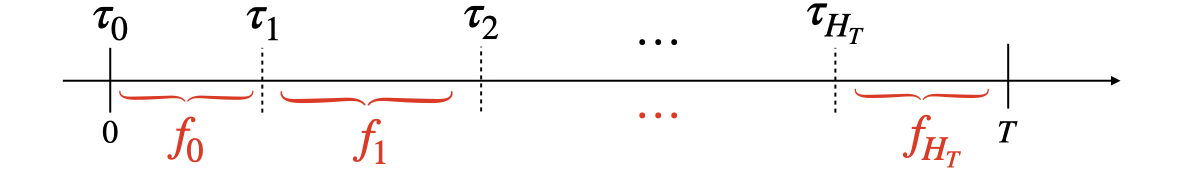
\includegraphics[width=0.9\linewidth]{anomaly/figs/piecewise.jpeg}
    \caption{The piece-wise stationary process}
    \label{fig:enter-label}
    \vspace{-0.8em}
\end{figure}

The special case of $H_T = 0$ corresponds to a stationary i.i.d. data stream.
We remark that our algorithm does not have any information on the change-points  $H_T$, $(\tau_t)_{t=1}^{H_T}$, nor on distributions $(f^{(c)})_{c=0}^{H_T}$. %Nevertheless, the performance  of our algorithm will adapt with the complexity of the data-stream. 

\subsection{Anomaly Definition} 
\label{subsec:anomaly_defn}
%
%As is standard, anomalies are as those time points where the observed sample $S_t$ is larger than the $p$th quantile.
%Following convention \cite{chandola2009anomaly}, we will assume that large values of scores are anomalies. 

\begin{definition}[Anomalies] 
The sample $S_t \sim f_t$ at time $t$ is an anomaly if $S_t > \tau_t$, where $\tau_{t} = \inf \{ \tau\geq 0: \mathbb{P}_{S \sim f_t}[S \leq \tau] \geq p \}$ and $p \in (0,1)$. We denote by $y_t = \mathbf{1}(S_t > \tau_t)$ the indicator variable that the sample $S_t$ is an anomaly.
% \begin{align}
% \begin{split}
%    y_t &= \mathbf{1}(X_t > \tau_{p} ), \text{where} \\
%     \tau_{p} &= \inf \{ \tau\geq 0: \mathbb{P}_{X_t \sim f_t}[X_t \leq \tau] \geq p \}
% \end{split} 
% \end{align} 
\label{def:anomaly}
\end{definition}
%\vspace{-1em}
In words, a sample $S_t$ is anomalous if it exceeds the threshold $\tau_t$ corresponding to the $p$th quantile. Thus, the thresholding algorithm needs to estimate $\tau_t$ and then use that estimate to make the binary decision of whether $S_t$ is an anomaly.
We assume the quantile value $p \in (0,1)$ to be known. 
%In practice, knowledge of $p$ arises, either from constraints on the rate of anomalies that can be investigated \cite{hassan2019nodoze, ho2021hopper}, or from domain knowledge on the base rate of anomalies \cite{perini2023unsupervised}.
% and is thus an extrinsic input.  %While this paper is motivated by anomaly detection and thus focuses on extreme values on one side, but our definitions and algorithms can easily be modified to detect anomaly on both sides, by simultaneously estimating a low and a high quantile.

\subsection{Offline Datasets}
\label{subsec:offline_datasets}

We formalize the notion of \emph{offline datasets} that can be used in addition to using historical samples on the data-stream. Offline datasets are typically available to train the anomaly scoring systems \cite{bhatia2022memstream, audibert2020usad} and have been used to address the cold-start problem in previous works \cite{gutflaish2019temporal,hofmann1999probabilistic}.


 \begin{definition}[Offline Dataset] We define an offline dataset as $K$ sets of independent samples $\mathcal{D} := \{\{X_i^{(j)}\}_{i=1}^{N_j} \}_{j=1}^K$. Each $j \in \{1,\cdots,K\}$ set $\{X_i^{(j)}\}_{i=1}^{N_j}$  are independent samples such that all of the $N_j$ samples are drawn from distributions having the same $p$th quantile denoted by $Q_{(j)}(p)$. A special case is $\{X_i^{(j)}\}_{i=1}^{N_j}$ are i.i.d., with all $N_j$ samples having identical distributions and thus identical $p$th quantile.
 \label{definition:offline_dataset}
 \end{definition}

Observe that $\mathcal{D} = \emptyset$ corresponds to the special case of no offline data availabe.
We will assume that $K$, the number of partitions are known to the algorithm. Clustered offline datasets is a valid assumption, since typically, the offline data is pre-processed before deploying online algorithms. In practice, the clusters could correspond to different groups of signals, e.g. different sensor types, different environmental conditions or day of the week \cite{khan2020industrial, audibert2020usad, sadik2014research}. 

\subsection{Online Anomaly Thresholding Algorithm}
\label{subsec:oad_algo_defn}
 
\begin{definition} An online anomaly thresholding algorithm $\gA$ outputs a label  $\hat{y}_t = \mathcal{A} (S_t; (S_1, \ldots,S_{t-1}), \mathcal{D})\in \{0,1,* (\text{abstain})\}$, a decision for the score $S_t$ depending on the history $S_1, \cdots, S_{t-1}$ and offline datasets $\mathcal{D}$ if any. 
\label{def:algo}
\end{definition}

We emphasize the dependence on the offline dataset $\mathcal{D}$ in the algorithm since that can be used to make a decision at all times. 
However, as mentioned before, the algorithm has no information about the data-stream quadruple, nor any parametric information on the distribution from which either the scores $(S_t)_{t=1}^T$ or the offline dataset $\mathcal{D}$ are sampled from. 
% Since we are interested in assessing the online performance, we make this assumption that the offline dataset is perfectly clustered. We defer the effect of imperfections in the offline data on the online performance to the future.

% \begin{itemize}
%     \item No assumptions on underlying distributions, i.e., $f_t \in \mathcal{M}$ for all $t$.
%     \item small number of mistakes (false positives and false negatives), sub-linear growth of abstains.    
%     \item The performance guarantees are adaptive to small number of distribution shifts in the stream.
%     \item In the presence of a offline dataset: If the test stream is similar to the dataset, then we want to leverage the past and yield improved results. 
%     \item  If the test online stream is arbitrary, then we do not want the online performance to be arbitrarily bad - rather it should be comparable to standard online algorithms that does not assume prior knowledge. 
% \end{itemize}

\subsection{Performance Measures}
\label{subsec:performance_defnition}

The three performance measures of an anomaly thresholding algorithm are {\em (i)} False Positives $\text{FP} = \sum_{t=1}^T \mathbf{1}(\hat{y}_1 = 1, y_t = 0)$, {\em (ii) } False Negatives $ \text{FN} = \sum_{t=1}^T \mathbf{1}(\hat{y}_0 = 1, y_t = 1)$, and {\em (iii)} $\text{Abstains} = \sum_{t=1}^T \mathbf{1}(\hat{y}_t = *)$. We
denote by $\text{Mistakes} := \text{FP} + \text{FN}$ as the sum of false-positives and negatives. The desiderata of high-accuracy and low abstains translate to having a constant independent of $T$ mistakes and a sub-linear in $T$ abstains. 


\section{Lower Bound: Achieving high accuracy requires abstaining}
%
Choosing thresholds for online anomaly detection is non-trivial.
In the absence of abstaining, the expected sum of FPs and FNs is at-least order $\sqrt{T}$ on an i.i.d. stream. We provide a sketch and defer details to the Appendix. Consider the standard reduction of estimation to hypothesis testing \cite{wainwright2019high} where the stream is either coming from the standard gaussian or a unit variance gaussian with mean located at $\frac{1}{\sqrt{T}}$. Denote by $Q^{(0)}(p) < Q^{(1)}(p)$ to be the $p$th quantile of the two distributions respectively. Lower bounds from hypothesis testing gives that at any test that looks at all $T$ samples and identifies which of the two distributions the stream came from makes a mistake with probability at-least $1/8$. Furthermore, Chernoff bound applied to the binary random variables $\mathbf{1}_{Q^{(0)}(p) < S_t < Q^{(1)}(p)}$ gives that with probability at-least $1-e^{\sqrt{T}/8}$, at-least ${C_p\sqrt{T}}$ samples among $S_1, \cdots, S_T$ lies in the range $[Q^{(0)}(p), Q^{(1)}(p)]$, where $C_p$ is a constant depending on $p$. Thus, an union bound gives that in the absence of abstains, with probability at-least $1/8-e^{\sqrt{T}/8}$, the sum of FP and FN is at-least ${C_p\sqrt{T}}$. A formal statement and proof in Section \ref{sec:lower_bound_proof} in the Appendix.


\section{Special Case I: Stationary stream only} %without offline data}% Stationary stream}
In order to build up the intuition and concepts, we consider three special cases in increasing order of complexity {\em (i)} stationary stream without offline data {\em (ii)} piece-wise stationary stream {without offline dataset}, and {\em (iii)} stationary stream with offline dataset. The  ideas from these special cases are developed in Section \ref{sec:general_setting} to give the general algorithm. 
%\subsection{Stationary stream with no offline data}


In this section, we consider the special case when the online algorithm knows that data-stream $(S_t)_{t\geq 1}$ is an i.i.d. sequence and there is no offline dataset for warm-starting, i.e., $\mathcal{D} = \emptyset$. For this special case, we show in Theorem \ref{the:iid} that results from \cite{howard2022sequential} yields an algorithm that guarantees $0$ mistakes and $\mathcal{O}(\sqrt{T})$ abstains.
%with high probability. 
%This special case is further sub-divided into two settings - {\em (i)} the case when there is no offline dataset, i.e., $\mathcal{D} = \emptyset$, and {\em (ii)} the case when there is offline dataset to wram-start the online algorithm.
%For this simple setting, our goal is straightforward - we want to make close to 0 mistakes without incurring too many abstains. To achieve such goal, we introduce the anytime-valid confidence sequences (CS) algorithm introduced in \cite{howard2022sequential}.  

To formally state the results, we set notations. For any sequence of numbers $(y_t)_{t \geq 1}$ and $t_1 < t_2$, denote by $y_{t_1:t_2}:= (y_{t_1}, \cdots,y_{t_2})$. For a positive integer $t$, sequence $y_{1:t}$, and $p \in (0,1)$, the $p$th empirical quantile of $y_{1:t}$ is given by $\widehat{Q}(p; y_{1:t}) := \frac{y^{(\lfloor pt \rfloor)} + y^{(\lceil pt \rceil)}}{2}$, where $y^{(1)} \leq \cdots \leq y^{(t)}$ is the sorted order of $y_{1:t}$. 

\begin{definition}[Confidence Sequences (CS) of a quantile] For $\alpha \in (0,1)$, a level $1-\alpha$ CS of the $p \in (0,1)$ quantile of an i.i.d. sequence $(S_t)_{t\geq 1}$ with true $p$th quantile $Q(p) \in \mathbb{R}$, is a collection of subsets $\{ C_t: t\geq 1\}$ such that for all $t\geq 1$, {\em(i)} $C_t \subseteq \mathbb{R}$,  {\em (ii)}  $C_t$ is $\sigma(S_1, \ldots, S_t)$-measurable w.r.t. the first $t$ samples  and {\em (iii)} $\prob( Q(p) \in \bigcap_{t \geq 1} C_t) \geq 1-\alpha$.
\label{defn:CS}
\end{definition}

%\subsection{Stationary stream and no offline data}

% \subsection{Closed form for a quantile CS}

%We use the results in \cite{howard2022sequential} and use an explicit closed form for a CS. 
%In order to give a closed form expression for a CS, 



\begin{theorem}[Theorem 2 from \cite{howard2022sequential}]
    Let $(S_t)_{t \geq 1}$ be an i.i.d. sequence of $\mathbb{R}$ valued random variables. Given $\alpha \in (0,1)$, for all $p \in (0,1)$, the sequence of sets $(C(p,\alpha,S_{1:t}))_{t \geq 1}$ is a $1-\alpha$ level CS for the $p$th quantile, where for any sequence of numbers $(y_{1:n}) $, %$C(p,\alpha,y_{1:n}) \subseteq \mathbb{R}$ is defined as
        \begin{multline}
        C(p, \alpha, y_{1:n}) = \bigg[ \widehat{Q}(\max(p-2u_{n}(\alpha),0), y_{1:n}), \widehat{Q}(\min(p+2u_{n}(\alpha),1), y_{1:n}) \bigg],
        \label{eq:cs}
   \end{multline}
    % \begin{multline}
    %     C(p, \alpha, S_{1:t}) = \bigg[ \widehat{Q}(p-u_t(\alpha); S_{1:t}),  \\  \widehat{Q}(p+u_t(\alpha); S_{1:t}) \bigg],
    %         \label{eq:cs}
    % \end{multline}
    where $u_{(\cdot)}(\cdot): \mathbb{N} \times [0,1] \to [0,1]$ given by the function 
    \begin{align}
       u_t(\alpha) = 0.85 \sqrt{t^{-1}[\log\log(et) + 0.8 \log(1612/\alpha)]},
       \label{eqn:defn_confidence_width_ut}
    \end{align}
    and for all $\alpha \in [0,1]$, $u_0(\alpha) = 1$.
\end{theorem}

% For brevity, we will use the notation $CS({S_1, \ldots, S_T}) = \{ C_t: t\geq 1\}$ to describe the procedure of obtain a confidence sequence from a data stream ${S_1, \ldots, S_t}$. For a given confidence level $p$, we calculate $C_t$ as:
% \begin{equation}
%     C_t = [ \hat{Q}_t(p - u_t), \hat{Q}_t(p+u_t)] \quad \text{where} 
%     \label{eq:cs}
% \end{equation} 
% \begin{equation}
% u_t = 0.85 \sqrt{t^{-1} [\log\log(et) + 0.8 \log(1612/\alpha)]}
% \label{eqn:defn_confidence_width_ut}
% \end{equation}
% where $\hat{Q}$ is the empirical quantile function. 



A thresholding algorithm for this special case is obtained from the definition of CS as shown in Algorithm \ref{alg:marginal_decision}. 
%The complete pseudo-code is in Algo. \ref{alg:one} in the Appendix with the following performance guarantee. 


% \begin{algorithm}
% \caption{OAD for stationary i.i.d. stream}\label{alg:one}
% \SetKwInOut{Input}{Input}
% \SetKwInOut{Output}{Output}
% \Input{Quantile $p$, Confidence $1-\alpha$}
% \Output{Anomaly labels $\hat{y}_1, \hat{y}_2, \ldots$}
% \For{  $\text{each time }t \geq 1$ } {
%     Receive $t^{th}$ input $S_t$\;
%     Compute $lb_t$ and $ub_t$ (Eq. \ref{eq:cs})\;
%     %Compute $ub_t \gets \hat{Q}_t(p + u_t)$(Eq. \ref{eq:cs})\; 
%     \uIf{$S_t > ub_t$}{
%     $\hat{y}_t \gets1$\;
%   }
%   \uElseIf{$lb_t \leq S_t \leq ub_t $}{
%   $\hat{y}_t \gets * $ \;
%   }
%   \Else{
%     $\hat{y}_t \gets 0 $ \;
%   }
% }
% \end{algorithm}

% \subsection{Mistake and abstain bound for stationary streams}
% The desiderata of our problem consists of three parts, false positives/negatives and abstains. We will analyze them in order respectively. We first define our good event as follows:
% %
% \begin{definition}[Good event $\gE_1$] %Denote the good event $\mathcal{E}_1$ as 
% \begin{align}
% \begin{split}
%     \mathcal{E}_1 := \bigcap_{t \in \mathbb{N}} \bigcap_{p \in (0,1)} 
%    \bigl(  &  \{ Q(p) \leq \widehat{Q}_t(p+u_t) \} \\
%     & \bigcap \{ Q(p) \geq \widehat{Q}_t(p-u_t) \} \bigr).
% \end{split}
% \label{eqn:good_event_defn}
% \end{align}   
% \end{definition}
% %
% In words, the good event states that for all time $t$, the confidence sequence contains the true $p$th quantile.
% From Corollary $2$ of \cite{howard2022sequential}, we know that $\mathbb{P}[\mathcal{E}] \geq 1-\alpha$. We remark that \cite{howard2022sequential} show that even when $(S_t)_{t \geq 1}$ are independent, but not necessarily identical, $\mathbb{P}[\mathcal{E}] \geq 1-\alpha$ holds as long as the $p$th quantile $Q_t(p) := Q(p)$ for all $t \geq 1$. This extension relaxing the identical distribution will be crucial in the subsequent sections in the sequel. 


\begin{algorithm}
\caption{Decision making with confidence set}\label{alg:marginal_decision}
\SetKwInOut{Input}{Input}
\SetKwInOut{Output}{Output}
\Input{Sample $S \in \mathbb{R}$, Confidence set $C \subseteq \mathbb{R}$ }
\Output{Anomaly label $\hat{y} \in \{0,1,*\}$}

    \uIf{$S > \max C$}{
    $\hat{y} \gets1$ \tcp{Declare an anomaly}
  }
  \uElseIf{$S \in C$}{
  $\hat{y} \gets * $  \tcp{Abstain from decision}
  }
  \Else{
    $\hat{y} \gets 0 $  \tcp{Declare benign}
  }
  \Return $\hat{y}$
  

\end{algorithm}

\begin{theorem}
Suppose for an i.i.d., data-stream $(S_t)_{t\geq 1}$, the decision at time $t$ is given by the output of Algorithm \ref{alg:marginal_decision} with inputs $S_t$ and confidence $C(p,\alpha, S_{1:t-1})$. Then, with probability at-least $1-2\alpha$, $0$ mistakes and at-most $7 \sqrt{T \ln \left( \frac{1612\ln(eT)}{\alpha^2} \right)}$ abstains are incurred. 
% \begin{enumerate}[noitemsep,topsep=-2pt,labelwidth=!, labelindent=0pt]
%     \item $0$ False positives, $0$ False negatives
%     \item Less than or equal to 
% \end{enumerate}
\label{the:iid}
\end{theorem}

\begin{remark}
   Theorem \ref{the:iid}  implies that points $1$ and $2$ from Section \ref{sec:desiderata} are satisfied by Algorithm \ref{alg:one}.
    \end{remark}



\begin{remark}
   To bound the number of abstains, we need a different analysis compared to \cite{howard2022sequential} to control the probability that a sample $S_{t}$ lies within $C(p,\alpha, S_{1:t-1})$. We do this by constructing a martingale from the sequence of binary random variables $\mathbf{1}_{S_t \in C(p,\alpha, S_{1:t-1})}$ and applying Azuma's inequality. %To do so, we needed the extra factor of $2$ in front of the $u_n(\alpha)$ function in Equation (\ref{eq:cs}). In fact, \cite{howard2022sequential} showed that Equation (\ref{eq:cs}) without the factor of $2$ is also a $1-\alpha$ CS for the quantile. We needed the extra factor to prove high probability lower bound. See also discussion following Equation (\ref{eqn:good_event_defn}) in the appendix. 
\end{remark}




\section{Special Case II: Piece-wise stationary stream without offline data}
\label{sec:offline-only}

% \begin{figure}
%     \centering
%     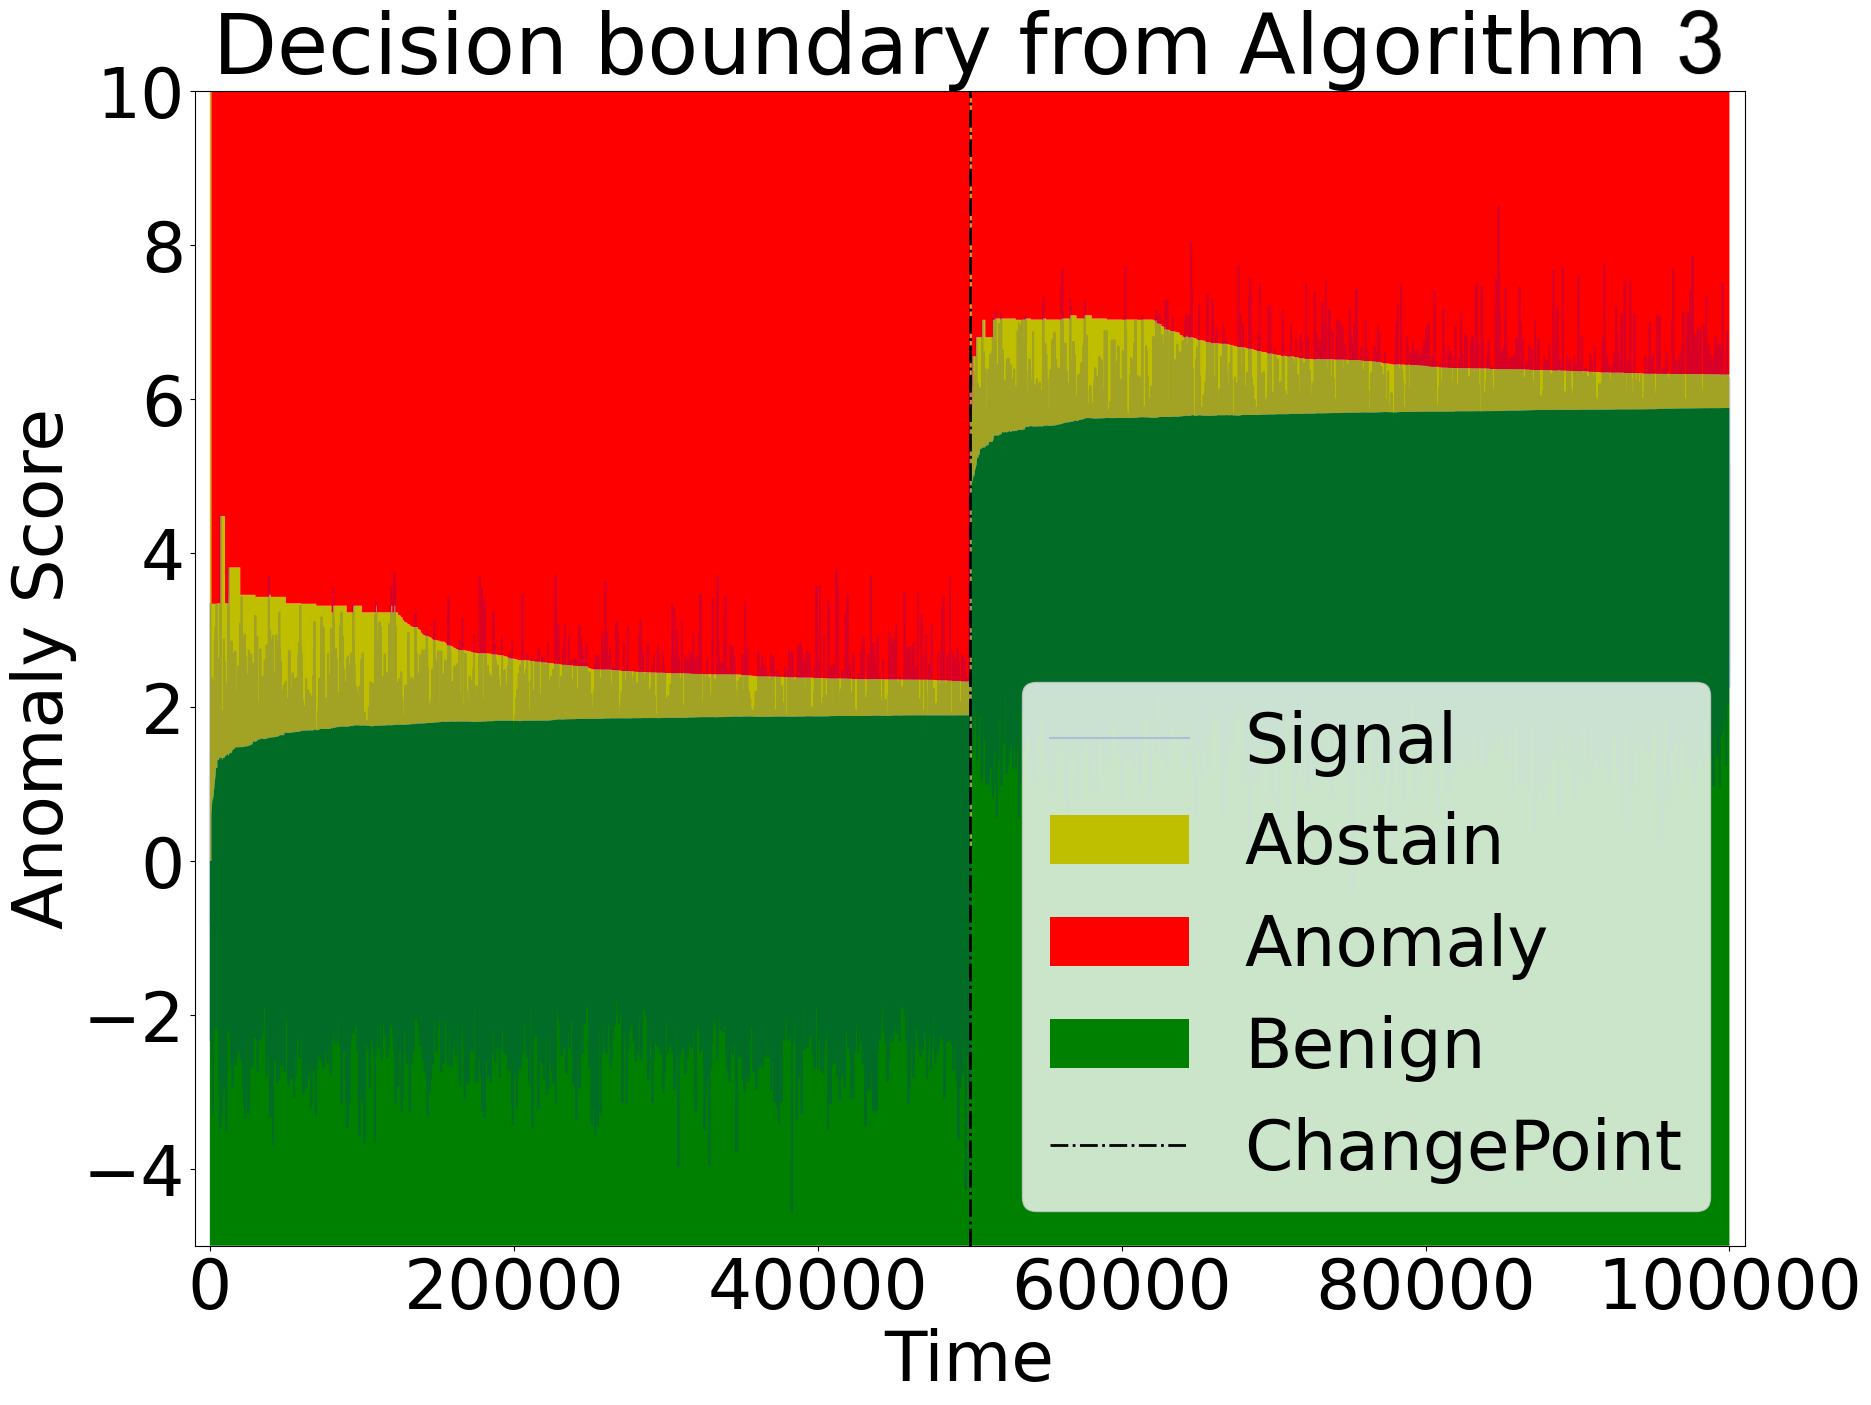
\includegraphics[width=0.55\linewidth]{anomaly/figs/algo_2_example.png}
%     \caption{Algorithm 3 output on a piece-wise stationary stream. \sofi{remake this figure}}
%     \label{fig:s1}
%     \vspace{-1.5em}
% \end{figure}

Going beyond the  i.i.d. case, we consider a piece-wise stationary stream without offline dataset.
Our method in Algorithm \ref{alg:two} uses a change-point detection Algorithm \ref{alg:change_point} from \cite{shekhar2023sequential} as a sub-routine. We need a  definition to state the main result of this section. %Algorithm \ref{alg:change_point} is the forward-backward CS strategy from \cite{shekhar2023sequential}, where a change-point is detected at time $t$, if there exists $1 \leq \tau < t$ with $C(p,\alpha,S_{1:\tau})$ and $C(p,\alpha,S_{\tau+1:t-1})$ having an empty intersection.
% We set additional notation to describe the algorithm. Given the data-stream $(S_t)_{t \geq 1}$ and $t_1 < t_2$ integers, define the set $C(p,\alpha,S_{t_1:t_2})\subseteq \mathbb{R}$ as 
%     \begin{multline}
%         C(p, \alpha, S_{t_1:t_2}) = \bigg[ \widehat{Q}(p-u_{t_2-t_1+1}(\alpha); S_{t_1:t_2}), \\  \widehat{Q}(p+u_{t_2-t_1+1}(\alpha); S_{t_1:t_2}) \bigg].
%         \label{eqn:modified_cs}
%    \end{multline}
% The definition in Equation (\ref{eqn:modified_cs}) is a generalization of the definition in Equation (\ref{eq:cs}) that changes the starting index from $1$ to $t_1$.
%Algorithm \ref{alg:two} detects a change at time $t$, if there exists $1 \leq \tau < t$ such that $C(p,\alpha,S_{1:\tau})$ and $C(p,\alpha,S_{\tau+1:t})$ are non-intersecting, 
%When a change is detected, Algorithm \ref{alg:two} restarts the stationary algorithm. %The full pseudo-code is given in Algorithm \ref{alg:two}. 
%process, a common framework as seen in \cite{sankararaman2023online}.

% \begin{definition}(Piece-wise stationary process) Let $T$ be the time horizon and let $H_T < T$ be the total number of change points. Define a set of strictly increasing time indices  $1 < \tau_1 < \tau_2 \cdots < \tau_{H_T}$ as change points; let $\tau_0 = 0$ and $ \tau_{H_T+1} = T$. The process, $S_1, \cdots, S_T$ is  identified by the quadruple $\Bigl(T,H_T, (\tau_c)_{c=0}^{H_T}, (f_c)_{c=0}^{H_T}\Bigr)$, such that $\forall k \in [1, H_T]$:
% \begin{itemize}[noitemsep,topsep=-3pt,labelwidth=!, labelindent=0pt]
%    \item $\forall t \in [\tau_k,\tau_{k+1})$, $S_t \sim f_k$ i.i.d., with the $p$-quantile of distribution $f_k$ denoted as $ Q_k$
%     \item  $Q_k \neq Q_{k+1}$
% \end{itemize}
% \label{def:piecewise}
% \end{definition}

% \begin{figure}[h!]
%     \centering
%     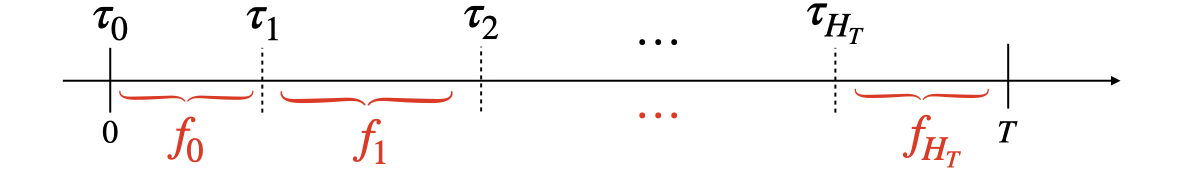
\includegraphics[width=0.9\linewidth]{anomaly/figs/piecewise.jpeg}
%     \caption{The piece-wise stationary process}
%     \label{fig:enter-label}
%     \vspace{-0.8em}
% \end{figure}
 % The anytime-valid property of CSs allows us to bound detection delay and probability of mis-detection, as we show in the following analysis. 


\subsection{Measure of distribution shift}

%We assume all of the distributions in our online stream is \textit{unknown}. In this setting, it is crucial to relate the magnitude of changes (e.g. in our case the shift of quantiles) to the number of available observations between changes \cite{maillard2019sequential}. We therefore introduce some assumptions.

%We define a measure of distribution shift, which dictates the complexity of non-stationarity detection.
%The following is the main definition of distribution shift.

\begin{definition}[quantile shift]
For two continuous distributions $f,g$  on $\mathbb{R}$ with quantile functions  $Q_f(\cdot), Q_g(\cdot) : [0,1] \to \mathbb{R}$ respectively, the distance at quantile $p \in (0,1)$ denoted as $\text{Shift}(f,g,p)$ is defined as
% \begin{multline*}
%     \text{Shift}(f,g,p) := \sup \bigg\{ \Delta \geq 0: \max\bigg[Q_f\left(p-\frac{\Delta}{2}\right) - \\ Q_g\left(p + \frac{\Delta}{2}\right) ,  Q_g\left(p-\frac{\Delta}{2}\right) - Q_f\left(p + \frac{\Delta}{2}\right) \bigg] \geq 0 \bigg\}.
%     \end{multline*}

\begin{multline*}
    \text{Shift}(f,g,p) := \sup \{ \Delta \geq 0: \max[Q_f\left(p-{\Delta}\right) -  Q_g\left(p + {\Delta}\right) ,  Q_g\left(p-{\Delta}\right) - Q_f\left(p + {\Delta}\right) ] \geq 0 \}.
    \end{multline*}
\label{def:quantile_shift}
\end{definition}

Observe that for any two continuous distributions $f$ and $g$, $\text{Shift}(f,g,p) \in [0,1]$ and $\text{Shift}(f,g,p) = 0$ if and only if $f$ and $g$ have identical $p$th quantile. %In words, this definition states that a distribution shift occurs at time $t \geq 2$ if and only if the $p$th quantile at time $t-1$ is different from that at time $t$. 
The following proposition shows that the quantile shift is the non-stationary measure that governs the delay in detecting a change-point.

%We will show in Theorem \ref{thm:online_shift} that the number of FP, FN and abstain guarantees scale this magnitude of distribution shift. %In that regard, Definition \ref{def:quantile_shift} is the most genera; definition since time $t$ is not considered a change point, and thus does not impact performance guarantees, if the distribution at time $t-1$ and $t$ are different, but having identical $p$th quantile.
% %



\begin{algorithm}
\caption{Change detection \cite{shekhar2023sequential}}\label{alg:change_point}
\SetKwInOut{Input}{Input}
\SetKwInOut{Output}{Output}
\Input{$p, \alpha \in (0,1)$, sequence $S_{1:n}$ }
\Output{Binary variable if input has a change-point}

$\widetilde{C} \gets \bigcap_{s \leq n}C(p, \alpha, S_{1:s})$ $\forall t \in [n]$\;

$\widehat{C} \gets \bigcap_{s \leq n}C(p, \alpha, S_{s:n})$ $\forall t \in [n]$\;

\Return $\mathbf{1}( \widetilde{C} \bigcap \widehat{C} = \emptyset)$\: \tcp{1 is a change-point}


\end{algorithm}
 

\begin{algorithm}
\caption{Thresholding without offline data}\label{alg:two}
\SetKwInOut{Input}{Input}
\SetKwInOut{Output}{Output}
\Input{Quantile $p \in (0,1)$, Confidence $\alpha \in (0,1)$}
\Output{Anomaly labels $\hat{y}_1, \hat{y}_2, \ldots$}
$\tau \gets 0$ \tcp*{\small{previous change point}}
\For{  $\text{each time }t \geq 1$ } {
    Receive $t^{th}$ input $S_t$\;
    
    % $\text{forward-CS} \gets CS(\{S_{\tau}, S_{\tau+1}, \ldots, S_t \})$  \;
    
    % $\text{backward-CS} \gets CS(\{ S_t,S_{t-1}, \ldots, S_{\tau} \})$  \;
    
    \uIf{ \text{{\ttfamily Algorithm-}} \ref{alg:change_point} $(p,\alpha,S_{\tau+1:t-1})==1$ }{
    
        $\hat{y}_t \gets * $ \;     \tcp{\small{Change-point detected}}
        
        $\tau \gets t-1$ \;
    }
    \Else{
        $\hat{y}_t \gets$ {{\ttfamily Algorithm-}}\ref{alg:marginal_decision} $(S_t, C(p,\alpha,S_{\tau+1:t-1}))$\;
  }
}
\end{algorithm}


%{\color{red} ---- AS edited till here.}

% \subsection{Good events for quantile estimation}

% \begin{definition}[Good event 2] 
% Let $(S_t)_{t=1}^T \sim \Bigl(T,H_T, (\tau_c)_{c=0}^{H_T}, (f^{(c)})_{c=0}^{H_T}\Bigr)$, with quantile functions of the $H_T+1$ segments given by $(Q^{(c)}(\cdot))_{c=0}^{H_T}$. Define $\gE_2$ as
% \begin{align}
%     \gE_2 := \bigcap_{k=1}^{H_T} \gE_2^{(k)},
%     \label{eqn:good_event_2_defn}
% \end{align}
% where for each $k \in [H_T]$, 
% \begin{multline*}
%         \mathcal{E}_2^{(k)} =  \bigcap_{p \in [0,1]} \bigcap_{t_1 = \tau_{k}}^{\tau_{k+1}} \bigcap_{t_2 = t_1 +1}^{\tau_{k+1}}   \bigg\{ \widehat{Q}(p-u_{t_2 - t_1}(\alpha), S_{t_1:t_2}) \\ \leq Q^{(k)}(p) \leq \widehat{Q}(p-u_{t_2 - t_1}(\alpha), S_{t_1:t_2}) \bigg\},
% \end{multline*}
% where $\widehat{Q}$ is the empirical quantile and $u_{(\cdot)}(\cdot)$ is defined in Equation (\ref{eqn:defn_confidence_width_ut}).
% \label{as:goodevent2}
% \end{definition}
% %\vspace{-1em}
% %
% In words,  $\gE_2$ is the intersection over all the $H_T+1$ stationary segments, where for each segment the quantile estimate is close to the true quantile for all quantiles. Following Corollary $2$ of \cite{howard2022sequential} and an union bound, we get the following.

% \begin{proposition}
%     \begin{align*}
%         \mathbb{P}[\gE_2] \geq 1 - T\alpha.
%     \end{align*}
%     \label{prop:good_event_2_prob}
% \end{proposition}

% \subsection{Change-point detection delay bounds}

% \begin{proposition}[Stream with a single change-point]
% Let $(S_t)_{t=1}^T$ be a piecewise stationary stream with a single change-point, i.e., $H_T = 1$ with the change-point instant $\tau_1 = \tau \in [T]$. Denote by $\Delta := \text{Shift}(f^{(0)}, f^{(1)}, p)$ as the distribution shift magnitude. Denote by $\tau' \in \mathbb{N}$ as the first time when the {\ttfamily if} statement in Algorithm \ref{alg:two} evaluates to {\ttfamily True}, i.e., a change is detected for the first time by Algorithm \ref{alg:two}. Then, under the good event  $\gE_2$  (Definition \ref{as:goodevent2}), 
% \begin{align*}
%     \tau \leq \tau' 
%     &\leq \lceil \inf_{\widetilde{\tau}} \{  u_{\tau}(\alpha) + u_{\widetilde{\tau}-\tau}(\alpha) \leq \Delta \} \rceil,
% \end{align*}
% where $u_t(\alpha)$ is given in Equation (\ref{eqn:defn_confidence_width_ut}). 
% \label{prop:dist_changes}
% \end{proposition}

%This proposition leads to the following simple corollary. %giving a closed form upper bound on the detection delay. 

\begin{proposition}[Stream with a single change-point]
Let $(S_t)_{t=1}^T$ be a piece-wise stationary with one change-point ($H_T = 1$) and quntile shift $\Delta := \text{Shift}(f^{(0)}, f^{(1)}, p) > 0$, at time $\tau_1 = \tau \geq \frac{80}{\Delta^2}\ln \left( \frac{1612}{\alpha \Delta^2}\right)$. Denote by $\tau' \in \mathbb{N}$ as the first time when Algorithm \ref{alg:two} detects a change, i.e., the {\ttfamily if} statement evaluates to {\ttfamily True}. Then, with probability at-least $1-\alpha T$, $ \tau \leq \tau' \leq \tau + \frac{80}{\Delta^2}\ln \left( \frac{1612}{\alpha \Delta^2}\right)$ .
\label{prop:delay_bound}
\end{proposition}

Thus, if there are sufficient pre-change samples, then the change is detected with delay scaling with $\Delta^{-2}$, which is minimax optimal \cite{maillard2019sequential, JMLR:v23:20-1384, shekhar2023sequential}.
As notation, we define detection delay as $D(\cdot, \cdot): [0,1]\times [0,1] \to \mathbb{R}_{+}$ as 
\vspace{-0.1em}
\begin{align}
    D(\Delta,\alpha) := \frac{80}{\Delta^2}\ln \left( \frac{1612}{\alpha \Delta^2}\right). \label{eq:delay_shorthand} 
\end{align}
\vspace{-1.5em}

\subsection{Mistake and abstain bounds}

To give bounds on performance, we make a simplifying assumption that change-points are sufficiently far apart. We refer the readers to Figure \ref{fig:separated_datasets_example} in the appendix for an illustration of the definitions of Assumption \ref{asumption_detectable} and \ref{defn:offline_datasets}.

\begin{assumption}[$\alpha$-detectable]
For a given $\alpha \in (0,1)$, the piece-wise stationary data-stream $(S_t)_{t=1}^T \sim \Bigl(T,H_T, (\tau_c)_{c=0}^{H_T}, (f^{(c)})_{c=0}^{H_T}\Bigr)$ is said to be $\alpha$-detectable if 
% 
\vspace{-0.5em}
\begin{equation*}
    \tau_{k} - \tau_{k-1} \geq \begin{cases}
        D(\Delta_1,\alpha), &k = 1,\\
        D(\Delta_{k-1},\alpha) + D(\Delta_{k},\alpha), &2\leq k\leq H_T\\
        D(\Delta_{H_T}, \alpha), &k=H_T+1
    \end{cases}
\end{equation*}
%     \begin{align*}
%     \tau_{k} - \tau_{k-1} \geq  D(\Delta_{k-1},\alpha) + D(\Delta_{k},\alpha),
% \end{align*}
% and 
% \begin{align*}
%     \tau_1 \geq D(\Delta_1, \alpha),
% \end{align*}
% and
% \begin{align*}
%    T -  \tau_{H_T} \geq D(\Delta_{H_T}, \alpha),
% \end{align*}
holds, where $\Delta_{k} = \text{Shift} (f^{(k)},f^{(k-1)},p)$.%  is the quantile shift for all $k \in [H_T]$ given in Definition (\ref{def:quantile_shift}) and $D(\cdot,\cdot)$ is defined in Equation (\ref{eq:delay_shorthand}).
\label{asumption_detectable}
\end{assumption}

% Assumption \ref{asumption_detectable} implies that change-points are sufficiently far apart. 
 %We show in Lemma \ref{lem:bdd_delay_change_induction} that under this assumption, all change points are detected Algorithm \ref{alg:two}. 

 This assumption is standard to give guarantees for online algorithms with multiple change points on the stream \cite{JMLR:v23:20-1384, sankararaman2023online, cao2019nearly, liu2018change}. Assumption \ref{asumption_detectable} is made for mathematical tractability and is not assumed in experiments. Analysis without Assumption \ref{asumption_detectable} is an open problem (Section $7$ \cite{JMLR:v23:20-1384}). The main result in this section is Theorem \ref{thm:online_shift}.

% \begin{proposition}[Change-point false positives]
%     Let $(S_t)_{t = 1}^T$ be generated from a piece-wise stationary process satisfying Assumption \ref{asumption_detectable} for $\alpha \in (0,1)$. Then, under the good event $\gE_2$, between any two successive detected change-points in Algorithm \ref{alg:change_point}, there exists exactly one true change-point. 
%     \label{prop:cp_fp}
% \end{proposition}

% Proposition \ref{prop:cp_fp} in conjunction with Corollary \ref{prop:delay_bound} gives that under Assumption \ref{asumption_detectable}, if the good event $\gE_2$ holds, then an instance of the stationary algorithm is re-started within a given delay of a true change occurring. This leads to the following performance guarantee on Algorithm \ref{alg:change_point}. 

% {\color{blue}
% \begin{lemma}[Detectability]  If the good event $\mathcal{E}_2$ holds, then the detection delay for a quantile shift of magnitude $\Delta_{(k)}$ is bounded by
% \begin{align}
%     D(\Delta_{(k)},\alpha) = \frac{20}{\Delta_{(k)}^2}\ln \left( \frac{1612}{\alpha \Delta_{(k)}^2}\right). \label{eq:delay_shorthand} 
% \end{align}
% \label{lem:delay}
% \end{lemma}

% \begin{assumption}[All changes are detectable]
% We will assume that the time-interval between change-points are sufficiently far away. Formally, we will assume that for all change-points $1 \leq k \leq H_T$,  
% \begin{align*}
%     \tau_{k} - \tau_{k-1} \geq \max \left( D(\Delta_{k-1},\alpha) , D(\Delta_{k},\alpha) \right)
% \end{align*}
% where for brevity we denote $\Delta_{k} = Shift (f_{k},f_{k+1})$ as defined in definition \ref{def:quantile_shift}.
% \label{as:changes_detectable}
% \end{assumption}
% }

\begin{theorem}[\textbf{main result for Algorithm \ref{alg:two}}]
Let $(S_t)_{t = 1}^T \sim \Bigl(T,H_T, (\tau_c)_{c=0}^{H_T}, (f_c)_{c=0}^{H_T}\Bigr)$ be  a piece-wise stationary data-stream satisfying Assumption \ref{asumption_detectable} for $\alpha \in (0,1)$. Then, with probability at-least $1-2\alpha T$,  Algorithm \ref{alg:two} satisfies {\em both} 
%{\em (i)} $\text{FP} + \text{FN}  \leq \sum_{k=1}^{H_T}D(\Delta_{k},\alpha)$, and {\em (ii)} Number of abstains $ \leq \sum_{k=1}^{H_T} \Bigl[ 7 \sqrt{(\tau_k-\tau_{k-1}) \ln \left( \frac{1612}{\alpha^2} \ln(3(\tau_k-\tau_{k-1})) \right)}  + D(\Delta_{k},\alpha) \Bigr]$,
\begin{itemize}
    \item   $\text{FP} + \text{FN}  \leq \sum_{k=1}^{H_T}D(\Delta_{k},\alpha)$ %$ = H_T \cdot {\gO}(\frac{1}{(\min_k\Delta_{k})^2}) $\footnote{$\mathcal{O}(\cdot)$ ignores constants and poly-log terms in $\frac{T}{\alpha}$.}
    \item abstains $\leq
     \sum_{k=1}^{H_T} \Bigl[ 4 \sqrt{(\tau_k-\tau_{k-1}) \ln \left( \frac{1612}{\alpha^2} \ln(3(\tau_k-\tau_{k-1})) \right)} + D(\Delta_{k},\alpha) \Bigr]$
\end{itemize}
where for all $k \in [H_T]$, $\Delta_{k} = \text{Shift} (f^{(k)},f^{(k-1)},p)$  is the quantile shift defined in Definition (\ref{def:quantile_shift}) and $D(\cdot,\cdot)$ is defined in Equation (\ref{eq:delay_shorthand}).
\label{thm:online_shift}
\end{theorem}



\begin{remark}
    This result shows that $\text{FP}+\text{FN} =  H_T \cdot {\gO}(\frac{1}{(\min_k\Delta_{k})^2}) $\footnote{$\mathcal{O}(\cdot)$ ignores constants and poly-log terms in $\frac{T}{\alpha}$.},  scales only with the number of changes $H_T$, and  abstains at-most $O(\sqrt{H_TT})$ \footnote{Bound follows from Cauchy-Schwartz inequality that $\sqrt{x} + \sqrt{y} \leq \sqrt{2(x+y)}$, $\forall x,y \geq 0$.}. Thus, desiderata $3$ from Section \ref{sec:desiderata} is achieved.  %The bound on abstains 
\end{remark}

{\color{black}
\begin{remark}
      The bound in Theorem \ref{thm:online_shift} holds with probability $1-2\alpha T$. If $(S_t)_{t=1}^T$ is $\alpha/T$-detectable according to Assumption \ref{asumption_detectable}, and with knowledge of $T$, then Algorithm \ref{alg:two} run with input $\alpha/T$ instead of $\alpha$ yields the same order-wise guarantees as Theorem \ref{thm:online_shift} holding with probability $1-2\alpha$. Corollary \ref{cor:weaker_assumption} in the Appendix shows that assuming $(S_t)_{t=1}^T$ being $\alpha/T$ detectable is only weaker by a logarithmic factor compared to the assumption of $\alpha$-detectable.
\end{remark}

% \begin{corollary}
%     For a given $\alpha \in (0,1)$, $T \in \mathbb{N}$, $H_T \leq T-1$ and distributions $(f^{(c)})_{c=0}^{H_T}$, if $\Bigl(T,H_T, (\tau_c)_{c=0}^{H_T}, (f^{(c)})_{c=0}^{H_T}\Bigr)$ is $\alpha$-detectable according to Assumption \ref{asumption_detectable}, then the process $\Bigl( T\lceil  \log(T) \rceil ,H_T, (\tau_c \lceil \log(T) \rceil)_{c=0}^{H_T}, (f^{(c)})_{c=0}^{H_T}\Bigr)$ is $\alpha/T$-detectable.
%     \label{cor:weaker_assumption}
% \end{corollary}

}

\textbf{Proof sketch of Theorem \ref{thm:online_shift}} The crux is an induction argument, that under Assumption \ref{asumption_detectable}, there exists exactly one true change-point between any two successive detected change-points in Algorithm \ref{alg:change_point}. This is formalized in Lemma \ref{lem:bdd_delay_change_induction} in the Appendix. Lemma \ref{lem:bdd_delay_change_induction} along with Proposition \ref{prop:delay_bound} applied recursively to all change-points allows us to decompose the mistakes and abstains over the stationary segments.


%\abishek{Add flex of how this result is proved and in particular, how this is a step up compared to prior results on change-point detection.}






\section{Special Case III: Stationary stream with offline data}

\label{sec:setting_3}

% \begin{algorithm}[h!]
% \caption{OAD with offline datasets}\label{alg:four}
% \SetKwInOut{Input}{Input}
% \SetKwInOut{Output}{Output}
% \Input{Quantile $q$, Confidence $1-\alpha$, offline datasets $\gD_1, \gD_2, \ldots, \gD_L$. }
% \Output{Anomaly labels $\hat{y}_1, \hat{y}_2, \ldots$}
% \For{$j = 1, \ldots, k$}{
%         $CS_{j\text{data}} \gets CS(\gD_j)$\;
%         }
% \For{ $\text{each time }t \geq 1$ } {
%     Receive $t^{th}$ input $S_t$\;
%     $CS_{\text{online}} \gets CS(\{S_i\}_{i=1}^{t})$\;
%     \For{$j = 1, \ldots, k$}{
%         $\text{shift}_j \gets \mathbf{1}(CS_{j\text{data}} \cap CS_{\text{online}} = \emptyset)$\;
%     }
%     \tcp{\small{\# of datasets with CS matching online}}
%     m = $\Sigma_j \mathbf{1}(\text{change}_j = 0)$ \;
%     \uIf{$m =1 $}{
%          \tcp{\small{leverage the matched dataset}}
%         $\hat{y}_t \gets $ Algorithm-\ref{alg:one} $(q, 1-\alpha, \gD_{j\text{match}}  \cup \{S_1,  \ldots , S_t\})$ \;
%     }
%     \Else{
%          \tcp{\small{use online estimation}}
%         $\hat{y}_t \gets$ Algorithm-\ref{alg:one} $(q, 1-\alpha, \{S_1,  \ldots , S_t\})$\;
%   }
% }
% \end{algorithm}

In this section, we return to $(S_t)_{t\geq 1}$ being i.i.d., but give guarantees when the algorithm has access to offline datasets. Our results are based on an \emph{offline} version of Assumption \ref{asumption_detectable} that we state below.

% \begin{definition}[Well separated offline dataset]
% A collection of datasets $\gD_1, \ldots, \gD_L$ are well separated given $p, \alpha$ when their respective confidence sequences do not intersect. i.e. $CS(\gD_i) \cap CS(\gD_j) = \emptyset$ for any $i, k \in [1, L], i\neq j$.
% \label{defn:offline_datasets}
% \end{definition}



\begin{assumption}[\textbf{Well separated offline dataset}]
For $p, \alpha \in (0,1)$, the offline dataset $\gD = \{\{X_l^{(j)}\}_{l=1}^{N_j} \}_{j=1}^K$ is $(p, \alpha)$-separated  with resepct to a piece-wise stationary stream $\Bigl(T,H_T, (\tau_c)_{c=0}^{H_T}, (f^{(c)})_{c=0}^{H_T}\Bigr)$ if both: {\em (i)} for all $i \neq j \in [K]$, $3(u_{N_i}(\alpha) + u_{N_j}(\alpha)) < \text{Shift}(f_{(i)}, f_{(j)}, p)$, and {\em(ii)} for all $j \in [K]$ and stationary-segments $k \in [H_T]$, either $Q^{(k)}(p) = Q_{(j)}(p)$, or  $3u_{N_j}(\alpha) < \text{Shift}(f^{(k)}, f_{(j)},p)$.
\label{defn:offline_datasets}
\end{assumption}
{\color{black} Roughly, a well-separated offline dataset are those that have a sufficient number of samples so as to be distinguishable. Schematic illustrations in Section \ref{sec:illustrations} in the Appendix.} %This assumption is the \emph{offline} version of Assumption \ref{asumption_detectable}. }

% \begin{definition}
%     For every $k \in [K]$, we denote by $Q_{(k)}(p) \in \mathbb{R}$ as the $p$th quantile of the $k$th dataset $\mathcal{D}_k := \{X_l^{(k)}\}_{l=1}^{N_k}$.
%     \label{def:offline_quantile}
% \end{definition}

% \begin{definition}[Good event 3] Define the event $\gE_3$ as 
% \begin{multline}
%     \gE_3 := \bigcap_{k=1}^{K}\bigg\{ Q_{(k)}(p) \in C(p,\alpha, \{X_j^{(k)}\}_{j=1}^{N_k}) \bigg\}  \\ \bigcap_{t \geq 1} \bigg\{ Q(p) \in C(p,\alpha, S_{1:t} \}) \bigg\},
%     \label{eqn:good_event_3}
% \end{multline}
% where $Q(p)$ is the $p$th quantile of the i.i.d. sequence $(S_t)_{t \geq 1}$. 
% \end{definition}





% \begin{algorithm}[h!]
% \caption{Stationary stream with offline datasets}\label{alg:four}
% \SetKwInOut{Input}{Input}
% \SetKwInOut{Output}{Output}
% \Input{Quantile $q$, Confidence $1-\alpha$, offline datasets $\gD_1, \gD_2, \ldots, \gD_K$. }
% \Output{Anomaly labels $\hat{y}_1, \hat{y}_2, \ldots$}
% % \For{$j = 1, \ldots, k$}{
% %         $CS_{j\text{data}} \gets C(p, \alpha, \gD_j)$\;
% %         }
% \For{ $\text{each time }t \geq 1$ } {
%     Receive $t^{th}$ input $S_t$\;
    
%     % $CS_{t}^{(\text{online})} \gets C(p, \alpha,S_{1:t})$\;
    
%     $J_{\text{match}} \gets  \{ j : C(p, \alpha, \gD_j)\cap C(p, \alpha,S_{1:t}) \neq \emptyset \}$\;
    
%     \uIf{$|J_{\text{match}}| =1 $}{
%     %$j_{\text{match}} \gets \sup \{ j : C(p, \alpha, \gD_j)\cap C(p, \alpha,S_{1:t}) \neq \emptyset \}$\;
    
%         $\hat{y}_t \gets $  \small{Algo-\ref{alg:marginal_decision} $(S_t, C(p,\alpha, \gD_{J_{\text{match}}}  \cup \{S_{\tau:t}))$}\; \tcp{\small{use online and offline dataset}}
%     }
%     \Else{
       
%         $\hat{y}_t \gets$ \small{Algo-\ref{alg:marginal_decision} $(S_t, C(p,\alpha,  \{S_{\tau:t}))$}\;  \tcp{\small{use online data only}} %\small{Algo-\ref{alg:one} $(p, 1-\alpha, \{S_{\tau},  \ldots , S_t\})$}\;
%   }
% }
% \end{algorithm}
% In words, $\gE_3$ is the intersection of good event $\gE_1$ in equation \ref{eqn:good_event_defn} for the online stream, and all of the $K$ offline dataset streams. A simple union bound over the $K+1$ streams gives that the good-event $\mathbb{P}[\gE_3]\geq 1-(K+1)\alpha$. 
The main result of this section is how to make decision at time $t$ which is summarized in Algorithm \ref{alg:decision_making_datasets}. In a nutshell, Algorithm \ref{alg:decision_making_datasets} uses the offline dataset if and only if there exists \emph{exactly one} of the $K$ offline dataset whose CS intersects the CS constructed from $S_{1:t}$. The decision at time $t$ is made by constructing a with the unique offline dataset (if it exists) and the online stream using Algorithm \ref{alg:marginal_decision}.


\begin{algorithm}
\caption{Decision making with offline data}\label{alg:decision_making_datasets}
\SetKwInOut{Input}{Input}
\SetKwInOut{Output}{Output}
\Input{$p,\alpha \in (0,1)$, Online data $S_{1}, \ldots, S_n$, offline datasets $\gD_{1}, \ldots, \gD_K$. }
\Output{Anomaly label $\hat{y} \in \{0,1,*\}$}
% \For{$j = 1, \ldots, k$}{
%         $CS_{j\text{data}} \gets C(p, \alpha, \gD_j)$\;
%         }
    % $CS_{t}^{(\text{online})} \gets C(p, \alpha,S_{1:t})$\;
    
    $J_{\text{match}} \gets  \{ j : C(p, \alpha, \gD_j)\cap C(p, \alpha,S_{1:n-1}) \neq \emptyset \}$\;
    
    \uIf{$|J_{\text{match}}| =1 $}{
    %$j_{\text{match}} \gets \sup \{ j : C(p, \alpha, \gD_j)\cap C(p, \alpha,S_{1:t}) \neq \emptyset \}$\;
    
        $\hat{y} \gets $  \small{{{\ttfamily Algorithm-}}\ref{alg:marginal_decision}  $(S_n, C(p,\alpha, \gD_{J_{\text{match}}}  \cup \{S_{1:n-1}))$}\; \tcp{\small{use online and offline dataset}}
    }
    \Else{
       
        $\hat{y} \gets$ \small{{{\ttfamily Algorithm-}}\ref{alg:marginal_decision}  $(S_n, C(p,\alpha,  \{S_{1:n-1}))$}\;  \tcp{\small{use online data only}} %\small{Algo-\ref{alg:one} $(p, 1-\alpha, \{S_{\tau},  \ldots , S_t\})$}\;
  }
  \Return $\hat{y}$\;
\end{algorithm}

We set some more notation to state the result.
For all $j \in [K]$, $\widehat{\tau}_j = \inf \{ \widehat{\tau}: 3(u_{\widehat{\tau}}(\alpha) + u_{N_j}(\alpha)) \leq \text{Shift}(f,f_{(j)},p) \},$
where $\widehat{\tau}_j = +\infty$ if $\text{Shift}(f,f_{(j)},p)=0$. Assumption \ref{defn:offline_datasets} guarantees that if $\text{Shift}(f,f_{(j)},p)>0$, then $\widehat{\tau}_j  < \infty$ is finite independent of $T$.
%Denote by 
\begin{align}
    \widehat{\tau} := \max \{ \lceil \widehat{\tau}_j \rceil : \text{Shift}(f,f_{(j)}, p) > 0 \}.
    \label{eqn:defn_tau_hat}
\end{align}
%The main result of this section is the following.

\begin{theorem}[\textbf{Main result for Algorithm \ref{alg:decision_making_datasets}}] Let the online stream $(S_t)_{t \geq 1} $ be i.i.d. from distribution $f$ and the $j \in [K]$ offline dataset with $N_j$ i.i.d. samples have distribution $f_{(j)}$. Further, let the offline dataset be $(p,\alpha)$ well-separated for some $\alpha \in (0,1)$ (Def. \ref{defn:offline_datasets}). Let $\Delta = \min_{1\leq j \leq K} \text{Shift}(f, f_{(j)},p)$. Then,for all times $T \in \mathbb{N}$, with probability at-least $1-(K+T)\alpha$, if the decision $\hat{y}_t$ is made by Algorithm \ref{alg:decision_making_datasets} with inputs $p, \alpha, S_{1:t}$ and $\mathcal{D}_{1:K}$, we have:
\begin{itemize}[itemsep=2pt,topsep=-1pt,labelwidth=!, labelindent=0pt]
\item  If $\Delta = 0$, then $\text{FP} + \text{FN} = 0$ and Abstains  $\leq {B}(N+T,\alpha) - \frac{B(N,\alpha)}{28} + \widehat{\tau}$, %where  $N = \min \{N_j: \text{Shift}(f,f_{(j)},p)=0\}$, $B(\cdot, \cdot) : \mathbb{N} \times [0,1] \to \mathbb{R}_{+}$ is given by $B(Y,\alpha) =  7\sqrt{Y \ln \left( \frac{1612\ln(3Y)}{\alpha^2} \right)}$ and $\widehat{\tau}$ is defined in Equation (\ref{eqn:defn_tau_hat}).% and  $\widetilde{\Delta} = \min \{ \text{Shift}(f,f_{(j)}, p) : \text{Shift}(f,f_{(j)}, p) > 0 \}$. 
\item If  $\Delta > 0$, then $\text{FP}+\text{FN} \leq \widehat{\tau} $ and Abstains  $ \leq \widehat{\tau} + B(T,\alpha)$,
\end{itemize}
where  $N = \min \{N_j: \text{Shift}(f,f_{(j)},p)=0\}$, $B(\cdot, \cdot) : \mathbb{N} \times [0,1] \to \mathbb{R}_{+}$ is given by $B(Y,\alpha) =  7\sqrt{Y \ln \left( \frac{1612\ln(3Y)}{\alpha^2} \right)}$ and $\widehat{\tau}$ is defined in Equation (\ref{eqn:defn_tau_hat}).
% {\em (i)} If $\Delta = 0$, then $\text{FP} + \text{FN} = 0$ and Abstains   $\leq {B}(N+T,\alpha) - B(N,\alpha)$ where  $N = \min \{N_j: \text{Shift}(f,f^{(j)},p)=0\}$.

% {\em(ii)} Else if  $\Delta > 0$, then $\text{FP}+\text{FN} \leq D(\Delta,\alpha) $ and Abstains  $ \leq D(\Delta,\alpha) + B(T,\alpha)$,

% where $B(\cdot, \cdot) : \mathbb{N} \times [0,1] \to \mathbb{R}_{+}$ is given by $B(Y,\alpha) = 4 \sqrt{Y \ln \left( \frac{1612\ln(3Y)}{\alpha^2} \right)}$. 

% \begin{itemize}[itemsep=2pt,topsep=1pt,labelwidth=!, labelindent=0pt]
%     \item If $\Delta = 0$, let $N:= \min \{N_j: \text{Shift}(f,f^{(j)},p)=0\}$. Then $\text{FP} + \text{FN} = 0$ and Abstains   $\leq 4 \sqrt{(N+T) \ln \left( \frac{1612\ln(3(N+T))}{\alpha^2} \right)}- 4 \sqrt{N \ln \left( \frac{1612\ln(3N)}{\alpha^2} \right)}$.
%     % \begin{itemize}[noitemsep,labelwidth=!, labelindent=0pt]
%     %     \item $FP= 0$, $FN=0$
%     %     \item Abstains $= 4 \sqrt{(N+T) \ln \left( \frac{1612\ln(e(N+T))}{\alpha^2} \right)}- 4 \sqrt{N \ln \left( \frac{1612\ln(eN)}{\alpha^2} \right)}$
%     % \end{itemize}
%     \item Else if  $\Delta > 0$, then $\text{FP}+\text{FN} \leq D(\Delta,\alpha) $ and abstains is at-most $ D(\Delta,\alpha) + 4 \sqrt{T \ln \left( \frac{1612\ln(3T)}{\alpha^2} \right)}$.
%     % \begin{itemize}[noitemsep,labelwidth=!, labelindent=0pt]
%     %     \item $FP+FN \leq D(\Delta,\alpha) $
%     %     \item Abstains $\leq D(\Delta,\alpha) + 4 \sqrt{T \ln \left( \frac{1612\ln(eT)}{\alpha^2} \right)}$
%     % \end{itemize}
% \end{itemize}
\label{thm:setting_3}
\end{theorem}

We now read off several remarks from this result. 

\textbf{Improved performance if offline dataset is useful.} The case of $\Delta=0$ implies that the online stream's $p$th quantile equals at-least one of the $K$ offline dataset's $p$th quantile, i.e., the offline dataset is useful. In this case, Theorem \ref{thm:setting_3} guarantees $0$ FP and FN, and  abstains at-most $\gO(\sqrt{N+T} - \sqrt{N})$, which is much smaller compared to the $\gO(\sqrt{T})$ bound from Algorithm \ref{alg:one} without offline data.


\textbf{Bounded degradation if offline dataset is arbitrary.} The case of $\Delta > 0$  implies that the online stream's $p$th quantile does not match any of the $K$ offline dataset's $p$th quantile, i.e., the offline dataset is useless. In this case, Theorem \ref{thm:setting_3}, guarantees FP $+$ FN $\leq \widehat{\tau}$ and abstains $\leq \gO(\sqrt{T}) + \widehat{\tau}$. Thus performance compared to Theorem \ref{the:iid} is worse \emph{only by an additive term independent of the stream length $T$}, thereby achieving desiderata $4$ from Section \ref{sec:desiderata}.
 Equation (\ref{eq:delay_shorthand}) implies that $\widehat{\tau}$ is a {sample complexity upper bound} to confidently reject the hypothesis that one of the $K$ offline dataset's  $p$th quantile equals that of $f$.%of $(S_t)_{t \geq 1}$ and one of the offline dataset are identical. %determining an offline dataset to be irrelevant since from the Def. in Equation (\ref{eq:delay_shorthand}), $D(\Delta, \alpha)$ is an upper bound on the number of samples of the online stream needed 

%This term $D(\Delta, \alpha)$ is larger when the \emph{complexity} of distinguishing the online stream from the offline dataset is harder and is the \emph{penalty} incurred  when the offline datasets are not reflective of the online distribution. 
  Thus, Algorithm \ref{alg:decision_making_datasets} adapts to the complexity yielding much lower abstains in the case when the online distribution matches one of the offline dataset, while simultaneously having bounded degradation \emph{in the worst-case}. 

%\subsection{Proof Sketch of Theorem \ref{thm:setting_3}}

% To set the ideas, we will need some definitions. 

% \begin{definition}
%     For every $k \in [K]$, we denote by $Q_{(k)}(p) \in \mathbb{R}$ as the $p$th quantile of the $k$th dataset $\mathcal{D}_k := \{X_l^{(k)}\}_{l=1}^{N_k}$.
%     \label{def:offline_quantile}
% \end{definition}

% \begin{definition}[Good event 3] Define the event $\gE_3$ as 
% \begin{multline}
%     \gE_3 := \bigcap_{k=1}^{K}\bigg\{ Q_{(k)}(p) \in C(p,\alpha, \{X_j^{(k)}\}_{j=1}^{N_k}) \bigg\}  \\ \bigcap_{t \geq 1} \bigg\{ Q(p) \in C(p,\alpha, S_{1:t} \}) \bigg\},
%     \label{eqn:good_event_3}
% \end{multline}
% where $Q(p)$ is the $p$th quantile of the i.i.d. sequence $(S_t)_{t \geq 1}$. 
% \end{definition}

%We outline a good-event in Equation (\ref{eqn:good_event_3}) in which all the different quantiles on the online and offline datasets are estimated correctly. 
\textbf{Proof Sketch.} The crux of the proof is that, if the online stream's quantile matches that of one of the offline dataset, then {\em(i)} for all times, $J_{\text{match}} \geq 1$ in Algorithm \ref{alg:decision_making_datasets}, and {\em(ii)} \emph{ for all times} $t \geq \widehat{\tau}$, $J_{\text{match}} = 1$. Similarly, if no offline dataset's $p$th quantile matches that of the online $p$th quantile, for all times $t \geq \widehat{\tau}$, $J_{\text{match}} = 0$ and thus Algorithm \ref{alg:decision_making_datasets} will only use the online stream's samples for decision making. 

% In words, $\gE_3$ is the intersection of good event $\gE_1$ in equation \ref{eqn:good_event_defn} for the online stream, and all of the $K$ offline dataset streams. A simple union bound over the $K+1$ streams gives that the good-event $\mathbb{P}[\gE_3]\geq 1-(K+1)\alpha$.     The core technical argument in the proof of Theorem \ref{thm:setting_3} is the definition of the good event $\gE_3$ in Equation (\ref{eqn:good_event_3}). 

% First observe that since the offline datasets are disjoint (Definition \ref{defn:offline_datasets}), there can be at-most one offline dataset whose $p$th quantile will match that of the online stream. Under the good event $\gE_3$, \emph{eventually} the online CS will only intersect with this offline CS and thus eventually lead to low number of abstains. However, if the online stream's $p$th quantile does not match any of the offline datasets, then again \emph{eventually} the online CS will not intersect with any offline CS. Thus, in this case, eventually, 


%On the other hand if the online distribution does not match any of the offline distribution,  than the performance is comparable to the setting in which no offline data is present (Theorem \ref{the:iid}).

%\abishek{Add flex of how this result is proved.}



\section{The General Case} %: Piece-wise stationary stream with offline data
\label{sec:general_setting}
%\vspace{-0.5em}
This setting generalizes all the special cases. 
%The pseudo-code is given in Algorithm \ref{alg:five} builds upon the ideas developed for each of the special cases.
%We  require additional notation. 
For each offline dataset $j \in [K]$ and stationary segment of the online stream $k \in [H_T]$, denote by  $\Delta^{(j;k)} = \text{Shift}(f_{(j)}, f^{(k)},p)$, where $f_{(j)}$ is the distribution of offline dataset $j$ and $f^{(k)}$ the distribution of the $k$th online segment (Def. \ref{def:piecewise}). Identical to Theorem \ref{thm:online_shift}, for each $k \in [H_T]$,  $\Delta_k =  \text{Shift} (f^{(k)},f^{(k-1)},p)$ is the shift between the $k$th and $k-1$th online segment. Similar to Theorem \ref{thm:setting_3}, for each $k \in [H_T]$ and offline dataset $j \in [K]$,  $\widehat{\tau}_j^{(k)} = \inf \{ \widehat{\tau}: 3(u_{\widehat{\tau}}(\alpha) + u_{N_j}(\alpha)) \leq \text{Shift}(f^{(k)},f_{(j)},p) \}$, where $\widehat{\tau}_j^{(k)} = \infty$ if $\text{Shift}(f^{(k)},f_{(j)},p)=0$.  Assumption \ref{defn:offline_datasets} guarantees $\text{Shift}(f^{(k)},f_{(j)},p)>0\implies\widehat{\tau}_j^{(k)}  < \infty$. Similar to Eq. (\ref{eqn:defn_tau_hat}),  $\widehat{\tau}^{(k)} = \max \{ \lceil \widehat{\tau}_j^{(k)} \rceil \text{ : } \widehat{\tau}_j^{(k)}  < \infty \}.$
% is finite independent of $T$.%Given a piecewise-stationary stream $(S_t)_{t=1}^T$ and the $K$ offline datasets, for each segment $k \in [H_T]$, denote by 
\begin{equation}
    \widetilde{D}_k(\alpha) = D(\Delta_k,\alpha) + \widehat{\tau}^{(k)}.
    \label{eqn:D_tilde}
\end{equation}

In words, $\widetilde{D}_k(\alpha)$ is the \emph{worst-case} delay after the $k$th change point has occurred on the data-stream for Algorithm \ref{alg:five} to both {\em(i)} detect that the online stream has undergone a shift, and {\em(ii)} identify if any of the offline datasets' $p$th quantile matches the new $p$th quantile. 


\begin{algorithm}[h!]
\caption{General thresholding algorithm}\label{alg:five}
\SetKwInOut{Input}{Input}
\SetKwInOut{Output}{Output}
\Input{ $p, \alpha \in (0,1)$, offline datasets $\gD_1, \gD_2, \ldots, \gD_K$. }
\Output{Anomaly labels $\hat{y}_1, \hat{y}_2, \ldots$}
$\tau \gets 0$  \tcp*{\small{previous change point}}
% \For{$j = 1, \ldots, K$}{
%         $CS_{j\text{forward}} \gets C(p,\alpha,\gD_j)$\;
%         }
\For{ $\text{each time }t \geq 1$ } {
    Receive $t^{th}$ input $S_t$\;
    
    % $CS_{\text{online}} \gets C(p,\alpha, S_{\tau:t})$  \;
    % $CS_{\text{backward}} \gets CS(\{S_i\}_{i=\tau}^{t})$\;
    % \tcp{\small{detect shift}}
    \uIf{{\ttfamily Algorithm-}\ref{alg:change_point} $(p,\alpha,S_{\tau+1:t-1})==1$}{
        $\hat{y}_t \gets * $ \; \tcp{Change-point detected}
        $\tau \gets t-1$ \;
    } \Else {
    $\hat{y}_t \gets \text{{\ttfamily Algorithm-}\ref{alg:decision_making_datasets}} (p,\alpha, S_{\tau+1:t-1}, (\gD_{1:K}))$
  %   \tcp{\small{Check for matching datasets}}
  %   % \For{$j = 1, \ldots, k$}{
  %   %     $\text{m}_j \gets $ \small{$\mathbf{1}(CS_{j\text{forward}-t} \cap CS_{\text{backward}-t} \neq \emptyset)$}\;
  %   % }
  %   m = $\Sigma_j \mathbf{1}(CS_{j\text{forward}-t} \cap CS_{\text{backward}-t} \neq \emptyset)$\;
  %   \uIf{$m =1 $}{
  %       $\hat{y}_t \gets $  \small{Algo-\ref{alg:one} $(p, 1-\alpha, \gD_{j\text{match}}  \cup \{S_{\tau},  \ldots , S_t\})$}\;
  %   }
  %   \Else{
  %       \tcp{\small{use online estimation}}
  %       $\hat{y}_t \gets$  \small{Algo-\ref{alg:one} $(p, 1-\alpha, \{S_{\tau},  \ldots , S_t\})$}\;
  % }
  }
}
\end{algorithm}

% \begin{algorithm}[h!]
% \caption{General thresholding algorithm}\label{alg:five}
% \SetKwInOut{Input}{Input}
% \SetKwInOut{Output}{Output}
% \Input{Quantile $p$, Confidence $1-\alpha$, offline datasets $\gD_1, \gD_2, \ldots, \gD_K$. }
% \Output{Anomaly labels $\hat{y}_1, \hat{y}_2, \ldots$}
% $\tau \gets 0$  \tcp*{\small{previous change point}}
% \For{$j = 1, \ldots, K$}{
%         $CS_{j\text{forward}} \gets C(p,\alpha,\gD_j)$\;
%         }
% \For{ $\text{each time }t \geq 1$ } {
%     Receive $t^{th}$ input $S_t$\;
    
%     $CS_{\text{online}} \gets C(p,\alpha, S_{\tau:t})$  \;
%     $CS_{\text{backward}} \gets CS(\{S_i\}_{i=\tau}^{t})$\;
%     \tcp{\small{detect shift}}
%     \uIf{$CS_{\text{online}-i }\cap CS_{\text{backward}-(t-\tau-i)} = \emptyset$ for any $i \in [1, t-\tau]$}{
%         $\hat{y}_t \gets * $ \;
%         $\tau \gets t$ \;
%     } \Else {
%     \tcp{\small{Check for matching datasets}}
%     % \For{$j = 1, \ldots, k$}{
%     %     $\text{m}_j \gets $ \small{$\mathbf{1}(CS_{j\text{forward}-t} \cap CS_{\text{backward}-t} \neq \emptyset)$}\;
%     % }
%     m = $\Sigma_j \mathbf{1}(CS_{j\text{forward}-t} \cap CS_{\text{backward}-t} \neq \emptyset)$\;
%     \uIf{$m =1 $}{
%         $\hat{y}_t \gets $  \small{Algo-\ref{alg:one} $(p, 1-\alpha, \gD_{j\text{match}}  \cup \{S_{\tau},  \ldots , S_t\})$}\;
%     }
%     \Else{
%         \tcp{\small{use online estimation}}
%         $\hat{y}_t \gets$  \small{Algo-\ref{alg:one} $(p, 1-\alpha, \{S_{\tau},  \ldots , S_t\})$}\;
%   }
%   }
% }
% \end{algorithm}

% To state performance guarantee of Algorithm \ref{alg:five}, we need a definition of a good event, which occurs with high probability.
% \begin{definition}[Good event 4] 
% Given a piece-wise stationary sequence $(S_t)_{t=1}^T := \Bigl(T,H_T, (\tau_c)_{c=0}^{H_T}, (f^{(c)})_{c=0}^{H_T}\Bigr)$, with the quantile functions of the $H_T+1$ different segments given by $(Q^{(c)}(\cdot))_{c=1}^{H_T}$ and $K$ offline datasets that are $(p,\alpha)$ separated according to Definition \ref{defn:offline_datasets}, let
% \begin{align}
% \begin{split}
%     \gE_4 = \underbrace{\bigcap_{l=1}^{K}\bigg\{ Q_{(l)}(p) \in C(p,\alpha, \{X_j^{(l)}\}_{j=1}^{N_l}) \bigg\}}_{\text{Offline dataset's CS contain true quantile}}   \\ \underbrace{\bigcap_{k=0}^{H_T} \bigcap_{t_1 = \tau_{k}}^{\tau_{k+1}} \bigcap_{t_2 = t_1 + 1}^{\tau_{k+1}}   \{ Q^{(k)}(p) \in C(p,\alpha,S_{t_1:t_2}) \}}_{\text{Online stream's CS contain true quantile}},
%         \end{split}
%                 \label{eqn:good_event_4_defn}
% \end{align}
% where the $p$th quantile of the offline datasets $Q_{(l)}(p)$ are defined in Definition \ref{def:offline_quantile}.
% \end{definition}
% \vspace{-0.5em}
% %
% Event $\gE_4$ is the union of $\gE_2$ in equation \ref{eqn:good_event_2_defn} for the online stream along with the event $\gE_3$ in Equation (\ref{eqn:good_event_3}) for the offline datasets. A union bound implies that the event $\mathbb{P}[\gE_4] \geq 1- \alpha (K+T)$. 

%The main result of this paper is stated below.




%The main result of t

\begin{theorem}[\textbf{Main result of Algorithm \ref{alg:five}}] For a desired $\alpha \in (0,1)$, suppose the piece-wise stationary online stream $(S_t)_{t=1}^T \sim \Bigl(T,H_T, (\tau_c)_{c=0}^{H_T}, (f_c)_{c=0}^{H_T}\Bigr)$ is $\alpha$-detectable, i.e., satisfies Assumption \ref{asumption_detectable}, and the offline datasets  $\gD_1, \ldots, \gD_K$ are $(p,\alpha)$-separated according to Definition \ref{defn:offline_datasets}. %Denote by the online quantile shifts as $\Delta_{k} = \text{Shift} (f^{(k)},f^{(k-1)},p)$ for $k \in [H_T]$. 
Then, for all times $T \in \mathbb{N}$, with probability at-least $1-(K+2T)\alpha$,  Algorithm \ref{alg:five} satisfies \emph{both},
%{\em (i)} $\text{FP} + \text{FN}  \leq \sum_{k=1}^{H_T} \widetilde{D}_k(\alpha)$, and {\em(ii)} Abstains $\leq \sum_{k=1}^{H_T} \Bigl[ (1-\mathbf{1}_{\text{Match}_k}) \mathcal{O}(\sqrt{\tau_k - \tau_{k-1}}) \footnote{Constants are in the Appendix and report here the order-wise result to highlight the main terms in the bound. } + \mathbf{1}_{\text{Match}_k}\left(\gO(\sqrt{N^{(k)}+(\tau_k-\tau_{k-1})} - \sqrt{N^{(k)}}) \right) +  \widetilde{D}_k(\alpha) \Bigr]$,
\begin{itemize}
    \item  $\text{FP} + \text{FN}  \leq \sum_{k=1}^{H_T} D(\Delta_k,\alpha) + (1-\mathbf{1}_{\text{Match}_k})\max_{ j \in [K]} \left(\lceil \widehat{\tau}_j^{(k)}\rceil \mathbf{1}_{\text{Shift}(f^{(k)},f_{(j)},p) > 0}\right)$ 
     \item Abstains $ \leq \sum_{k=1}^{H_T} \Bigl[ (1-\mathbf{1}_{\text{Match}_k}) \mathcal{O}(\sqrt{\tau_k - \tau_{k-1}}) \footnote{Constants are in the Appendix and report here the order-wise result to highlight the main terms in the bound. } +  \mathbf{1}_{\text{Match}_k}\left(\gO(\sqrt{N^{(k)}+(\tau_k-\tau_{k-1})} - \sqrt{N^{(k)}}) \right) +  \widetilde{D}_k(\alpha) \Bigr]$
 \end{itemize}
where $\mathbf{1}_{\text{Match}_k} = \mathbf{1}_{Q^{(k)}(p) \in \{Q_{(1)}(p), \cdots, Q_{(K)}(p)\}}$, and $Q^{(k)}(p)$ is the $p$th quantile of the $k$th segment of the online stream (Def. \ref{def:piecewise}), $Q_{(1)}(p), \cdots, Q_{(K)}(p)$ are the $p$th quantiles of the offline datasets (Definition \ref{definition:offline_dataset}),   $N^{(k)} = \min \{N_j: Q_{(j)}(p) = Q^{(k)}(p)\}$ and $\widetilde{D}_k(\alpha)$ is defined in Equation (\ref{eqn:D_tilde}). 
\label{thm:core_theorem}
\end{theorem}

Observe that Theorem \ref{thm:core_theorem} recovers Theorem \ref{thm:setting_3}  if $(S_t)_{t\geq 1}$ is i.i.d. Theorem \ref{thm:core_theorem} shows that even in the general case,  $\text{FP} + \text{FN}$ only scale with the number and complexity of change-points, and not with the stream length $T$. 
%The term $\widetilde{D}_k(\alpha)$ for each $k \in [H_T]$ in Equation (\ref{eqn:D_tilde}) is the delay incurred in both detecting the $k$th change-point and deciding which if any of the offline dataset's $p$th quantile matches the $k$th stationary segment.
% We now read off several remarks from Theorem \ref{thm:core_theorem}.


\begin{figure}
\centering
\begin{subfigure}{.48\columnwidth}
  \centering
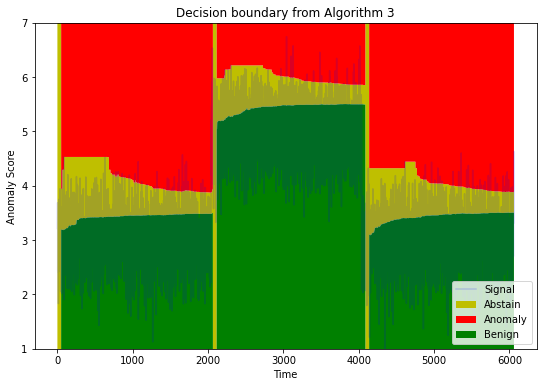
\includegraphics[width=\linewidth]{anomaly/figs/4-2.png}
  %\caption{A subfigure}
  \caption{}
  \label{fig:s41}
\end{subfigure}%
\begin{subfigure}{.48\columnwidth}
  \centering
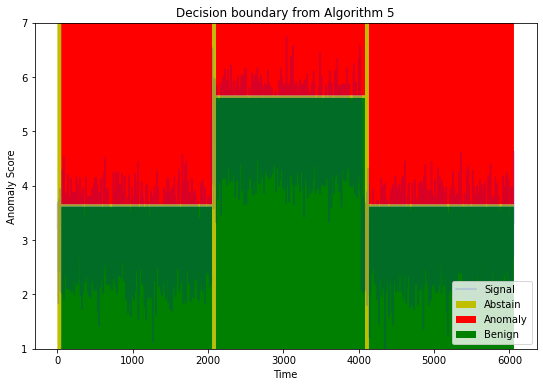
\includegraphics[width=\linewidth]{anomaly/figs/4-1.png}
  %\caption{Anomaly threshold set using a fixed cold-start period}
  \caption{}
  \label{fig:s42}
\end{subfigure}%
\vspace{-0.5em}
\caption{Decision boundaries for the same synthetic data stream, without offline dataset $(a)$ and with $(b)$. Incorporating datasets allows us to significantly reduce abstention.}\vspace{-2em}
\label{fig:s4_example}
\end{figure}
%\vspace{-4em}

%\textbf{Mistakes do not scale with $T$.}
   
% \begin{itemize}
%     \item Case $\Delta = 0$:
%     \begin{itemize}
%         \item $FP= 0$, $FN=0$
%         \item Abstains $= 4 \sqrt{(N+T) \ln \left( \frac{1612\ln(e(N+T))}{\alpha^2} \right)}- 4 \sqrt{N \ln \left( \frac{1612\ln(eN)}{\alpha^2} \right)}$
%     \end{itemize}
%     \item Case  $\Delta > 0$:
%     \begin{itemize}
%         \item $FP+FN \leq D(\Delta,\alpha) $
%         \item Abstains $\leq D(\Delta,\alpha) + 4 \sqrt{T \ln \left( \frac{1612\ln(eT)}{\alpha^2} \right)}$
%     \end{itemize}
% \end{itemize}

%We show in Corollary \ref{cor:general_flex_1} that when the offline datasets when, abstains are reduced (see also Figure \ref{fig:s4_example}).

\textbf{Abstains reduced if offline data is useful.}
     Suppose the online stream $(S_t)_{t=1}^T$  and the offline datasets  $\gD_{1}, \ldots, \gD_K$ are such that for all segments $k \in [H_T]$, there exists an offline dataset $j \in [K]$ s.t. $Q^{(k)}(p) = Q_{(j)}(p)$. Theorem \ref{thm:core_theorem} guarantees that  abstains $\leq \mathcal{O}\left(\sqrt{H_T N} \left(\sqrt{1+\frac{T}{N}} - 1 \right)\right) + \sum_{k=1}^{H_T}\widetilde{D}_k( \alpha)$, where $N = \min \{N_j \text{ : } \exists k \in [H_T] \text{ : } Q_{(j)}(p) = Q^{(k)}(p) \}  $ is size of the smallest useful offline dataset. Thus, if the useful offline data is large ($N >> T$), the fraction of abstains is small even in the presence of non-stationarity (Fig. \ref{fig:s4_example} ). 
     %\label{cor:general_flex_1}
     
%Corollary \ref{cor:general_flex_1} shows that in the worst-case when the offline distribution can be arbitrary, the performance degradation is bounded. 

\textbf{Bounded degradation if offline data is arbitrary.}
Theorem \ref{thm:core_theorem} proves that in the worst-case when the offline datasets are arbitrary, abstains are at-most $ \mathcal{O}(\sqrt{H_T T}) + \sum_{k=1}^{H_T}\widetilde{D}_k(\alpha)$, which is comparable to Theorem \ref{thm:online_shift}, with an additional additive term of $\sum_{k=1}^{H_T}\widetilde{D}_k(\alpha)$. This extra term arises due to incurring delay in both identifying a change-point on the online stream, and deciding that either the new segment has the same $p$th quantile as one of the offline datasets or not. This penalty is incurred since Algorithm \ref{alg:five} does not know both the time of change-points and if the $p$th quantile of any offline datasets equals that of the online. Thus, Theorem \ref{thm:core_theorem} is adaptive, yielding low mistakes and abstains in the event that the offline dataset is useful while simultaneously bounding worst-case performance independent of $T$ and $N$ when the offline dataset is arbitrary. 


     %For a desired $\alpha \in (0,1)$, suppose the online stream $(S_t)_{t=1}^T$ satisfy the conditions in Theorem \ref{thm:core_theorem}  and the offline datasets  $\gD_{1}, \ldots, \gD_K$ satisfy Assumption \ref{as:offline_detectable}, but are otherwise arbitrary. Then, with probability at-least $1- (K+T)\alpha$, 
     %\label{cor:general_flex_2}

%Corollary \ref{cor:general_flex_2} shows that in the worst case when the offline distributions are arbitrary, the number of abstains  %Moreover, the worst case bound is independent of stream length $T$ and offline dataset size $N$. 

% \begin{remark}[Best case scenario for Algorithm \ref{alg:five}] Even though the worst case bounds of Theorem \ref{thm:core_theorem} is the same as that of Theorem \ref{thm:online_shift} (online distribution shift setting), we can apply the analysis of Theorem \ref{thm:setting_3} (stationary + dataset setting) on each stationary piece of the stream. If all of the pieces match the offline datasets, the number of abstains is reduced to be less than $ \sum_{k=1}^{H_t} \left( D(\Delta_k,\alpha) + \gO(\sqrt{N+(\tau_k-\tau_{k-1})} - \sqrt{N})\right) $. 
% \end{remark}




%\abishek{Add flex of how this result is proved.}



\section{Experiments}
%\vspace{-0.8em}
\subsection{Synthetic data experiments}
%\vspace{-0.8em}
We evaluated our algorithm using two synthetic datasets, reflecting all scenarios discussed in this paper. The metrics are abstention percentages (Abs. \%) and mistake counts (FP + FN), averaged over 1000 streams each with 2000 samples drawn from Normal distributions with random parameters, with $p=1-10^{-2}$ and $\alpha=10^{-3}$. Our comparisons against common thresholding baselines: $\tau^{30\%}$ for static thresholding, {\ttfamily DSpot} for dynamic thresholding, and {\ttfamily EQ} for empirical quantiles using online gradient descent, are presented in Table \ref{tab:synthetic}. Implementation details and additional experiments on Pareto distributions are in Appendix \ref{app:exp1}. These results confirm our algorithm's high accuracy, adaptability to distribution shifts, and effective learning from offline data, as outlined in Section 1's desiderata. Figure \ref{fig:synthetic} illustrates how our algorithm's abstention rates and errors grow over time, corroborating our theoretical results.
%theory that (1) our algorithm makes very little FP and FN, and (2) abstains are reduced significantly with the introduction of offline datasets.  evident in the low number of mistakes,
\begin{table}[h!]
    \centering
    \begin{tabular}{cc|c|c |c| c|c}
    \toprule
        shift & data &  & Ours &  $\tau^{30\%}$  & DSpot & EQ \\
        \midrule
        \midrule
         \multirow{2}{*}{x}  & \multirow{2}{*}{x}  &
         Abs. \%& $12.1$ \plusminus{1.4} & $30$ & $15$ & $0$ \\
          && FP+FN & $\mathbf{0}$ \plusminus{0}  & $5.3$ \plusminus{3.7} & $9.1$ \plusminus{3.6} & $3.9$ \plusminus{2.1}  \\
          \midrule
         \multirow{2}{*}{\checkmark}  & \multirow{2}{*}{x}  &  
         Abs. \%& $32.7$ \plusminus{9.1} & $30$ &  $15$ & $0$  \\
        && FP+FN & $\mathbf{5.2}$ \plusminus{1.3} &  $195$  \plusminus{71} & 225 \plusminus{95} & 219 \plusminus{71} \\
                    \midrule
        \multirow{2}{*}{x} & \multirow{2}{*}{\checkmark}  &  
        Abs. \% & 9.3 \plusminus{1.2} & $30$&  $15$ & $0$ \\
          && FP+FN  & $\mathbf{0}$ \plusminus{0} & $5.3$ \plusminus{3.7} & $9.1$ \plusminus{3.6} & $3.9$ \plusminus{2.1} \\
                    \midrule
        \multirow{2}{*}{\checkmark} & \multirow{2}{*}{\checkmark}  &  Abs. \% & $18.9$ \plusminus{4.1} &$30$ &  $15$ & $0$ \\
          && FP+FN & $\mathbf{2.0}$ \plusminus{1.5}  & 155 \plusminus{69} & 173 \plusminus{64} & 160 \plusminus{64} \\
         \bottomrule
    \end{tabular}
    \caption{Synthetic dataset results. We used Algorithm 1, 3, 4, 5 as ``ours" for the four settings respectively. Compared to baselines, we achieve significant less mistakes (FP+FN) with low abstain rate, especially in settings with shift.}
    \label{tab:synthetic}
\end{table}


\begin{figure}
\centering
% \begin{subfigure}{.45\columnwidth}
%   \centering
%   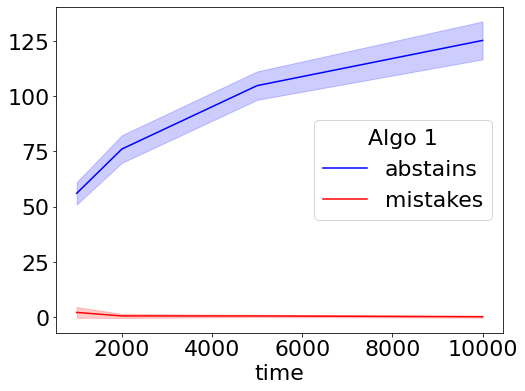
\includegraphics[width=\linewidth]{anomaly/figs/growth.png}
%   %\caption{Anomaly threshold set using a fixed cold-start period}
%   %\caption{}
%   %\label{fig:synthetic1}
% \end{subfigure}%
% \begin{subfigure}{.45\columnwidth}
%   \centering
%   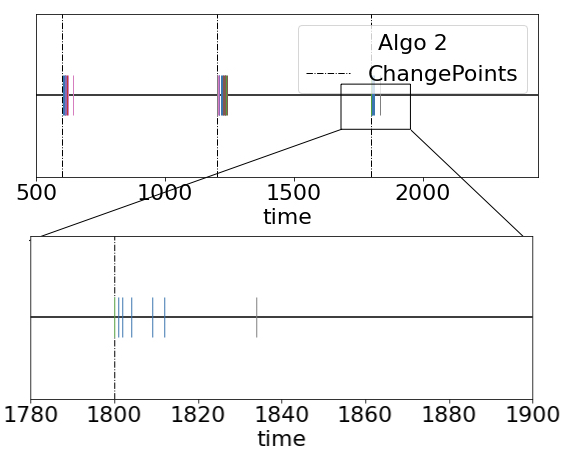
\includegraphics[width=\linewidth]{anomaly/figs/mistakes.jpeg}
%   %\caption{A subfigure}
%   %\caption{}
%   %\label{fig:synthetic2}
% \end{subfigure}
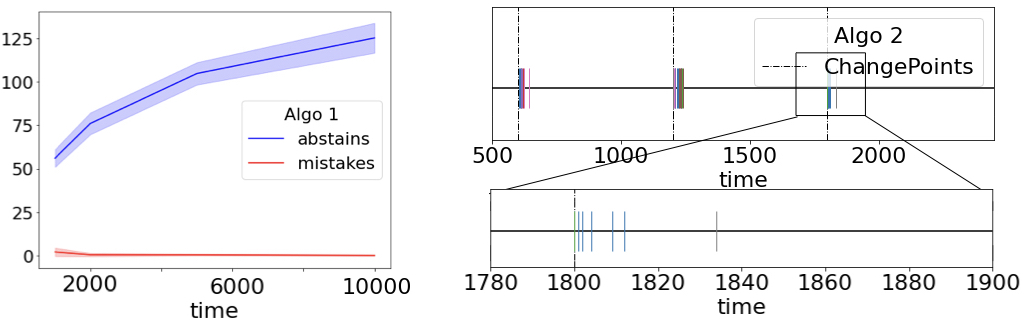
\includegraphics[width=0.95\linewidth]{anomaly/figs/exp1.jpeg}
\caption{\textit{Left:} algorithm 1, Abstains grows at $\gO(\sqrt{T})$. \textit{Right:}  algorithm 2, timestamp of mistakes in 10 random streams with aligned change points. Mistakes cluster right after change points, only as detection delay.}
\label{fig:synthetic}
\end{figure}

\subsection{MNIST anomaly detection}

We tested our algorithms on the MNIST dataset for one-class anomaly detection to demonstrate their real-world efficacy. We designated even digits as normal and odd digits as anomalous, and created data streams by sampling (e.g. Fig \ref{fig:mnist}). To show synergy of our thresholding algorithm with standard anomaly detection algorithms, we obtain anomaly scores from two models: convolutional autoencoder neural networks (NN) and isolation forests (IF), both trained on the normal class. With parameters set at $p = 0.99$ and $\alpha = 0.01$ for streams of 1000 samples, Table \ref{tab:mnist} illustrates our algorithm's improved performance over baselines.

\begin{table}[]
    \centering
    \begin{tabular}{l|c c||l | c c}
    \toprule
       Static  & abstains &  FP+FN  & Shift & abstains & FP+FN  \\
    \midrule
    $\tau^{30\%}$ & 327 \plusminus{0} & 12.7 \plusminus{0.9} &  $\tau^{30\%}$ & 670 \plusminus{0} & 91 \plusminus{8.0}\\
    DSpot & 150 \plusminus{0} & 78.1 \plusminus{2.5}  & DSpot & 150 \plusminus{0} & 129.5 \plusminus{10.2} \\
    IF+A1 & 172 \plusminus{16} & 17.6 \plusminus{5.3}  & IF+A3 & 190  \plusminus{39} & 75.7 \plusminus{18.9}\\
    NN+A1 & 133 \plusminus{4} & \textbf{3.9} \plusminus{0.7}  & NN+A3 & 339 \plusminus{12} & \textbf{9.3} \plusminus{2.1} \\
    NN+A5 & 89 \plusminus{6} & \textbf{2.1} \plusminus{0.2}  &  NN+A5 & 210 \plusminus{8} & \textbf{8.8} \plusminus{2.3} \\
    \bottomrule
    \end{tabular}
    \caption{One class MNIST result. We applied our algorithms (A as shorthand) to anomaly scores generated by Isolation Forest (IF) and neural networks (NN) and achieve much lower mistakes with moderate number of abstains. }
    \label{tab:mnist}
\end{table}

\begin{figure}
    \centering
    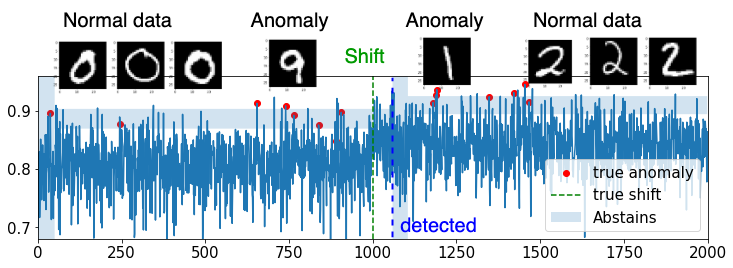
\includegraphics[width=0.9\linewidth]{anomaly/figs/Diagram2.png}
    \caption{MNIST experiment setup and a sample stream of (NN+A5) result. We choose a different set of digits for normal and anomaly to create the distribution shift, which our algorithm detects with a small delay. }
    \label{fig:mnist}
\end{figure}

\subsection{Case study of real AD application}

We also perform a case study on two real world datasets ({\ttfamily DS1} and {\ttfamily DS2}) obtained from large scale cloud computing services. Each dataset is a stream of anomaly scores obtained by applying the same black box anomaly detection algorithm (Details in Table \ref{tab:real_data_stats}). The practically motivated target in these datasets is to report $0.001\%$ anomalies, i.e., $p = 1-10^{-6}$.
Table \ref{tab:real_data} in the appendix reports the full result and comparison to baselines. We found that {\em(i)} our method achieves desired anomaly volume, {\em(ii)} incorporating offline data reduces the number of abstains without changing the volume of anomalies raised, and {\em(iii)} the volume of anomalies detected by all other methods are an order of magnitude higher leading to alert-fatigue. 


\section{Related Work}
\vspace{-0.2em}
\textbf{Dynamic thresholding for AD.} AD is an extensively researched topic, where a common paradigm is to first model data likelihood and then use a threshold to decide if a data point is normal or anomalous. This threshold is typically determined by an expert or offline through cross-validation \cite{luo2021deep, schmidl2022anomaly}. Dynamic and automatic methods makes AD algorithms more practical in real-world deployment \cite{ali2013automated, hundman2018detecting}, and are necessary where the data distribution can shift \cite{siffer2017anomaly}.  Our work is the first to provide abstain and mistake bounds on dynamic thresholding without assumptions on the underlying data distribution. Appendix \ref{app:related} contains more related work. %Using learned threshold to make binary decision of seeking labels from human experts are studied in active learning \cite{balcan2007margin, zhang2016online,vishwakarma2023promises}. However, active learning does not have a concept of mistakes and is thus different from ours. 

%\cite{siffer2017anomaly, , hundman2018detecting}
%This work instead focuses on providing a principled analysis of the thresholding step that follows. Traditionally, and are chosen by heuristics . Works closer to us are thresholding algorithms for univariate online streams .
%\vspace{-0.5em}
\textbf{Confidence Sequences (CS).} We incorporate theoretical results of confidence sequences \cite{ramdas2022game} in our analysis. \cite{maharaj2023anytime, howard2022sequential} derived the CS algorithm for estimating quantiles online with any-time guarantees, and \cite{shekhar2023sequential} leverages CS for detecting distribution shifts. 
\vspace{-0.5em}


\section{Discussion}

Our paper is the first to systematically theoretically and empirically show that thresholding algorithm can improve the overall performance of any anomaly scoring model for online anomaly detection. Through a simple argument (Theorem \ref{thm:main_lower_bound}), we demonstrate that abstaining is necessary for high accuracy. 

Our work introduces a new approach to online adaptive anomaly thresholding, leveraging CS to utilize offline data and dynamically adjust thresholds in real-time data streams. We give the first statistical guarantees on abstains and mistakes in various settings with non-stationary data streams and offline datasets (Theorem 2 - 6), motivated by practical AD applications. Our results are corroborated with synthetic and real experiments. %Future work can involve giving guarantees on threshold selection when the anomaly scores evolve through auto-regressive or temporal dependence. Another direction of future work is to relax Assumptions \ref{asumption_detectable} and \ref{defn:offline_datasets}.
%A limitation is that our results rely on assumptions of (1) samples are temporally independent and (2) change points are far apart and changes are detectable. Future work can involve giving guarantees on threshold selection when the anomaly scores evolve through auto-regressive or temporal dependence. 

A limitation of our work is that the theoretical results rely on (1) samples are temporally independent and (2) change points are far apart and changes are detectable. These assumptions, although standard in theoretical literature, need not necessarily hold in all applications.
Our algorithms also do not apply to cases when scores are temporal dependent, or if there are gradual drifts in the score distribution. Designing algorithms that provably work for these cases likely requires new techniques and is thus left for future work.

%Our insight is to use confidence sequences (CS) as both adaptive cold-start, as well as to test for distribution changes. Further, CS also enabled us to prove improved performance in the presence of offline datasets. 

%We address some possible questions and criticisms to our work. Our work abstracts away the modeling portion of anomaly detection, and instead focus on the decision making part. In this paper, we propose a new approach to thresholding; hence we consider challenges such as time-window, types of anomaly as beyond our scope. For estimating the quantiles, this work extensively uses \cite{howard2022sequential}'s confidence sequence method; their analysis focuses on estimation.  Our contribution lies in the algorithms and analyses of decision making regret given these estimations. Our algorithm is invariant to scale, offset, and occlusion. We are able to prove that algorithms fulfill the desiderata of AD outlined in section 1.2, and shown their effectiveness on large synthetic and real world datasets.

%Our setting, though uncommon in the anomaly detection literature, is motivated by practical use cases. In large cloud database/software systems, we often have a ``quota''  of anomaly alarms that we are allowed to send. How to decide which event to alarm while minimizing harmful events such as false positives and negatives becomes the research topic. As we have shown, our setting is neither simplistic or trivial \cite{wu2021current}, and our method achieve performance consistent with our theory on real datasets.



%%%%%%%%%%%%%%%%%%%%%%%%%%%%%%%%%%%%%%%%%%%%%%%%%%%%%%%%%%%%
%\clearpage



% \section{Corrections to the main paper}
% \begin{itemize}
%     \item Assumption \ref{asumption_detectable} has a mistake. We replaced the maximum $\max(D(\Delta_{k-1},\alpha), D(\Delta_{k},\alpha))$, by addition $D(\Delta_{k-1},\alpha) + D(\Delta_{k},\alpha)$.
%     \item Additional offline detectability assumption is needed in Section 5 and 6. We introduce them in the proofs as assumption \ref{as:offline_detectable} . See appendix F for details.
%     \item In Table 2, the column name ``Algo 4" should be ``Algo 3", the general algorithm. 
% \end{itemize}
% \vfill
\section{Illustrations}

We give schematic of the various settings and special cases studied in this paper. 

\begin{figure}[h!]
\centering
\begin{subfigure}{.45\columnwidth}
  \centering
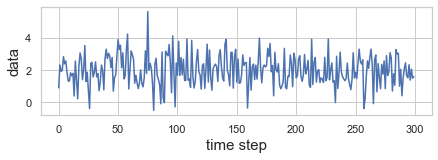
\includegraphics[width=\linewidth]{anomaly/figs/s1.png}
  \caption{Special Case I: stationary stream}
  \label{fig:s71}
\end{subfigure}%
\begin{subfigure}{.45\columnwidth}
  \centering
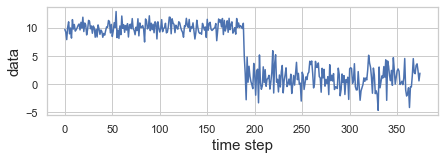
\includegraphics[width=\linewidth]{anomaly/figs/s2.png}
  \caption{Special Case II: distribution shift }
  \label{fig:s72}
\end{subfigure} \\
\begin{subfigure}{.45\columnwidth}
  \centering
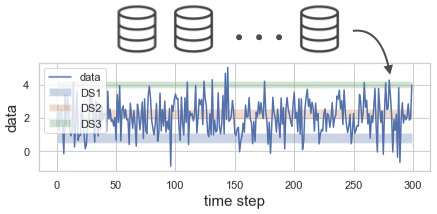
\includegraphics[width=\linewidth]{anomaly/figs/s3.jpeg}
  \caption{Special Case III: offline dataset }
\end{subfigure}%
\begin{subfigure}{.45\columnwidth}
  \centering
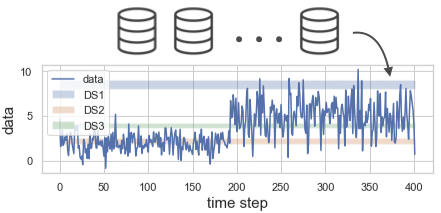
\includegraphics[width=\linewidth]{anomaly/figs/s4.jpeg}
  \caption{The General Case}
\end{subfigure}%
\caption{Illustration of the cases we study in this paper.}
\label{fig:setting_illustrations}
\end{figure}


\begin{figure}[h!]
    \centering
    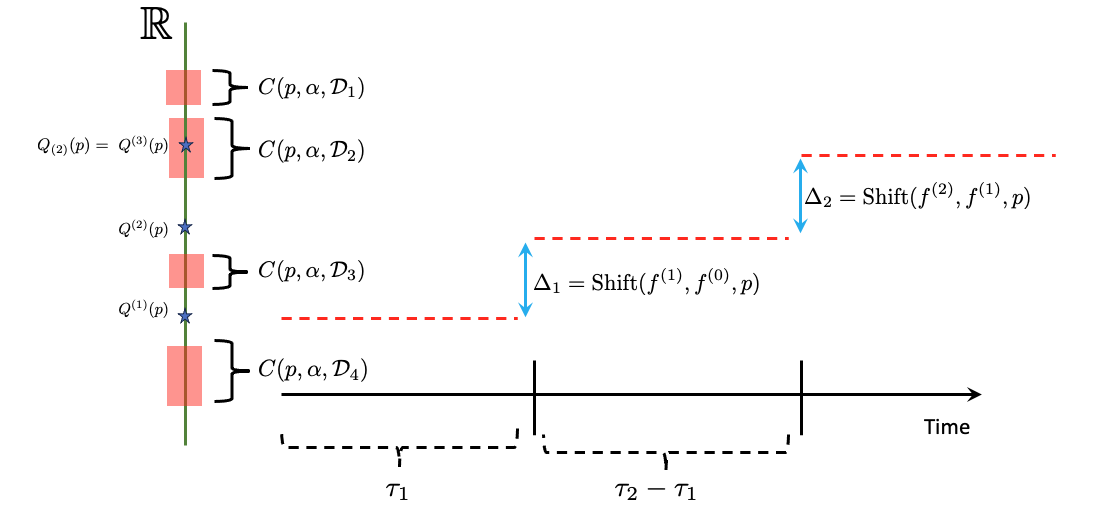
\includegraphics[width=0.8\linewidth]{anomaly/figs/separated_datasets.png}
    \caption{An illustration of Assumption \ref{asumption_detectable} and \ref{defn:offline_datasets} on a stream with $2$ change-points ($H_T=2)$ and $K=4$ offline datasets. Assumption \ref{asumption_detectable} implies that the change-points on the stream are sufficiently far apart. Assumption \ref{defn:offline_datasets} implies that the $4$ CS do not intersect. Moreover, either the true quantile on the stream are outside the offline CS, i.e., $Q^{(1)}(p)$ and $Q^{(2)}(p)$ are not contained in any offline dataset's CS. Or, it is the case that the online quantile matches one of the offline dataset, i.e., $Q_{(2)}(p) = Q^{(3)}(p)$ in this example.}
    \label{fig:separated_datasets_example}
\end{figure}

\pagebreak

\section{Proof of Theorem \ref{the:iid}, stationary setting}

\begin{algorithm}
\caption{OAD for stationary i.i.d. stream}\label{alg:one}
\SetKwInOut{Input}{Input}
\SetKwInOut{Output}{Output}
\Input{Quantile $p$, Confidence $1-\alpha$}
\Output{Anomaly labels $\hat{y}_1, \hat{y}_2, \ldots$}
\For{  $\text{each time }t \geq 1$ } {
    Receive $t^{th}$ input $S_t$\;
    
    Compute $C(p,\alpha, S_{1:t})$ (Eq. \ref{eq:cs})\;

    $\hat{y}_t \gets \text{{\ttfamily Algorithm }\ref{alg:marginal_decision}}(S_t, C(p,\alpha, S_{1:t}))$ \;
    
  %   %Compute $ub_t \gets \hat{Q}_t(p + u_t)$(Eq. \ref{eq:cs})\; 
  %   \uIf{$S_t > \max C(p,\alpha, S_{1:t})$}{
  %   $\hat{y}_t \gets1$\; \tcp{Declare an anomaly}
  % }
  % \uElseIf{$S_t \in C(p,\alpha , S_{1:t}$}{
  % $\hat{y}_t \gets * $ \; \tcp{Abstain from decision}
  % }
  % \Else{
  %   $\hat{y}_t \gets 0 $ \; \tcp{Declare benign}
  % }
}
\end{algorithm}

\begin{theorem}[Formal version of Theorem \ref{the:iid}]
If the data-source $S_1, S_2, \cdots$ are i.i.d., then with probability at-least $1-2\alpha$, for all times $T \in \mathbb{N}$, Algorithm \ref{alg:one} satisfies \begin{enumerate}
    \item $0$ False positives, $0$ False negatives
    \item Abstains is less than or equal to $7 \sqrt{T \ln \left( \frac{1612\ln(eT)}{\alpha^2} \right)}$,
    \item Abstains is at-least $\frac{1}{4} \sqrt{T \ln \left( \frac{1612\ln(eT)}{\alpha^2} \right)}$
    
\end{enumerate}
\label{the:iid_plus}
\end{theorem}
 
\begin{proof}
In order to give the proof, we set some notations. 

%
\begin{definition}[Good event $\gE_1$] %Denote the good event $\mathcal{E}_1$ as 
\begin{align}
\begin{split}
    \mathcal{E}_1 := \bigcap_{t \in \mathbb{N}} \bigcap_{p \in (0,1)} 
 \{  \widehat{Q}(p-u_t(\alpha), S_{1:t}) \leq Q(p) \leq \widehat{Q}(p+u_t(\alpha), S_{1:t}) \} .
\end{split}
\label{eqn:good_event_defn}
\end{align}   
\end{definition}
\vspace{-0.5em}
%
In words, the good event states that for all time $t$, the confidence sequence contains the true $p$th quantile.
From Corollary $2$ of \cite{howard2022sequential}, we know that $\mathbb{P}[\mathcal{E}] \geq 1-\alpha$. We remark that \cite{howard2022sequential} show that even when $(S_t)_{t \geq 1}$ are independent, but not necessarily identical, $\mathbb{P}[\mathcal{E}] \geq 1-\alpha$ holds as long as the $p$th quantile $Q_t(p) := Q(p)$ for all $t \geq 1$. This extension relaxing the identical distribution will be crucial in the subsequent sections in the sequel. 

Further, observe from the definition in Algorithm \ref{alg:one} and Equation (\ref{eq:cs}) that for all $t\in \mathbb{N}$ and $p \in (0,1)$,
\begin{align*}
     \{  \widehat{Q}(p-u_t(\alpha), S_{1:t}) \leq Q(p) \leq \widehat{Q}(p+u_t(\alpha), S_{1:t}) \} \subseteq \{ Q(p) \in C(p,\alpha, S_{1:t} \}.
\end{align*}

The reason for this inclusion is that the definition of $C(\cdot)$ in Equation (\ref{eq:cs}) has an extra factor of $2$, i.e., 
\begin{align*}
    C(p,\alpha,S_{1:t}) :=  \bigg[ \widehat{Q}(p- 2u_{n}(\alpha), y_{1:n}),  \widehat{Q}(p+2u_{n}(\alpha), y_{1:n}) \bigg].
\end{align*}


% Recall the good event $\mathcal{E}$ as defined in equation \ref{eqn:good_event_defn}.
% \begin{align*}
%     \mathcal{E} := \bigcap_{t \in \mathbb{N}} \bigcap_{p \in (0,1)} \{ Q(p) \leq \widehat{Q}_t(p+u_t) \} \bigcap \{ Q(p) \geq \widehat{Q}_t(p-u_t) \}.
% \end{align*}
% From Corollary $2$ of \cite{howard2022sequential}, we know that $\mathbb{P}[\mathcal{E}] \geq 1-\alpha$. 

In the rest of this proof, we will assume that the good event $\mathcal{E}$ holds. It is immediately clear the following two claims hold, proving the first two statements of the theorem.
\begin{claim}
If event $\mathcal{E}$ holds, then Algorithm 1 will not make any False Positive or False negative detections.
\label{claim:goodevent1}
\end{claim}

It now only remains to prove the third condition of the theorem. Define the sequence of indicator random variables indicating if time $t$ is an abstain
\begin{align} 
    Z_t := \mathbf{1}(\widehat{y}_t = *) .
\end{align} 

From Algorithm \ref{alg:one}, this is equivalent to 
\begin{align*}
    Z_{t} = \mathbf{1}(S_{t} \in (\widehat{Q}_t(p-2u_{t-1}(\alpha), S_{1:t-1}), \widehat{Q}_t(p+2u_{t-1}(\alpha), S_{1:t-1})).
\end{align*}
We denote by the filtration $(\mathcal{F}_t)_{t=1}^T$ to be generated by the observed sequence $(S_t)_{t=1}^T$, i.e., for all $t \in \{1,\cdots,T\}$, $\mathcal{F}_t := \sigma(S_1,\cdots,S_t)$. 


The proof of claim \ref{claim:goodevent1} follows from the following three lemmas. For clarity, proof for these lemmas can be found after this proof finishes.
 
% \begin{lemma}[Expectation of abstains] For every $t\geq2$, we have $\E(Z_t) \leq 3u_{t-1}(\alpha)$.
% \label{lem:exp_z}
% \end{lemma}

\begin{lemma}[Conditional expectation of abstains]
For every $ t \geq 2$, $$4u_{t-1}(\alpha) \leq \E[Z_t \mathbf{1}_{\mathcal{E}}| \mathcal{F}_{t-1}] \leq 6u_{t-1}(\alpha),$$ holds almost-surely.  
\label{lem:cond_exp}
\end{lemma}

\begin{lemma}[Azuma-Hoefding bound] 
Let $(Z_t)_{t=1}^T$ are bounded binomial variables and the sequence $(\mathcal{F}_t)_{t=1}^T$ is a probability filtration. Then for all $\varepsilon > 0$,
\begin{align*}
    \mathbb{P} \left[ \bigg| \sum_{s=1}^T Z_s  - \mathbb{E}[Z_s  \vert \mathcal{F}_{s-1}] \bigg| \geq \varepsilon \right] \leq 2 \exp \left( -\frac{ \varepsilon^2}{2T} \right)
\end{align*}
\label{lemma:azuma}
\end{lemma}

We now apply Lemma \ref{lemma:azuma} to the sequence of binary random variables $(\widetilde{Z}_t)_{t\geq 1} := (Z_t \mathbf{1}_{\mathcal{E}})_{t \geq 1}$ by setting $\varepsilon =  \sqrt{T \ln \left( \frac{4}{\alpha^2} \right)}$. Thus, with probability at least $1-\alpha$ %? $1-\frac{\alpha}{2}$
, we have

\begin{align*}
  \mathbb{P} \left[ \underbrace{ \bigg| \mathbf{1}_{\mathcal{E}} \sum_{s=1}^TZ_s - \sum_{s=1}^T \mathbb{E}[Z_s \mathbf{1}_{\mathcal{E}} \vert \mathcal{F}_{s-1}] \bigg| \leq   \sqrt{T \ln \left( \frac{4}{\alpha^2} \right)}}_{\text{Event } \mathcal{G}_1} \right] \geq 1- \alpha
  \end{align*}
  
From a simple union-bound argument, we see that $\mathbb{P}[\mathcal{E} \cap \mathcal{G}_1] \geq 1 - 2\alpha$. Furthermore by definition of event $\mathcal{G}_1$,  the following inequality holds almost-surely. 
\begin{align*}
    \mathbf{1}_{\mathcal{G}}\mathbf{1}_{\mathcal{E}_1} \sum_{s=1}^TZ_s &\leq \mathbf{1}_{\mathcal{G}_1}\left(\sum_{s=1}^T \mathbb{E}[Z_s \mathbf{1}_{\mathcal{E}} \vert \mathcal{F}_{s-1}] +  \sqrt{T \ln \left( \frac{4}{\alpha^2} \right)}\right),\\
        &\stackrel{\text{Lem } \ref{lem:cond_exp}}{\leq}  \mathbf{1}_{\mathcal{G}_1}\left( \sum_{t=1}^T 6u_{t-1}(\alpha) + \sqrt{T \ln \left( \frac{4}{\alpha^2} \right)}\right), \\
    &\stackrel{}{\leq}  \mathbf{1}_{\mathcal{G}_1}\left(6\sqrt{T \ln \left( \frac{1612 \ln(eT)}{\alpha} \right)} + \sqrt{T \ln \left( \frac{4}{\alpha^2} \right)}\right), \\
   &\leq  \mathbf{1}_{\mathcal{G}_1}\left(7\sqrt{T \ln \left( \frac{1612 \ln(eT)}{\alpha^2} \right)}\right).
\end{align*}
In other words, the preceding display reads that on the event $\mathcal{E} \cap \mathcal{G}_1$ holds, we have
  \begin{align*}
   \sum_{s=1}^TZ_s \leq 7\sqrt{T \ln \left( \frac{1612 \ln(eT)}{\alpha^2} \right)}.
\end{align*}
Similarly, from the definition of $\mathcal{G}_1$, we also have 
\begin{align*}
     \mathbf{1}_{\mathcal{G}}\mathbf{1}_{\mathcal{E}_1} \sum_{s=1}^TZ_s &\geq \mathbf{1}_{\mathcal{G}_1}\left(\sum_{s=1}^T \mathbb{E}[Z_s \mathbf{1}_{\mathcal{E}} \vert \mathcal{F}_{s-1}] -  \sqrt{T \ln \left( \frac{4}{\alpha^2} \right)}\right),\\
             &\stackrel{\text{Lem } \ref{lem:cond_exp}}{\geq}  \mathbf{1}_{\mathcal{G}_1}\left( \sum_{t=1}^T 2u_{t-1}(\alpha) - \sqrt{T \ln \left( \frac{4}{\alpha^2} \right)}\right), \\
    &\stackrel{}{\geq}  \mathbf{1}_{\mathcal{G}_1}\left(2\sqrt{T \ln \left( \frac{1612 \ln(eT)}{\alpha} \right)} - \sqrt{T \ln \left( \frac{4}{\alpha^2} \right)}\right), \\
   &\geq  \mathbf{1}_{\mathcal{G}_1}\left(\frac{1}{4}\sqrt{T \ln \left( \frac{1612 \ln(eT)}{\alpha^2} \right)}\right).
\end{align*}
The proof is complete since $\mathbb{P}[\mathcal{E} \cap \mathcal{G}_1] \geq 1-2\alpha$. 
\end{proof}


Below we provide the proof of each lemma used in proof of Theorem \ref{the:iid}. 

% \begin{proof}[Proof of Lemma \ref{lem:exp_z}]
% Note that again $\hat{Q}_t$ is the empirical quantile function of $\{S_i\}_{i=1}^{t-1}$. By exchangeability of i.i.d. samples, we know that the the probability of $S_t$'s rank among $\{S_i\}_{i=1}^{t-1}$ is uniform. Therefore,
% \begin{align*}
% \E(Z_t) = \prob (S_t \in [\hat{Q}(p-u_{t-1}(\alpha), S_{1:t-1}),\hat{Q}(p+u_{t-1}(\alpha),S_{1:t-1})])  \leq \frac{\ceil{2u_{t-1}(\alpha)\cdot (t-1)}}{t}  \leq  3u_t
% \end{align*}
% \end{proof}


\begin{proof}[Proof of Lemma \ref{lem:cond_exp}]
% In order to prove this result, we use the stornger Corollary $2$ of \cite{howard2022sequential}. We know from that corollary that if $g_t := 0.85\sqrt{t^{-1}(\log \log(et) + 0.8 \log (1612/\alpha))}$, then $$ \mathbb{P}[ \exists t \in \mathbb{N}, \exists p \in (0,1) : \{ Q(p) < \widehat{Q}_t(p-g_t) \} \cup  \{ Q(p) > \widehat{Q}_t(p + g_t) \} ] \leq  \alpha. $$
% Then in particular, we have
% {\color{black}
% \begin{align*}
%     \mathbb{P} \left[ \forall t, \{ Q(p+2u_t) \geq \widehat{Q}_t(p+u_t) \} \cap \text{  } \{ Q(p-2u_t) \leq \widehat{Q}_t(p-u_t) \} \right] \geq 1-\alpha. 
% \end{align*}
% }
% Thus, 
We can compute the conditional expectation as 
\begin{align*}
    \E[Z_t \mathbf{1}_{\mathcal{E}}| \mathcal{F}_{t-1}] 
    &= \mathbb{P}[S_t \in (\widehat{Q}(p-2u_{t-1}(\alpha),S_{1:t-1}), \widehat{Q}(p+2u_{t-1}(\alpha),S_{1:t-1}) ) \cap \mathcal{E} \vert \mathcal{F}_{t-1}], \\
        &\stackrel{(a)}{\leq}  \mathbb{P}[S_t \in (Q(p-3u_{t-1}(\alpha)), Q(p+3u_{t-1}(\alpha)) \vert \mathcal{F}_{t-1}]  \\
        &\stackrel{(b)}{\leq}  \mathbb{P}[S_t \in (Q(p-3u_{t-1}(\alpha)), Q(p+3u_{t-1}(\alpha)) ]  \\
    & \stackrel{(c)}{\leq} 6u_{t-1}(\alpha).
\end{align*}
Step $(a)$ follows from the fact that on event $\mathcal{E}$, for all times $t \in \mathbb{N}$ and quantiles $p \in (0,1)$, we have $Q(p) \leq \widehat{Q}(p+u_t(\alpha),S_{1:t})$ and $Q(p) \geq \widehat{Q}(p-u_t(\alpha),S_{1:t-1})$ holds. Step $(b)$ follows since $(S_t)_{t \geq 1}$ is an i.i.d. sequence and thus $S_t$ is independent of $\mathcal{F}_{t-1}$. Step $(c)$ follows from the standard fact the for any $\mathbb{R}$ valued continuous random variable, and for any quantiles $0 \leq p_1 \leq p_2 \leq 1 $, $\mathbb{P}[X \in (Q(p_1), Q(p_2))] = p_2 - p_1$.
Similarly, we have 
\begin{align*}
    \E[Z_t \mathbf{1}_{\mathcal{E}}| \mathcal{F}_{t-1}] 
    &= \mathbb{P}[S_t \in (\widehat{Q}(p-2u_{t-1}(\alpha),S_{1:t-1}), \widehat{Q}(p+2u_{t-1}(\alpha),S_{1:t-1}) ) \cap \mathcal{E} \vert \mathcal{F}_{t-1}], \\
        &\stackrel{(a)}{\geq}  \mathbb{P}[S_t \in (Q(p-u_{t-1}(\alpha)), Q(p+u_{t-1}(\alpha)) \vert \mathcal{F}_{t-1}]  \\
        &\stackrel{(b)}{\leq}  \mathbb{P}[S_t \in (Q(p-u_{t-1}(\alpha)), Q(p+u_{t-1}(\alpha)) ]  \\
    & \stackrel{(c)}{\leq} 2u_{t-1}(\alpha).
\end{align*}
follows from the fact that on event $\mathcal{E}$, for all times $t \in \mathbb{N}$ and quantiles $p \in (0,1)$, we have $Q(p) \leq \widehat{Q}(p+u_t(\alpha),S_{1:t})$ and $Q(p) \geq \widehat{Q}(p-u_t(\alpha),S_{1:t-1})$ holds. Step $(b)$ follows since $(S_t)_{t \geq 1}$ is an i.i.d. sequence and thus $S_t$ is independent of $\mathcal{F}_{t-1}$. Step $(c)$ follows from the standard fact the for any $\mathbb{R}$ valued continuous random variable, and for any quantiles $0 \leq p_1 \leq p_2 \leq 1 $, $\mathbb{P}[X \in (Q(p_1), Q(p_2))] = p_2 - p_1$.
\end{proof}

\begin{proof}[Proof of Lemma \ref{lemma:azuma}]
Denote by the sequence of $0$ mean random variables $\widetilde{Z}_t := Z_t - \mathbb{E}[Z_t \vert \mathcal{F}_{t-1}]$. Denote by the running sum $Y_t := \sum_{s=1}^{t} \widetilde{Z}_s$. It is easy to verify that $(Y_t)_{t=1}^T$ is a martingale sequence. Further from definition, we have have that almost-surely, for all $t \in \{1,\cdots, T\}$, $|Y_{t} - Y_{t+1}| \leq 2$. Thus, from Azuma Hoeffding inequality for bounded martingales, we have that 
\begin{align}
    \mathbb{P}\left[\sum_{s=1}^T \widetilde{Z}_s \geq \sqrt{T \ln \left( \frac{4}{\alpha^2} \right)}\right] &\leq 2 \exp \left( - \frac{2 T \ln \left( \frac{4}{\alpha^2} \right)}{4T} \right), \\
    &\leq \frac{\alpha}{2}.
\end{align}


\end{proof}

\section{Proofs from Section \ref{sec:offline-only}}



The proofs in this section are dependent on the following good-event, under which we will perform the analysis.

%\subsection{Good events for quantile estimation}

\begin{definition}[Good event 2] 
Let $(S_t)_{t=1}^T \sim \Bigl(T,H_T, (\tau_c)_{c=0}^{H_T}, (f^{(c)})_{c=0}^{H_T}\Bigr)$, with quantile functions of the $H_T+1$ segments given by $(Q^{(c)}(\cdot))_{c=0}^{H_T}$. Define $\gE_2$ as
\begin{align}
    \widehat{\gE_2} := \bigcap_{k=1}^{H_T} \gE_2^{(k)},
    \label{eqn:good_event_2_defn_internal}
\end{align}
where for each $k \in [H_T]$, 
\begin{align*}
        \mathcal{E}_2^{(k)} =  \bigcap_{p \in [0,1]} \bigcap_{t_1 = \tau_{k}}^{\tau_{k+1}} \bigcap_{t_2 = t_1 +1}^{\tau_{k+1}}   \bigg\{ \widehat{Q}(p-u_{t_2 - t_1}(\alpha), S_{t_1:t_2})  \leq Q^{(k)}(p) \leq \widehat{Q}(p-u_{t_2 - t_1}(\alpha), S_{t_1:t_2}) \bigg\},
\end{align*}
where $\widehat{Q}$ is the empirical quantile and $u_{(\cdot)}(\cdot)$ is defined in Equation (\ref{eqn:defn_confidence_width_ut}).
\label{as:goodevent2}
\end{definition}
%\vspace{-1em}
%
In words,  $\gE_2$ is the intersection over all the $H_T+1$ stationary segments, where for each segment the quantile estimate is close to the true quantile for all quantiles. Following Corollary $2$ of \cite{howard2022sequential} and an union bound, we get the following.

\begin{proposition}
    \begin{align*}
        \mathbb{P}[\widehat{\gE_2}] \geq 1 - T\alpha.
    \end{align*}
    \label{prop:good_event_2_prob_hat}
\end{proposition}
\begin{proof}
    We analyze the complement as follows.
    \begin{align*}
        & \quad \; \mathbb{P}[\widehat{\gE_2}^{\complement}] \\ &= \mathbb{P} \left[ \cup_{k=0}^{H_T} \cup_{p \in [0,1]} \cup_{t_1=\tau_k}^{\tau_{k+1}} \cup_{t_2 \geq t_1 + 1} \{ \widehat{Q}(p-u_{t_2 - t_1}(\alpha), S_{t_1:t_2})  > Q^{(k)}(p) \} \cup \{ Q^{(k)}(p) > \widehat{Q}(p-u_{t_2 - t_1}(\alpha), S_{t_1:t_2}) \}  \right], \\
        &\leq \sum_{k=0}^{H_T} \sum_{t_1=\tau_k}^{\tau_{k+1}}\mathbb{P} \left[ \cup_{p \in [0,1]} \cup_{t_2 \geq t_1 + 1} \{ \widehat{Q}(p-u_{t_2 - t_1}(\alpha), S_{t_1:t_2})  > Q^{(k)}(p) \} \cup \{ Q^{(k)}(p) > \widehat{Q}(p-u_{t_2 - t_1}(\alpha), S_{t_1:t_2}) \}  \right], \\
        &\stackrel{(a)}{\leq}\sum_{k=0}^{H_T} \sum_{t_1=\tau_k}^{\tau_{k+1}}\alpha, \\
        &= T \alpha.
    \end{align*}
    Step $(a)$ follows from   Corollary $2$ of \cite{howard2022sequential}.
\end{proof}

{\color{black}

In addition, we also need a generalization of event $\mathcal{G}_1$ to the piece-wise stationary stream. 

\begin{align}
  \gG_2:=  \bigcap_{k=0}^{H_T} \bigcap_{t_1 = \tau_k + 1}^{\tau_{k+1}}\bigg\{ \bigg| \sum_{t=t_1}^{\tau_{k+1}}Z_{t:t_1} - \mathbb{E}[Z_{t:t_1} \vert \mathcal{F}_{t-1}] \bigg| \leq \sqrt{(\tau_{k+1} - \tau_k) \ln \left( \frac{4}{\alpha^2} \right)} \bigg\},
  \label{eqn:good_event_G}
\end{align}
where 
\begin{align}
    Z_{t:t_1} := \mathbf{1}(S_{t} \in (\widehat{Q}_t(p-2u_{t-t_1}(\alpha), S_{t_1:t-1}), \widehat{Q}_t(p+2u_{t-t_1}(\alpha), S_{t_1:t-1})),
\end{align}
and $\mathcal{F}_{t-1} := \sigma(S_{1:t-1})$ is the sigma-algebra generated by the first $t-1$ samples.

\begin{proposition}
    \begin{align*}
        \mathbb{P}[\gG_2] \geq 1 - T \alpha.
    \end{align*}
    \label{prop:abstain_good_event}
\end{proposition}
For a given $k$ and $t_1$, the proof follows from an application of Azuma-Hoeffding similar to the proof of Theorem \ref{the:iid}. Applying an union bound over $k$ and $t_1$ yields the result. 

In the rest of this section, denote the good event $\gE_2$ as 
\begin{align}
    \gE_2 = \widehat{\gE_2} \bigcap \gG_2,
    \label{eqn:good_event_2_defn}
\end{align}
where $\widehat{\gE}_2$ is defined in Equation (\ref{eqn:good_event_2_defn_internal}) and $\gG_2$ in Equation (\ref{eqn:good_event_G}).

\begin{proposition}
    \begin{align*}
        \mathbb{P}[\widehat{\gE_2}] \geq 1 - T\alpha.
    \end{align*}
    \label{prop:good_event_2_prob}
\end{proposition}
The proof follows from an union bound using estimates in Proposition \ref{prop:good_event_2_prob_hat} and \ref{prop:abstain_good_event}.

}

\subsection{Proof of Proposition \ref{prop:delay_bound}}


\begin{figure}[h!]
    \centering
    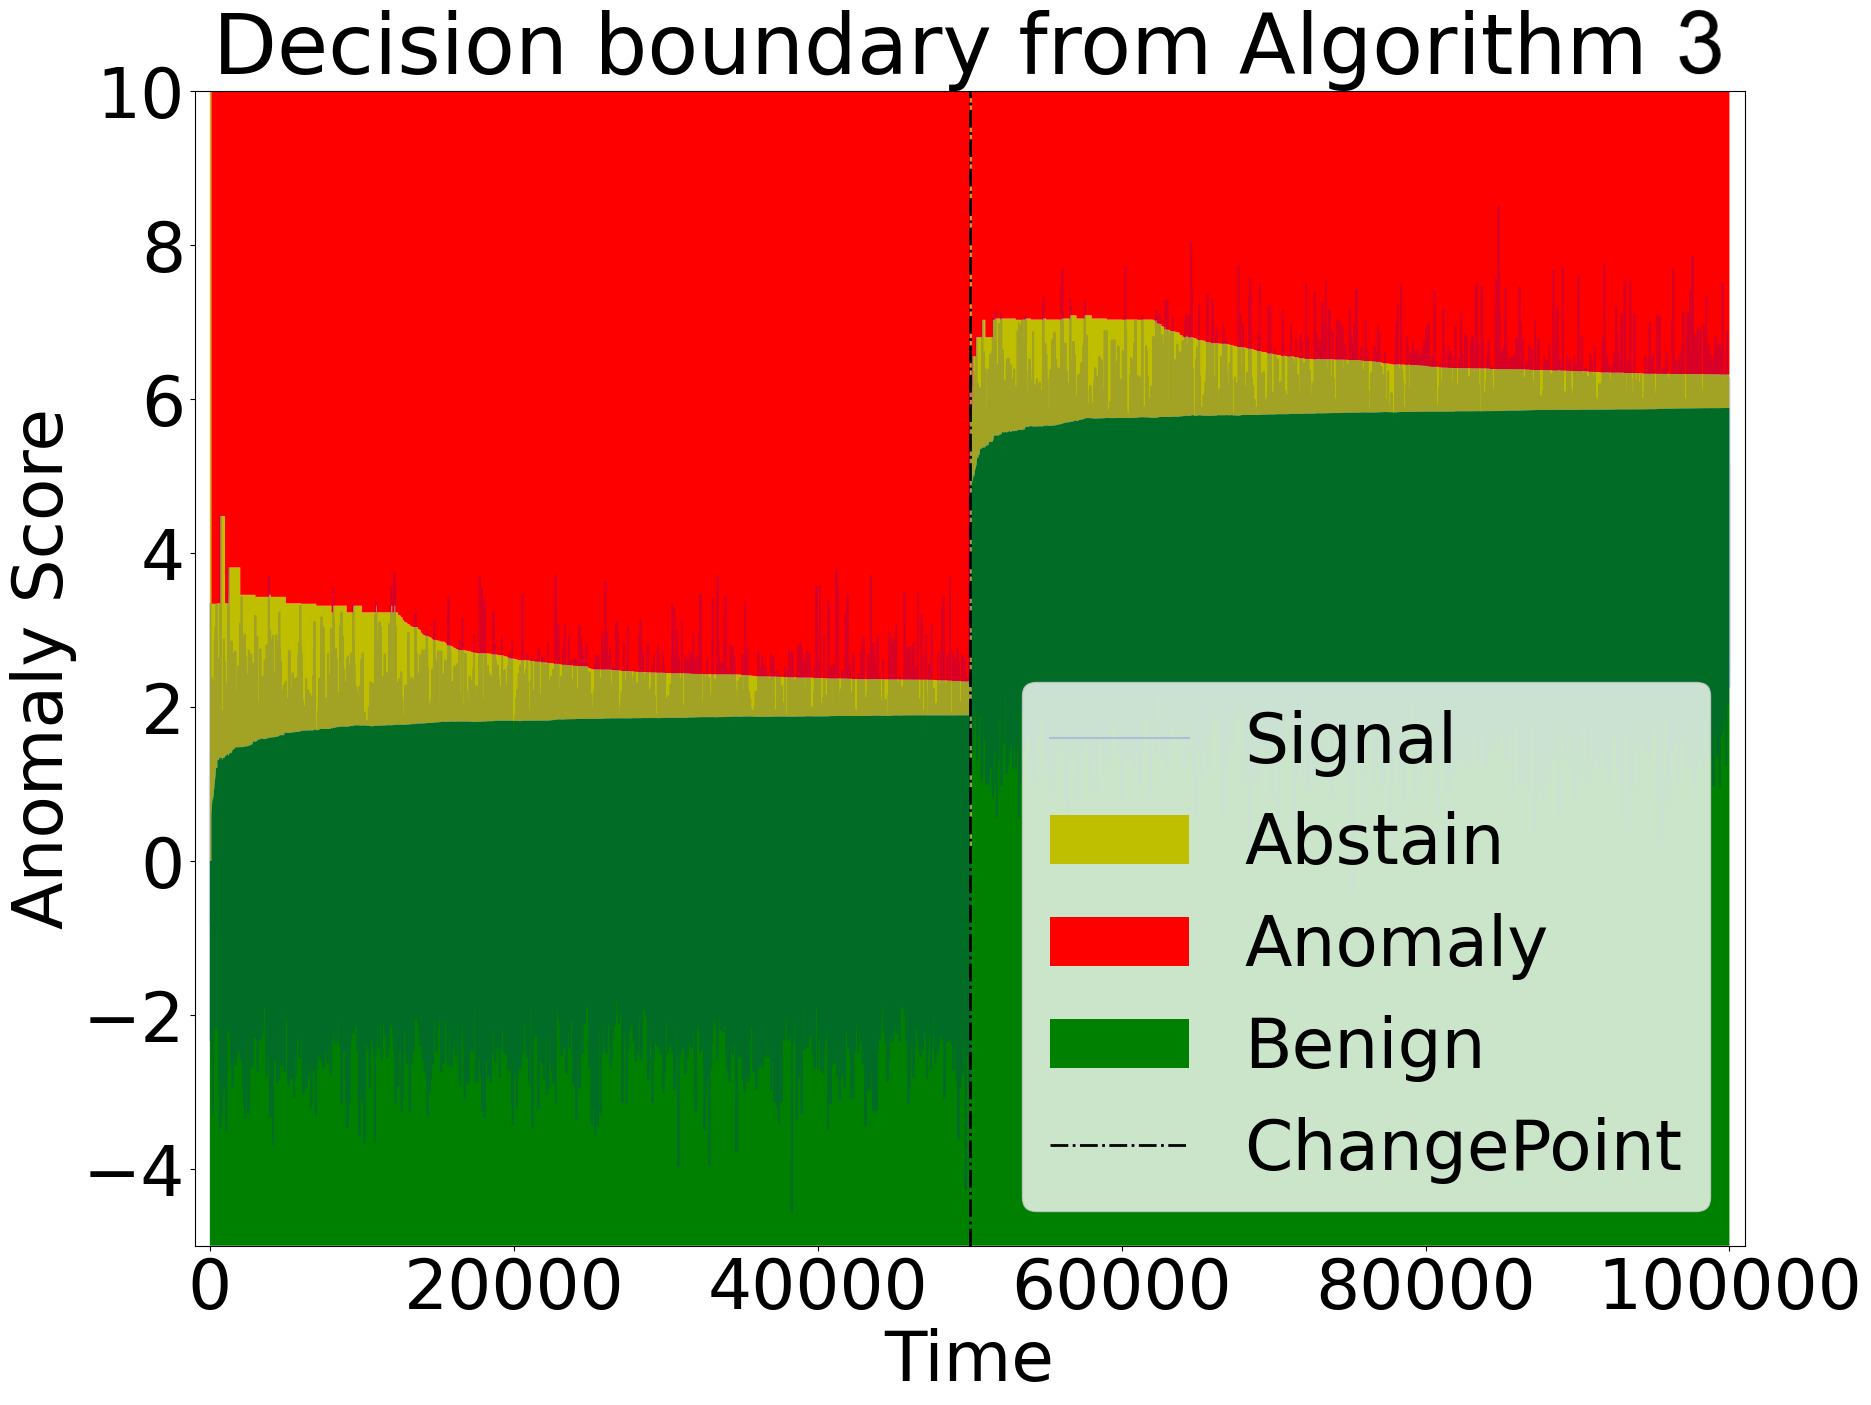
\includegraphics[width=0.4\linewidth]{anomaly/figs/algo_2_example.png}
    \caption{Algorithm 3 output on a piece-wise stationary stream.}
    \label{fig:s1}
\end{figure}

In order to give the proof of Proposition \ref{prop:delay_bound}, we need the following general lemma on change-detection. 


\begin{proposition}[Stream with a single change-point]
Let $(S_t)_{t=1}^T$ be a piecewise stationary stream with a single change-point, i.e., $H_T = 1$ with the change-point instant $\tau_1 = \tau \in [T]$. Denote by $\Delta := \text{Shift}(f^{(0)}, f^{(1)}, p)$ as the distribution shift magnitude. Denote by $\tau' \in \mathbb{N}$ as the first time when the {\ttfamily if} statement in Algorithm \ref{alg:two} evaluates to {\ttfamily True}, i.e., a change is detected for the first time by Algorithm \ref{alg:two}. Then, under the good event  $\gE_2$  (Definition \ref{as:goodevent2}), 
\begin{align*}
    \tau \leq \tau' 
    &\leq \bigg\lceil \inf_{\widetilde{\tau}} \left\{  u_{\tau}(\alpha) + u_{\widetilde{\tau}-\tau}(\alpha) \leq \frac{\Delta}{6} \right\} \bigg\rceil,
\end{align*}
where $u_t(\alpha)$ is given in Equation (\ref{eqn:defn_confidence_width_ut}). 
\label{prop:dist_changes}
\end{proposition}


We recall some notation to give the proof. The two distributions are denoted by $f^{(0)}$ and $f^{(1)}$ and their corresponding quantile functions are given by $Q^{(0)}(\cdot)$ and $Q^{(1)}(\cdot)$, where for $i \in \{0,1\}$, the function $Q^{(i)}(\cdot) : [0,1] \to \mathbb{R}$ is such that for all $p \in [0,1]$, $Q^{(i)}(p)$ is the $p$th quantile of the distribution $f^{(i)}$. Since we assume all distributions are continuous, the existence and uniqueness of quantile functions are granted. 

\textbf{Proof that $\tau \leq \tau'$}

Observe that under the event $\gE_2$, we have for all $t_1 < t_2 \in [\tau]$, $Q^{(0)}(p) \in C(p,\alpha, S_{t_1:t_2})$. Thus, for all $t \in [\tau]$, $Q^{(0)}(p) \in \bigcap_{s=1}^t C(p,\alpha,S_{s:t}) \bigcap_{s=1}^t C(p,\alpha,S_{1:s})$, and in particular, $\bigcap_{s=1}^t C(p,\alpha,S_{s:t}) \bigcap_{s=1}^t C(p,\alpha,S_{1:s})$ is non-empty. Therefore, under event $\gE_2$, for all $t \in [\tau]$, Algorithm \ref{alg:change_point} will never return {\ttfamily True} for the input sequence $S_{1:t}$.

\textbf{Proof on the upper bound of $\tau'$}

Since $\Delta > 0$, we will assume here that $Q^{(0)}(p) < Q^{(1)}(p)$ and this is without loss of generality since the proof for the other case follows identically. 
To prove the upper bound, it suffices to prove that if event $\gE_2$ holds and no change is detected till time $\tau' = \inf \{\widetilde{\tau}: u_{\tau}(\alpha)+ u_{\widetilde{\tau}-\tau}(\alpha) \}$, then at time $\lceil \tau' \rceil$, a change point will be detected. 

In order to prove this, we need to establish that $\bigcap_{s=1}^{\lceil \tau' \rceil} C(p,\alpha,S_{s:t}) \bigcap_{s=1}^{\lceil \tau' \rceil} C(p,\alpha,S_{1:s}) = \emptyset$. A sufficient condition for this is to prove that $C(p,\alpha,S_{\tau+1:\lceil \tau' \rceil}) \bigcap C(p,\alpha,S_{1:\tau}) = \emptyset$, i.e., the following implication holds 
\begin{align}
    C(p,\alpha,S_{\tau+1:\lceil \tau' \rceil}) \bigcap C(p,\alpha,S_{1:\tau}) = \emptyset \implies \bigcap_{s=1}^{\lceil \tau' \rceil} C(p,\alpha,S_{s:t}) \bigcap_{s=1}^{\lceil \tau' \rceil} C(p,\alpha,S_{1:s}) = \emptyset.
    \label{eqn:setting_2_internal_implication}
\end{align}
From Equation (\ref{eq:cs}), we know that 
\begin{align*}
     C(p,\alpha,S_{1:\tau}) = \bigg[ \widehat{Q}(p-2u_{\tau}(\alpha), S_{1:\tau}), \widehat{Q}(p+2u_{\tau}(\alpha), S_{1:\tau}) \bigg].
\end{align*}

Since event $\gE_2$ holds, it follows that 
\begin{align}
    \widehat{Q}(p+2u_{\tau}(\alpha),S_{1:\tau}) &\leq Q^{(0)}(p+3u_{\tau}(\alpha))     \label{eqn:setting_2_delay_pf_11}\\
    \widehat{Q}(p-2u_{\lceil \tau' \rceil - \tau}(\alpha)) &\geq Q^{(1)}(p - 3u_{\lceil \tau' \rceil-\tau}(\alpha)).
    \label{eqn:setting_2_delay_pf_1}
\end{align}
Further, from the definition of $\Delta$ in Definition \ref{def:quantile_shift} and the assumption that $Q^{(0)}(p) < Q^{(1)}(p)$ we know that 
\begin{align}    
Q^{(0)}( p + {\Delta} ) \leq Q^{(1)}(p - {\Delta})
    \label{eqn:setting_2_delay_pf_2}
\end{align}

Now, from the definition of $\tau'$, we know that 
\begin{align}
    3(u_{\tau}(\alpha) + u_{\lceil {\tau'} \rceil-\tau}(\alpha)) \leq {\Delta}
        \label{eqn:setting_2_delay_pf_3}
\end{align}

Now, combining the inequalities in Equations (\ref{eqn:setting_2_delay_pf_1}, \ref{eqn:setting_2_delay_pf_2}, \ref{eqn:setting_2_delay_pf_3}), we get that 
\begin{multline}
\widehat{Q}(p+2u_{\tau}(\alpha),S_{1:\tau}) \stackrel{\ref{eqn:setting_2_delay_pf_11}}{\leq} Q^{(0)}(p+3u_{\tau}(\alpha)) \stackrel{(a)}{<} Q^{(0)}(p+3u_{\tau}(\alpha) + 3u_{\lceil {\tau'} \rceil-\tau}(\alpha)) \stackrel{\ref{eqn:setting_2_delay_pf_3}}{\leq} Q^{(0)}(p+{\Delta}) \stackrel{\ref{eqn:setting_2_delay_pf_2}}{\leq} \\ Q^{(1)} ( p - {\Delta} ) \stackrel{\ref{eqn:setting_2_delay_pf_3}}{\leq} Q^{(1)}(p-3u_{\lceil {\tau'} \rceil-\tau}(\alpha)) \stackrel{\ref{eqn:setting_2_delay_pf_1}}{\leq} \widehat{Q}(p-2u_{\tau}(\alpha),S_{\tau:\lceil {\tau'} \rceil}).
\label{eqn:disjoint}
\end{multline}
Step $(a)$ follows from the fact that since $f^{(0)}$ and $f^{(1)}$ are a continuous distribution, we have for all $i \in \{0,1\}$ and a;; $0 < p_1 < p_2 < 1$, $Q^{(i)}(p_1) < Q^{(i)}(p_2)$. Thus, Equation (\ref{eqn:disjoint}) gives that under the event $\gE_2$, $   C(p,\alpha,S_{\tau+1:\lceil \tau' \rceil}) \bigcap C(p,\alpha,S_{1:\tau}) = \emptyset$, which from Equation (\ref{eqn:setting_2_internal_implication}) implies that if Algorithm \ref{alg:change_point} is queried with input $S_{1:\lceil \tau' \rceil}$, will return a {\ttfamily 1}, i.e., detect a change-point.


\textbf{Concluding the proof of Proposition \ref{prop:delay_bound} as an application of Proposition \ref{prop:dist_changes}}

% \begin{proposition*}[\ref{prop:delay_bound}]
% If the number of pre-change samples $\tau \geq \frac{20}{\Delta^2}\ln \left( \frac{1612}{\alpha \Delta^2}\right)$, then $\text{Delay}(\tau, \Delta, \alpha) \leq \frac{20}{\Delta^2}\ln \left( \frac{1612}{\alpha \Delta^2}\right).$
% \end{proposition*}

\begin{proof}
% Let $\tau$ denote the number of pre-change samples, and let $\tau'$ denote the point where the changes are detected. Delay can be defined as $\tau' - \tau$.  Suppose $\tau \geq \frac{20}{\Delta^2}\ln \left( \frac{1612}{\alpha \Delta^2}\right)$.

% For a change of magnitude $\Delta$ with $\tau$ pre-change samples to be detectable under the good event $\gE_2$, a \emph{sufficient} condition is that the forward and backward confidence sequences becomes disjoint at time $\tau$:
% \begin{align}
%     2(u_{\tau}(\alpha) + u_{\tau'- \tau}(\alpha)) \leq \Delta
% \label{eq:detectability}
% \end{align}

The proof rests on the following numerical claim.

\begin{claim}
If $\tau \geq \frac{80}{\Delta^2}\ln \left( \frac{1612}{\alpha \Delta^2}\right)$, then $u_\tau(\alpha) \leq \Delta/6 $ holds.
\label{claim:delay1}
\end{claim}
{\color{black}
\begin{proof}[Proof of Claim \ref{claim:delay1}]
Suppose $\tau \geq \frac{80}{\Delta^2}\ln \left( \frac{1612}{\alpha \Delta^2}\right)$. Then
\begin{align*} 
    u_{\tau}(\alpha) &\leq \sqrt{\frac{\ln \left( \frac{1612}{\alpha}(1+\ln(\tau)) \right)}{\tau}}, \\
    &\leq \frac{\Delta}{6}  \frac{\sqrt{{\ln \left( \frac{1612}{\alpha}(1+\ln(\tau)) \right)}}}{\sqrt{5\ln \left( \frac{1612}{\alpha \Delta^2} \right)}}, \\
    &\leq \frac{\Delta}{6} \frac{\sqrt{\ln \left( \frac{1612}{\alpha}\left(1+\ln\left(\frac{20}{\Delta^2}\ln \left( \frac{1612}{\alpha \Delta^2} \right)\right)\right) \right)}}{{\sqrt{5\ln \left( \frac{1612}{\alpha \Delta^2} \right)}}}, \\
    &\leq \frac{\Delta}{6}.
\end{align*}
\end{proof}

Applying Claim 2 to both $\tau$ and $\tau' - \tau$ allows use to satisfy the condition in Proposition \ref{prop:delay_bound}.

\begin{align*}
    & \tau \geq  \frac{80}{\Delta^2}\ln \left( \frac{1612}{\alpha \Delta^2}\right), \; \lceil \tau' \rceil - \tau \geq  \frac{80}{\Delta^2}\ln \left( \frac{1612}{\alpha \Delta^2}\right) \\
\Longrightarrow \;\; & u_{{\tau}}(\alpha) \leq \Delta/6, \; u_{{\lceil \tau' \rceil-\tau}}(\alpha) \leq \Delta/6, \\
\Longrightarrow \;\; & 3(u_{{\tau}}(\alpha)+ u_{{\lceil \tau' \rceil-\tau}}(\alpha)) \leq \Delta
\end{align*}

%Note that  $\tau' = \tau + \text{Delay}(\tau, \Delta, \alpha)$; we obtain $\text{Delay}(\tau, \Delta, \alpha) \leq \frac{80}{\Delta^2}\ln \left( \frac{1612}{\alpha \Delta^2}\right)$ by substituting the result above.  
}
\end{proof}



\subsection{Proof of Theorem \ref{thm:online_shift}}

% \begin{theorem*}[ \ref{thm:online_shift}]
% Let $(S_t)_{t = 1}^T$ be generated from a piece-wise stationary process $\Bigl(T,H_T, (\tau_c)_{c=0}^{H_T}, (f_c)_{c=0}^{H_T}\Bigr)$ with quantile shifts  $\Delta_{k} := \text{Shift} (f_{k},f_{k+1})$, $\forall k \in [1,H_T]$. With probability at-least $1-T\alpha$, Algorithm \ref{alg:two} satisfies 
% \begin{itemize}
%     \item False positive and false negative satisfy 
%     \[\text{FP} + \text{FN}  \leq \sum_{k=1}^{H_T}D(\Delta_{k},\alpha) = H_t \cdot {\gO}(\frac{1}{(\Delta_{min})^2}) 
%     \]
%     \item Number of abstains less than 
%     \begin{align*}
%         \sum_{k=1}^{H_T} \Bigl[ &4 \sqrt{(\tau_k-\tau_{k-1}) \ln \left( \frac{1612}{\alpha^2} \ln(e(\tau_k-\tau_{k-1})) \right)} + D(\Delta_{k},\alpha) \Bigr]
%     \end{align*}
% \end{itemize}
% where $D(\Delta_{k},\alpha)$ is defined in Equation (\ref{eq:delay_shorthand}).
% \end{theorem*}

\begin{theorem*}[ \ref{thm:online_shift}]%[Bounds for setting 2, algorithm \ref{alg:two}]
Let $(S_t)_{t = 1}^T \sim \Bigl(T,H_T, (\tau_c)_{c=0}^{H_T}, (f_c)_{c=0}^{H_T}\Bigr)$ be  a piece-wise stationary data-stream satisfying Assumption \ref{asumption_detectable} for $\alpha \in (0,1)$. Then, with probability at-least $1-2T\alpha$, Algorithm \ref{alg:two} satisfies {\em both}
\begin{itemize}
    \item $\text{FP} + \text{FN}  \leq \sum_{k=1}^{H_T}D(\Delta_{k},\alpha) = H_T \cdot {\gO}(\frac{1}{(\min_k\Delta_{k})^2}) $, 
    \item Number of abstains $ \leq \sum_{k=1}^{H_T} \Bigl[ 7 \sqrt{(\tau_k-\tau_{k-1}) \ln \left( \frac{1612}{\alpha^2} \ln(3(\tau_k-\tau_{k-1})) \right)}  + D(\Delta_{k},\alpha) \Bigr]$,
\end{itemize}
where for all $k \in [H_T]$, $\Delta_{k} = \text{Shift} (f^{(k)},f^{(k-1)},p)$  is the quantile shift defined in Definition (\ref{def:quantile_shift}) and $D(\cdot,\cdot)$ is defined in Equation (\ref{eq:delay_shorthand}).
%\label{thm:online_shift}
\end{theorem*}




At a high-level, the proof idea is to show in Lemma \ref{lem:bdd_delay_change_induction} that if Assumption \ref{asumption_detectable} holds, then under the good event in Equation (\ref{eqn:good_event_2_defn}) {\em (i)} there are no false positive detections, and {\em (ii)} all the true changes are detected with bounded delay. This will conclude the proof of Theorem \ref{thm:online_shift} since a simple union bound over Corollary $2$ of \cite{howard2022sequential} implies that the good event in Equation (\ref{eqn:good_event_2_defn}) holds with probability at-least $1-T \alpha$.

In order to formalize the proof, we recall notations. As before, denote by $\tau_1 < \tau_2 \cdots < \tau_k < \tau_{k+1}$ be the set of times at which a true-change occurs. For each $k \in \{1, \cdots, H_T\}$, denote by $\tau'_k$ as the time at which Algorithm \ref{alg:two} detects a change for the $k$th time. The first observation is the lemma below which states that there are no false positives and the delay of all change detections are bounded.


% \begin{lemma}[No False Positives]
%      Under the event $\mathcal{E}_2$, $\tau_k^{'} \geq \tau_k$ holds for all $k \in \{1, \cdots, H_T\}$.
%      \label{lem:no_fp_in_change}
% \end{lemma}

\begin{lemma}[No false detections and bounded delay]
    Under the event $\mathcal{E}_2$, if Assumption \ref{asumption_detectable} holds, then for all $k \in \{1, \cdots, H_T\}$, 
    \begin{itemize}
        \item  $\tau'_k \geq \tau_k$, and
        \item $\tau'_k - \tau_k \leq D(\Delta_k, \alpha)$.
    \end{itemize}
    \label{lem:bdd_delay_change_induction}
\end{lemma}

Before giving the proof of the lemma, we show how it concludes the Proof of Theorem \ref{thm:online_shift}.

\begin{proof}[Proof of Theorem \ref{thm:online_shift}]
    
We can break down the analysis by change points, because we know that all changes are detected before the next change occurs. Moreover, Algorithm \ref{alg:two} restarts a fresh copy of Algorithm \ref{alg:one} after each change point is detected, and thus we can use the guarantees given in Theorem \ref{the:iid}.

Consider a subset of time points $[S_{\tau_k}, S_{\tau_{k+1}}]$ for some $ k\in[1,H_T]$. We will denote the time step of detecting change point $\tau_k$,  as $\tau'_k$.  The total number of mistakes (false positives and false negatives) is the sum of mistakes before and after $\tau'_k$. Therefore under the good event $\gE_2$ we have:

\begin{align*}
    \text{FP} + \text{FN} &= \sum_{k=0}^{H_T} \left( \sum_{t=\tau_k}^{\tau'_k} \mathbf{1}(\text{Time $t$ is a mistake)} + \sum_{t=\tau'_k + 1}^{\tau_{k+1}} \mathbf{1}(\text{Time $t$ is a mistake)} \right) \\
    %&\sum_{k=0}^{H_T}  [\text{mistakes}(S_{\tau_k:\tau'_k}) + \text{mistakes}(S_{\tau'_k:\tau_{k+1}})] \\ 
    &\leq \sum_{k=0}^{H_T} (\tau'_k - \tau_k) + 0 \quad \quad \text{(Event $\gE_2$ definition in Equation (\ref{eqn:good_event_2_defn}))}\\
    &\leq \sum_{k=0}^{H_T} D(\Delta_k, \alpha) + 0 \quad \quad \text{(Lemma \ref{lem:bdd_delay_change_induction})}\\
\end{align*}

%The last inequality follows since Lemma \ref{lem:bdd_delay_change_induction} gives that $\tau_k^{'} - \tau_k \leq D(\Delta_k, \alpha)$ and Theorem \ref{the:iid} gives that Algorithm \ref{alg:one} incurs no FP or FN under event $\mathcal{E}_1$. 
The analysis is similar for number of abstains. 
\begin{align*}
    \text{Abstains}  &= \sum_{k=0}^{H_T} \left( \sum_{t=\tau_k}^{\tau'_k} \mathbf{1}(\text{Time $t$ is abstained)} + \sum_{t=\tau'_k + 1}^{\tau_{k+1}} \mathbf{1}(\text{Time $t$ is abstained)} \right) \\
    %&= \sum_{k=0}^{H_T} [\text{abstains} (S_{\tau_k:\tau'_k}) + \text{abstains}(S_{\tau'_k:\tau_{k+1}})] \\
    &\leq \sum_{k=0}^{H_T} \left[(\tau_{k}' - \tau_k) + \sum_{t=\tau'_k + 1}^{\tau_{k+1}} \mathbf{1}(\text{Time $t$ is abstained)}\right] \\
    &\stackrel{\text{Lemma \ref{lem:bdd_delay_change_induction}}}{\leq} \sum_{k=0}^{H_T} 
    \Bigl[ D(\Delta_k, \alpha) + \sum_{t=\tau'_k + 1}^{\tau_{k+1}} \mathbf{1}(\text{Time $t$ is abstained)} \Bigr], \\
     &\stackrel{(a)}{\leq} \sum_{k=0}^{H_T} 
    \Bigl[ D(\Delta_k, \alpha) + \sum_{t=\tau_k' + 1}^{\tau_{k+1}} \mathbf{1}(Z_{t:\tau'_k}=1) \Bigr], \\
         &\stackrel{(b)}{\leq} \sum_{k=0}^{H_T} 
    \Bigl[ D(\Delta_k, \alpha) +  7 \sqrt{(\tau_k-\tau_{k-1}) \ln \left( \frac{1612}{\alpha^2} \ln(3(\tau_k-\tau_{k-1})) \right)}  \Bigr].
\end{align*}
In step $(a)$, we use the definition of $Z_{t:t_1}$ as used in Equation (\ref{eqn:good_event_G}) and in step $(b)$, we use the fact that event $\gG_2$ holds and thus the calculations from Theorem \ref{the:iid} can be used. 
\end{proof}

\subsection{Proofs of Lemma  \ref{lem:bdd_delay_change_induction}}

%\begin{proof}[Proof of Lemma \ref{lem:no_fp_in_change}]
We prove the result by induction on $k \in \{1,\cdots, H_T\}$. 

\textbf{Base case of $k=1$}: 
Observe that under event $\mathcal{E}_2$, we have $\tau_1^{'} \geq \tau_1$. This is so since for all times $t \in \{1,\cdots, \tau_1\}$, there will be no distribution-shift detected, since by definition under event $\mathcal{E}_2$, the forward and backward CS will contain at-least the true quantile and will thus be non-empty. 

Now, under Assumption \ref{asumption_detectable}, we know that $\tau_1 \geq \frac{20}{\Delta_1^2}\ln \left( \frac{1612}{\alpha \Delta_1^2}\right)$. Thus, by Proposition \ref{prop:delay_bound}, we know that $\tau_1^{'} - \tau_1 \leq \frac{20}{\Delta_1^2}\ln \left( \frac{1612}{\alpha \Delta_1^2}\right) := D(\Delta_1, \alpha)$, where the last equality is from  definition in Equation (\ref{eq:delay_shorthand}). This proves the induction base case. 

\textbf{Induction hypothesis}: Now, assume that for some $k \in \{1,\cdots, H_t\}$, we have that $\tau_{k}^{'} - \tau_k \leq D(\Delta_k, \alpha)$. We will now show that the $(k+1)$th detection time $\tau_{k+1}^{'}$ satisfies $\tau_{k+1}^{'} - \tau_{k+1} \leq D(\Delta_{k+1}, \alpha)$.

Assumption \ref{asumption_detectable} ensures that $\tau_{k+1} - \tau_{k} \geq D(\Delta_{k+1}, \alpha) + D(\Delta_k, \alpha)$. The induction hypothesis gives that  $\tau_{k}^{'} - \tau_k \leq D(\Delta_k, \alpha)$. Thus, under Assumption \ref{asumption_detectable} and the induction hypothesis,  we have that $\tau_{k+1} - \tau_k^{'} \geq D(\Delta_{k+1}, \alpha)$. From the working in Algorithm \ref{alg:two}, we know that at time $\tau_k^{'}$, a new instantiation of Algorithm \ref{alg:one} is started. Following the same arguments as for the base-case, we know that under the good-event $\mathcal{E}_2$, $\tau_{k+1}^{'} \geq \tau_{k+1}$, i.e., there are no false-positive detection. Moreover, since this re-started version of Algorithm \ref{alg:one} has seen at-least $\tau_{k+1} - \tau_k^{'} \geq D(\Delta_{k+1}, \alpha)$ pre-change samples, Proposition \ref{prop:delay_bound} gives that $\tau_{k+1}^{'} - \tau_{k+1} \leq D(\Delta_{k+1}, \alpha)$. Thus, the induction hypothesis is proved. 


    
%\end{proof}
{\color{black}
\subsection{Details on Assumption \ref{asumption_detectable}}

The following corollary states that if a process $(S_t)_{t=1}^T$ is $\alpha$-detectable, then it is also $\alpha/T$ detectable with an additional log-factor, made precise in the following corollary.

\begin{corollary}
    For a given $\alpha \in (0,1)$, $T \in \mathbb{N}$, $H_T \leq T-1$ and distributions $(f^{(c)})_{c=0}^{H_T}$, if $\Bigl(T,H_T, (\tau_c)_{c=0}^{H_T}, (f^{(c)})_{c=0}^{H_T}\Bigr)$ is $\alpha$-detectable according to Assumption \ref{asumption_detectable} with $T \geq 9$ and $\frac{1612}{\alpha \Delta_k^2} \geq 9$ for all $k \in [H_T]$, then the process $\Bigl( T\lceil  \log(T) \rceil ,H_T, (\tau_c \lceil \log(T) \rceil)_{c=0}^{H_T}, (f^{(c)})_{c=0}^{H_T}\Bigr)$ is $\alpha/T$-detectable.
    \label{cor:weaker_assumption}
\end{corollary}
\begin{proof}
    We need to verify that for all $k \in [H_T]$, the bound $\lceil \log(T) \rceil (\tau_{k} - \tau_{k-1})$ satisfies the conditions in Definition \ref{asumption_detectable} by with $\alpha/T$ in place of $\alpha$.  Consider $k=1$. Since $\Bigl(T,H_T, (\tau_c)_{c=0}^{H_T}, (f^{(c)})_{c=0}^{H_T}\Bigr)$ is $\alpha$-detectable, we have 
    \begin{align*}
        \tau_1 \geq D(\Delta_1, \alpha).
    \end{align*}
    Thus, multiplying both sides by $\lceil \log{T} \rceil$, we get that 
    \begin{align*}
        \lceil \log{T} \rceil \tau_1 &\geq \lceil \log{T} \rceil D(\Delta_1, \alpha), \\
        &= \lceil \log{T} \rceil \frac{80}{\Delta^2_1}\ln \left( \frac{1612}{\alpha \Delta^2_1}\right), \\
        &\stackrel{(a)}{\geq} C_1 \ln(T) \ln \left( \frac{C_2}{\alpha}\right), \\
        &\stackrel{(b)}{\geq} C_1 \ln \left( \frac{C_2 T}{\alpha} \right), \\
        &= D \left( \Delta_1, \frac{\alpha}{T} \right)
    \end{align*}
    In step $(a)$, we let $C_1 = \frac{80}{\Delta_1^2}$ and $C_2 = \frac{1612}{\Delta_1^2}$. Step $(b)$ follows since $T \geq 9$ and $\frac{1612}{\alpha \Delta_k^2} \geq 9$ for all $k \in [H_T]$. 
\end{proof}
}

\section{Algorithm and proof for Theorem \ref{thm:setting_3}, stationary stream with offline data}

We outline the full algorithm for the offline data setting in algorithm \ref{alg:four}, followed by the proof of Theorem \ref{thm:setting_3}.
To set the ideas, we will need some definitions. 

\begin{definition}
    For every $j \in [K]$, we denote by $Q_{(j)}(p) \in \mathbb{R}$ as the $p$th quantile of the $j$th dataset $\mathcal{D}_j := \{X_l^{(j)}\}_{l=1}^{N_j}$.
    \label{def:offline_quantile}
\end{definition}

\begin{definition}[Good event 3] Define the event $\gE_3$ as 
\begin{multline}
    \gE_3 := \gG_2 \bigcap \bigg\{\bigcap_{p \in [0,1]}\bigcap_{j=1}^{K} \{ Q_{(k)}(p-u_{N_j}(\alpha)) \leq \widehat{Q}(p, \{ X_l^{(j)} \}_{l=1}^{N_j} ) \leq  Q_{(k)}(p+u_{N_j}(\alpha)) ) \} \\\bigcap_{t \in \mathbb{N}} 
 \{  \widehat{Q}(p-u_t(\alpha), S_{1:t}) \leq Q(p) \leq \widehat{Q}(p+u_t(\alpha), S_{1:t}) \} \bigg\} ,
    \label{eqn:good_event_3}
\end{multline}
where $Q(p)$ is the $p$th quantile of the i.i.d. sequence $(S_t)_{t \geq 1}$, and $\gG_2$ is defined in Equation (\ref{eqn:good_event_G}). 
\end{definition}

\begin{proposition}
    \begin{align*}
        \mathbb{P}[\gE_3] \geq 1 - (K+2T)\alpha.
    \end{align*}
\end{proposition}
The proof of this follows using Corollary $2$ of \cite{howard2022sequential} and an union bound similar to the proof of Proposition \ref{prop:good_event_2_prob}.

\begin{algorithm}[h!]
\caption{Stationary stream with offline datasets}\label{alg:four}
\SetKwInOut{Input}{Input}
\SetKwInOut{Output}{Output}
\Input{Quantile $q$, Confidence $1-\alpha$, offline datasets $\gD_1, \gD_2, \ldots, \gD_K$. }
\Output{Anomaly labels $\hat{y}_1, \hat{y}_2, \ldots$}
% \For{$j = 1, \ldots, k$}{
%         $CS_{j\text{data}} \gets C(p, \alpha, \gD_j)$\;
%         }
\For{ $\text{each time }t \geq 1$ } {
    Receive $t^{th}$ input $S_t$\;
    
    % $CS_{t}^{(\text{online})} \gets C(p, \alpha,S_{1:t})$\;
    $\hat{y}_t \gets \text{{\ttfamily Algorithm-}\ref{alg:decision_making_datasets}} (p, \alpha, S_{1:t-1}, (\gD_1, \cdots, \gD_K))$
}
\end{algorithm}

% \begin{algorithm}[h!]
% \caption{OAD with offline datasets}\label{alg:four}
% \SetKwInOut{Input}{Input}
% \SetKwInOut{Output}{Output}
% \Input{Quantile $q$, Confidence $1-\alpha$, offline datasets $\gD_1, \gD_2, \ldots, \gD_K$. }
% \Output{Anomaly labels $\hat{y}_1, \hat{y}_2, \ldots$}
% % \For{$j = 1, \ldots, k$}{
% %         $CS_{j\text{data}} \gets C(p, \alpha, \gD_j)$\;
% %         }
% \For{ $\text{each time }t \geq 1$ } {
%     Receive $t^{th}$ input $S_t$\;
    
%     % $CS_{t}^{(\text{online})} \gets C(p, \alpha,S_{1:t})$\;
    
%     $\text{{\ttfamily matches}} \gets \sum_j \mathbf{1}(C(p, \alpha, \gD_j)\cap C(p, \alpha,S_{1:t}) \neq \emptyset)$\;
    
%     \uIf{$\text{{\ttfamily matches}} =1 $}{
%     $j_{\text{match}} \gets \sup \{ j : C(p, \alpha, \gD_j)\cap C(p, \alpha,S_{1:t}) \neq \emptyset \}$\;
    
%         $\hat{y}_t \gets $  \small{Algo-\ref{alg:marginal_decision} $(S_t, C(p,\alpha, \gD_{j_{\text{match}}}  \cup \{S_{\tau:t}))$}\; \tcp{\small{use online and offline dataset}}
%     }
%     \Else{
       
%         $\hat{y}_t \gets$ \small{Algo-\ref{alg:marginal_decision} $(S_t, C(p,\alpha,  \{S_{\tau:t}))$}\;  \tcp{\small{use online data only}} %\small{Algo-\ref{alg:one} $(p, 1-\alpha, \{S_{\tau},  \ldots , S_t\})$}\;
%   }
% }
% \end{algorithm}

% In order to state the full theorem, we need an additional assumption that was not stated in the main body. 
% {\color{black}
% \begin{assumption}[Offline version of assumption \ref{asumption_detectable}]
%     For all offline datasets $j \in \{1, \cdots, K\}$, denote by $\Delta^{(j)} \geq 0$ as the shift between the $j$th offline dataset and the online stationary stream. We assume that $N_j \geq D(\Delta^{(j)}, \alpha)\mathbf{1}_{\Delta^{(j)} > 0}$ is satisfied for all $j \in [K]$. 
%     \label{as:offline_detectable}
% \end{assumption}
% In words, this assumption means that if the online stream is different from the $j$th offline dataset, then $\Delta^{(j)} > 0$. In this case, the assumption is that $N_j$, the number of offline dataset samples is sufficiently large so that the fact that the online stream is different from the $j$th offline dataset is detectable in finite time. 
% }

% \begin{theorem*}[\ref{thm:setting_3}]
% Let the online stream $S_1, S_2, \ldots, S_T$ be sampled independently from distributions $f_{\theta_1}, \cdots, f_{\theta_T}$ with identical $p$th quantile. For each offline dataset $1 \leq l \leq L$ having $N_l$ samples and each of them being sampled independently from distributions $ f_{\theta_1^{(l)}}, \ldots, f_{\theta_{N_l}^{(l)}}$ respectively, where $ f_{\theta_1^{(l)}}, \ldots, f_{\theta_{N_l}^{(l)}}$ all have the same $p$th quantile. Further, we assume the collection of $L$ offline datasets are well-separated, i.e., satisfy the conditions in Definition \ref{defn:offline_datasets} and Assumption \ref{as:offline_detectable}. Let $\Delta = \min_j \min_t \min_l\left(\text{Shift}(f_{\theta_t}, f_{\theta_j^{(l)}})\right)$ and $N=\min_j |\gD_j|$ be the smallest size of the offline dataset. Then with probability at-least $1-(L+1)\alpha$, for all times $T \in \mathbb{N}$, Algorithm \ref{alg:four} satisfies the following.
% \begin{itemize}
%     \item If $\Delta = 0$, then $\text{FP} + \text{FN} = 0$ and abstains  $\leq D(\Delta_2, \alpha)  + 4 \sqrt{(N+T) \ln \left( \frac{1612\ln(e(N+T))}{\alpha^2} \right)}- 4 \sqrt{N \ln \left( \frac{1612\ln(eN)}{\alpha^2} \right)}$, where  $\Delta_2 = \min_j \min_t \min_l\left(\text{Shift}(f_{\theta_t}, f_{\theta_j^{(l)}}) \neq 0 \right)$ denotes the second smallest quantile shift between the online stream and the datasets. 
%     % \begin{itemize}[noitemsep,labelwidth=!, labelindent=0pt]
%     %     \item $FP= 0$, $FN=0$
%     %     \item Abstains $= 4 \sqrt{(N+T) \ln \left( \frac{1612\ln(e(N+T))}{\alpha^2} \right)}- 4 \sqrt{N \ln \left( \frac{1612\ln(eN)}{\alpha^2} \right)}$
%     % \end{itemize}
%     \item Else if  $\Delta > 0$, then $\text{FP}+\text{FN} \leq D(\Delta,\alpha) $ and abstains is at-most $ D(\Delta,\alpha) + 4 \sqrt{T \ln \left( \frac{1612\ln(eT)}{\alpha^2} \right)}$.
% \end{itemize}
% \end{theorem*}

\begin{theorem*}[\ref{thm:setting_3}] Let the online stream $(S_t)_{t \geq 1} $ be i.i.d. from distribution $f$ and the $j \in [K]$ offline dataset with $N_j$ i.i.d. samples have distribution $f_{(j)}$. Further, let the offline dataset be $(p,\alpha)$ well-separated, i.e., satisfy the condition in Definition \ref{defn:offline_datasets}. Let $\Delta = \min_{1\leq j \leq K} \text{Shift}(f, f_{(j)},p)$ and $\widehat{\tau}$ is defined in Section \ref{sec:setting_3}. Then  with probability at-least $1-(K+2T)\alpha$, for all times $T \in \mathbb{N}$, \emph{all} of the following holds for Algorithm \ref{alg:four}. 
\begin{itemize}
    \item If $\Delta = 0$, then, 
    \begin{itemize}
        \item  $\text{FP} + \text{FN} = 0$ and  
        \item Abstains   $\leq {B}(N+T,\alpha) - \frac{1}{28}B(N,\alpha) + \widehat{\tau},$
    \end{itemize}
    where  $N = \min \{N_j: \text{Shift}(f,f_{(j)},p)=0\}$ and $B(\cdot, \cdot) : \mathbb{N} \times [0,1] \to \mathbb{R}_{+}$ is given by $B(Y,\alpha) = 7 \sqrt{Y \ln \left( \frac{1612\ln(3Y)}{\alpha^2} \right)}$.
    \item On the other hand, if  $\Delta > 0$, then
    \begin{itemize}
        \item $\text{FP}+\text{FN} \leq \widehat{\tau} $ and
        \item Abstains  $ \leq\widehat{\tau} + B(T,\alpha)$.
    \end{itemize} 
\end{itemize}

%  On the other hand, if  $\Delta > 0$, then $\text{FP}+\text{FN} \leq D(\Delta,\alpha) $ and Abstains  $ \leq D(\Delta,\alpha) + B(T,\alpha)$.
  

% {\em (i)} If $\Delta = 0$, then $\text{FP} + \text{FN} = 0$ and Abstains   $\leq {B}(N+T,\alpha) - B(N,\alpha)$ where  $N = \min \{N_j: \text{Shift}(f,f^{(j)},p)=0\}$.

% {\em(ii)} Else if  $\Delta > 0$, then $\text{FP}+\text{FN} \leq D(\Delta,\alpha) $ and Abstains  $ \leq D(\Delta,\alpha) + B(T,\alpha)$,

% where $B(\cdot, \cdot) : \mathbb{N} \times [0,1] \to \mathbb{R}_{+}$ is given by $B(Y,\alpha) = 4 \sqrt{Y \ln \left( \frac{1612\ln(3Y)}{\alpha^2} \right)}$. 

% \begin{itemize}[itemsep=2pt,topsep=1pt,labelwidth=!, labelindent=0pt]
%     \item If $\Delta = 0$, let $N:= \min \{N_j: \text{Shift}(f,f^{(j)},p)=0\}$. Then $\text{FP} + \text{FN} = 0$ and Abstains   $\leq 4 \sqrt{(N+T) \ln \left( \frac{1612\ln(3(N+T))}{\alpha^2} \right)}- 4 \sqrt{N \ln \left( \frac{1612\ln(3N)}{\alpha^2} \right)}$.
%     % \begin{itemize}[noitemsep,labelwidth=!, labelindent=0pt]
%     %     \item $FP= 0$, $FN=0$
%     %     \item Abstains $= 4 \sqrt{(N+T) \ln \left( \frac{1612\ln(e(N+T))}{\alpha^2} \right)}- 4 \sqrt{N \ln \left( \frac{1612\ln(eN)}{\alpha^2} \right)}$
%     % \end{itemize}
%     \item Else if  $\Delta > 0$, then $\text{FP}+\text{FN} \leq D(\Delta,\alpha) $ and abstains is at-most $ D(\Delta,\alpha) + 4 \sqrt{T \ln \left( \frac{1612\ln(3T)}{\alpha^2} \right)}$.
%     % \begin{itemize}[noitemsep,labelwidth=!, labelindent=0pt]
%     %     \item $FP+FN \leq D(\Delta,\alpha) $
%     %     \item Abstains $\leq D(\Delta,\alpha) + 4 \sqrt{T \ln \left( \frac{1612\ln(eT)}{\alpha^2} \right)}$
%     % \end{itemize}
% \end{itemize}
%\label{thm:setting_3}
\end{theorem*}




\begin{proof} 



{\color{black}

The proofs  are based on two structural lemmas in Lemma \ref{lem:setting_3_delta_0_fp_fn} and \ref{lem:setting_3_structural}. 

\begin{lemma}
    Suppose there exists $j \in [K]$ such that the $p$th quantile of the offline dataset $\gD_j$ and the online stream $(S_t)$ are identical, i.e., $\text{Shift}(f, f_{(j)},p)=0$. If the offline datasets $\gD_1, \cdots, \gD_K$ satisfy the conditions in Definition \ref{defn:offline_datasets} and the good event $\gE_3$ holds, then for all time $t$, $j \in \{j' \in [K]: C(p,\alpha, \gD_{j'}) \cap C(p, \alpha, S_{1:t-1}) \neq \emptyset \}$.
\label{lem:setting_3_delta_0_fp_fn}
\end{lemma}\begin{proof}
   Under the hypothesis of the Lemma,  $Q_{(j)}(p) = Q(p) $.  Further, since event $\gE_3$ holds, we know that for all $t \in \mathbb{N}$, $Q(p) \in C(p,\alpha,S_{1:t-1})$ and $Q(p) \in C(p,\alpha, \gD_j)$. Thus, under event $\gE_3$, for all $t \in \mathbb{N}$, $C(p,\alpha, \gD_j) \cap C(p,\alpha,S_{1:t-1}) \neq \emptyset$. This concludes the proof of the lemma. 
\end{proof}


% \begin{lemma}
%     Suppose there exists $j \in [K]$ such that the $p$th quantile of the offline dataset $\gD_j$ and the online stream $(S_t)$ are identical, i.e., $\text{Shift}(f, f_{(j)},p)=0$. Further, let $\widetilde{\Delta} := \min_{j' \in [K] \setminus \{ j\}} \text{distance}(C(p,\alpha, \mathcal{D}_j), C(p,\alpha,\mathcal{D}_{j'}))$, where for any two $C_1, C_2 \subseteq \mathbb{R}$, $\text{distance}(C_1,C_2) := \inf_{x \in C_1, y \in C_2}|x-y|$. Then, if the event $\gE_3$ holds, then for all time $t \geq  D(\widetilde{\Delta}, \alpha)$, where $D(\cdot)$ is defined in Equation (\ref{eq:delay_shorthand}), Algorithm \ref{alg:four} will always use both the online stream and offline dataset $j$ to make decisions. 
%     \label{lem:setting_3_structural}
% \end{lemma}
% \begin{proof}
% From Lemma \ref{lem:setting_3_delta_0_fp_fn}, we know that for all times $t \in \mathbb{N}$, one or more offline dataset's CS intersects the online CS. We will show that for all $t \geq  D(\widetilde{\Delta}, \alpha)$, the online CS will not intersect any incorrect offline CS. This follows from the observation in Proposition \ref{prop:delay_bound}, where  $t \geq  D(\widetilde{\Delta}, \alpha) \implies u_{t}(\alpha) \leq \widetilde{\Delta}$. 
    
% \end{proof}

\begin{lemma}
    Suppose the online stream $(S_t)_{t =1}^T$ and the offline datasets $\gD_1, \cdots, \gD_K$ satisfy the conditions of Theorem \ref{thm:setting_3}. Then, for all $j' \in [K]$ such that $Q_{(j')}(p) \neq Q(p)$, and all $t \geq \widehat{\tau}_j$, $C(p,\alpha, \gD_{j'}) \cap C(p,\alpha,S_{1:t}) = \emptyset$.
        \label{lem:setting_3_structural}
\end{lemma}
\begin{proof}
    From the condition in Definition \ref{defn:offline_datasets}, we know that if $Q_{(j')}(p) \neq Q(p)$, then $Q(p) \not \in C(p,\alpha, \gD_{j'})$. Suppose without loss of generality, assume $Q(p) < Q_{(j')}(p)$. Consider a time $t \geq \widehat{\tau}_j$. Since the good event $\gE_3$ holds, we know that 
    \begin{multline*}
        \max C(p,\alpha,S_{1:t}) = \widehat{Q}(p + 2u_t(\alpha), S_{1:t}) \stackrel{(a)}{\leq} Q(p+3u_t(\alpha)) \stackrel{(b)}{<} Q(p + \Delta_{j'}) \stackrel{(c)}{\leq} Q_{(j')}(p-\Delta_{j'}) \\ \stackrel{(b)}{<} Q_{(j')}(p-3u_{N_{j'}}(\alpha)) \stackrel{(a)}{\leq} \widehat{Q}(p-2u_{N_{j'}}(\alpha), \gD_{j'}) = \min C(p,\alpha, \gD_{j'}).
    \end{multline*}
    Step $(a)$ follows from the good event $\gE_3$ definition in Equation (\ref{eqn:good_event_3}). Step $(b)$ follows from the definition of $t \geq \widehat{\tau}_{j'}$ where $u_{\widehat{\tau}_{j'}} \leq \Delta_{j'}$ and step $(c)$ follows from the definition of quantile shift in Definition \ref{def:quantile_shift}.
\end{proof}


\textbf{\underline{Proof of Theorem \ref{thm:setting_3} in the case $\Delta = 0$:}} 

%\begin{proof}[Proof of Theorem \ref{thm:setting_3}, case $\Delta=0$]

    \textit{Proof that $\text{FP} + \text{FN} = 0$.} Observe from the definition of Algorithm \ref{alg:decision_making_datasets}, one of two possibilities occur at each time $t$. Either only the online stream's samples $S_{1:t-1}$ are used to make a decision on $S_t$, or both the online and one offline dataset is used to make a decision. If only the online stream is used for decision making, then Theorem \ref{the:iid} gives that time $t$ is neither a FP nor a FN. On the other hand, Lemma \ref{lem:setting_3_delta_0_fp_fn} gives that if an offline dataset is used to make a decision, then the \emph{correct} offline dataset is used, i.e., the one whose $p$th quantile matches that of the online stream. Thus, Theorem \ref{the:iid} can be applied since the union of the offline and online stream is a combination of independent samples with identical $p$th quantile. 

\textit{Proof on the abstain bound.} From Lemma \ref{lem:setting_3_structural}, we know that for all times $t \geq \max \{ \lceil \widehat{\tau_{j'}} \rceil : Q_{(j')} \neq Q(p) \}$, the decision $\hat{y}_t$ is made by the union of the \emph{correct} offline dataset $\gD_j$ and the online stream $S_{1:t-1}$. Thus, the maximum number of abstains is the sum of two terms - {\em (i)} is the max number of abstains till time $\max \{ \lceil \widehat{\tau_{j'}} \rceil : Q_{(j')} \neq Q(p) \}$ which is at-most one per time-step, and the second is the number of abstains in the last $T$ samples of a $N+T$ length stationary stream. Theorem \ref{the:iid} gives that under the event $\gE_3$, we have that at-most $B(N+T,\alpha)$ abstains occur over the entire $T+N$ time horizon, and {\em(ii)} at-least $\frac{1}{28}B(N, \alpha)$ abstains occurs in the first $N$ samples. Putting these together yields the result. 
%\end{proof} 


}


{\color{black}

\textbf{\underline{Proof of Theorem \ref{thm:setting_3} in the case $\Delta > 0$:}} 

The case of $\Delta > 0$ implies that for all $j \in [K]$, $Q_{(j)}(p) \neq Q(p)$. Lemma \ref{lem:setting_3_structural} gives that for all times $t \geq \lceil \widehat{\tau_{j}} \rceil$, $C(p, \alpha, \gD_j) \cap C(p, \alpha, S_{1:t}) = \emptyset$. Thus, for all times $t \geq \max_{j \in [K]} \lceil \widehat{\tau_{j}} \rceil$, the decision $\hat{y}_t \gets \text{{\ttfamily Algorithm-}\ref{alg:marginal_decision}}(C(p,\alpha, S_{1:t}))$. Theorem \ref{the:iid} gives that for all times $t \geq \max_{j \in [K]} \lceil \widehat{\tau_{j}} \rceil$, the number of mistakes is $0$ under the good event $\gE_3$ and the number of abstains is at-most $B(T, \alpha)$. 


%only use $CS_t^{(\text{online})}$ to make decisions. Thus, from Theorem \ref{the:iid}, the results for the case of $\Delta > 0$ follows. 


}
\end{proof}


\subsection{Illustration of well separated offline datasets}
\label{sec:illustrations}

{\color{black}
In Figure \ref{fig:separated_datasets_example}, we give a schematic representation of the well-separated assumption described in Definition \ref{defn:offline_datasets}. This shows that the $4$ offline datasets' CS must be non-intersecting and must be such that {\em(i)} either the true quantile of an online segment must match one of the offline datasets, {\em(ii)} or the online quantile must not lie inside any of the offline dataset's CS. 

% \begin{figure}
%     \centering
%     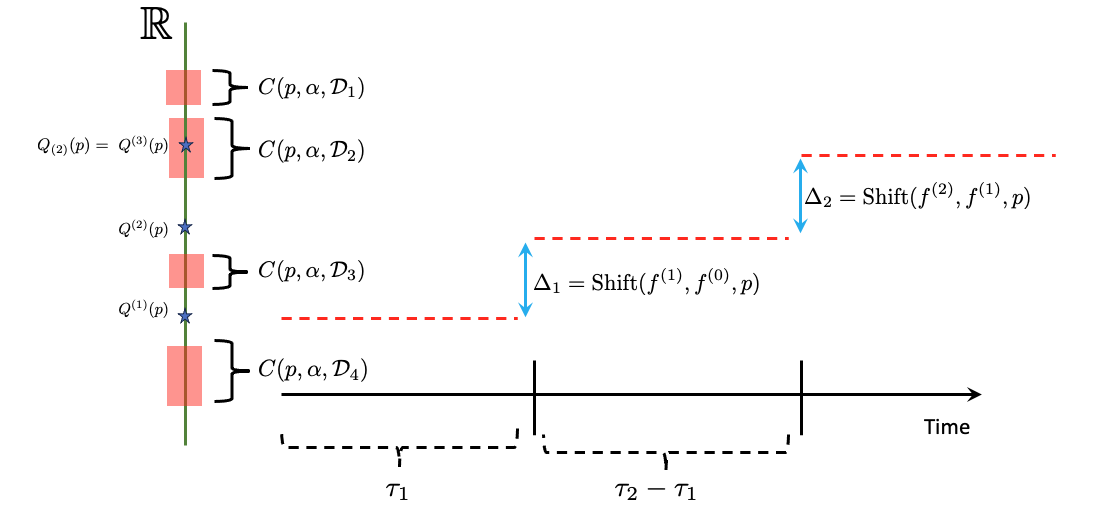
\includegraphics[width=0.9\linewidth]{anomaly/figs/separated_datasets.png}
%     \caption{An illustration of Assumption \ref{asumption_detectable} and \ref{defn:offline_datasets} on a stream with $2$ change-points ($H_T=2)$ and $K=4$ offline datasets. Assumption \ref{asumption_detectable} implies that the change-points on the stream are sufficiently far apart. Assumption \ref{defn:offline_datasets} implies that the $4$ CS do not intersect. Moreover, either the true quantile on the stream are outside the offline CS, i.e., $Q^{(1)}(p)$ and $Q^{(2)}(p)$ are not contained in any offline dataset's CS. Or, it is the case that the online quantile matches one of the offline dataset, i.e., $Q_{(2)}(p) = Q^{(3)}(p)$ in this example.}
%     \label{fig:separated_datasets_example}
% \end{figure}

}

\section{Proof for Theorem \ref{thm:core_theorem}, general case}
{\color{black}



To state performance guarantee of Algorithm \ref{alg:five}, we need a definition of a good event, which occurs with high probability.
\begin{definition}[Good event 4] 
Given a piece-wise stationary sequence $(S_t)_{t=1}^T := \Bigl(T,H_T, (\tau_c)_{c=0}^{H_T}, (f^{(c)})_{c=0}^{H_T}\Bigr)$, with the quantile functions of the $H_T+1$ different segments given by $(Q^{(c)}(\cdot))_{c=1}^{H_T}$ and $K$ offline datasets that are $(p,\alpha)$ separated according to Definition \ref{defn:offline_datasets}, let
% \begin{align}
% \begin{split}
%     \mathcal{E}_4 &:= \bigcap_{k=0}^{H_T} \bigcap_{s = \tau_{k}}^{\tau_{k+2}} \bigcap_{\tau'_k = s}^{\tau_{k+2}} \{ \Tilde{\theta}_{\tau_k:s} \in C_{\tau_k:s} \; \cap  \Tilde{\theta}_{s:\tau'_k} \in C_{s:\tau'_k}\}.\\
%     \end{split}

% \end{align}

\begin{align}
\begin{split}
    \gE_4 = \gG_2 \bigcap \underbrace{\bigcap_{p \in [0,1]}\bigcap_{j=1}^{K} \{ Q_{(k)}(p-u_{N_j}(\alpha)) \leq \widehat{Q}(p, \{ X_l^{(j)} \}_{l=1}^{N_j} ) \leq  Q_{(k)}(p+u_{N_j}(\alpha)) ) \}}_{\text{Offline dataset's CS contain true quantile}}   \\ \underbrace{\bigcap_{k=0}^{H_T}\bigcap_{t_1 = \tau_{k}}^{\tau_{k+1}} \bigcap_{t_2 = t_1 +1}^{\tau_{k+1}}   \bigg\{ \widehat{Q}(p-u_{t_2 - t_1}(\alpha), S_{t_1:t_2})  \leq Q^{(k)}(p) \leq \widehat{Q}(p-u_{t_2 - t_1}(\alpha), S_{t_1:t_2}) \bigg\}}_{\text{Online stream's CS contain true quantile}},
        \end{split}
                \label{eqn:good_event_4_defn}
\end{align}
where the $p$th quantile of the offline datasets $Q_{(l)}(p)$ are defined in Definition \ref{def:offline_quantile} and $\gG_2$ is defined in Equation (\ref{eqn:good_event_G}). 
\end{definition}

%
Event $\gE_4$ is the union of $\gE_2$ in Equation (\ref{eqn:good_event_2_defn}) for the online stream along with the event $\gE_3$ in Equation (\ref{eqn:good_event_3}) for the offline datasets. %The main result of this paper is stated below.

\begin{proposition}
    \begin{align*}
        \mathbb{P}[\gE_4] \geq 1- \alpha (K+2T)
    \end{align*}
    \label{prop:}
\end{proposition}
The proof follows similar to that of Proposition \ref{prop:good_event_2_prob}. 


%In this section, we specify the additional assumption on detectability, which combines the offline and online changes. 
As before, denote by $H_T$ as the number of change points, and the time-instants of change occuring at $1:= \tau_0 < \tau_1 < \tau_2 \cdots < \tau_{H_T} < \tau_{H_T+1}:= T+1$. We denote by the $k$th \emph{online stream} as the stationary samples $\{S_u : \tau_{k-1} \leq u < \tau_{k} \}$. 

For an offline dataset $j \in \{1,\cdots, K\}$ and the online stream $k$, $\Delta^{(j;k)} \geq 0$ denotes the shift between the $j$th offline dataset and the $k$th online stream. As before, similar to Theorem \ref{thm:online_shift}, for all $k \in [H_T]$, denote by $\Delta_{k} = \text{Shift} (f_{k},f_{k+1})$ to be the shift between the $k$th and $k-1$th online segment, and for $k \in [H_T]$ and $j \in [K]$, let $\Delta^{(j,k)} = \text{Shift} (f^{(k)},f_{(j)},p)$ be the shift between the $j$th offline dataset and the $k$th online segment. 
%The main detectability assumption in this section is the following which both Assumptions \ref{asumption_detectable} and \ref{as:offline_detectable}.

% \begin{assumption}[Offline assumption for every stream]
% We will assume that the number of offline dataset samples $N_1, \cdots, N_K$ and the number of online samples $(\tau_k - \tau_{k-1})_{k=1}^{H_T}$ satisfy  
% \begin{enumerate}
%     \item $\tau_{k} - \tau_{k-1} > D(\Delta_{k-1},\alpha) + D(\Delta_k, \alpha) + \max_{1 \leq j \leq K} D(\Delta^{(j;k)}, \alpha) \mathbf{1}(\Delta^{(j;k)} > 0)$
%     \item $N_j \geq \max_{1 \leq k \leq H_T} D(\Delta^{(j;k)}, \alpha) \mathbf{1}(\Delta^{(j;k)}>0)$
% \end{enumerate}
%     \label{as:offline_online_detect}
% \end{assumption}
% In words, the first assumption indicates that each stationary segment is large enough such that the change can be detected by using only the forward and backward confidence, and once a change is detected, the new segment can be matched with an offline dataset if the segment matches one of the offline datasets. The second assumption implies that if a given online segment's $p$th quantile is different from that of a offline dataset, then this change can be detected with high probability. 
% The detectability of this change is reliant on having sufficient number of samples in the offline dataset and thus the assumption is a lower bound on $N_j$. 
}

\begin{theorem*}[\ref{thm:core_theorem}] Let  $(S_t)_{t = 1}^T \sim \Bigl(T,H_T, (\tau_c)_{c=0}^{H_T}, (f_c)_{c=0}^{H_T}\Bigr)$  be a piece-wise stationary stream  satisfying Assumption \ref{asumption_detectable} and offline datasets  $\gD_1, \ldots, \gD_L$ satisfying  Assumption \ref{defn:offline_datasets}. Then, with probability at-least $1-(K+2T)\alpha$, for all times $T \in \mathbb{N}$, Algorithm \ref{alg:five} satisfies %{\em(i)} 
\begin{itemize}
    \item  $\text{FP} + \text{FN}  \leq \sum_{k=1}^{H_T} \left(D(\Delta_{k},\alpha) +  (1-\mathbf{1}_{\text{Match}_k})\max_{ j \in [K]} \left(\lceil \widehat{\tau}_j^{(k)}\rceil \mathbf{1}_{\text{Shift}(f^{(k)},f_{(j)},p) > 0}\right) \right)$ 
    \item Number of abstains less than 
    \begin{align*}
        \sum_{k=1}^{H_T} \Bigl[ &(1-\mathbf{1}_{\text{Match}_k}) 7 \sqrt{(\tau_k-\tau_{k-1}) \ln \left( \frac{1612}{\alpha^2} \ln(e(\tau_k-\tau_{k-1})) \right)}  \\ &+ \mathbf{1}_{\text{Match}_k}\left( 7 \sqrt{(N+T) \ln \left( \frac{1612\ln(e(N+T))}{\alpha^2} \right)}- 4 \sqrt{N \ln \left( \frac{1612\ln(eN)}{\alpha^2} \right)} \right) \\ &+  D(\Delta_{k},\alpha) +  \max_{ j \in [K]} \left(\lceil \widehat{\tau}_j^{(k)}\rceil \mathbf{1}_{\text{Shift}(f^{(k)},f_{(j)},p) > 0}\right)\Bigr],
    \end{align*}
\end{itemize}
where $\mathbf{1}_{\text{Match}_k} = \mathbf{1}_{Q^{(k)}(p) \in \{Q_{(1)}(p), \cdots, Q_{(K)}(p)\}}$, $Q^{(k)}(p)$ is the $p$th quantile of the $k$th segment of the online stream (Defn. \ref{def:piecewise}) and $Q_{(1)}(p), \cdots, Q_{(K)}(p)$ are the $p$th quantiles of the $K$ different offline datasets (Defn. \ref{definition:offline_dataset}).
\end{theorem*}




The proof structure follows a similar path as that of Theorem \ref{thm:online_shift}. Since Assumption \ref{asumption_detectable} holds, we know that Lemma \ref{lem:bdd_delay_change_induction} holds. Thus, we have that {\em(i)} there are no false positive change detections, and {\em(ii)} all changes are detected with a short detection delay. From the description of Algorithm \ref{alg:five}, we know that whenever a change is detected, a new instantiation of Algorithm \ref{alg:four} is started. Thus, the final result is obtained by summing the guarantees in Theorem \ref{thm:setting_3} over the $k$ online segments in addition to the delay taken to detect changes. 
The delay to detect changes are bounded by using Proposition \ref{prop:delay_bound} and Assumption \ref{asumption_detectable}, similar to that done in Theorem \ref{thm:online_shift}. 


% We will prove through induction, that under the good event $\mathcal{E}_4$ and Assumption \ref{as:offline_online_detect},  and {\em(iii)} if an online segment matches an offline dataset, then the match is identified quickly. If on the other hand a segment does not match any offline dataset, then the number of additional mistakes incurred is small. Concretely, the following is the key structural lemma of Algorithm \ref{alg:five}. 

% In order to state the lemma, we recall the notations that we set in the proof of Lemma \ref{lem:bdd_delay_change_induction}. As before, denote by $\tau_1 < \tau_2 \cdots < \tau_k < \tau_{k+1}$ be the set of times at which a true-change occurs. For each $k \in \{1, \cdots, H_T\}$, denote by $\tau_k^{'}$ as the time at which Algorithm \ref{alg:five} detects a change for the $k$th time.

% \begin{lemma}[No false change detections and bounded delay for identifying change and matching offline datasets]
%         Under the event $\mathcal{E}_4$, if Assumption \ref{as:offline_online_detect} holds, then for all $k \in \{1, \cdots, H_T\}$, 
%     \begin{itemize}
%         \item  $\tau_k^{'} \geq \tau_k$, and
%         \item $\tau_k^{'} - \tau_k \leq D(\Delta_k, \alpha)$.
%     \end{itemize}
%     \label{lem:bdd_delay_change_induction_general}
% \end{lemma}

% Before we prove the lemma, we show how this concludes the proof of Theorem \ref{thm:core_theorem}.

\begin{proof}[Proof of Theorem \ref{thm:core_theorem}]
    Theorem 6 is the joint result of theorems \ref{thm:online_shift} and \ref{thm:setting_3}. As in Theorem \ref{thm:online_shift}, Lemma \ref{lem:bdd_delay_change_induction} implies that at time $\tau'_k < \tau_{k+1}$, a new instantiation of Algorithm \ref{alg:four} is started. Theorem \ref{thm:setting_3} states that in the time interval $[\tau'_k, \tau_{k+1}]$, the $k$th online segment incurs a total number of mistakes bounded by the guarantee in Theorem \ref{thm:setting_3} for a time horizon $\tau_{k+1} - \tau'_{k}$. Concretely, in the time-interval $[\tau'_k, \tau_{k+1}]$, the sum of FP and FN is bounded above by $0$ in the event  $\mathbf{1}_{\text{Match}_k}$ holds, and by $\max_{ j \in [K]} \left(\lceil \widehat{\tau}_j^{(k)}\rceil \mathbf{1}_{\text{Shift}(f^{(k)},f_{(j)},p) > 0}\right) $ in the case when $\mathbf{1}_{\text{Match}_k}$ does not hold. %In other words, the sum of FP and FN in the time interval $\tau_{k+1} - \tau_{k}^{'}$ is at-most $\max_{1\leq j \leq K} D(\Delta^{(j;k)}, \alpha)\mathbf{1}(\Delta^{(j;k)} > 0)$. 
    Similarly, the number of abstains in the time-interval $\tau_{k+1} - \tau_{k}^{'}$ is given by the guarantee of Theorem \ref{thm:setting_3}. Now, summing over the $H_T$ different online segments yields the result. 
    
    For any segment $k \in [1, \ldots, H_T]$,  we have 
    \begin{itemize}
        \item $\text{FP}_k + \text{FN}_k  \leq D(\Delta_{k},\alpha) +   1-\mathbf{1}_{\text{Match}_k})\max_{ j \in [K]} \left(\lceil \widehat{\tau}_j^{(k)}\rceil \mathbf{1}_{\text{Shift}(f^{(k)},f_{(j)},p) > 0}\right)$ where the first term is from detection delay in detecting the change (Proposition \ref{prop:delay_bound}) and the second term from Theorem \ref{thm:setting_3}.
        \item If $Q^{(k)}(p)$ matches one of the dataset $\{Q_{(1)}(p), \cdots, Q_{(K)}(p)\}$, then under event $\gG_2$, number of abstains is at-most
        \begin{align*}
           D(\Delta_k, \alpha)+ \max_{ j \in [K]} \left(\lceil \widehat{\tau}_j^{(k)}\rceil \mathbf{1}_{\text{Shift}(f^{(k)},f_{(j)},p) > 0}\right) + 7 \sqrt{(N+\tau_k - \tau_{k-1}) \ln \left( \frac{1612\ln(e(N+\tau_k - \tau_{k-1}))}{\alpha^2} \right)} \\ - 7 \sqrt{N \ln \left( \frac{1612\ln(eN)}{\alpha^2} \right)},
        \end{align*}
        by Theorem \ref{thm:core_theorem}, case $\Delta = 0$.
        \item  If $Q^{(k)}(p)$ matches none of the datasets:
        \[ \text{Abstains} \leq   D(\Delta_k, \alpha)+ \max_{ j \in [K]} \left(\lceil \widehat{\tau}_j^{(k)}\rceil \mathbf{1}_{\text{Shift}(f^{(k)},f_{(j)},p) > 0}\right) + 7 \sqrt{(\tau_k - \tau_{k-1}) \ln \left( \frac{1612\ln(e(\tau_k - \tau_{k-1})))}{\alpha^2} \right)} 
        \]
        by theorem \ref{thm:core_theorem}, case $\Delta > 0$.
    \end{itemize}
The term of $D(\Delta_k, \alpha)$ always shows in all three equations above as that is the amount of time taken for the $k$th change-point to be detected and thus all decisions made during the times of change can potentially lead to mistakes and abstains. Combining the piece-wise results together, we have 
    \begin{align*}
    \text{FP} + \text{FN} \;  \leq \; & \sum_{k=1}^{H_T}D(\Delta_{k},\alpha) + (1-\mathbf{1}_{\text{Match}_k})  \max_{ j \in [K]} \left(\lceil \widehat{\tau}_j^{(k)}\rceil \mathbf{1}_{\text{Shift}(f^{(k)},f_{(j)},p) > 0}\right) 
        \end{align*}
        Similarly, summing over the $H_T$ online segments gives the bound on the number of abstains. 
         % \text{Abstains} \;  \leq \;  &  \sum_{k=1}^{H_t} \Bigl[ (1-\mathbf{1}_{\text{Match}_k}) \mathcal{O}(\sqrt{\tau_k - \tau_{k-1}}) \\ &+ \mathbf{1}_{\text{Match}_k}\left(\gO(\sqrt{N+(\tau_k-\tau_{k-1})} - \sqrt{N}) \right) \\ &+  D(\Delta_{k},\alpha) \Bigr],

\end{proof}

% --------------------------------------------------

% \subsection{Necessity of Assumption \ref{asumption_detectable}  }

% The core of our result requires that the changes are not too often, i.e., there is sufficient gap between changes, quantified precisely in Assumption \ref{asumption_detectable}. We remark that these assumptions are standard in the study of online decision making under non-stationarity \cite{liu2018change, JMLR:v23:20-1384}. This assumption ensures that all changes are detected. However, it is an interesting question to have a non-trivial analysis of dynamic decision making algorithms without assuming that each stationary environment is sufficiently long (Conclusion section of \cite{JMLR:v23:20-1384}). 

\section{Additional Related Works}
\label{app:related}

\paragraph{Online anomaly detection works} There exist works that focuses on other aspects of online anomaly detection. \cite{zhu2023meter} models online concept drift via an ensemble of models.   \cite{nardi2022anomaly} tackles modeling for online AD in a Federated setting. \cite{bhatia2022memstream} studies the low-memory constraint of online AD, and \cite{goyal2020drocc} focuses on efficiently modeling multi-dimensional data. A survey of methodologies of data modelling for AD can be found in the surveys of \cite{chandola2009anomaly, ruff2021unifying, pang2021deep}. Our work differs from these works in setting: we focus on dynamic thresholding of anomaly scores without having access or ability to retrain the underlying AD algorithm.

\paragraph{Threshold learning} Using score thresholds to make binary decision of seeking labels from human experts are studied in active learning \cite{balcan2007margin, zhang2016online,vishwakarma2023promises}. However, active learning does not have a concept of mistakes and is thus have different desiderata compared to our study. 

\section{Additional experiments and experiment details}
\label{app:exp1}

\subsection{Synthetic experiments}
We conduct our synthetic experiments for 1000 trails on streams each of length 1000. The normal distribution online streams are synthesized with parameters sampled uniformly form $[0, 10]$ for mean and $[0.2, 2]$ for variance. The Pareto distributions' parameters are sample uniformly from $[1,3]$ for $b$, $[0,10]$ for mean, and $[0.2,2]$ for scale. To synthesize distribution shifts, we sample a duration for each stationary piece from a Poisson distribution with $\lambda = 300$. To simulate datasets, we prepare $L=5$ offline datasets each of size $N=5000$; the online stream can be generated from either one of the dataset distributions or a random one with uniform probability. The range of these parameters are chosen to simulate real world anomaly score data. The code to generate the synthetic dataset as well as implementations of our algorithms will be open sourced.


\begin{table}[h!]
    \centering

    % \begin{tabular}{c c |c  c |c c}
    % \toprule
    %   & & \multicolumn{2}{|c|}{Normal} & \multicolumn{2}{|c}{Pareto} \\
    %   shift  & data   &  Abs. (\%) & Mis. (\%) &  Abs. (\%) & Mis. (\%)\\
    %   \midrule 
    %  x & x &  18.1 \plusminus{1.1} &  0 \plusminus{0} & 17.8 \plusminus{7.4} & .03 \plusminus{.01}\\
    %  \checkmark & x &   41.7 \plusminus{12.1} &  .05 \plusminus{0} &  51.9 \plusminus{35.0} & .51 \plusminus{.18}\\
    %  x & \checkmark  &  14.3 \plusminus{2.6} &  0 \plusminus{.01}& 16.8 \plusminus{4.7} & .06 \plusminus{.04} \\
    %  \checkmark  & \checkmark  & 32.9 \plusminus{7.1} &  .05 \plusminus{.03} & 24.3 \plusminus{5.2} &  .33 \plusminus{ .41 }\\
    % \bottomrule
    % \end{tabular}
    \begin{tabular}{c c |c c}
\toprule
  & & \multicolumn{2}{|c}{Pareto} \\
  shift & data & Abs. (\%) & Mis. (\%) \\
\midrule
 x & x & 17.8 \plusminus{7.4} & .03 \plusminus{.01} \\
 \checkmark & x & 51.9 \plusminus{35.0} & .51 \plusminus{.18} \\
 x & \checkmark & 16.8 \plusminus{4.7} & .06 \plusminus{.04} \\
 \checkmark & \checkmark & 24.3 \plusminus{5.2} & .33 \plusminus{.41} \\
\bottomrule
\end{tabular}

    \caption{Results of our algorithms on synthetic stream dataset generated from Pareto distribution.}
    \label{tab:synthetic_appendix}
\end{table}

\subsection{Case study of real AD application}
In this section we provide details on our real data experiments. We run Algorithms \ref{alg:two} and \ref{alg:five} on two large scale datasets {\ttfamily DS1} and {\ttfamily DS2} obtained from monitoring two large cloud computing services. Each dataset is a stream of anomaly scores obtained by applying a single anomaly detection algorithm. On these datasets, we run our two general algorithms, Algorithm \ref{alg:two} and \ref{alg:five} with $p = 1 - 10^{-6}$ and $\alpha = 10^{-6}$. Algorithm \ref{alg:five} can use offline datasets. In order to create them, we sampled 50 streams randomly that had length at-least $20,000$ in each of the two datasets. From this collection of $100$ streams, we sub-selected $37$ and $23$ streams from datasets {\ttfamily DS1} and {\ttfamily DS2} respectively such that no two datasets in this collection of $60$ streams overlapped. This is so that Assumption 6.1 is satisfied by the offline dataset. 

The description of the rest of the dataset on which we run the online algorithms is in Table \ref{tab:real_data_stats}. In addition, we also run {\ttfamily DSpot} \cite{siffer2017anomaly} with $p = 1 - 10^{-6}$ and set {\ttfamily num-init} to $500$ and {\ttfamily depth} to $100$ on the online algorithm dataset. All other parameters of {\ttfamily DSpot} was set to the suggested values in \cite{siffer2017anomaly}. In addition to these, we also compare against two static baselines of using the first $500$ and $100$ samples respectively and set the threshold as the max of the observed samples. This threshold is not changed since. 

The results of this experiment are reported in Table \ref{tab:real_data}. From this table, we can see that incorporating offline data reduces the number of abstains for both datasets without changing the volume of anomalies raised. This shows that when there are offline datasets available to the algorithm, the online performance is improved. 


\begin{table}[h!]
    \centering
    \begin{tabular}{c|c|c|c}
    \toprule
     & Num. of Streams & Average stream length &  Total num samples   \\ \midrule 
{DS1}  & $8377$ & $10925.4$ & $91521785$\\ \midrule
{DS2}  & $9657$ &  $10855.6$ & $104832532$\\
         \bottomrule
    \end{tabular}
    \caption{Summary of data properties for real world AD case study.}
    \label{tab:real_data_stats}
\end{table}


\begin{table}[h!]
    \centering

    \begin{tabular}{c|c|c|c| c| c|c}
    \toprule
                &  & Algo 3 & Algo 5 &  DSpot & $\tau^{(1)}$  & $\tau^{(2)}$  \\
        \midrule
         \multirow{2}{*}{DS1}  & Abstains $\downarrow$ & $13.6\%$ & $11.2\%$ & $1.2\%$ & $1.16\%$ & $0.05\%$\\
          & Anomaly $\downarrow$ & $\mathbf{.008\%}$ & {$\mathbf{.008\%}$} & $2.9\%$ & $0.02\%$ & $0.95\%$\\
          \midrule
         \multirow{2}{*}{DS2}  & Abstains $\downarrow$ & $13.3\%$ & $9.9\%$ & $1.3\%$& $1.25\%$ & $1.08\%$   \\
          & Anomaly $\downarrow$ & $.006\%$ & $\mathbf{.005\%}$ & $3.9\%$ & $0.07\%$ & $0.06\%$ \\
         \bottomrule
    \end{tabular}
    
    \caption{Case study performance. All baseline algorithms report anomaly rates much higher than the targeted $10^{-6}$, overwhelming the alarm system. By incorporating offline datasets, we are able to further decrease abstains and achieve a lower rate of reported anomaly. 
    }
    \label{tab:real_data}
\end{table}

\subsection{Additional experiment on open-source datasets}

We include additional experiments as follows. With the same underlying AD scoring algorithm (isolation forest for ForestCover, and a 3-layer MLP for Mammography), our confidence sequence algorithm (Algorithm \ref{alg:marginal_decision} in paper) can achieve a higher F1 score and fewer mistakes, with similar or less number of abstains, compared to a static threshold. This further demonstrates that our thresholding algorithm improves performance across datasets and base anomaly scoring algorithms.


\begin{table}[h!]
    \centering
    \begin{tabular}{ccc|cc}
        \toprule
       &\multicolumn{2}{c}{ForestCover (first 1500 as holdout)} & \multicolumn{2}{c}{Mammography (first 300 as holdout)} \\
        \midrule
        & Ours & Static Threshold & Ours & Static Threshold \\
        \midrule
        Abstain \% & 1.5\% & 1.5\% & 2.1\% & 5\% \\
        FP + FN & 645 & 1603 & 56 & 83 \\
        F1 & 0.39 & 0.33 & 0.51 & 0.43 \\
        \bottomrule
    \end{tabular}
    \caption{Performance comparison of algorithms on ForestCover and Mammography datasets}
    \label{tab:performance}
\end{table}



\section{Proof of Lower Bound}
\label{sec:lower_bound_proof}
The proof is based on the classical hypothesis testing lower bounds due to Neyman and Pearson. Throughout this section, we will fix a $T \in \mathbb{N}$ sufficiently large and let $\mathbb{P}_0 := N(0,1)$  be the standard normal distribution and $\mathbb{P}_{1} := N(\frac{1}{\sqrt{T}},1)$ as an unit variance normal distribution with mean $1/\sqrt{T}$. 

\begin{theorem}[Neyman-Pearson]
For any $T \in \mathbb{N}$, given $T$ i.i.d.. samples $S_{1:T}$, we want to distinguish between the two hypothesis $H_0: S_{1:T} \sim \mathbb{N}(0,1)$ or $H_1: S_{1:T} \sim \mathcal{N}(1/\sqrt{T},1)$. Then, for any measurable function $\mathcal{A} : \mathbb{R}^T \to \{0,1\}$, 
\begin{align*}
   \max( \mathbb{P}_0[\mathcal{A}(S_{1:T}=1], \mathbb{P}_0[\mathcal{A}(S_{1:T}=1]) \geq \frac{1}{4} \exp(-\frac{1}{2}),
\end{align*}
    where $\mathbb{P}_{i}$ for $i \in \{0,1\}$ is the proabability distribution under hypothesis $H_i$.
    \label{thm:neyman_pearson}
\end{theorem}

\begin{lemma}
    For every $p \in (0,1)$, there exists a constant $C_p \in (0,\infty)$ depending only on $p$, such that for $S \sim {N}(0,1)$
    \begin{align*}
        \mathbb{P}[S \in (Q^{(0)}(p), Q^{(1)}(p))] \geq \frac{C_p}{\sqrt{T}},
    \end{align*}
    where $Q^{(0)}(p)$ is the $p$th quantile of a $N(0,1)$ distribution and $Q^{(1)}(p)$ is the quantile of a $N(\frac{1}{\sqrt{T}},1)$ distribution.
    \label{lem:cp_lb}
\end{lemma}

Now, a standard Chernoff bound gives the following result.
\begin{lemma}[Chernoff bound]
Let $T \in \mathbb{N}$ and suppose $S_{1:T}$ are i.i.d., $N(0,1)$ random variables. Let $p \in (0,1)$. Then, 
\begin{align}
    \mathbb{P}\left[ \sum_{t=1}^T \mathbf{1}_{S_t \in (Q^{(0}(p), Q^{(1)}(p))} \leq \frac{C_p\sqrt{T}}{2} \right] \leq \exp \left( \frac{\sqrt{T}}{8} \right),
\end{align}
where $C_p$ is from Lemma \ref{lem:cp_lb}.
    \label{lem:lb_chernoff}
\end{lemma}

\begin{theorem}[Main lower bound]
Denote by two distributions  $\mathbb{P}_0 := N(0,1)$ and $\mathbb{P}_{1} := N(\frac{1}{\sqrt{T}},1)$ as unit variance guassians with means $0$ and $\frac{1}{\sqrt{T}}$ respectively. For $i \in \{0,1\}$, denote by $Q^{(i)}(p)$ as the $p$th quantile of distribution $\mathbb{P}_i$. For a threshold $\theta \in \mathbb{R}$ and sample $x \in \mathbb{R}$, denote by the indicator function $\widehat{Y}_t^{(\theta)}(x) := \mathbf{1}(x \geq \theta)$. Similarly, denote by the indicator function $Y_t^{(i)}(x) = \mathbf{1}(x \geq Q^{(i)})$ for $i \in \{0,1\}$. Let $\mathcal{A}: \mathbb{R}^T \to \{0,1\}$ be any measurable hypothesis testing function. Then, there exists $i \in \{0,1\}$ such that when $S_{1:T}$ are i.i.d. with distribution $\mathbb{P}_i$, then with probability at-least $\frac{1}{8} -  \exp \left( \frac{\sqrt{T}}{8} \right)$,
    \begin{align*}
 \sum_{t=1}^T \mathbf{1} ( \widehat{Y}_t^{(Q^{(\mathcal{A}(S_{1:T}))}(p))}(S_t) \neq Y_t^{(i)}(S_t) ) \geq C_p \sqrt{T},
    \end{align*}
where $C_p$ is from Lemma \ref{lem:cp_lb}.
    \label{thm:main_lower_bound}
\end{theorem}
In words, the above theorem states that even when the true distribution is known to be one of two possibilities and the optimal threshold is chosen using any measurable function, $O(\sqrt{T})$ mistakes is un-avoidable. 

\begin{proof}
Pick $\mathcal{A}: \mathbb{R}^T \to \{0,1\}$ by a measurable function that tests the hypothesis $H_0: S_{1:T}$ are i.i.d. with distribution $\mathbb{P}_0$ and $H_1: S_{1:T}$ are i.i.d. with distribution $\mathbb{P}_1$. From Theorem \ref{thm:neyman_pearson}, we know that for this given test $\mathcal{A}$, there exists $i \in \{0,1\}$ such that
\begin{align}
\mathbb{P}_i[\mathcal{A}(S_{1:T}) \neq i] \geq \frac{1}{8}.
\end{align}
Without loss of generality, lets suppose $i = 0$, i.e., given a hypothesis test $\mathcal{A}$, $\mathbb{P}_0[\mathcal{A}(S_{1:T}) \neq 0] \geq \frac{1}{8}$. We will show in the rest of the proof that for this $\mathcal{A}$, if $S_{1:T}$ are i.i.d. with distribution $\mathbb{P}_0$, $ \sum_{t=1}^T \mathbf{1} ( \widehat{Y}_t^{(Q^{(\mathcal{A}(S_{1:T}))}(p))} \neq Y_t^{(0)} ) \geq C_p \sqrt{T}$ holds with probability at-least $\frac{1}{8} -  \exp \left( \frac{\sqrt{T}}{8} \right)$.

To do so, let $S_{1:T}$ be i.i.d. $\mathbb{P}_0$. From Lemma \ref{lem:lb_chernoff}, we know that 
\begin{align*}
             \mathbb{P}_0\left[ \sum_{t=1}^T \mathbf{1}_{S_t \in (Q^{(0}(p), Q^{(1)}(p))} \leq \frac{C_p\sqrt{T}}{2} \right] \leq \exp \left( \frac{\sqrt{T}}{8} \right). 
\end{align*}
Thus, from an union bound, we know that for the given $\mathcal{A}$,
\begin{align*}
    \mathbb{P}_0 \left[ \underbrace{\mathcal{A}(S_{1:T}) \neq 0,  \sum_{t=1}^T \mathbf{1}_{S_t \in (Q^{(0}(p), Q^{(1)}(p))} \geq \frac{C_p\sqrt{T}}{2}  }_{\text{Event }\mathcal{H}}\right] \geq \frac{1}{8} - \exp \left( \frac{\sqrt{T}}{8} \right). 
\end{align*}

Observe that under event $\mathcal{H}$, for all $x \in \mathbb{R}$, we have the equality

\begin{align*}
     \mathbf{1} ( \widehat{Y}_t^{(\mathcal{A}(S_{1:T}))}(x) \neq Y_t^{(0)}(x) ) = \mathbf{1} (x \in (Q^{(0)}(p), Q^{(1)}(p)).
\end{align*}
Thus, under event $\mathcal{H}$, we have 
\begin{align*}
    \sum_{t=1}^T \mathbf{1} ( \widehat{Y}_t^{(\mathcal{A}(S_{1:T}))}(S_t) \neq Y_t^{(0)}(S_t) ) = \sum_{t=1}^T \mathbf{1}_{S_t \in (Q^{(0}(p), Q^{(1)}(p))} \geq \frac{C_p\sqrt{T}}{2},
\end{align*}
holding with probability at-least $\frac{1}{8} - \exp \left( \frac{\sqrt{T}}{8} \right).$
\end{proof}

%\subsection{Discussion of the lower bound}

The theorem asserts that if an algorithm does not abstain, then even in a stationary stream, $O(\sqrt{T})$ mistakes will occur with high probability. 


%\bibliographystyle{plain}
%\bibliography{ref}



\chapter{Learning for Mechanical Circulatory Support (MCS) devices}


\chapter{Uncertainty Quantification for Large Language Model Assistants}



% \part{Exploring Ambiguity in Creative AI}
% \chapter{Karaoke of Dreams}
% \chapter{Learning to Move, Learning to Play, Learning to Animate}

\part{Conclusion and Future works}
\chapter{Summary and Discussion}
\chapter{Future Works}

\appendix

% Stuff at the end of the dissertation goes in the back matter
\backmatter
\bibliographystyle{plain} % Or whatever style you want like plainnat
\bibliography{references}

\end{document}
